\documentclass[10pt,a4paper]{article}
\usepackage[margin=15mm]{geometry}\usepackage{fontspec,amsmath,amssymb,graphicx,booktabs,longtable,hyperref}
\setmainfont{Latin Modern Roman}\setlength{\parindent}{0pt}\setlength{\parskip}{5pt}\hypersetup{colorlinks=true,linkcolor=blue,pdftitle={APD consolidated model and background-cap comparison}}\setcounter{tocdepth}{1}
\begin{document}
{\LARGE APD background and interference models}\par
{\large Consolidated cap-sweep draft: exact and local angular diagnostics}\par 7 October 2026 · for discussion with Richard

This draft compares ten model families where available, using the same gain-corrected reference construction and intensity objective. Its purpose is to expose the trade-off between forward agreement, background budget and stability of recovered orientations. No model supplies independently validated rod angles.

\textbf{Reading order.} Each model has equations and an explicit list of fitted quantities, a cap summary, then one full page per tested budget. Each case page shows measured-space fits (top), corrected signal space (middle), and signal/background/interference composition (bottom), in 30--31 s and 10--11 s columns. A representative sphere/residual page follows. Tables show actual fitted powers, not merely their allowed caps.

\textbf{Scope.} The primary sweep includes no BG, additive BG, Richard four-C, additive plus bounded interference, uniform pupil, three-mode, five-mode, general stationary, edge-localized pupil and bounded axial-motion families. Earlier mask, unconstrained-overlap and inverse-circle tests are summarized as diagnostics rather than mixed into the cap ranking. Superseded reference-coordinate fits and free per-point brightness are not treated as current results.

\textbf{Uncapped means uncapped.} No finite upper bound is imposed on $B_{tot}$ in the new uncapped fits. Earlier ``broad cap'' figures instead imposed $B_{tot}<0.95\min T_{obs}$ and are not relabelled uncapped. Numerical bounds remain on geometry and brightness; finite local solutions do not prove global identifiability.

\textbf{Adaptive sweep.} Test 5\% and 10\% for every model with a defined additive background power. If neither produces radial exceedance or negative corrected channels in either training or held-out window, test 20\%,30\%,\ldots until the first tested failure. The first failing case is included. Stop also if the cap becomes inactive and reproduces an admissible uncapped solution. No-BG and Richard have no BG-power cap to vary. This is an exploratory path through local solutions, not a proof that every solution below a threshold is valid or every solution above it fails. Held-out data now help decide which budgets to explore; they are repeatability diagnostics, not untouched validation data.

\textbf{Failure definition.} A radial exceedance is $r>r_{sat}+10^{-8}$ with $r_{sat}=0.92778057$. Negative corrected channels are tracked as a separate failure. No physical clipping is performed. Plot triangles mark off-axis data; axes remain $[-1,1]$ in both anisotropy directions. Tiny numerical exceedances and large failures should be distinguished using the composition/metric files.

\tableofcontents
\newpage
\section{Processing, calibration and common objective}
Raw APD channels are reordered from $(90,45,135,0)$ to $(0,90,45,135)$. Gains act before the unchanged inverse transmission matrix. A single pooled training pair-balance adjustment multiplies the historical inverse gains by $(0.992729,1.005313,1.009114,0.992952)$, with product one. Gains are then frozen for every model and interval. Held-out pair imbalance remains about 0.30\% RMS; this is conditional pair-balance calibration, not independent proof of detector gains or absence of path-specific background.

Retain complete-cycle detection and original ordered channel bins: 304 cycles (152/152 alternating train/test) at 30--31 s and 217 (109/108) at 10--11 s. Apply the new calibration to cached four-channel means; average training and held-out groups separately. Rebuild uniform final-reference arc from training data. No current fit changes cycle selection.

Interpolate the four training channels together, including last-to-first, then calculate
\[
X=\frac{I_0-I_{90}}{I_0+I_{90}},\qquad Y=\frac{I_{45}-I_{135}}{I_{45}+I_{135}}.
\]
Integrate ordered XY distance on this interpolant and select 128 equal arc fractions. Carry all four interpolated intensities into the reference. Apply identical original-bin interpolation weights to held-out means, which are not independently re-uniformized. Both loops and repeated passes retain their order. This operation introduces correlated neighboring points, not new independent observations.

For each proposed physical model simulate a full mechanical revolution, form measured-model channels and anisotropy, then sample its own ordered arc at $(\delta+\epsilon u_j)\bmod1$. The measured points and training-derived coordinates $u_j$ remain fixed. One cyclic offset per window, no 16-parameter correspondence warp or independent nearest-point assignment. Current restarts retain historical traversal directions; these local searches are not exhaustive over every initialization.

Let $\varepsilon=I^{obs}-I^{pred}$, and evaluate the fitted correction at the matched cone direction:
\[
\widehat{\mathbf S}=\mathbf I^{obs}-\mathbf B-\mathbf I_{\mathrm{int}}(\mathbf d^{fit})=\mathbf S^{fit}+\boldsymbol\varepsilon.
\]
The fit objective, applied to training means only, is
\[
J=\sum_{ij}\left(\frac{\varepsilon_{ij}}{T_j^{obs}}\right)^2
+100\sum_j\left[\max\left(0,\frac{\widehat r_j-r_{sat}}{1-r_{sat}}\right)\right]^6
+10\sum_{ij}\left[\frac{\min(0,\widehat S_{ij})}{T_j^{obs}}\right]^2.
\]
The radial penalty is exactly zero inside $r_{sat}$ and 100 per point at $r=1$. It uses a pair-denominator guard $10^{-4}T^{obs}$ near zero to avoid numerical singularities; diagnostic ratios use unmodified channels. Negative predicted measured channels are additionally penalized in phenomenological intensity models. Signal-relative RMS is reported only, not minimized. No weights were tuned on the held-out score for each case.

The common-field optical families enforce pair balance for $\mathbf S$, $\mathbf B$ and $\mathbf I_{\mathrm{int}}$ separately by construction. Additive BG also has equal pair sums. Independent-channel Richard/overlap coefficients are explicit phenomenological exceptions and are not silently redefined as common-field models.

Physical field backgrounds are shared across intervals; simple intensity corrections are fitted per interval. Thus parameter sharing differs and model fit quality is not a complexity-adjusted statistical comparison. Field caps use the smaller original calibrated training $T_{max}$, satisfying the cap in both windows; simple models use each window's own $T_{max}$.
\newpage
\section{Signal and field composition}
\subsection*{Notation: scalars, vectors and spatial fields}
Bold symbols denote vectors or matrices; plain components and channel-indexed intensities are scalars.
\begin{center}\begin{tabular}{lp{112mm}}\toprule
Symbol & Type and meaning\\\midrule
$\mathbf d,\mathbf k,\mathbf e_1,\mathbf e_2$ & Real three-vectors: rod direction, cone axis and orthonormal cone basis.\\
$\boldsymbol\xi$ & Two-dimensional pupil position; not a polarization vector.\\
$\mathbf E_b(\boldsymbol\xi),\mathbf U_m(\boldsymbol\xi)$ & Two-component complex polarization fields, defined at every pupil position. The mode patterns are fixed.\\
$b_m$ & Complex scalar coefficient fitted for mode $m$: amplitude and phase.\\
$\mathbf a_i$ & Real two-component analyser vector.\\
$E_{b,i},E_{s,i}$ & Complex scalar spatial fields after projection onto analyser $i$.\\
$I_i,S_i,I_{\mathrm{int},i},B_i,N_i$ & Real scalar channel intensities after spatial integration; only the interference contribution can have either sign.\\
$\mathbf I,\mathbf B$ & Four-component channel lists, not directions in physical space.\\
$\mathbf e_j,\mathbf J_j$ & Two-component anisotropy residual and its $2\times2$ local angular Jacobian.\\\bottomrule
\end{tabular}\end{center}
The distinction before and after an analyser is
\[
\mathbf E_b(\boldsymbol\xi)=\sum_m b_m\mathbf U_m(\boldsymbol\xi),\qquad
E_{b,i}(\boldsymbol\xi)=\mathbf a_i^{\mathsf T}\mathbf E_b(\boldsymbol\xi).
\]
Pupil arguments are suppressed below when unambiguous. Components such as $d_x,d_y$ remain plain scalars. $I_{\mathrm{int},i}$ replaces the former symbol $L_i$ for the complete interference intensity, including brightness. $\mathcal{L}_i$ is a linear optical operator, not that intensity.

\textbf{Noninterfering does not mean unpolarized.} The extra $N_i$ in physical field models is a potentially polarized common optical background with a positive Stokes constraint. Unpolarized light is its equal-channel special case. Independent detector offsets or downstream path backgrounds need not obey this common-field restriction. The standalone additive model uses the looser equal-pair-sum square constraint, as requested.

\textbf{Why these models?} Richard proposed the constant four-$C_i$ effective approximation and discussed unknown phase and spatial variation. The uniform, dipole-mode and general stationary bases are our chosen approximations to those possibilities, not a catalogue of the only possible sources or models prescribed by Richard. The ten-mode basis frees scalar spatial patterns in each polarization; it is not strictly the five-mode basis plus five new modes, since the uniform patterns need not lie in its span.
\newpage

A fixed cone is parameterized by its axis (two angles) and opening $\lambda$:
\[
\mathbf d(\chi)=\cos\lambda\,\mathbf k+\sin\lambda(\cos\chi\,\mathbf e_1+\sin\chi\,\mathbf e_2).
\]
\[
Q_i=A_F+B_F\sin^2\theta+C_F\sin^2\theta\cos2(\phi-\psi_i),
\qquad S_i=a_0^2\sin^2\theta Q_i.
\]
\[
T_S=4a_0^2\sin^2\theta(A_F+B_F\sin^2\theta).
\]
One fitted brightness $a_0$ per interval. The excitation factor $\sin^2\theta$ is not an independent per-point brightness. $A_F=0.890806$, $B_F=0.109194$, $C_F=0.927781$. NA0.38--1.3, water/oil1.33/1.51, Fresnel and corrected BFP mapping are held fixed. Physical field families use common numerical pupil quadrature; the analytic scalar formula differs slightly through quadrature, not through a changed optical model.

For every physical field family,
\[
E_{s,i}=a_0(d_x+\mathrm i d_y)\mathcal{L}_i \mathbf d,\qquad \mathbf{E}_b=\sum_m b_m\mathbf{U}_m,
\]
\[
I_i=\underbrace{\|E_{s,i}\|^2}_{S_i}
+\underbrace{2\operatorname{Re}\langle E_{s,i},E_{b,i}\rangle}_{I_{\mathrm{int},i}}
+\underbrace{\|E_{b,i}\|^2+N_i}_{B_i},
\]
\[
N_i=\frac{N_{tot}}4[1+P\cos2(\psi_i-\gamma)],\quad0\leq P\leq1,
\qquad T=T_S+\sum_iI_{\mathrm{int},i}+B_{tot}.
\]
The detector norm/inner product integrates spatial intensity/overlap; fields are not summed across independent detector pixels before squaring. $B_i$ and $N_i$ are constant, while $S_i,I_{\mathrm{int},i}$ vary with orientation (and height in the axial family). The field parameterization uses total BG power, coherent fraction, $P,\gamma$, and $2m-1$ real angles for a normalized complex $m$-vector: $2m+3$ shared BG parameters. Coherent fractions are conditional fitted allocations, not measured source fractions.

Channel BG values in each model table are percentages of the original measured maximum, in $(0,90,45,135)$ order. Signal and cross-term ranges refer to sums over channels at matched reference positions. Their extrema need not occur at the same point, so range endpoints should not be added together.

\subsection*{Sphere and residual interpretation}
For corrected channels, $\sin^2\widehat\theta=A_Fr/(C_F-B_Fr)$ and $\widehat\phi=\tfrac12\arg(X+\mathrm iY)$. Negative channels or an out-of-range sine square are excluded from the sphere plot, counted and marked; never clipped. Choose among $\phi,\phi+\pi$ and $\theta,\pi-\theta$ jointly along the ordered cycle. Dynamic programming minimizes the sum of squared angular steps divided by their reference-arc spacing, without forcing the last point back onto the first branch. The matched cone only breaks ties between equally smooth branch sequences. At the seam, the initial anisotropy is lifted onto the branch nearest the final direction; its separation from the initial direction is reported as the oriented closure mismatch (the head--tail-equivalent rod mismatch is the smaller of this angle and its supplement). A continuous lift need not close: one winding of anisotropy about the origin changes $\phi$ by $\pi$. For example, the no-BG reconstruction cannot be made both continuous and closed here. This supersedes the earlier pointwise snapping diagnostic. No points are projected onto the cone or moved to close a gap. Invalid points remain excluded; continuity across an invalid interval is not measured. This continuity convention cannot establish the true polar-angle branch, especially near a turning point or equator crossing. Sphere residuals are recomputed using this revised convention.

Sphere plots retain laboratory tilt. In the cone frame, with circle centre $\mathbf c=\cos\lambda\,\mathbf k$, the elevation residual is
\[
\beta=\operatorname{atan2}(\widehat d'_z-\cos\lambda,\sqrt{\widehat d_x'^2+\widehat d_y'^2}).
\]
The second residual is $\sin\lambda\operatorname{wrap}(\widehat\chi-\chi^{fit})$, measuring displacement around the matched circle. These plots are conditional subtraction diagnostics; interference has not been re-solved self-consistently at each corrected direction. Valid-only angular RMS cannot rank models with different excluded subsets.
\newpage\subsection*{Local cone-referenced angular residuals}
This additional diagnostic tests a local approximation alongside exact inversion. At each matched fitted cone direction $\mathbf d_j$, take the corrected held-out anisotropy minus the fitted signal anisotropy:
\[\mathbf e_j=XY(\mathbf I^{heldout}_j-\mathbf B-\mathbf I_{\mathrm{int},j}^{fit})-XY(\mathbf S_j^{fit}).\]
The interference term is still evaluated at the fitted direction. This is a conditional diagnostic, not a self-consistent refit of interference.

Let $\mathbf k$ be the fitted cone axis, $\lambda$ its half-angle, and define unit tangent directions
\[\mathbf t_\perp=(\cos\lambda\,\mathbf d-\mathbf k)/\sin\lambda,\qquad \mathbf t_\parallel=(\mathbf k\times \mathbf d)/\sin\lambda.\]
The first points towards increasing cone angle; the second follows increasing mechanical phase. Using the signal-only anisotropy map $F(\mathbf d)$, calculate its local two-by-two Jacobian and solve
\[\mathbf J_j=\left[\partial_{\mathbf t_\perp}F\quad\partial_{\mathbf t_\parallel}F\right],\qquad
\begin{pmatrix}\delta\lambda\\\delta s\end{pmatrix}=\mathbf J_j^{-1}\mathbf e_j,
\qquad \delta s\simeq\sin\lambda\,\delta\psi.\]
This uses anisotropy residuals, not a new four-channel intensity objective. It does not constrain total brightness or pair balance. Brightness factors cancel in signal anisotropy. The analytic annular Fourkas map is used consistently for the derivative; residuals are measured relative to the actual numerical fitted signal so quadrature differences do not create a spurious zero-residual shift.

To display the displacement on the unit sphere, use its tangent-plane exponential map:
\[\mathbf v=\delta\lambda\,\mathbf t_\perp+\delta s\,\mathbf t_\parallel,\quad a=\|\mathbf v\|,\qquad
 \mathbf d_{local}=\cos a\,\mathbf d+\frac{\sin a}{a}\mathbf v.\]
This stays on the sphere but need not stay on the cone. No clipping, smoothing or residual shrinkage is applied. This is a first-order angular estimate, not an exact inverse. It can form a closed path because the reference geometry and residual are periodic; closure here is not independent evidence that the model is correct.

\textbf{Check the approximation.} Re-evaluate the nonlinear signal map and calculate
\[\eta_j=\frac{\|F(\mathbf d_{local})-F(\mathbf d_j)-\mathbf e_j\|}{\max(\|\mathbf e_j\|,10^{-8})}.\]
A small $\eta$ means the displayed local displacement reproduces the requested anisotropy change. Red points flag any of: angular step above $15^\circ$, $\eta>25\%$, Jacobian condition number above100, rank deficiency, or invalid corrected channels/radius. These are explicit exploratory caution thresholds, not confidence intervals. Exponential mapping of large steps can wrap around the sphere and is not physically trustworthy. The lower panel exposes this instead of hiding it.

\textbf{Comparison.} Grey points show the previous continuous exact inverse, where valid; blue/red points show the local approximation. Red points may be drawn even when exact inversion is invalid: these are extrapolations, not newly valid measurements. The middle panels show local tangent components, not the earlier circle-centre elevation $\beta$.


\newpage
\section{Sweep overview}
\subsection*{Discuss first if time is limited}
\textbf{1. General stationary field, 10\% cap (fit p.~\pageref{case:general:10pct}; local residual p.~\pageref{local:general}).} This is the main stationary-field candidate: corrected held-out points remain valid in both windows, and local angular RMS is2.91/3.48 degrees with 0/128 caution flags in each. Discuss whether the improvement warrants the 33 fitted parameters and what experiment could distinguish this field from other explanations. Compare 5\% and 10\% before the high-budget solutions; a good fit alone does not establish the actual background.

\textbf{2. General field with axial motion, 10\% cap (fit p.~\pageref{case:axial:10pct}; local residual p.~\pageref{local:axial}).} Forward agreement improves further, with local angular RMS 1.66/2.79 degrees and no caution flags. The key question is physical: is the fitted height-dependent phase plausible? Radius is bounded at 300 nm, the waist and 2-micron focus scale are assumed, and the 10--11s radius reaches its bound. This is a sensitivity result, not evidence that the rod follows the fitted height trajectory.

\textbf{3. No BG versus additive BG at 10\% (fits pp.~\pageref{case:none:uncapped},\pageref{case:square:10pct}; local residuals pp.~\pageref{local:none},\pageref{local:square}).} These anchor how much is achieved without interference. NoBG gives about 20 degrees local RMS and 62/63 flagged bins; additive 10\% gives 10.58/12.96degrees and 20/41 flags. The noBG exact inverse also fails closure. Discuss which residual features genuinely require interference, rather than judging only whether the displayed local path looks closed.

\textbf{4. Richard's exact four-$C_i$ approximation (fit p.~\pageref{case:richard_product:uncapped}; local residual p.~\pageref{local:richard_product}).} Include this to answer the original proposal directly. It has no additive BG-power cap; corrected held-out invalid counts are 3/14, and 107/111 local estimates trigger caution. Discuss whether the constant-coefficient approximation is adequate and its brightness/coefficient ambiguity. Do not interpret its unstable local angular RMS as a measured rotation.

\textbf{If there is extra time: five-mode10\% (p.~\pageref{case:five:10pct}).} It provides a lower-dimensional comparison with the general field: 23 versus 33 fitted parameters. Local RMS is 9.96/10.19degrees with 25/30 flags despite no pointwise invalid corrected channels. This illustrates why radius validity alone is insufficient.

These are discussion priorities, not a validated ranking of physical truth. Values are 30--31s /10--11s; all local flags use the explicit approximation checks in Section 2. No refits were performed for the local residual diagnostic.
\newpage
\begin{longtable}{p{52mm}p{35mm}p{70mm}}\toprule
Model & Tested finite caps & Stopping observation\\\midrule\endhead
No background & Not applicable & No BG-power cap applicable\\
Additive background & 5, 10, 20 & First tested failure at 20\%\\
Richard four-C & Not applicable & No BG-power cap applicable\\
Additive plus bounded interference & 5, 10 & First tested failure at 5\%\\
Uniform pupil field & 5, 10, 20 & First tested failure at 20\%\\
Three-mode field & 5, 10, 20, 30, 40, 50 & First tested failure at 50\%\\
Five-mode field & 5, 10, 20, 30, 40, 50 & First tested failure at 50\%\\
General stationary field & 5, 10, 20, 30, 40, 50 & First tested failure at 50\%\\
Hole-edge field & 5, 10, 20, 30 & First tested failure at 30\%\\
General field with axial motion & 5, 10, 20, 30, 40 & First tested failure at 40\%\\
\bottomrule\end{longtable}
These observations apply to the selected local fit at each cap and either-window/train-or-test validity. They do not establish a unique optimal background or a sharp physical threshold. All uncapped solutions are reported as well. Nonconvergence is printed on case pages and in tables. Old results with different correspondence, gain or objectives are not substituted for missing new cases.
\newpage
\section{No background}
\[I_i=S_i,\qquad T=T_S.\]
Fit only the cone (three parameters), brightness $a_0$ and cyclic offset for each window. This is the reference for whether adding a correction actually improves the measured intensities. There is no background parameter to cap.
\textbf{Total fitted continuous parameters across both windows: 10.} The three pre-estimated gain adjustments are additional calibration parameters, held fixed here.
\begin{longtable}{llrrrrrr}\toprule
Budget & Window & BG\% & Meas.RMS & Signal RMS & Bad(train/test) & Max $r$ & Conv.\\\midrule\endhead
uncapped & 30s & 0.0 & 0.0759 & 0.0920 & 0/0 & 0.688 & yes \\
uncapped & 10s & 0.0 & 0.0750 & 0.0895 & 0/0 & 0.679 & yes \\
\bottomrule\end{longtable}
\begin{longtable}{llrrrr}\toprule
Budget & Window & Signal\% range & Cross\% range & Noninterf.BG\% & Fitted folded $\theta$\\\midrule\endhead
uncapped & 30s & 50.1--109.0 & 0.0--0.0 & --- & 30.3--47.0$^\circ$ \\
uncapped & 10s & 54.6--104.7 & 0.0--0.0 & --- & 31.3--45.2$^\circ$ \\
\bottomrule\end{longtable}
\textbf{Per-channel constant background, percent of measured maximum:}
\begin{longtable}{llrrrr}\toprule
Budget & Window & $B_0$ & $B_{90}$ & $B_{45}$ & $B_{135}$\\\midrule\endhead
uncapped & 30s & 0.00 & 0.00 & 0.00 & 0.00\\
uncapped & 10s & 0.00 & 0.00 & 0.00 & 0.00\\
\bottomrule\end{longtable}
\newpage
\subsection{No BG-power cap}\label{case:none:uncapped}
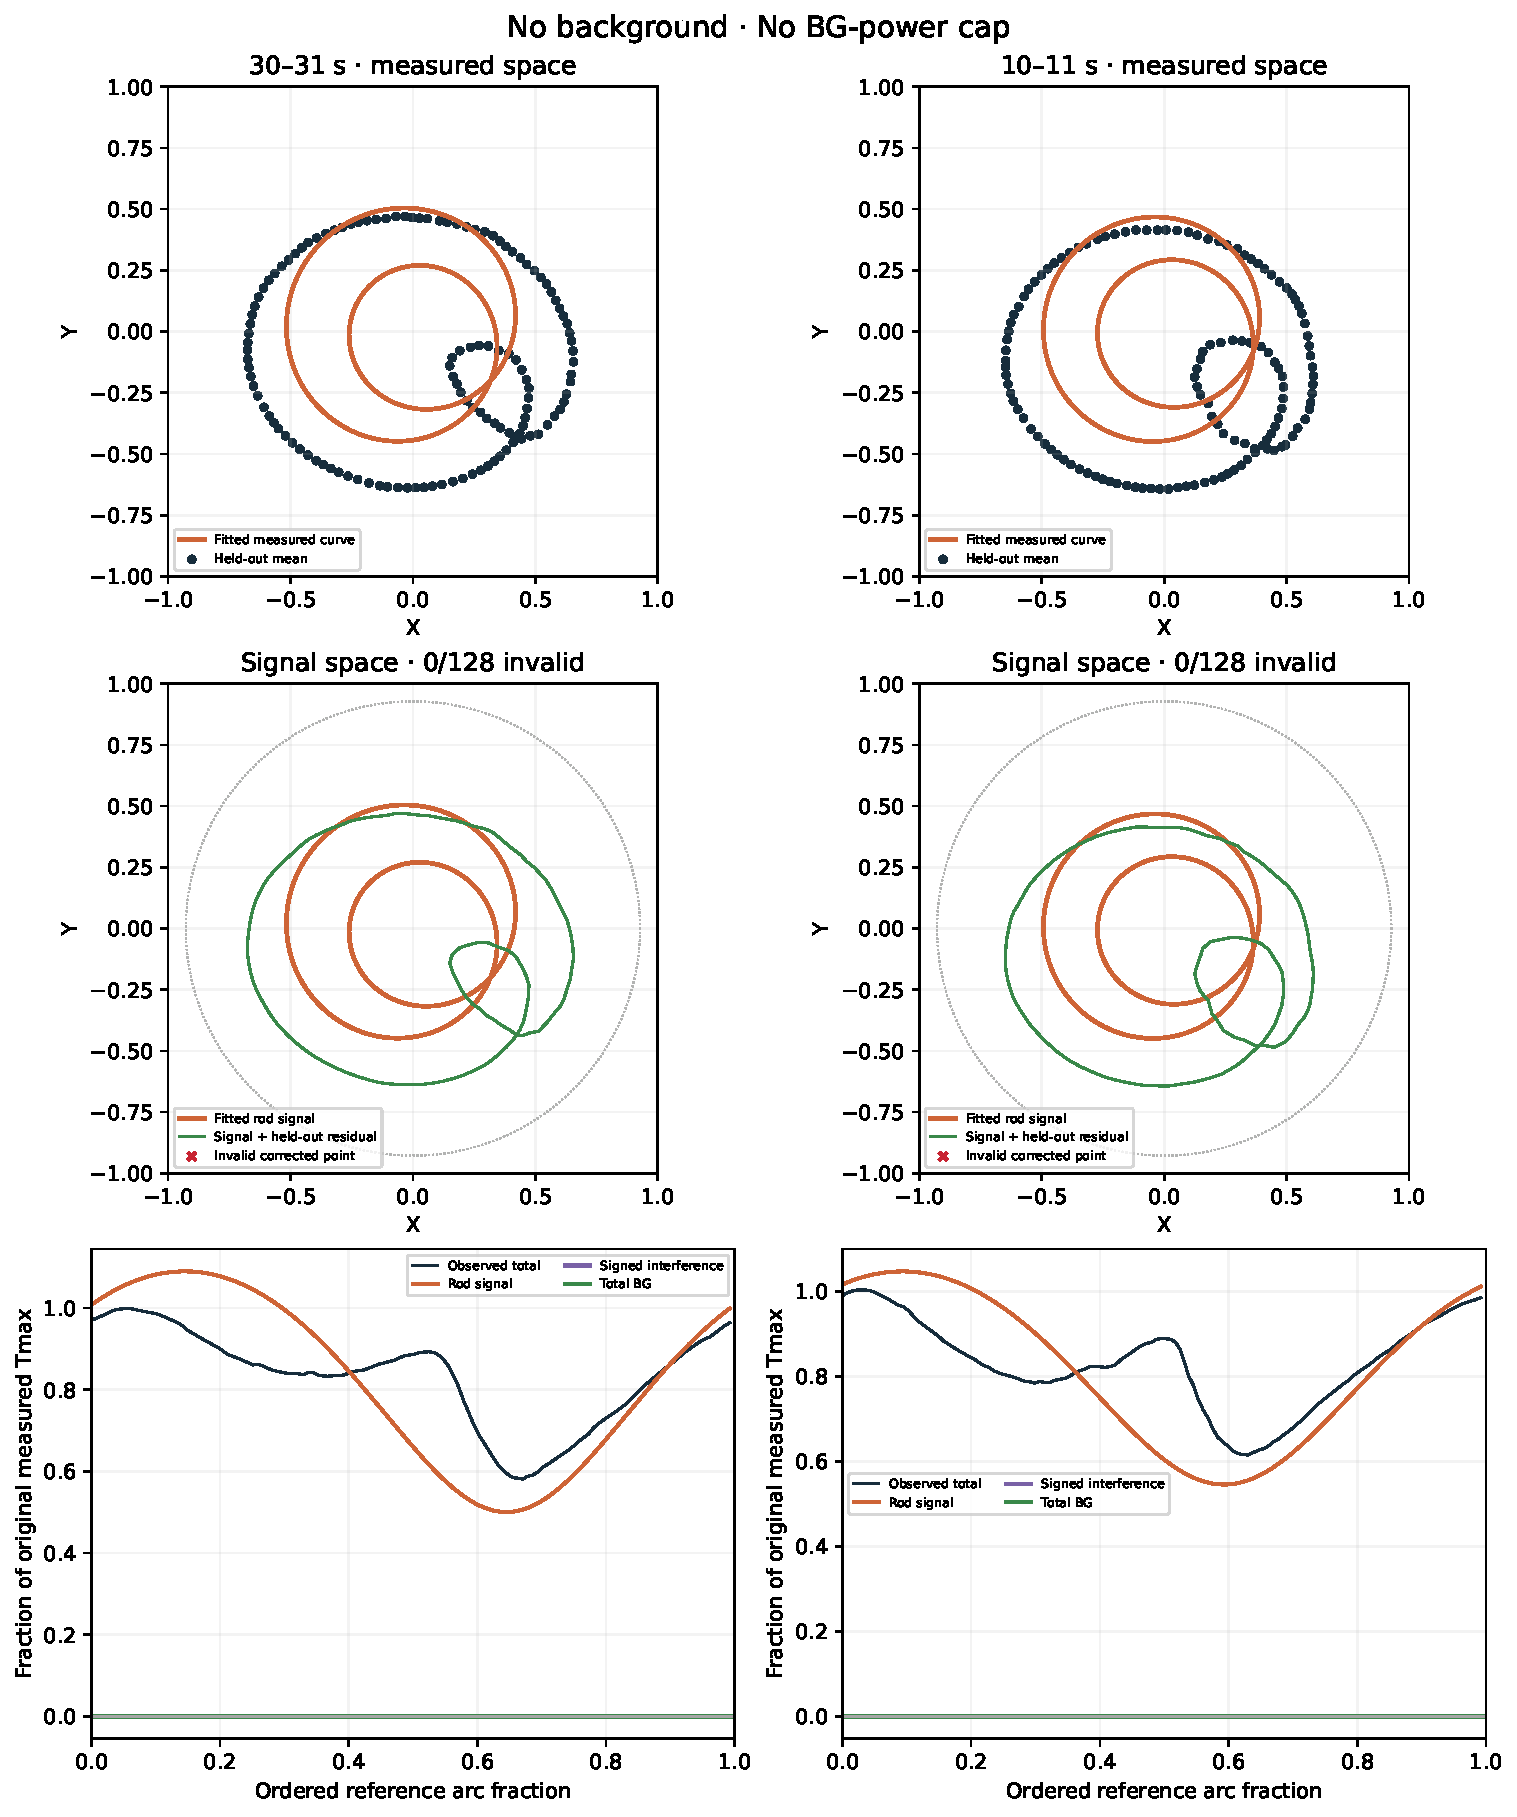
\includegraphics[width=\linewidth,height=.9\textheight,keepaspectratio]{figures/none_uncapped.pdf}
\newpage
\subsection{Representative sphere diagnostic: No BG-power cap}
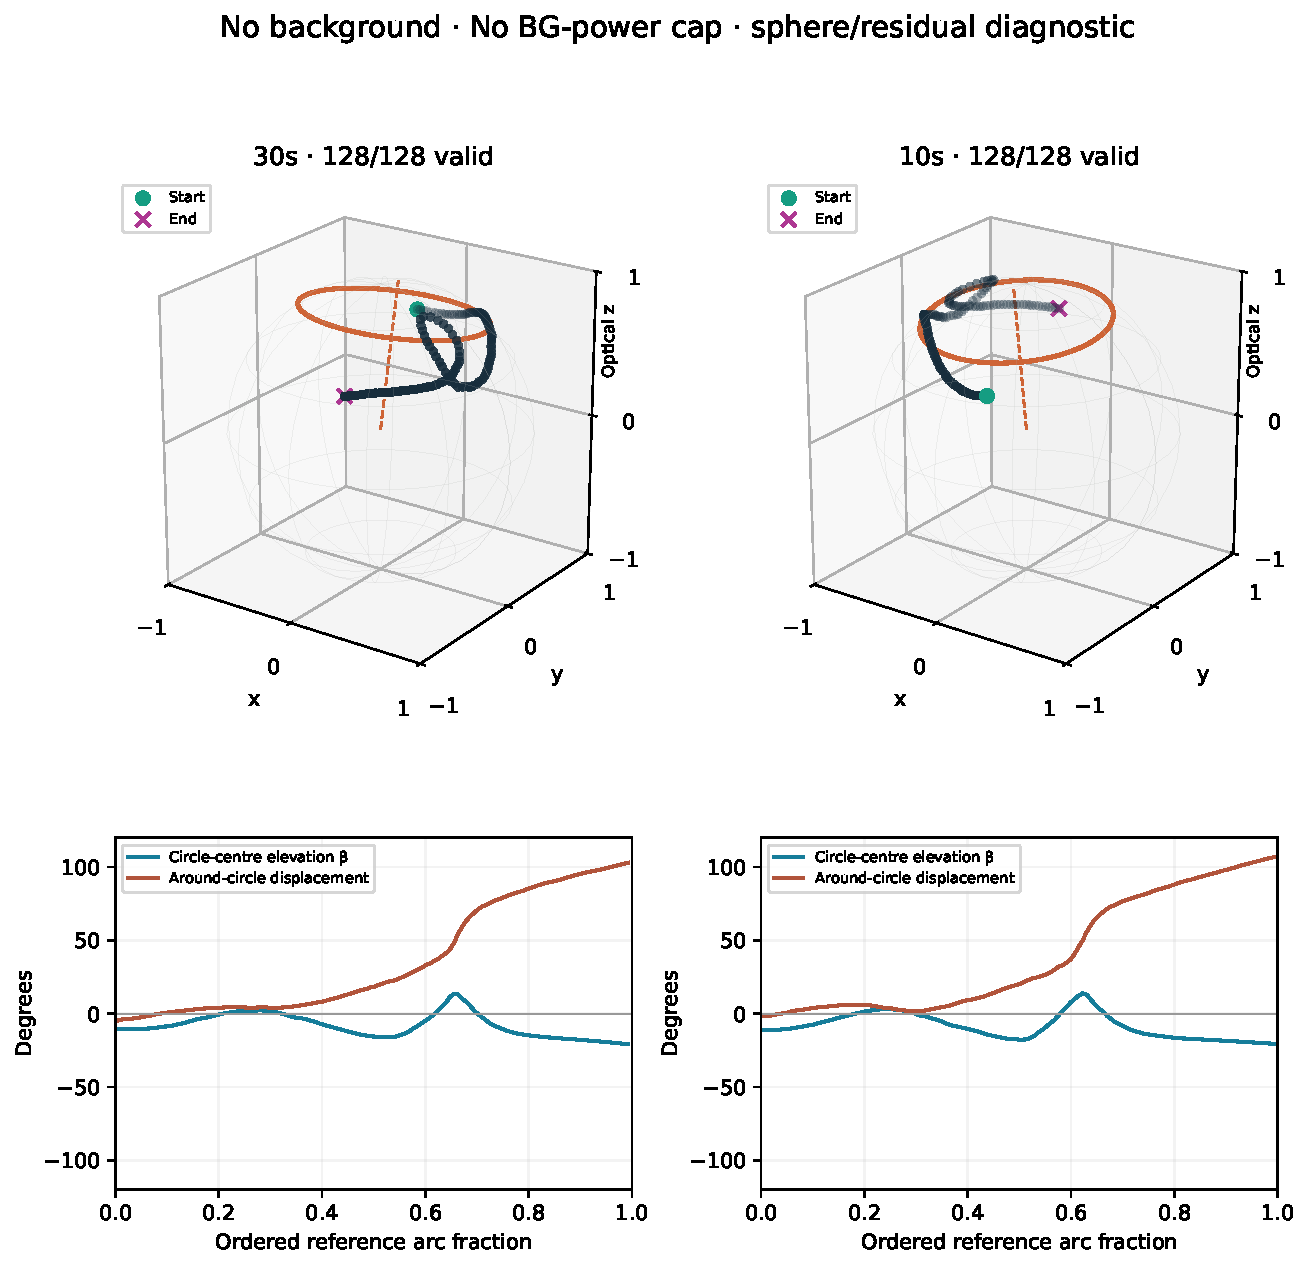
\includegraphics[width=\linewidth,height=.82\textheight,keepaspectratio]{figures/none_sphere.pdf}
30s: 128/128 valid; matched geodesic RMS 52.02$^\circ$; oriented closure mismatch 114.39$^\circ$.\par
10s: 128/128 valid; matched geodesic RMS 54.71$^\circ$; oriented closure mismatch 113.94$^\circ$.\par
\newpage
\subsection{Local cone-referenced angular residual: No BG-power cap}\label{local:none}
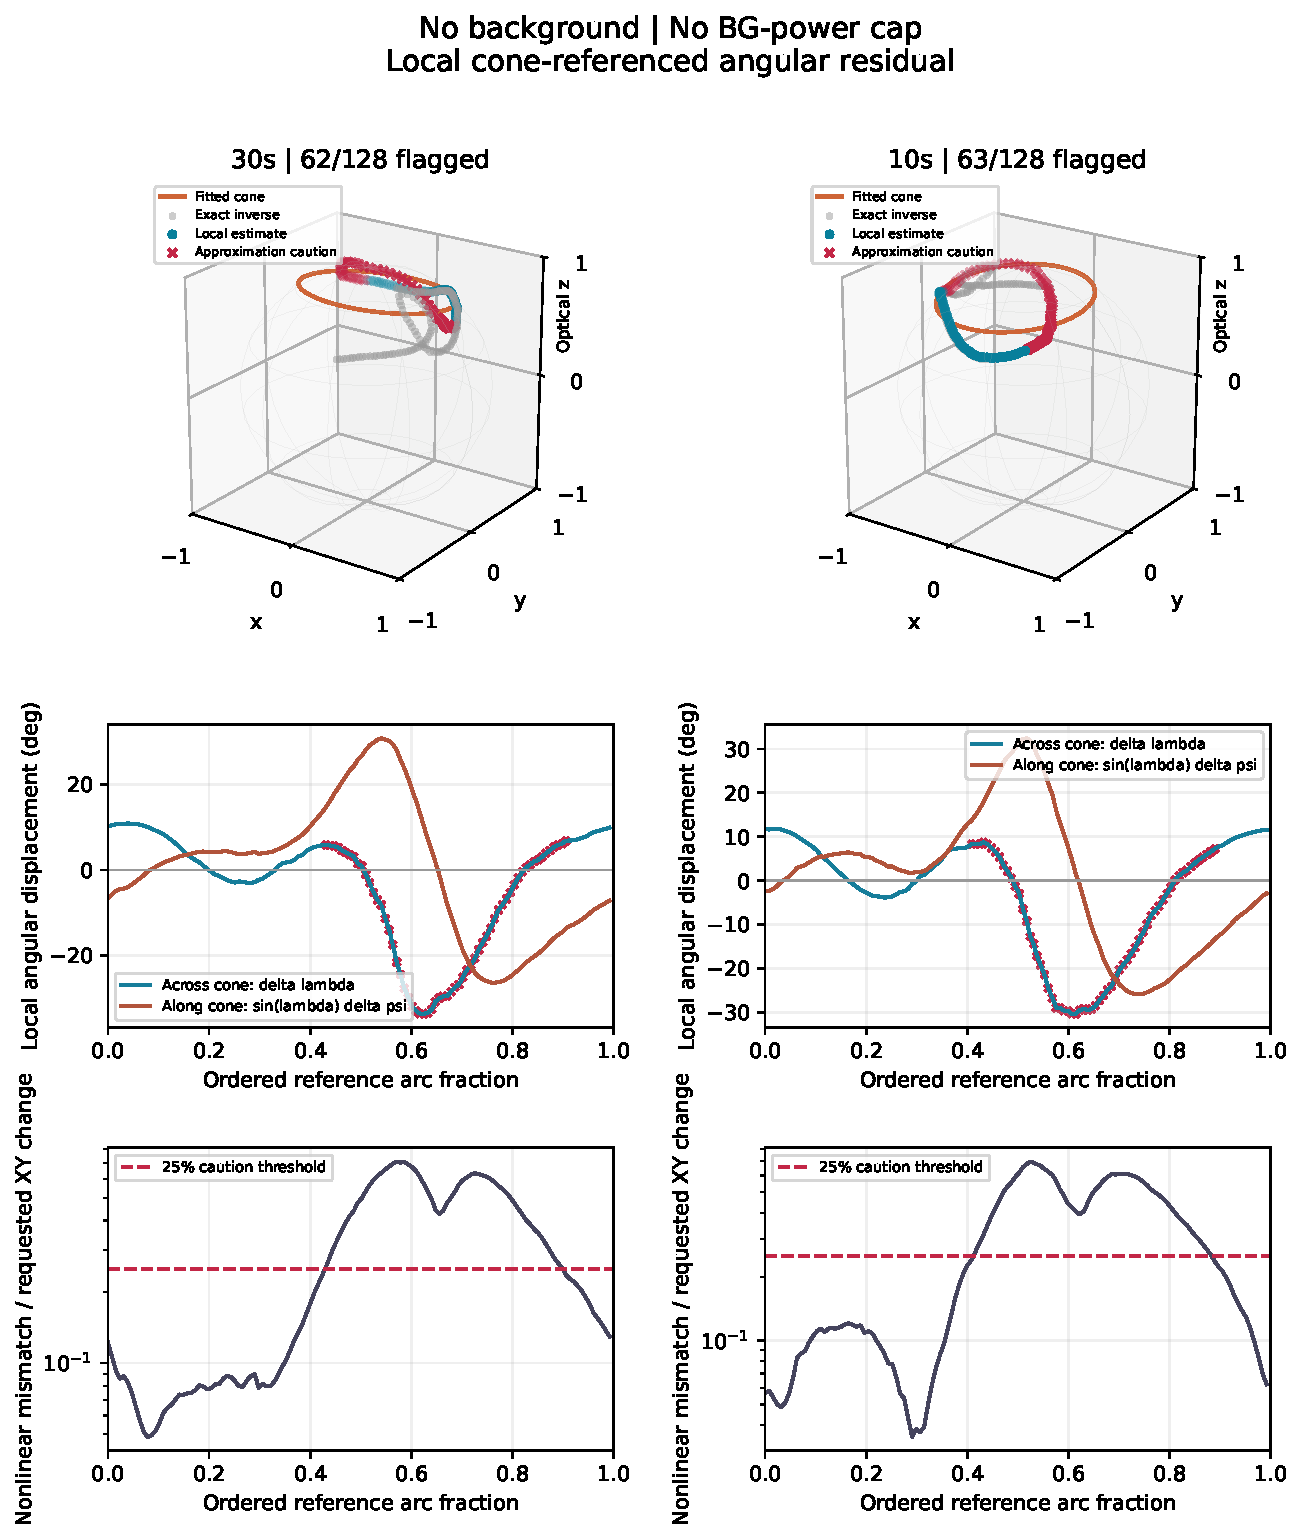
\includegraphics[width=\linewidth,height=.86\textheight,keepaspectratio]{local_residual/none.pdf}
30s: local angular RMS 20.58$^\circ$; 62/128 caution flags; median nonlinear mismatch ratio 0.224.\par
10s: local angular RMS 20.42$^\circ$; 63/128 caution flags; median nonlinear mismatch ratio 0.224.\par
\newpage
\section{Additive background}
\[I_i=S_i+B_i,\qquad T=T_S+B_{tot}.\]
\[\mathbf B=\frac{B_{tot}}4(1+f_x,1-f_x,1+f_y,1-f_y),\quad |f_x|,|f_y|\leq1.\]
Fit five cone/brightness/offset parameters plus $B_{tot},f_x,f_y$ separately per window. The background is constant, nonnegative and has equal pair sums. No Stokes-disk restriction is imposed, matching the recovered notebook form. Its coherent versus noninterfering composition is not identifiable because no cross term is modelled.
\textbf{Total fitted continuous parameters across both windows: 16.} The three pre-estimated gain adjustments are additional calibration parameters, held fixed here.
\begin{longtable}{llrrrrrr}\toprule
Budget & Window & BG\% & Meas.RMS & Signal RMS & Bad(train/test) & Max $r$ & Conv.\\\midrule\endhead
uncapped & 30s & 27.8 & 0.0367 & 0.1135 & 20/25 & 0.959 & yes \\
uncapped & 10s & 30.1 & 0.0397 & 0.1093 & 15/22 & 0.955 & yes \\
5pct & 30s & 5.0 & 0.0705 & 0.2282 & 0/0 & 0.765 & yes \\
5pct & 10s & 5.0 & 0.0643 & 0.0839 & 0/0 & 0.744 & yes \\
10pct & 30s & 10.0 & 0.0538 & 0.0838 & 0/0 & 0.864 & yes \\
10pct & 10s & 10.0 & 0.0553 & 0.0784 & 0/0 & 0.834 & yes \\
20pct & 30s & 20.0 & 0.0422 & 0.0888 & 9/9 & 0.940 & yes \\
20pct & 10s & 20.0 & 0.0446 & 0.0783 & 7/4 & 0.930 & yes \\
\bottomrule\end{longtable}
\begin{longtable}{llrrrr}\toprule
Budget & Window & Signal\% range & Cross\% range & Noninterf.BG\% & Fitted folded $\theta$\\\midrule\endhead
uncapped & 30s & 11.3--65.3 & 0.0--0.0 & --- & 25.8--89.6$^\circ$ \\
uncapped & 10s & 14.5--61.3 & 0.0--0.0 & --- & 30.5--89.8$^\circ$ \\
5pct & 30s & 10.8--86.4 & 0.0--0.0 & --- & 21.8--89.8$^\circ$ \\
5pct & 10s & 47.1--99.3 & 0.0--0.0 & --- & 32.1--49.3$^\circ$ \\
10pct & 30s & 30.4--96.5 & 0.0--0.0 & --- & 29.4--58.2$^\circ$ \\
10pct & 10s & 39.3--93.4 & 0.0--0.0 & --- & 32.5--54.1$^\circ$ \\
20pct & 30s & 20.1--79.8 & 0.0--0.0 & --- & 30.1--74.3$^\circ$ \\
20pct & 10s & 28.5--79.6 & 0.0--0.0 & --- & 34.1--65.5$^\circ$ \\
\bottomrule\end{longtable}
\textbf{Per-channel constant background, percent of measured maximum:}
\begin{longtable}{llrrrr}\toprule
Budget & Window & $B_0$ & $B_{90}$ & $B_{45}$ & $B_{135}$\\\midrule\endhead
uncapped & 30s & 6.95 & 6.96 & 4.78 & 9.12\\
uncapped & 10s & 7.43 & 7.61 & 4.80 & 10.23\\
5pct & 30s & 2.50 & 0.00 & 0.00 & 2.50\\
5pct & 10s & 2.50 & 0.00 & 0.00 & 2.50\\
10pct & 30s & 5.00 & 0.00 & 0.00 & 5.00\\
10pct & 10s & 5.00 & 0.00 & 0.00 & 5.00\\
20pct & 30s & 6.53 & 3.47 & 1.57 & 8.43\\
20pct & 10s & 6.96 & 3.04 & 0.98 & 9.02\\
\bottomrule\end{longtable}
\newpage
\subsection{No BG-power cap}\label{case:square:uncapped}
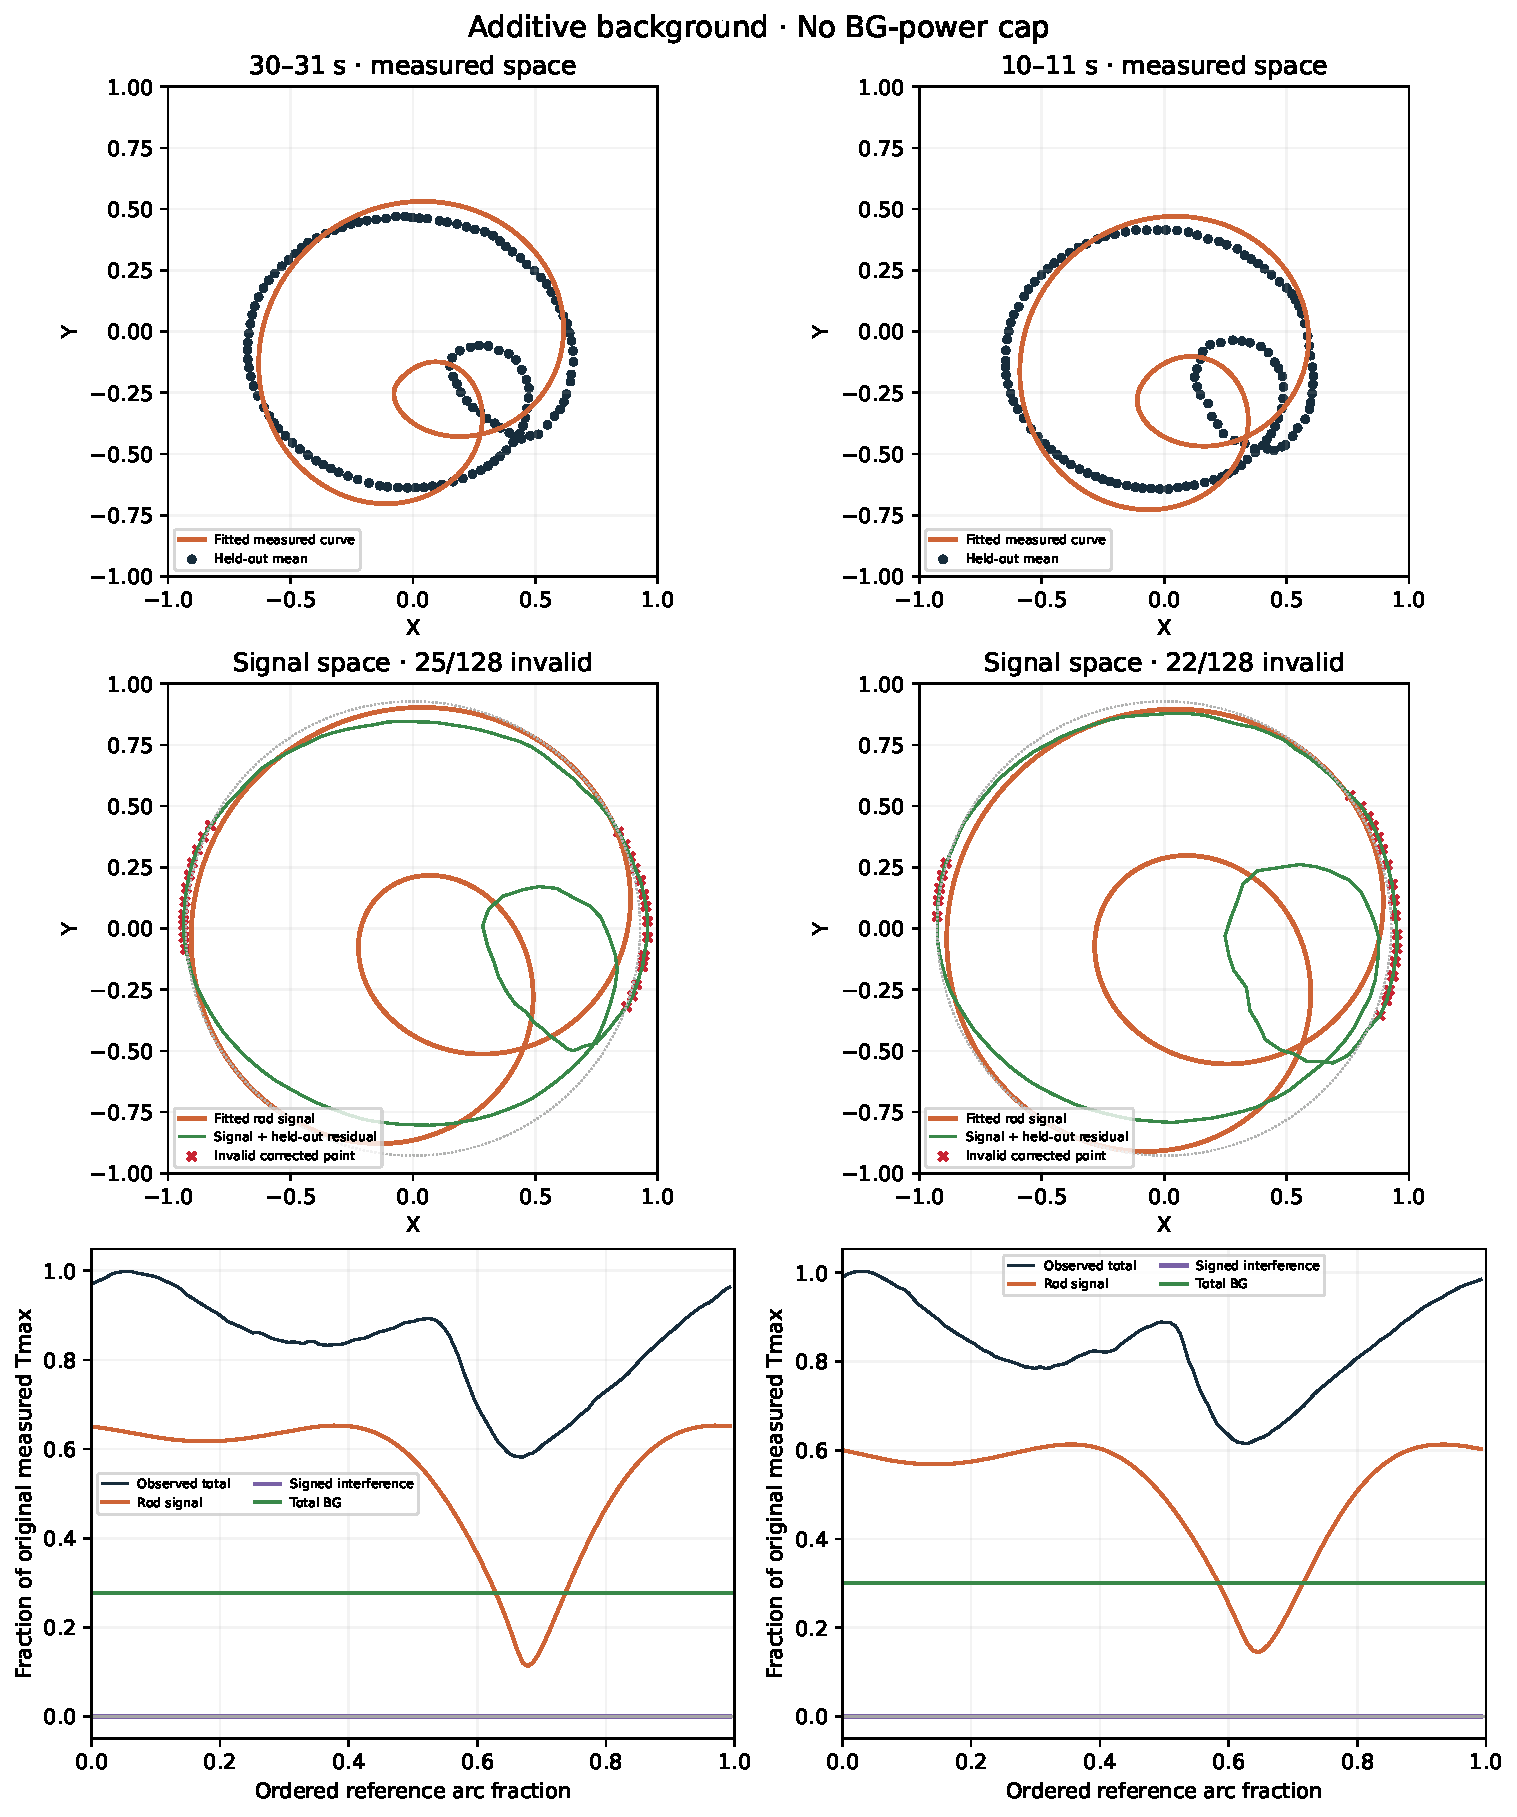
\includegraphics[width=\linewidth,height=.9\textheight,keepaspectratio]{figures/square_uncapped.pdf}
\newpage
\subsection{5\% of maximum}\label{case:square:5pct}
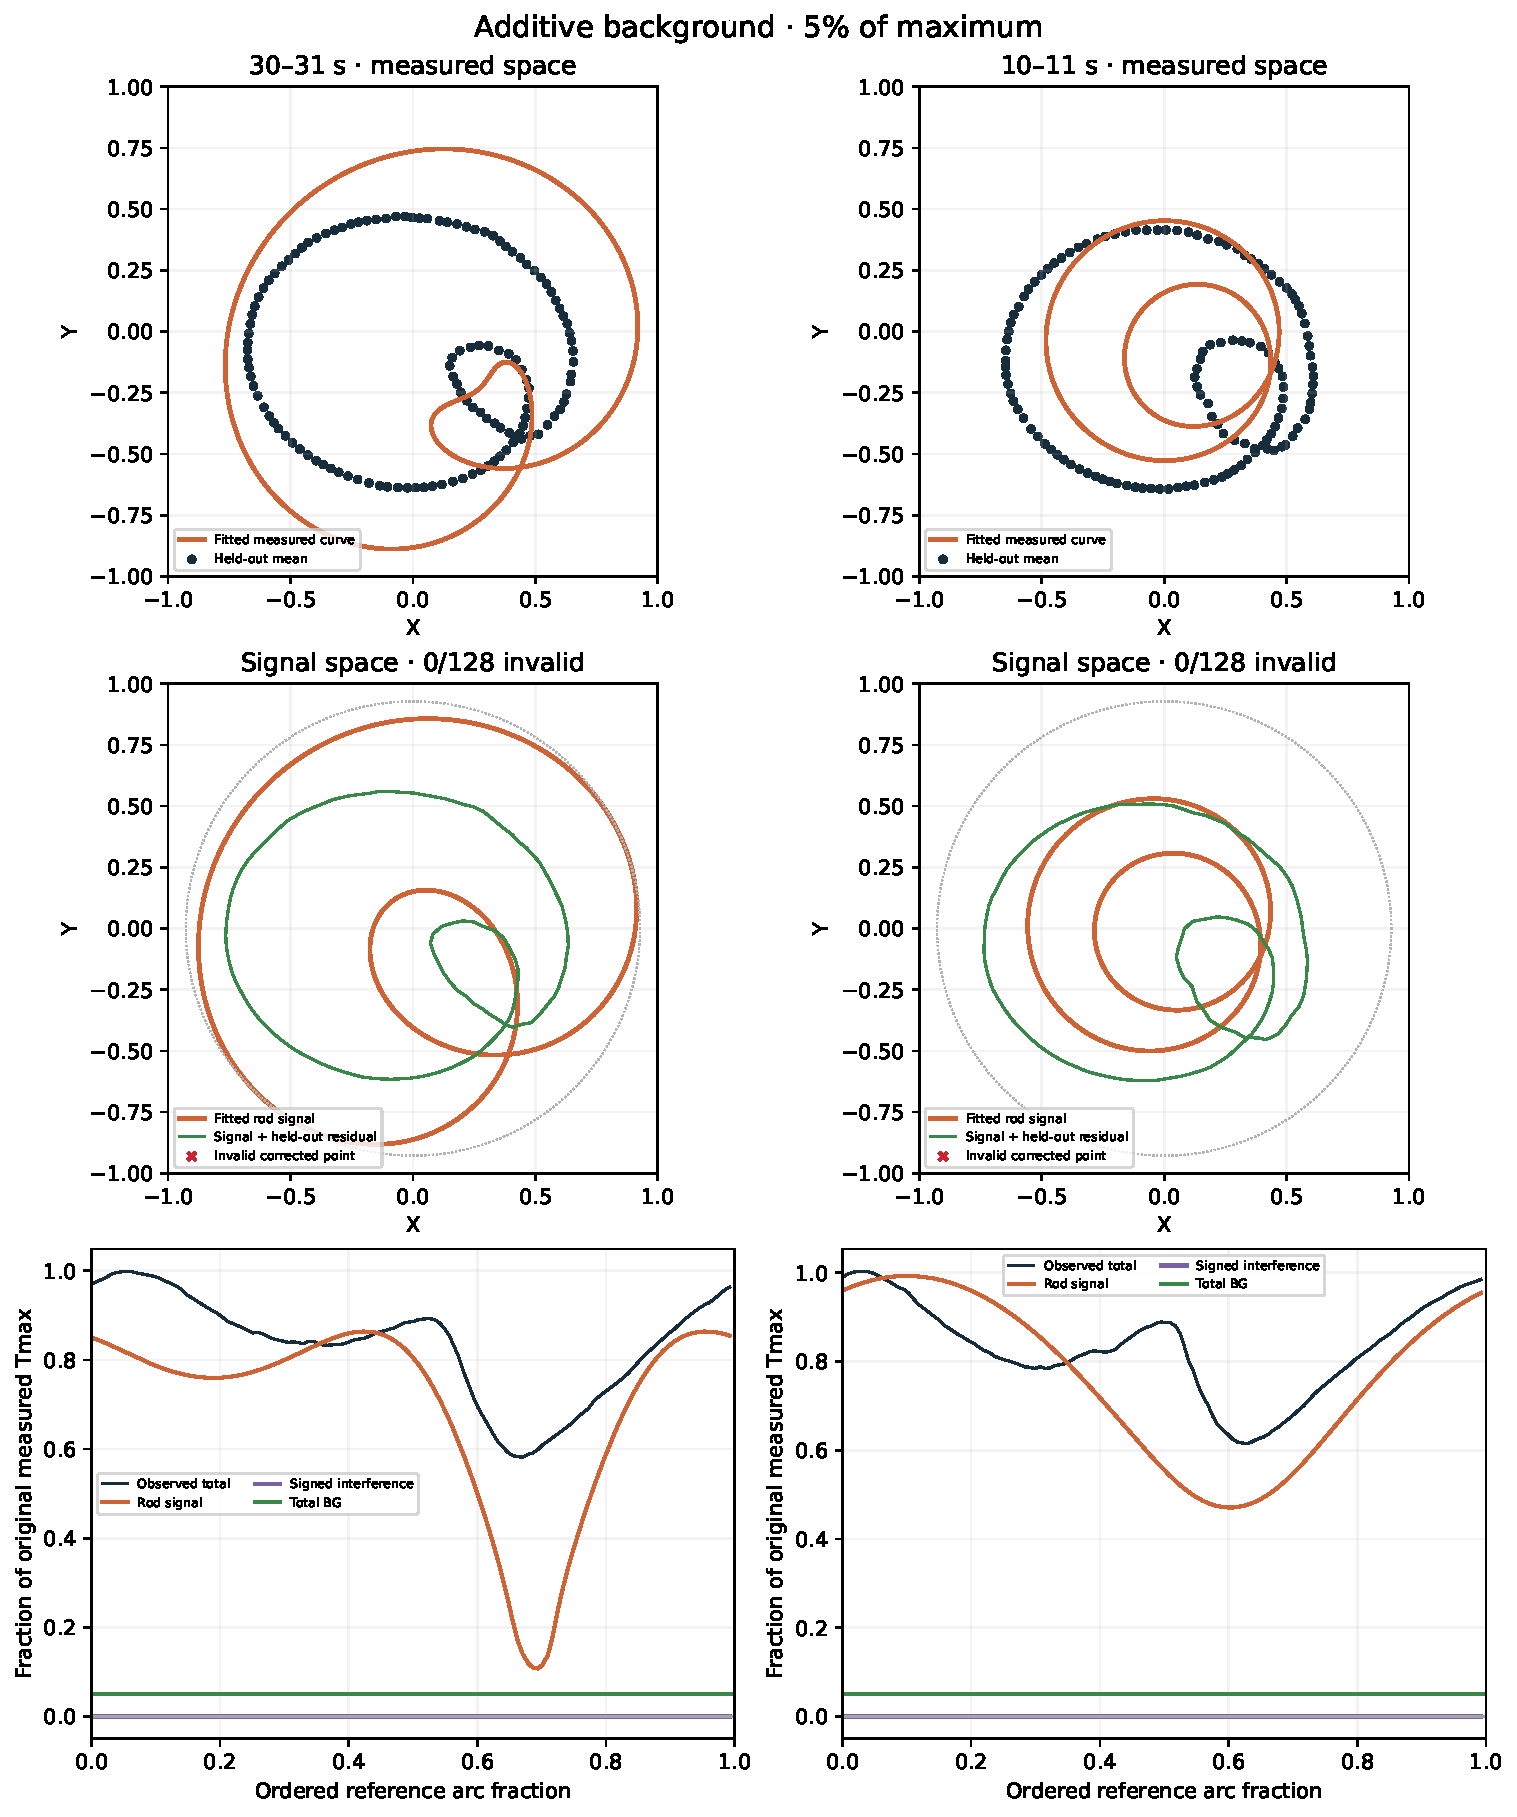
\includegraphics[width=\linewidth,height=.9\textheight,keepaspectratio]{figures/square_5pct.pdf}
\newpage
\subsection{10\% of maximum}\label{case:square:10pct}
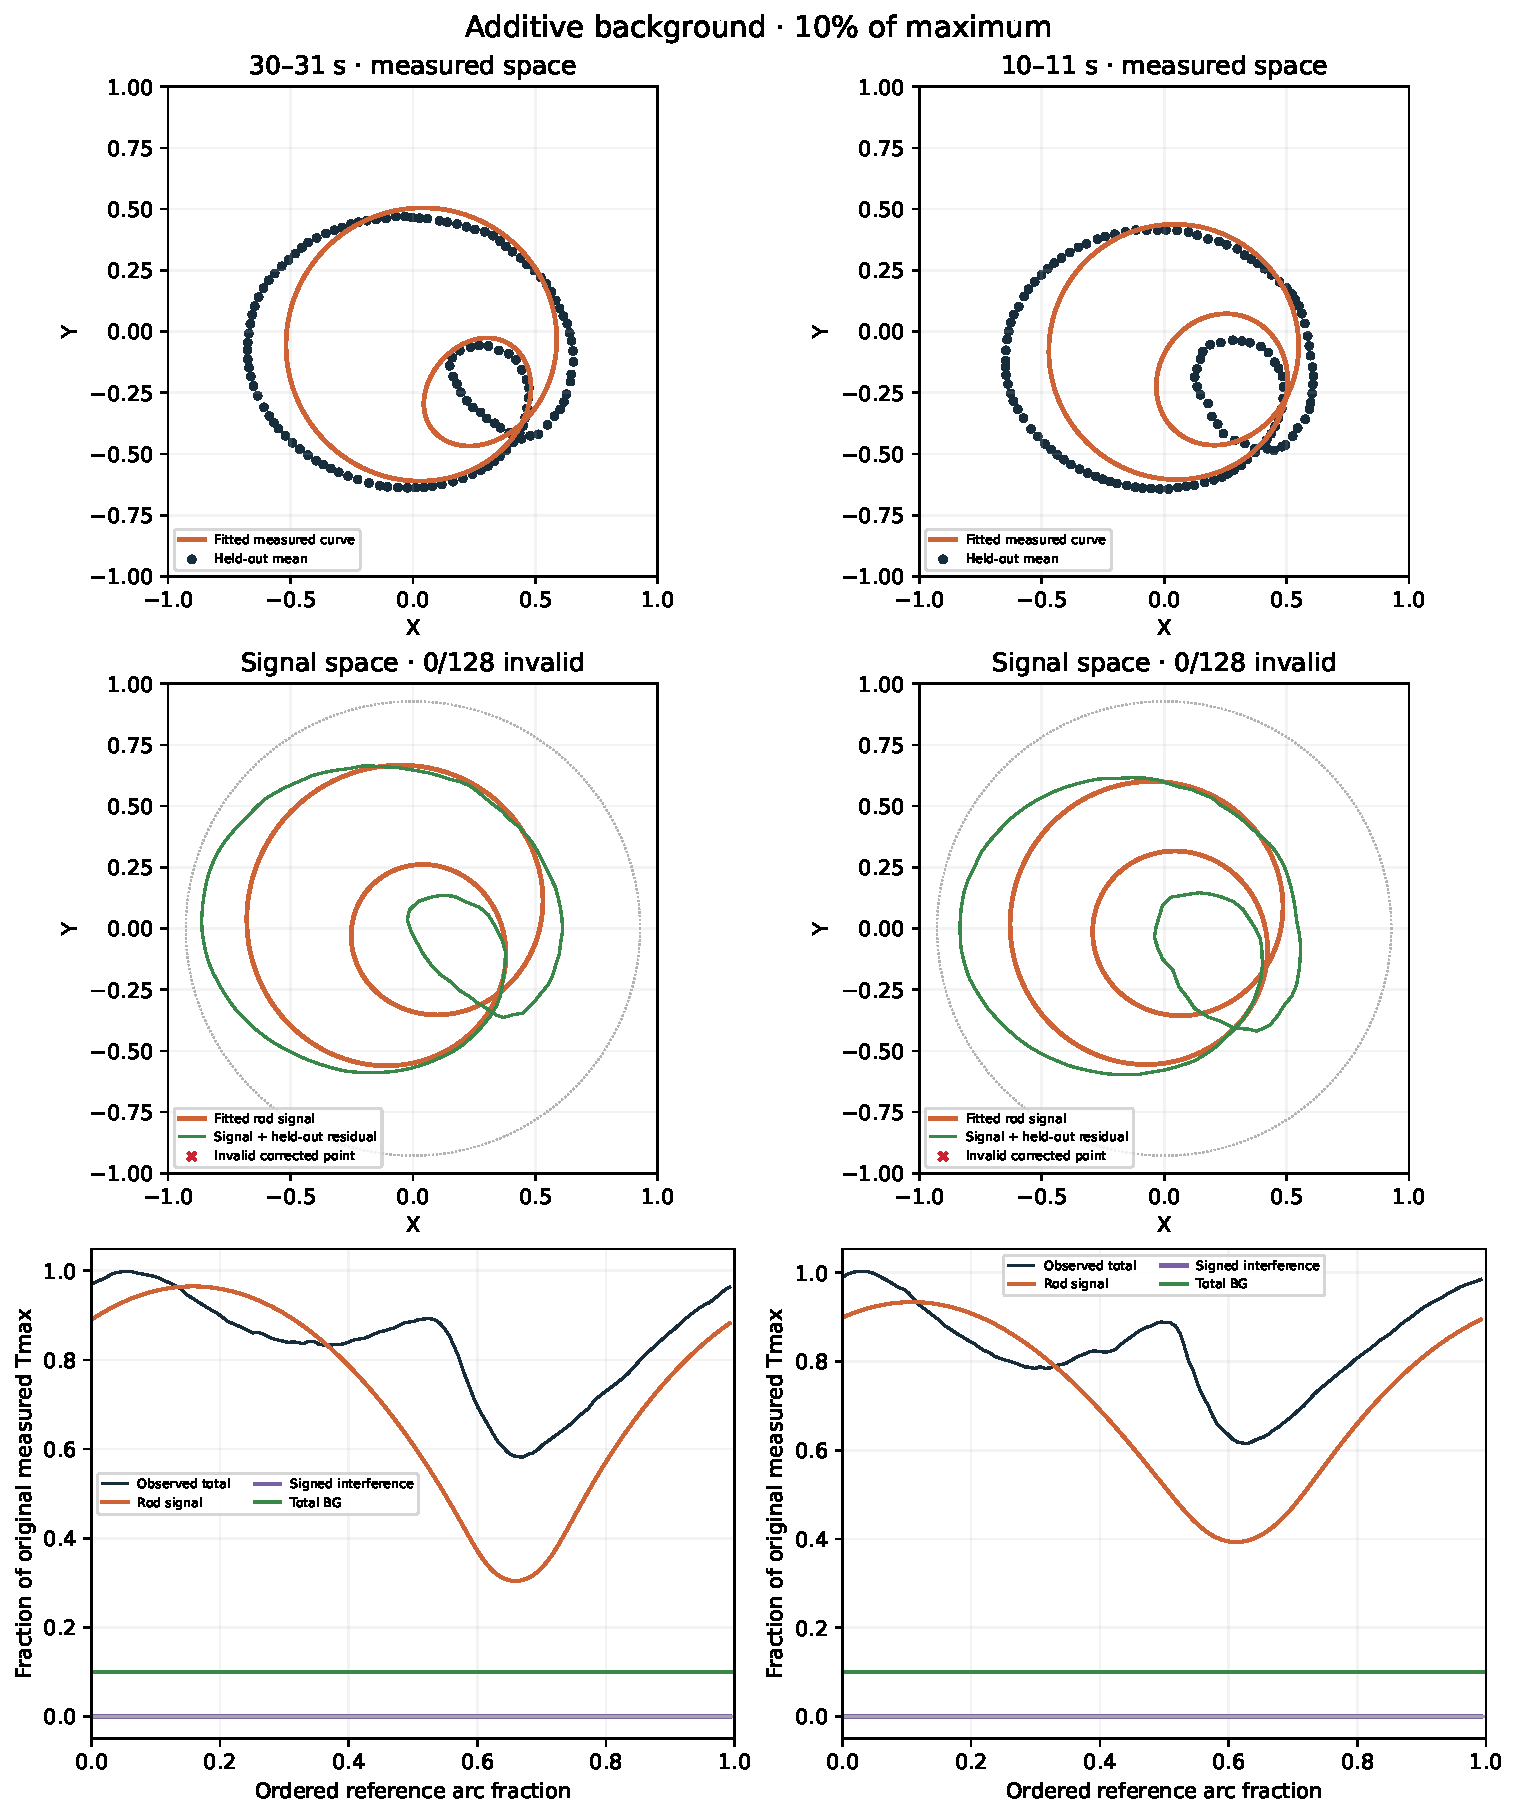
\includegraphics[width=\linewidth,height=.9\textheight,keepaspectratio]{figures/square_10pct.pdf}
\newpage
\subsection{20\% of maximum}\label{case:square:20pct}
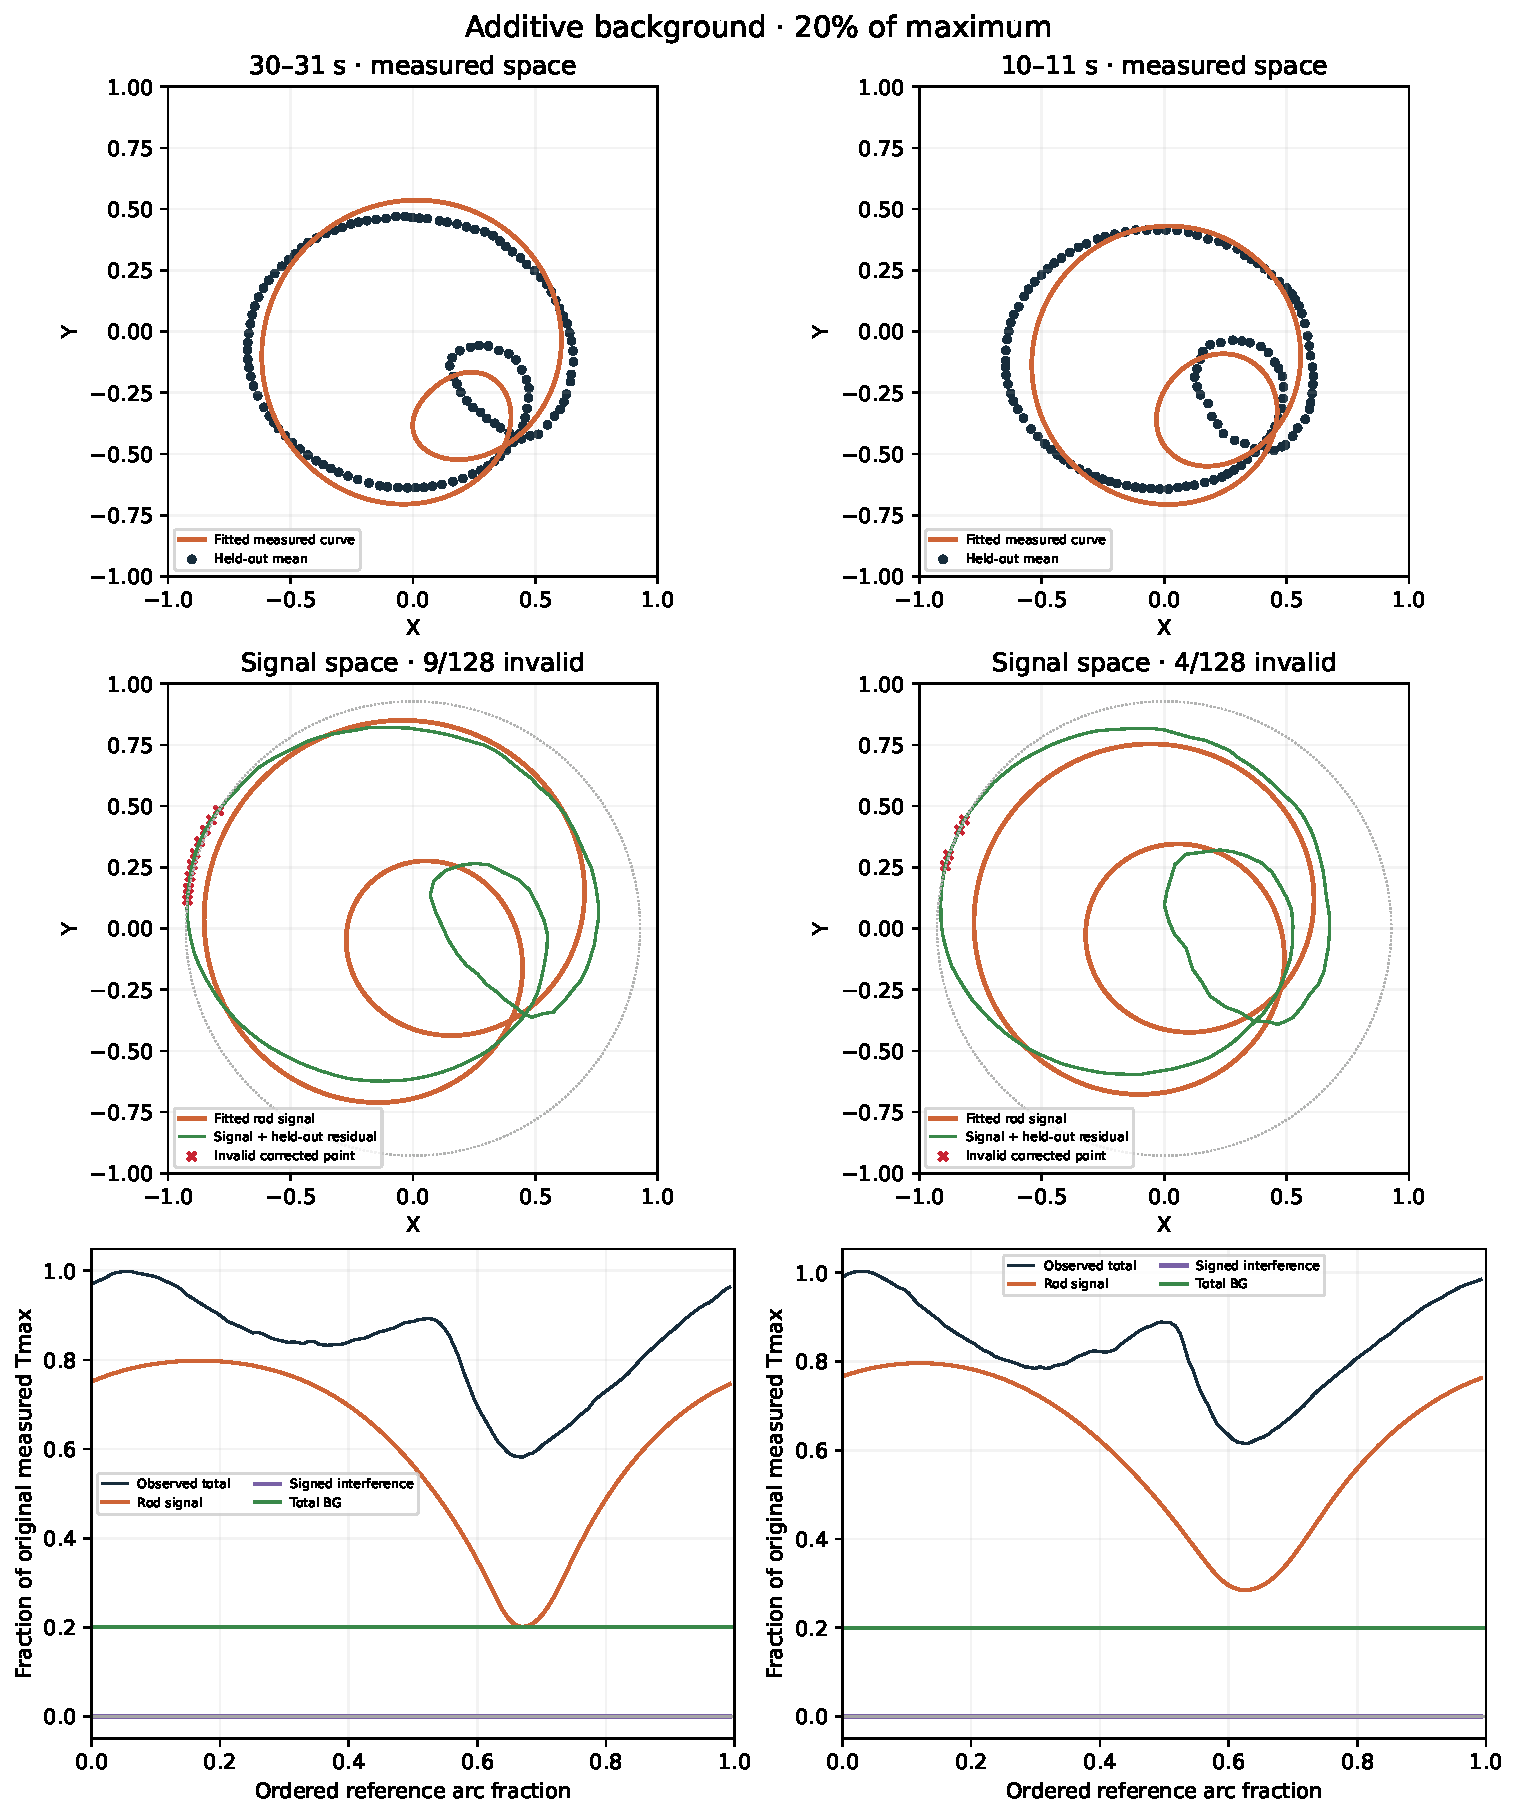
\includegraphics[width=\linewidth,height=.9\textheight,keepaspectratio]{figures/square_20pct.pdf}
\newpage
\subsection{Representative sphere diagnostic: 10\% of maximum}
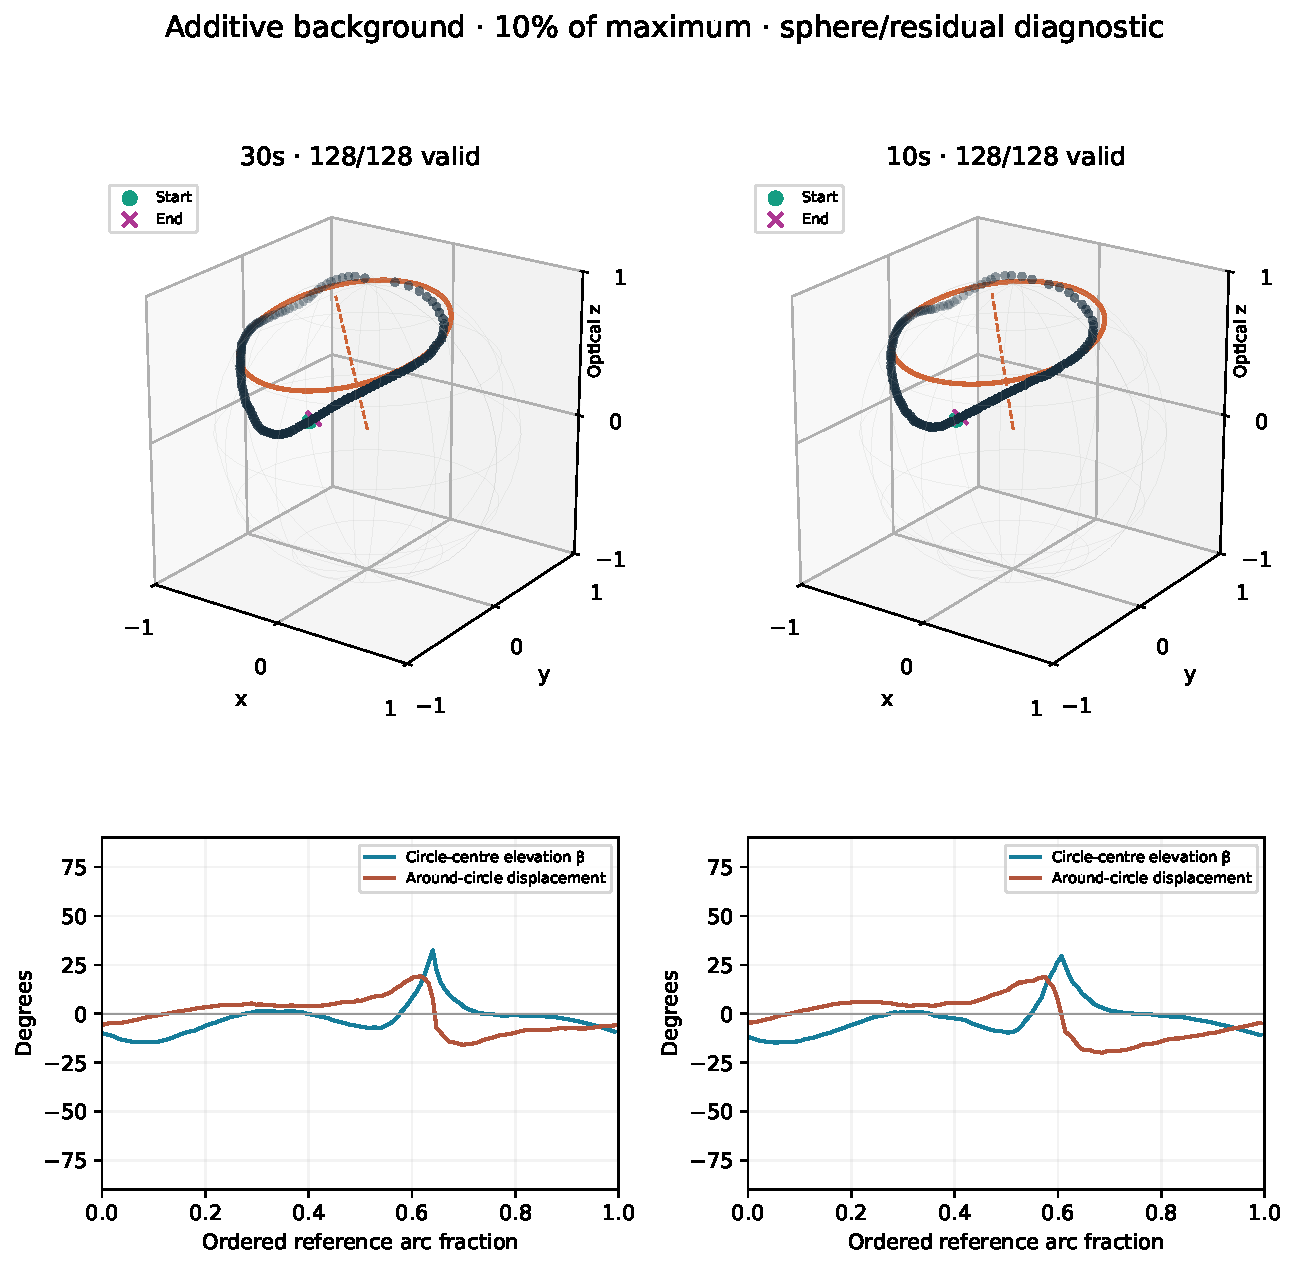
\includegraphics[width=\linewidth,height=.82\textheight,keepaspectratio]{figures/square_sphere.pdf}
30s: 128/128 valid; matched geodesic RMS 11.65$^\circ$; oriented closure mismatch 0.00$^\circ$.\par
10s: 128/128 valid; matched geodesic RMS 13.78$^\circ$; oriented closure mismatch 0.00$^\circ$.\par
\newpage
\subsection{Local cone-referenced angular residual: 10\% of maximum}\label{local:square}
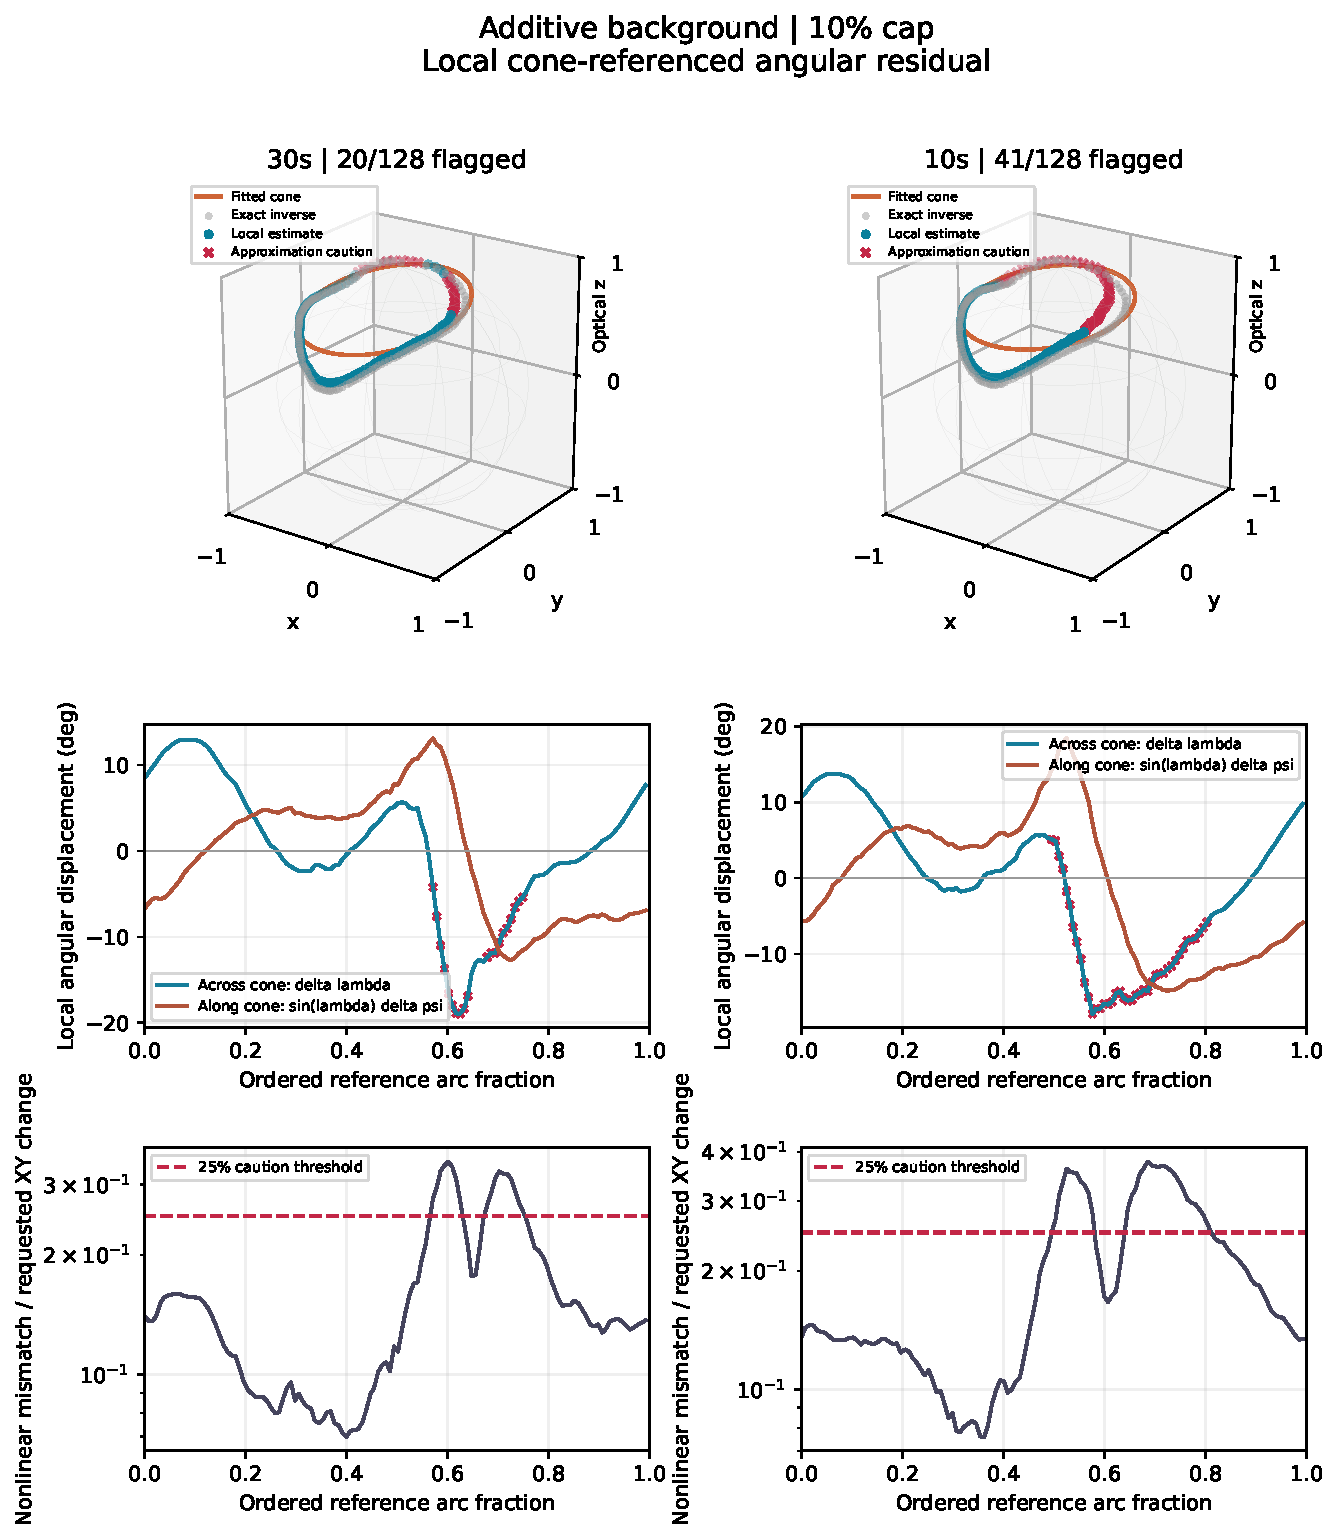
\includegraphics[width=\linewidth,height=.86\textheight,keepaspectratio]{local_residual/square.pdf}
30s: local angular RMS 10.58$^\circ$; 20/128 caution flags; median nonlinear mismatch ratio 0.138.\par
10s: local angular RMS 12.96$^\circ$; 41/128 caution flags; median nonlinear mismatch ratio 0.151.\par
\newpage
\section{Richard four-C}
\[I_i=S_i+C_i\sqrt{S_i},\qquad T=T_S+\sum_iC_i\sqrt{S_i}.\]
Fit five cone/brightness/offset parameters plus four constant signed $C_i$ separately per window. This is Richard's exact proposed approximation, without an additive $B_i$. Numerical variables are $\alpha=a_0^2$ and $K_i=a_0C_i$, so $I_i=\alpha f_i+K_i\sqrt{f_i}$. A background-power cap is \emph{not defined}; imposing one on $C_i$ would change the model. The limit $\alpha\to0$, $C_i\to\infty$ can preserve the product term.

For uniform comparison the green curves and penalties here use frozen fitted cross-term subtraction $I^{obs}-C_i\sqrt{S_i^{fit}}$. This differs from the exact quadratic inverse used in an earlier sphere report. Four independent $C_i$ do not guarantee interference pair balance or a common physical background field.
\textbf{Total fitted continuous parameters across both windows: 18.} The three pre-estimated gain adjustments are additional calibration parameters, held fixed here.
\begin{longtable}{llrrrrrr}\toprule
Budget & Window & BG\% & Meas.RMS & Signal RMS & Bad(train/test) & Max $r$ & Conv.\\\midrule\endhead
uncapped & 30s & --- & 0.0463 & 0.2287 & 7/3 & 0.936 & yes \\
uncapped & 10s & --- & 0.0463 & 0.2281 & 6/14 & 0.980 & yes \\
\bottomrule\end{longtable}
\begin{longtable}{llrrrr}\toprule
Budget & Window & Signal\% range & Cross\% range & Noninterf.BG\% & Fitted folded $\theta$\\\midrule\endhead
uncapped & 30s & 8.6--36.0 & 30.5--60.5 & --- & 30.7--89.4$^\circ$ \\
uncapped & 10s & 9.5--30.9 & 35.9--64.1 & --- & 35.2--87.8$^\circ$ \\
\bottomrule\end{longtable}
\textbf{Per-channel constant background, percent of measured maximum:}
\begin{longtable}{llrrrr}\toprule
Budget & Window & $B_0$ & $B_{90}$ & $B_{45}$ & $B_{135}$\\\midrule\endhead
uncapped & 30s & 0.00 & 0.00 & 0.00 & 0.00\\
uncapped & 10s & 0.00 & 0.00 & 0.00 & 0.00\\
\bottomrule\end{longtable}
\textbf{Fitted effective coefficients (normalized intensity units):}\par
30s: $\alpha=0.089579$, $K_i=(0.1686,0.1492,0.1215,0.1933)$. Finite $C_i=K_i/\sqrt{\alpha}$.\par
10s: $\alpha=0.07749$, $K_i=(0.175,0.1518,0.1239,0.2134)$. Finite $C_i=K_i/\sqrt{\alpha}$.\par
\newpage
\subsection{No BG-power cap}\label{case:richard_product:uncapped}
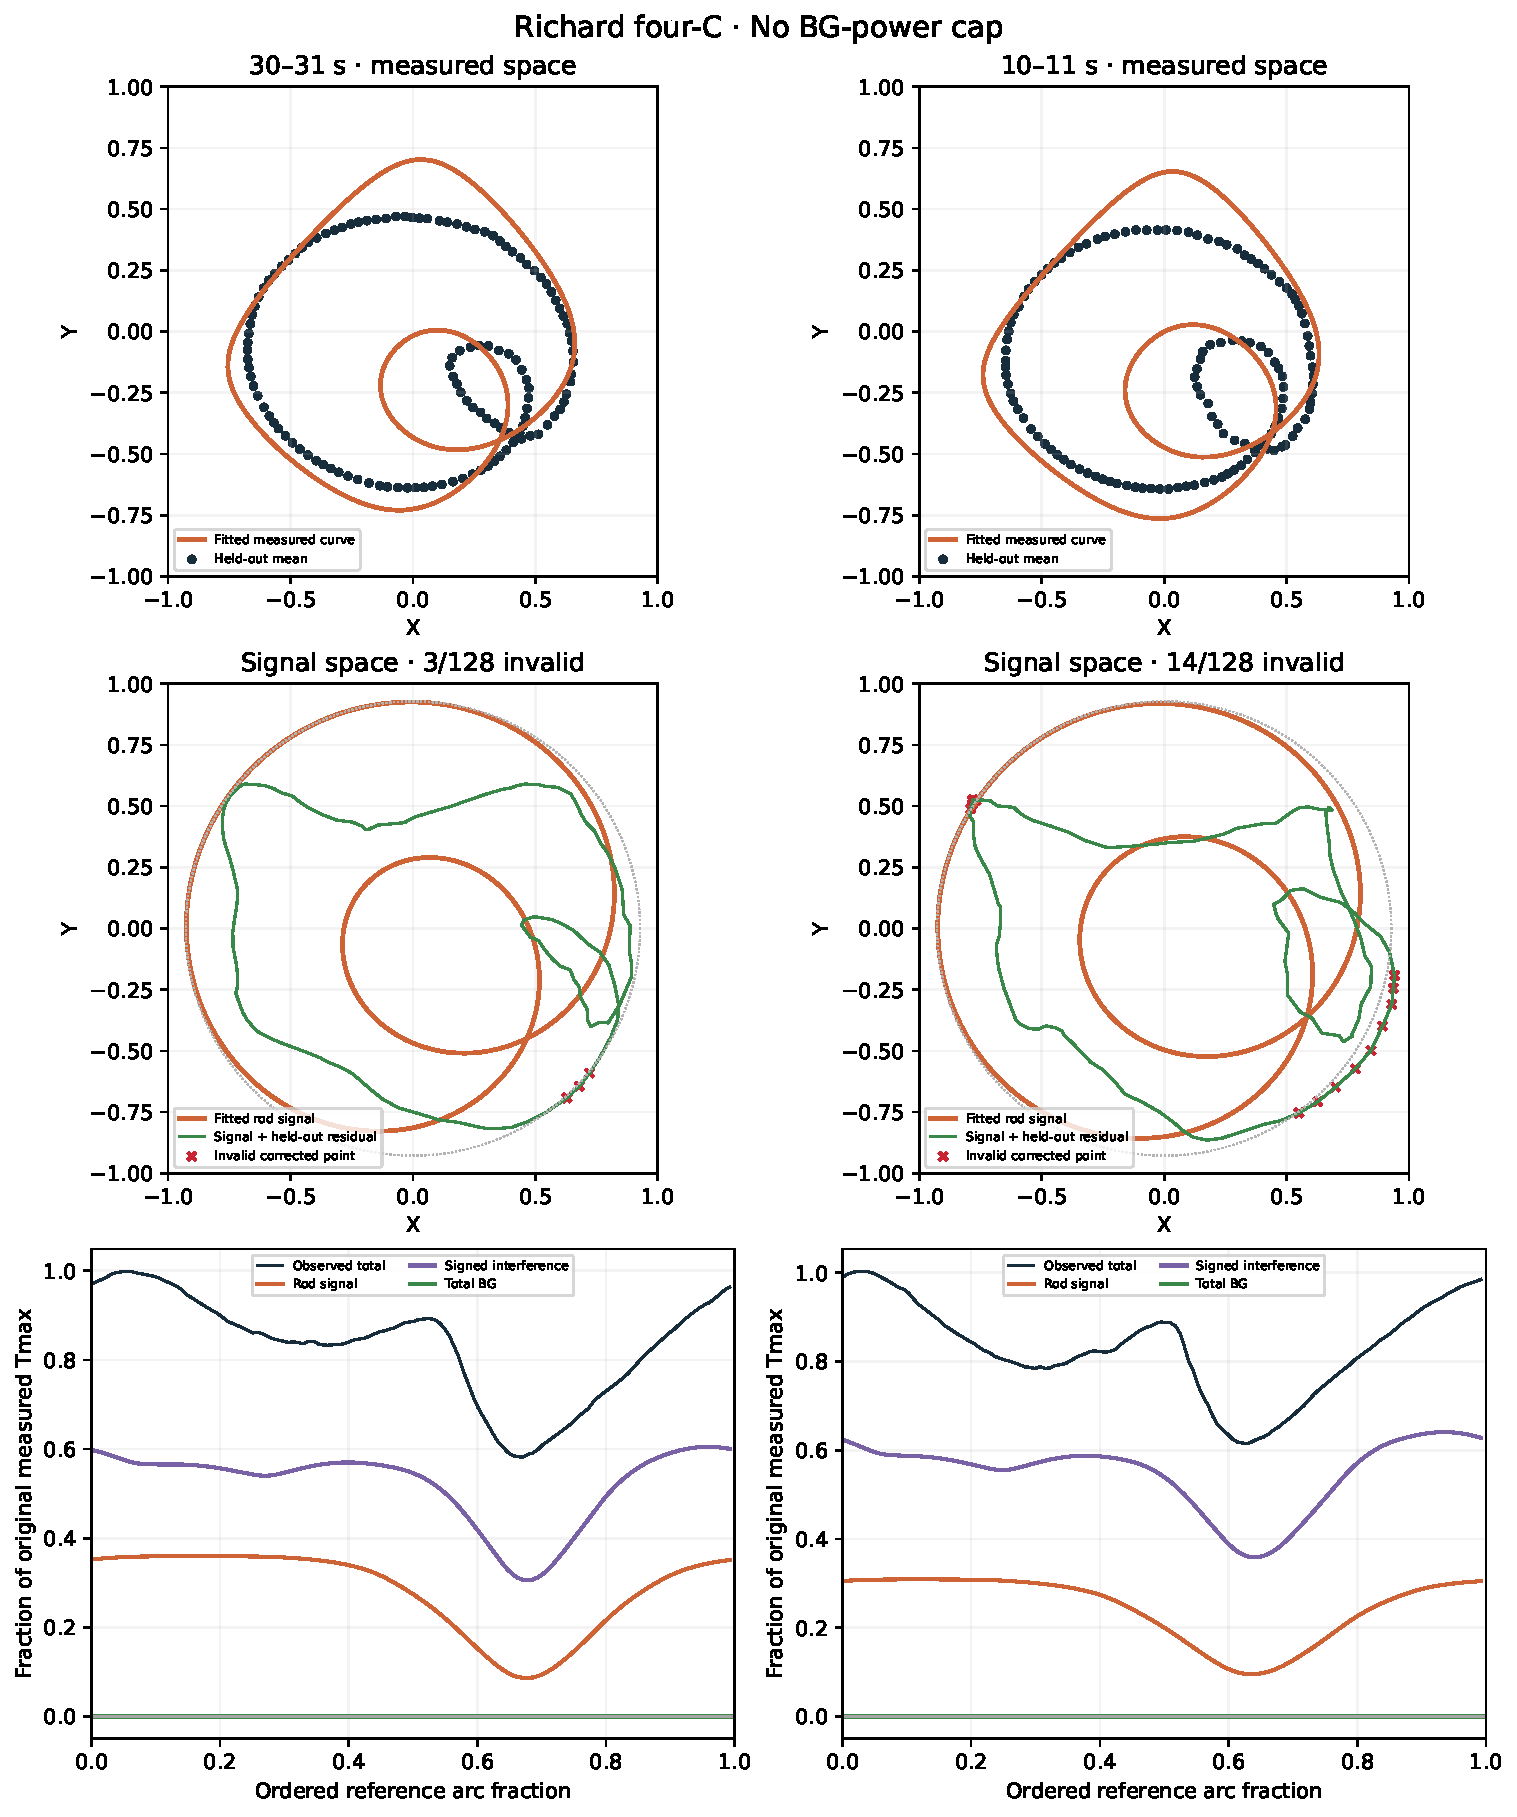
\includegraphics[width=\linewidth,height=.9\textheight,keepaspectratio]{figures/richard_product_uncapped.pdf}
\newpage
\subsection{Representative sphere diagnostic: No BG-power cap}
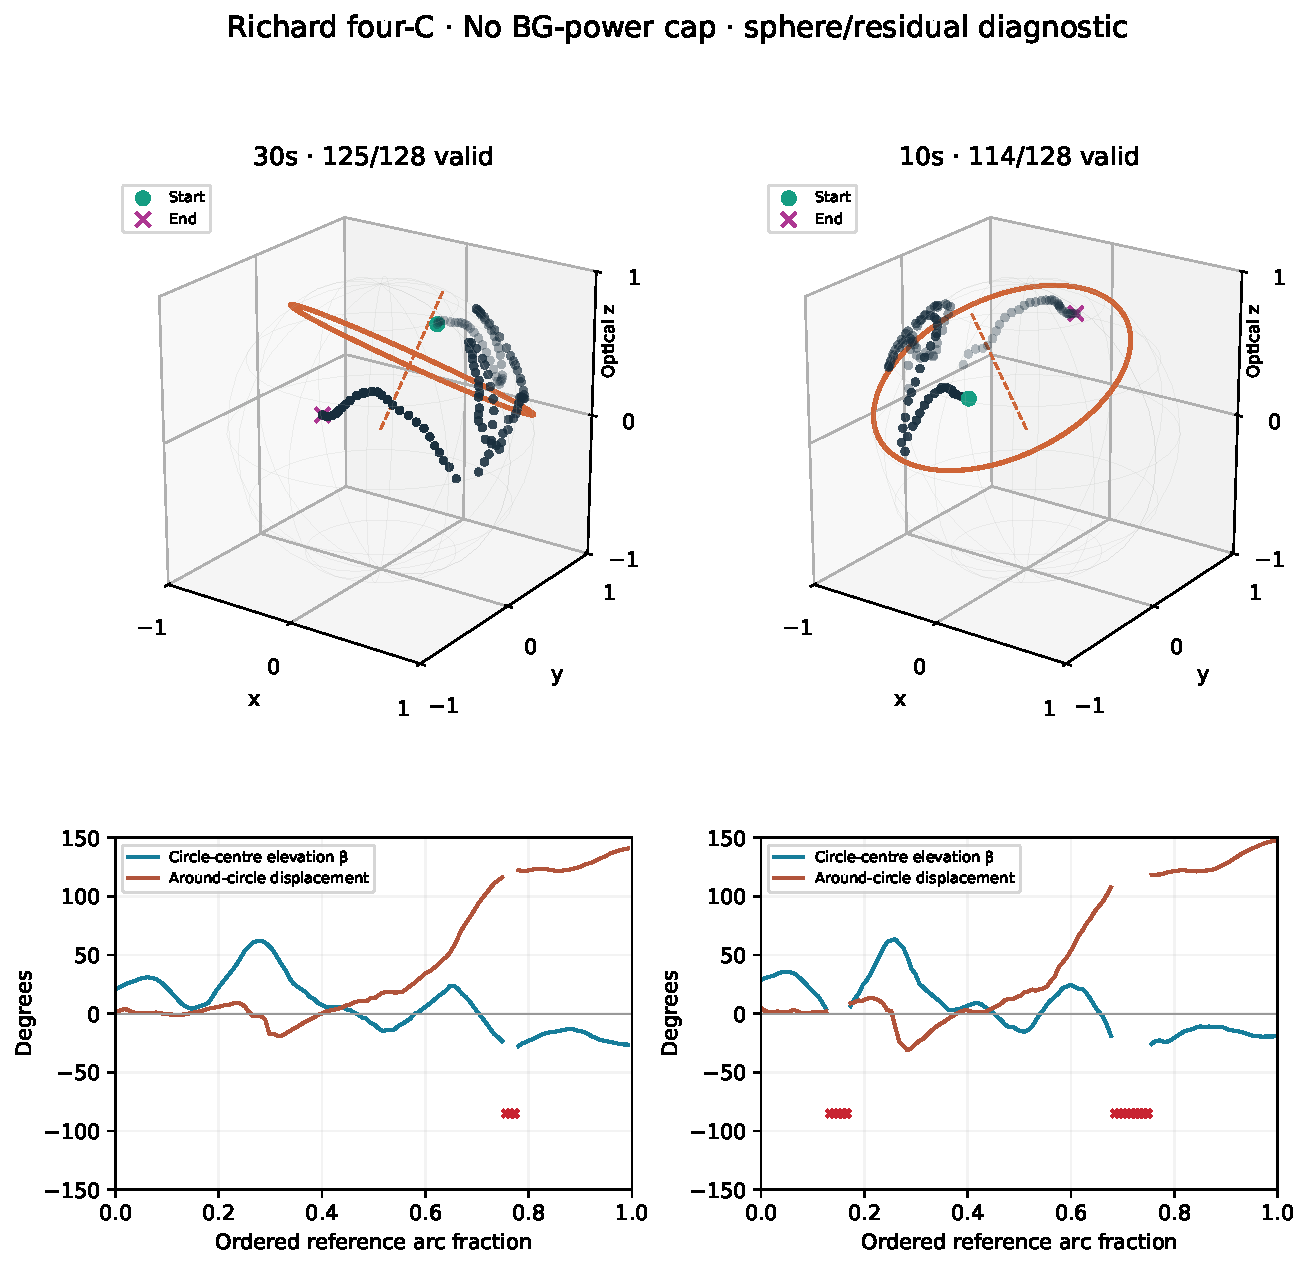
\includegraphics[width=\linewidth,height=.82\textheight,keepaspectratio]{figures/richard_product_sphere.pdf}
30s: 125/128 valid; matched geodesic RMS 71.88$^\circ$; closure unresolved (excluded bins); oriented endpoint mismatch 128.76$^\circ$.\par
10s: 114/128 valid; matched geodesic RMS 74.55$^\circ$; closure unresolved (excluded bins); oriented endpoint mismatch 117.48$^\circ$.\par
\newpage
\subsection{Local cone-referenced angular residual: No BG-power cap}\label{local:richard_product}
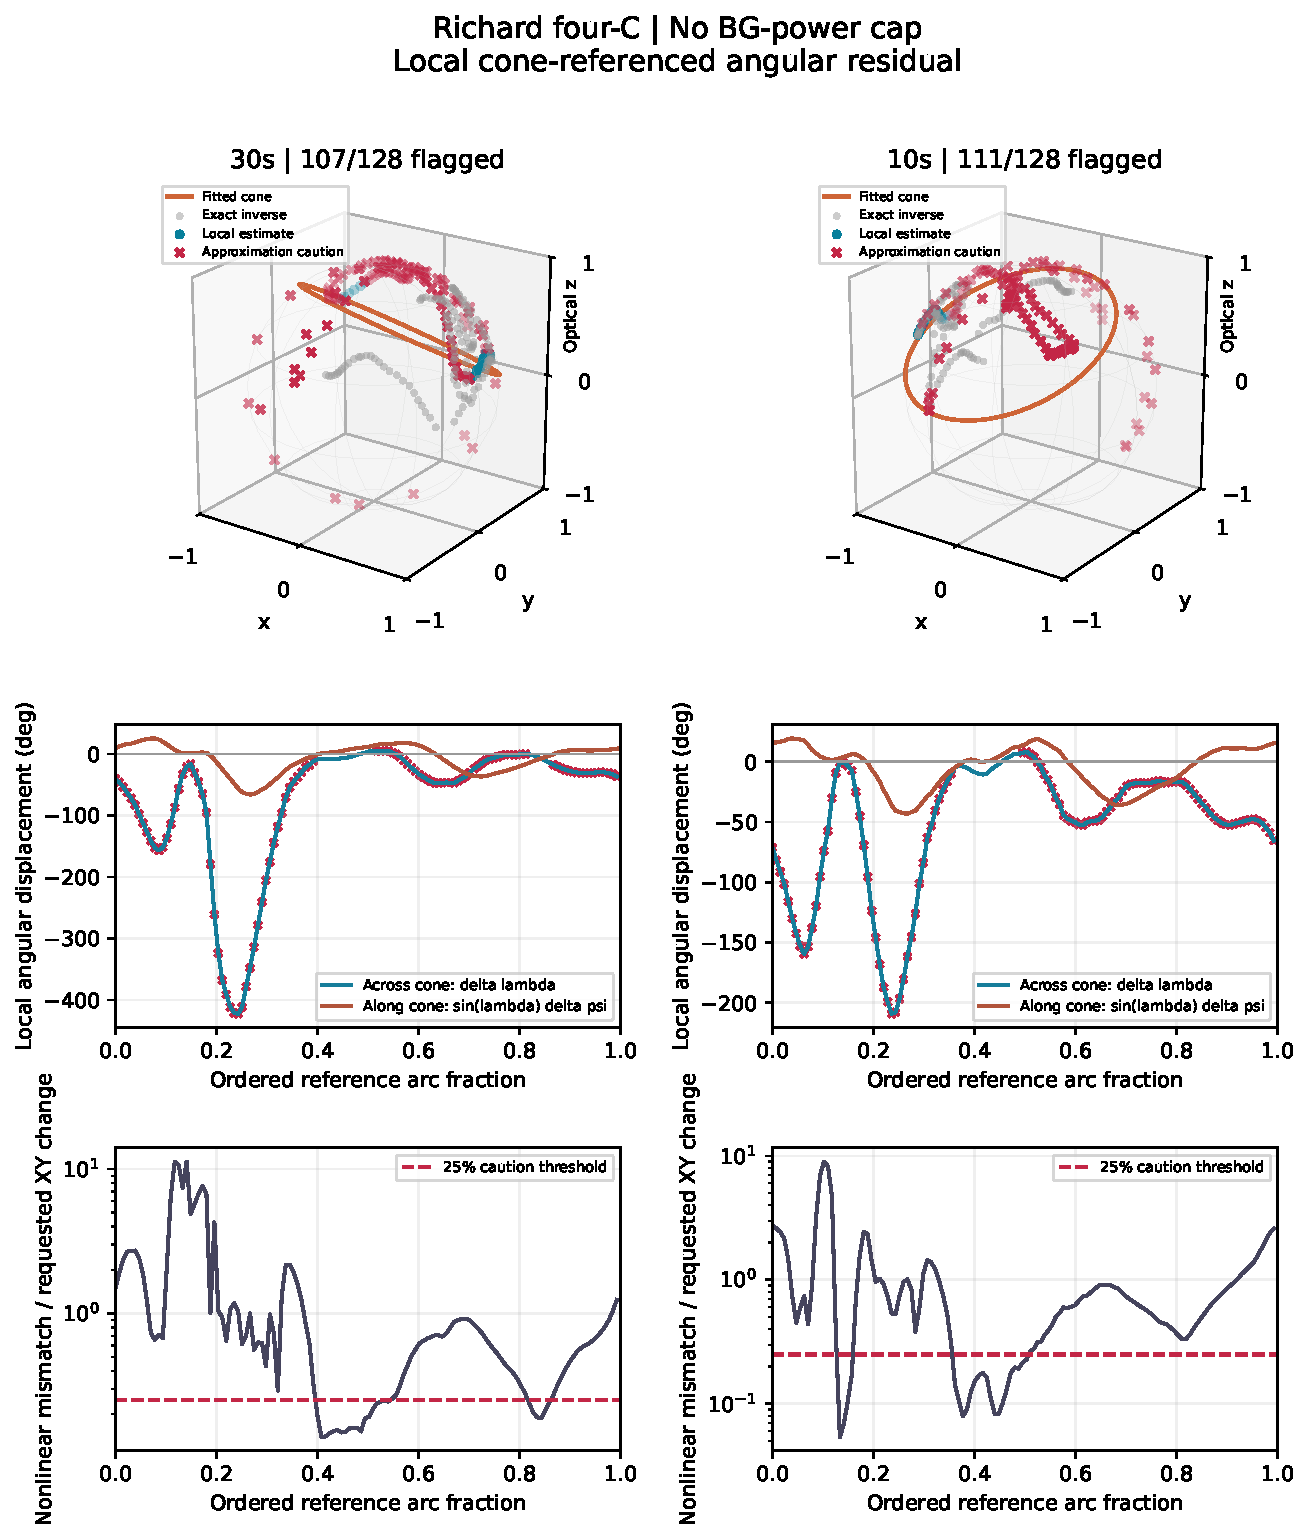
\includegraphics[width=\linewidth,height=.86\textheight,keepaspectratio]{local_residual/richard_product.pdf}
30s: local angular RMS 129.41$^\circ$; 107/128 caution flags; median nonlinear mismatch ratio 0.654.\par
10s: local angular RMS 76.39$^\circ$; 111/128 caution flags; median nonlinear mismatch ratio 0.624.\par
\newpage
\section{Additive plus bounded interference}
\[I_i=S_i+B_i+2\rho_i\sqrt{B_iS_i},\qquad |\rho_i|\leq1.\]
\[T=T_S+B_{tot}+2\sum_i\rho_i\sqrt{B_iS_i}.\]
Use the same three-parameter nonnegative equal-pair-sum additive background as above, plus four constant overlap coefficients $\rho_i$. Fit these seven correction parameters and five cone/brightness/offset parameters per window. Each channel obeys a scalar interference bound. This alone does not establish a realizable common pupil field or interference pair balance. $B_i$ is the represented available background power; its coherent/noninterfering split is not separately inferred.
\textbf{Total fitted continuous parameters across both windows: 24.} The three pre-estimated gain adjustments are additional calibration parameters, held fixed here.
\begin{longtable}{llrrrrrr}\toprule
Budget & Window & BG\% & Meas.RMS & Signal RMS & Bad(train/test) & Max $r$ & Conv.\\\midrule\endhead
uncapped & 30s & 88.5 & 0.0292 & 0.0200 & 6/8 & 0.939 & yes \\
uncapped & 10s & 90.8 & 0.0319 & 0.0225 & 6/5 & 0.935 & yes \\
5pct & 30s & 5.0 & 0.0482 & 0.1286 & 5/4 & 0.933 & yes \\
5pct & 10s & 5.0 & 0.0491 & 0.1107 & 6/4 & 0.933 & yes \\
10pct & 30s & 10.0 & 0.0415 & 0.1647 & 5/2 & 0.930 & yes \\
10pct & 10s & 10.0 & 0.0436 & 0.1473 & 4/5 & 0.934 & yes \\
\bottomrule\end{longtable}
\begin{longtable}{llrrrr}\toprule
Budget & Window & Signal\% range & Cross\% range & Noninterf.BG\% & Fitted folded $\theta$\\\midrule\endhead
uncapped & 30s & 54.5--167.2 & -158.1---92.1 & --- & 32.3--65.2$^\circ$ \\
uncapped & 10s & 65.7--159.0 & -155.2---100.7 & --- & 36.3--63.9$^\circ$ \\
5pct & 30s & 16.7--63.8 & 16.9--32.1 & --- & 30.9--75.2$^\circ$ \\
5pct & 10s & 22.9--63.8 & 18.7--31.9 & --- & 34.9--67.9$^\circ$ \\
10pct & 30s & 10.2--47.3 & 18.1--37.7 & --- & 29.1--89.9$^\circ$ \\
10pct & 10s & 13.8--44.7 & 22.2--39.8 & --- & 35.2--88.1$^\circ$ \\
\bottomrule\end{longtable}
\textbf{Per-channel constant background, percent of measured maximum:}
\begin{longtable}{llrrrr}\toprule
Budget & Window & $B_0$ & $B_{90}$ & $B_{45}$ & $B_{135}$\\\midrule\endhead
uncapped & 30s & 25.18 & 19.07 & 23.73 & 20.52\\
uncapped & 10s & 26.20 & 19.22 & 24.98 & 20.44\\
5pct & 30s & 1.71 & 0.79 & 0.37 & 2.13\\
5pct & 10s & 1.80 & 0.70 & 0.26 & 2.24\\
10pct & 30s & 3.02 & 1.98 & 1.34 & 3.66\\
10pct & 10s & 2.88 & 2.12 & 1.21 & 3.79\\
\bottomrule\end{longtable}
\newpage
\subsection{No BG-power cap}\label{case:complex:uncapped}
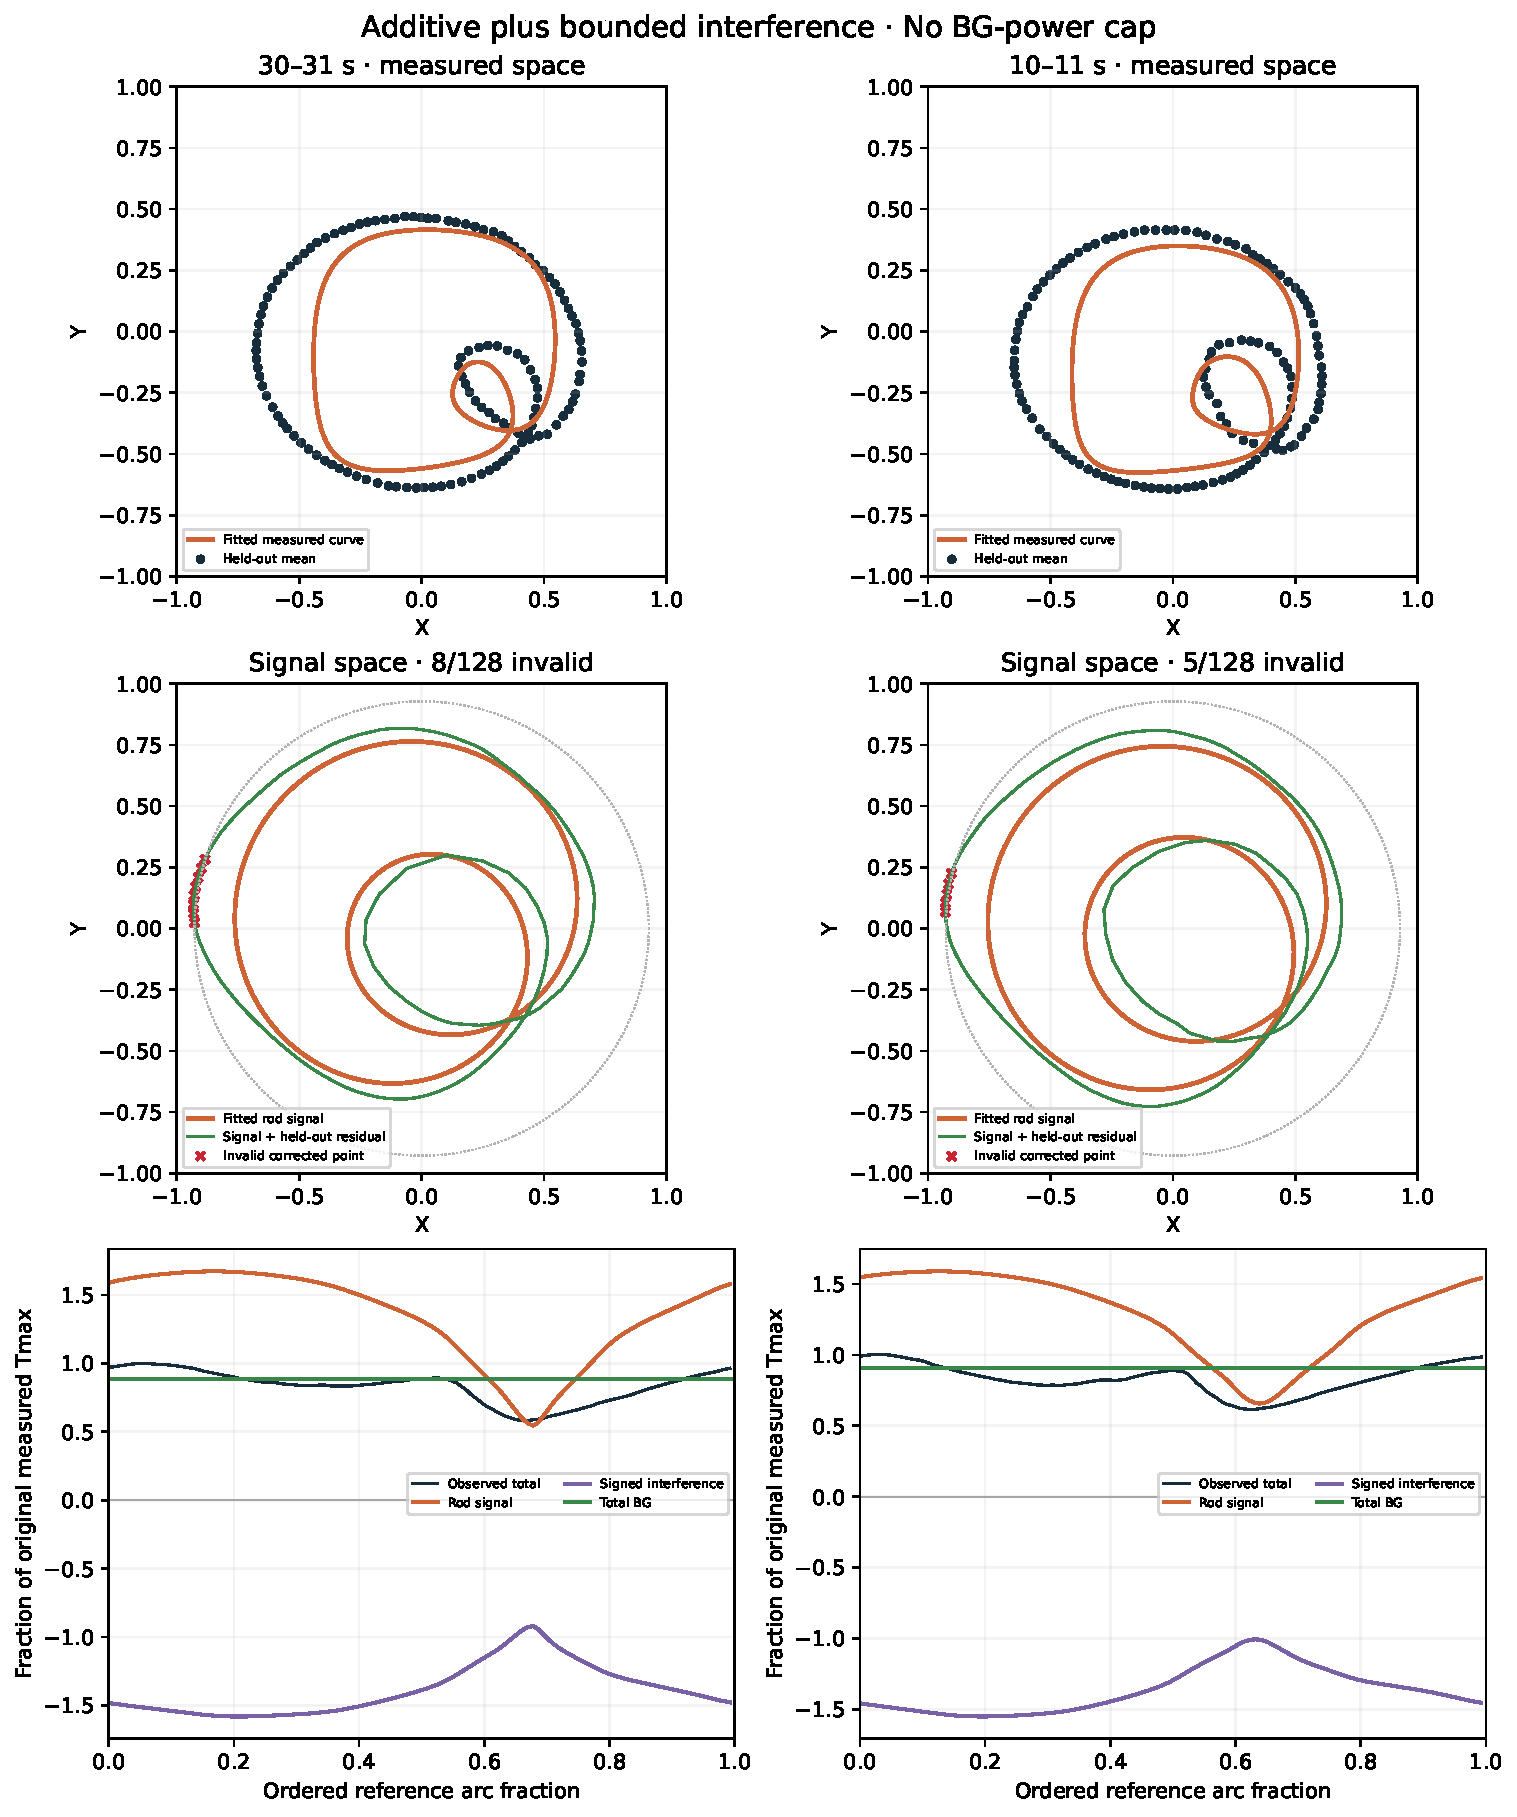
\includegraphics[width=\linewidth,height=.9\textheight,keepaspectratio]{figures/complex_uncapped.pdf}
\newpage
\subsection{5\% of maximum}\label{case:complex:5pct}
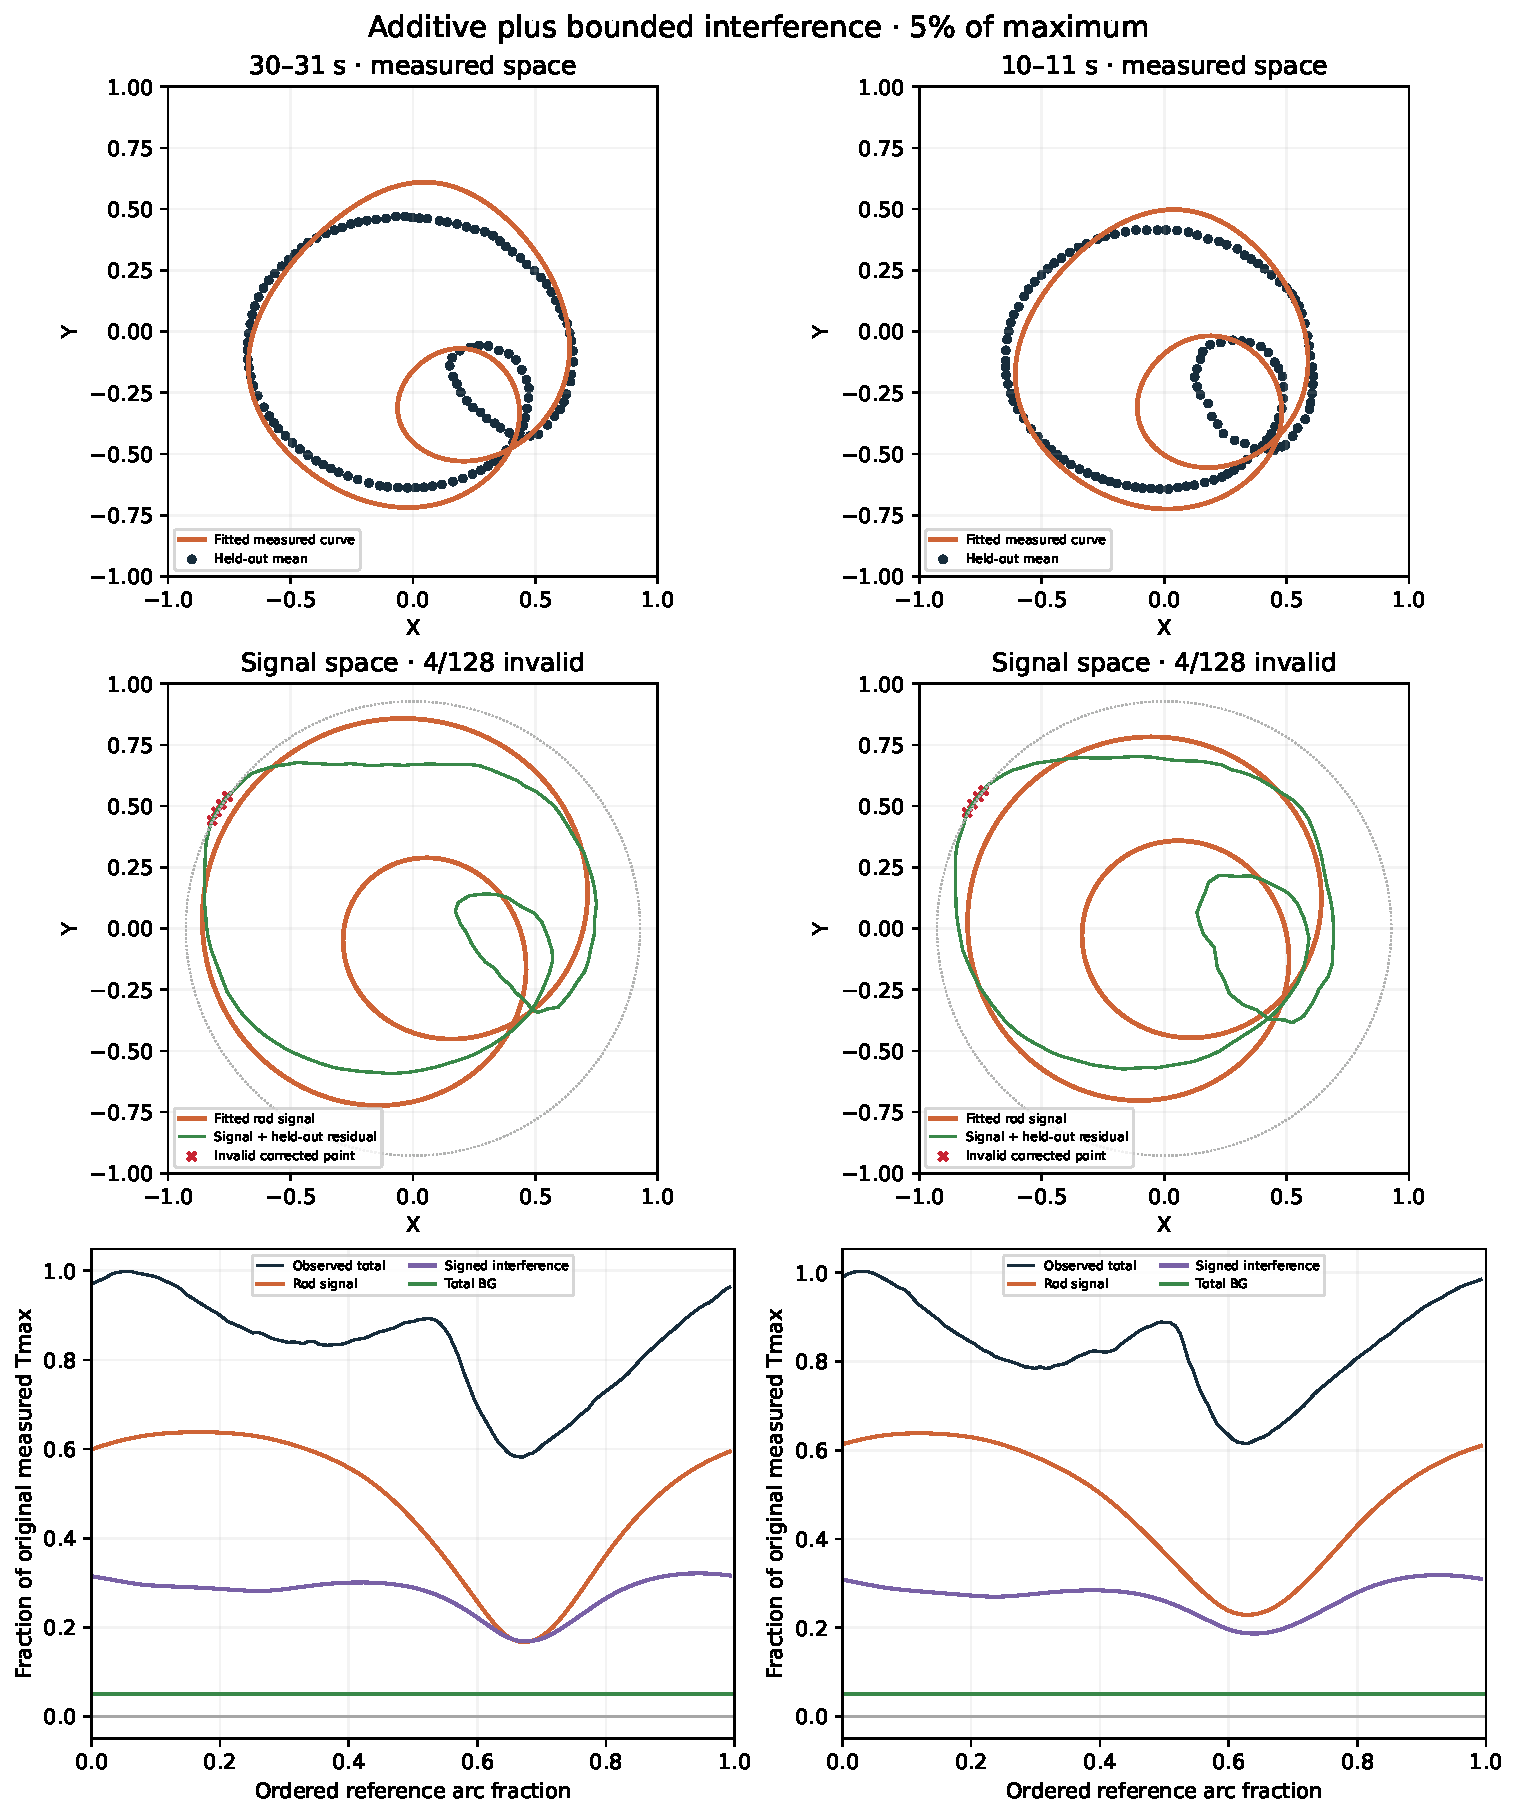
\includegraphics[width=\linewidth,height=.9\textheight,keepaspectratio]{figures/complex_5pct.pdf}
\newpage
\subsection{10\% of maximum}\label{case:complex:10pct}
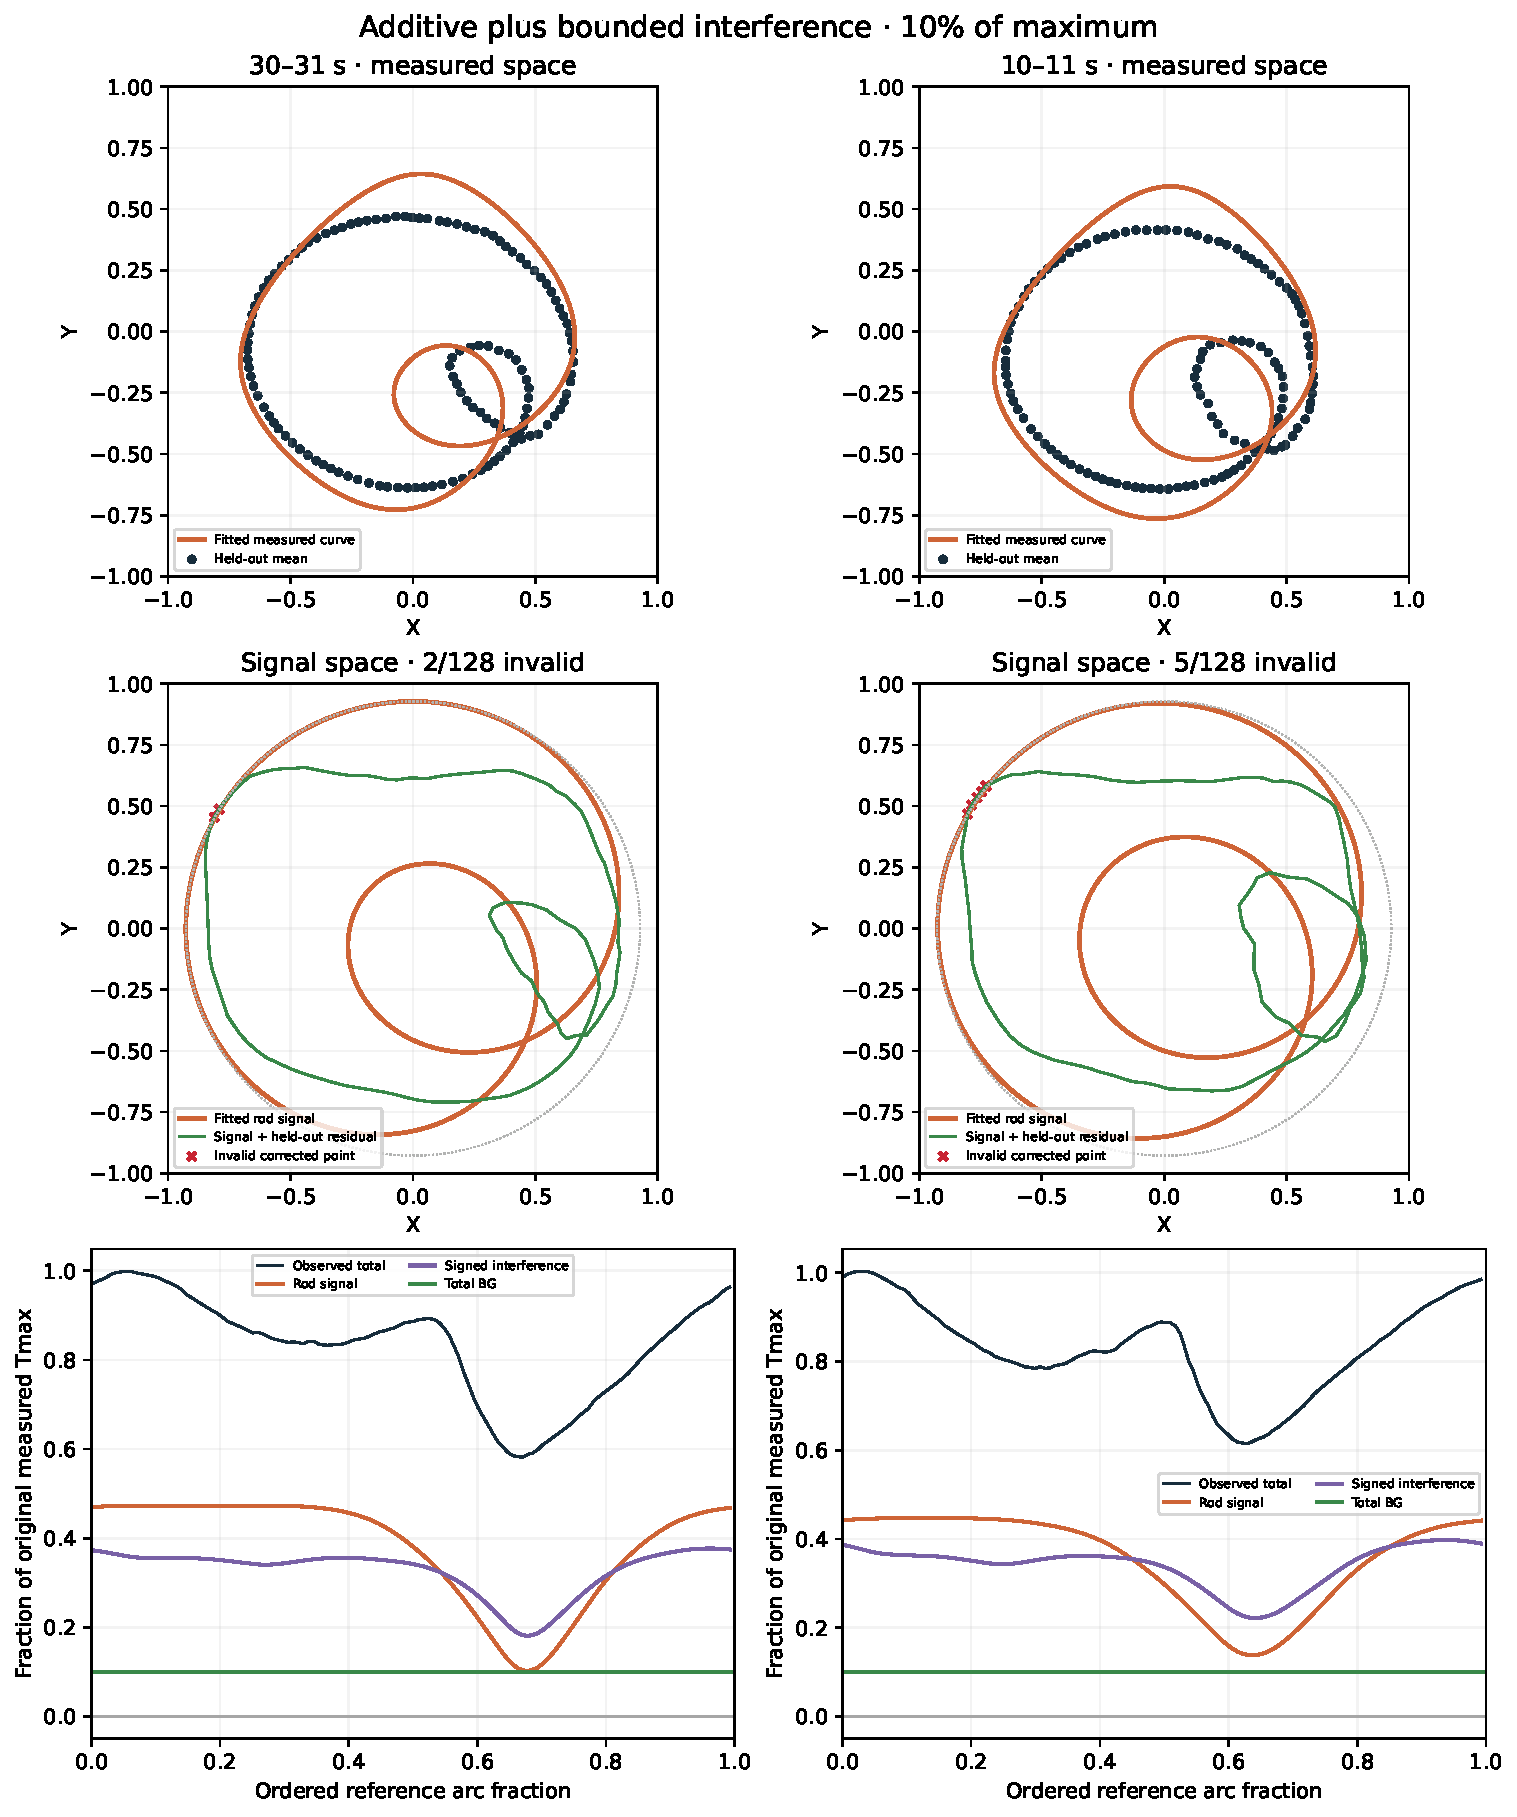
\includegraphics[width=\linewidth,height=.9\textheight,keepaspectratio]{figures/complex_10pct.pdf}
\newpage
\subsection{Representative sphere diagnostic: 10\% of maximum}
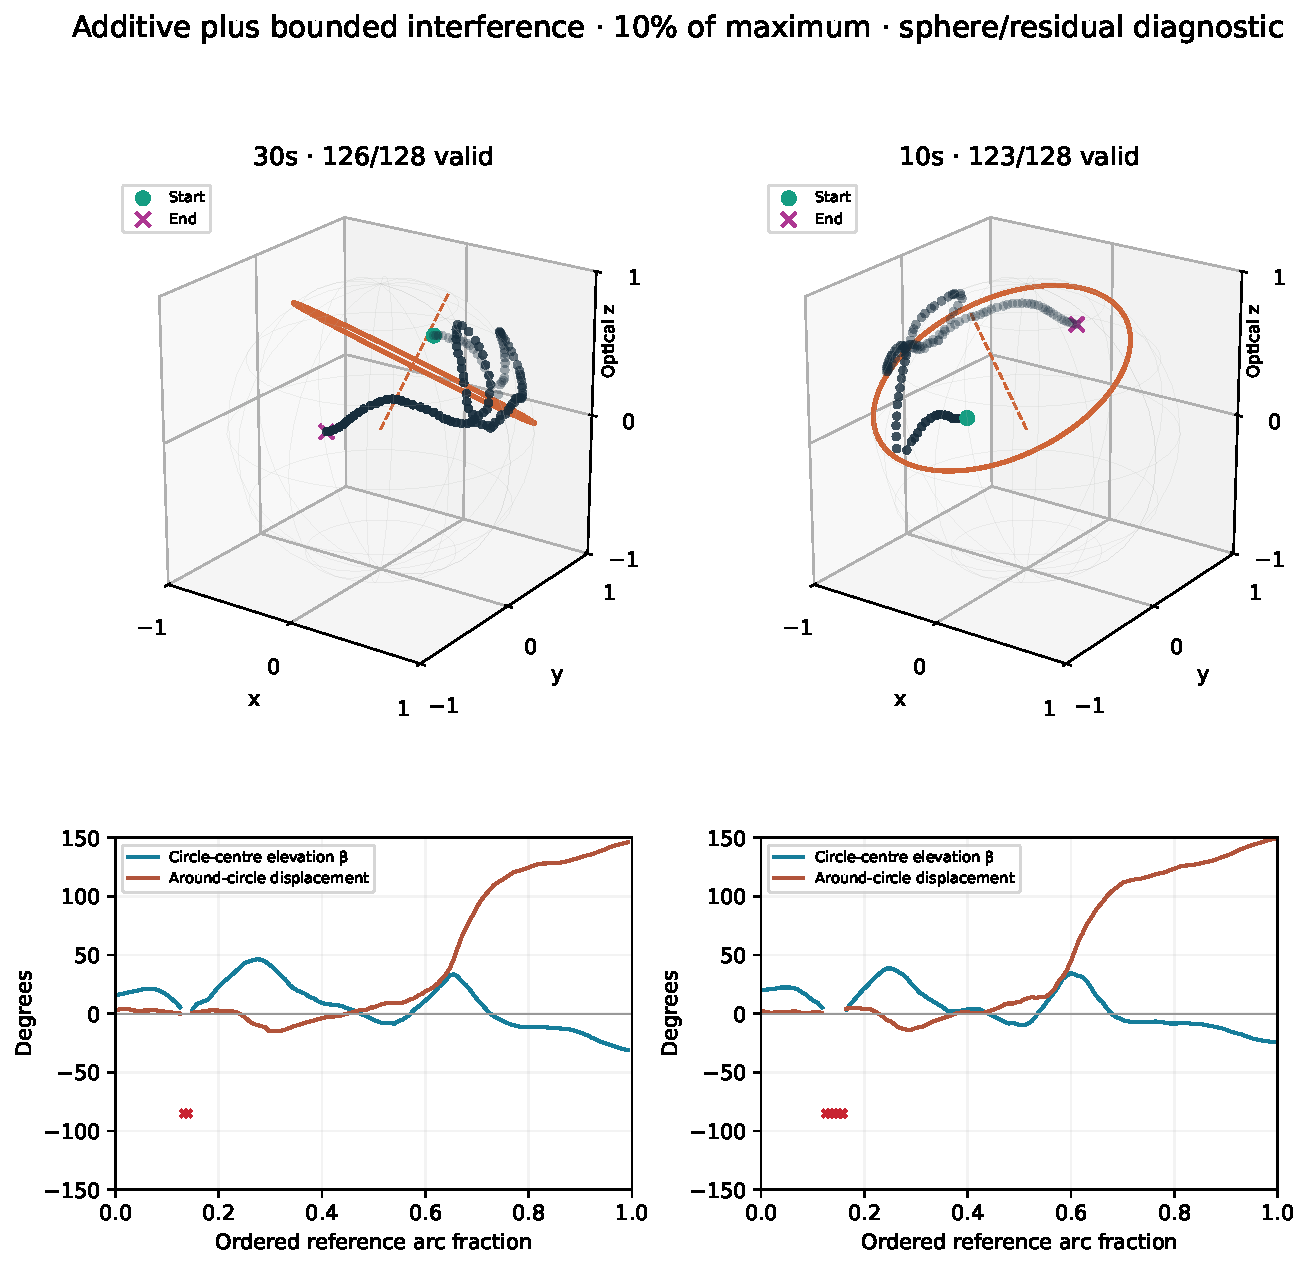
\includegraphics[width=\linewidth,height=.82\textheight,keepaspectratio]{figures/complex_sphere.pdf}
30s: 126/128 valid; matched geodesic RMS 72.60$^\circ$; closure unresolved (excluded bins); oriented endpoint mismatch 141.50$^\circ$.\par
10s: 123/128 valid; matched geodesic RMS 75.85$^\circ$; closure unresolved (excluded bins); oriented endpoint mismatch 131.32$^\circ$.\par
\newpage
\subsection{Local cone-referenced angular residual: 10\% of maximum}\label{local:complex}
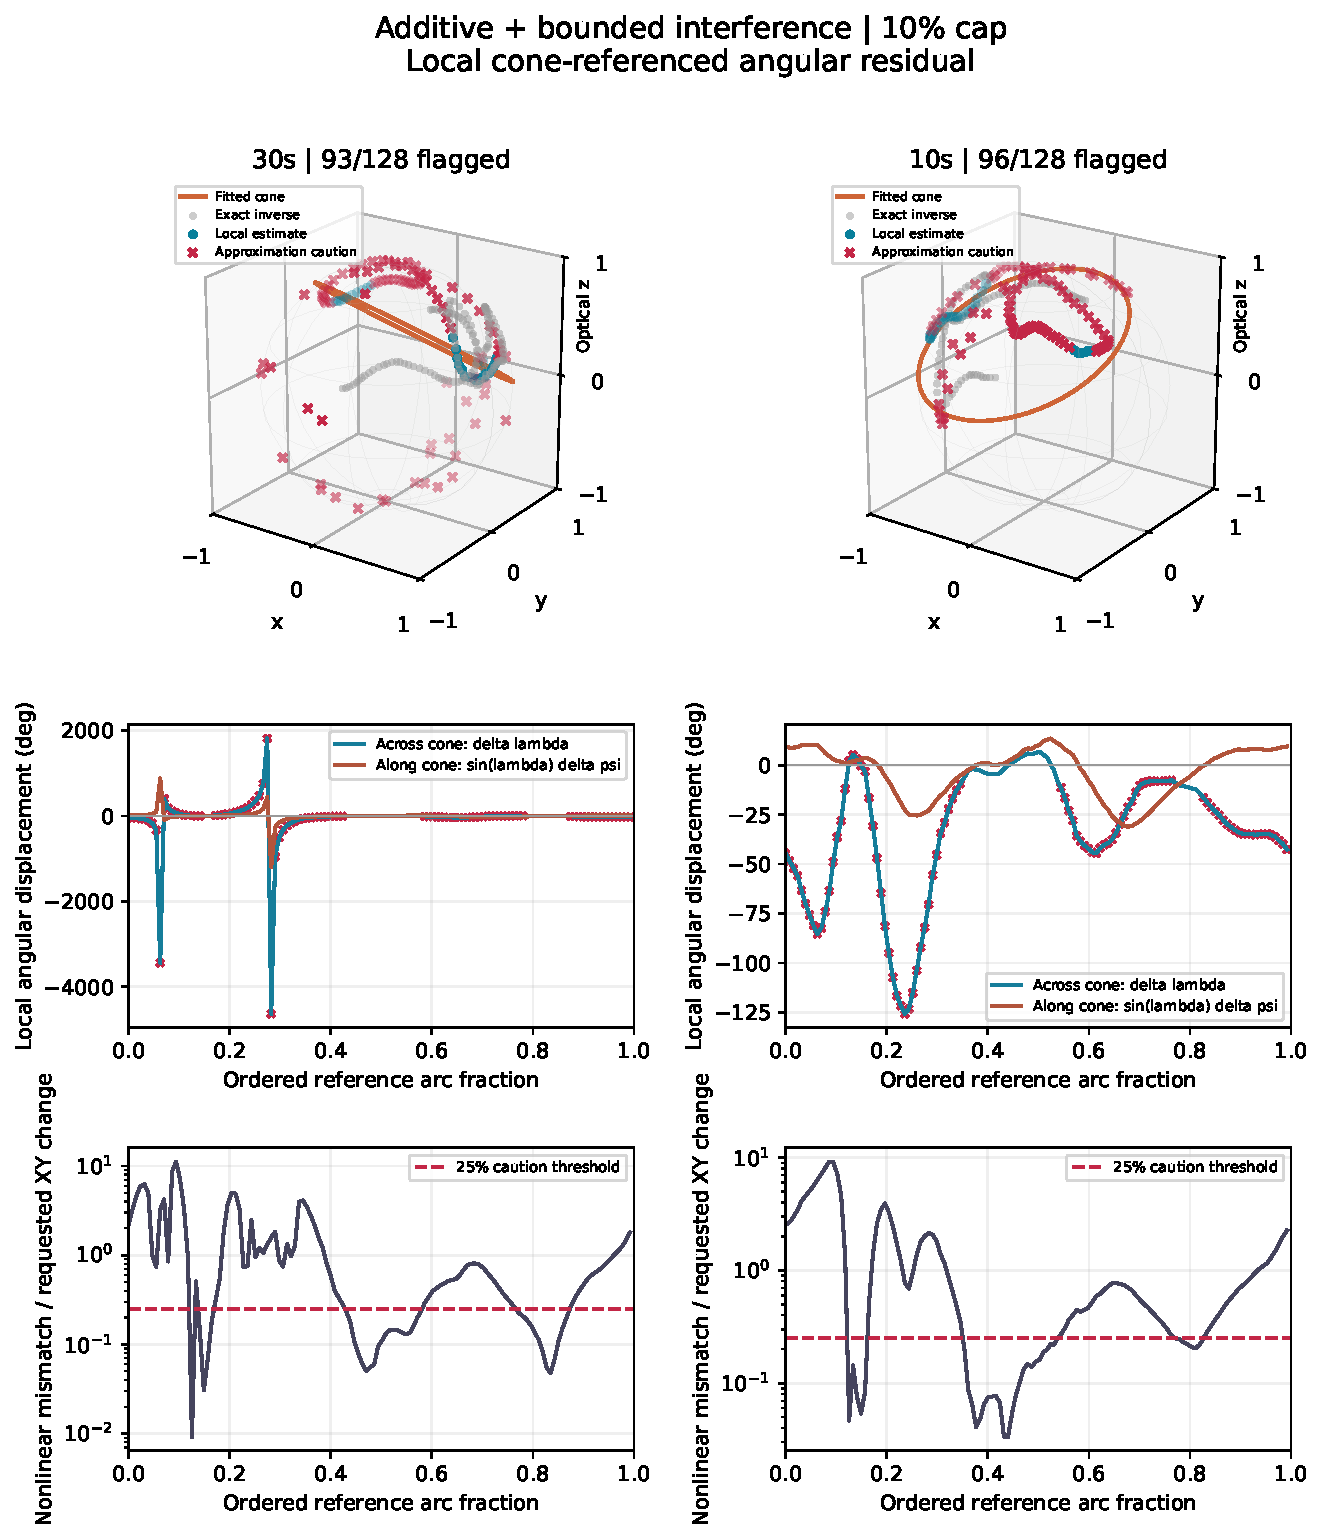
\includegraphics[width=\linewidth,height=.86\textheight,keepaspectratio]{local_residual/complex.pdf}
30s: local angular RMS 573.04$^\circ$; 93/128 caution flags; median nonlinear mismatch ratio 0.555.\par
10s: local angular RMS 46.38$^\circ$; 96/128 caution flags; median nonlinear mismatch ratio 0.539.\par
\newpage
\section{Uniform pupil field}
\[\mathbf{E}_b=b_1\mathbf{U}_x+b_2\mathbf{U}_y,\qquad I_i=S_i+I_{\mathrm{int},i}+B_i.\]
The two normalized pupil modes have uniform scalar amplitude and orthogonal transverse polarization. Fit two complex field coefficients and a noninterfering Stokes background, shared across windows. Equivalent background coordinates are total power, coherent fraction, noninterfering polarization degree/angle and three real angles specifying the normalized complex field. Seven shared background parameters plus ten local parameters. This restricts spatial overlap strongly.
\textbf{Total fitted continuous parameters across both windows: 17.} The three pre-estimated gain adjustments are additional calibration parameters, held fixed here.
\begin{longtable}{llrrrrrr}\toprule
Budget & Window & BG\% & Meas.RMS & Signal RMS & Bad(train/test) & Max $r$ & Conv.\\\midrule\endhead
uncapped & 30s & 57.1 & 0.0181 & 0.0638 & 10/6 & 0.936 & yes \\
uncapped & 10s & 56.8 & 0.0216 & 0.0881 & 7/17 & 1.035 & yes \\
5pct & 30s & 5.0 & 0.0555 & 0.0607 & 0/0 & 0.797 & yes \\
5pct & 10s & 5.0 & 0.0610 & 0.0696 & 0/0 & 0.792 & yes \\
10pct & 30s & 10.0 & 0.0432 & 0.0385 & 0/0 & 0.845 & yes \\
10pct & 10s & 10.0 & 0.0495 & 0.0459 & 0/0 & 0.834 & yes \\
20pct & 30s & 20.0 & 0.0243 & 0.0236 & 10/13 & 0.941 & yes \\
20pct & 10s & 19.9 & 0.0277 & 0.0271 & 0/0 & 0.917 & yes \\
\bottomrule\end{longtable}
\begin{longtable}{llrrrr}\toprule
Budget & Window & Signal\% range & Cross\% range & Noninterf.BG\% & Fitted folded $\theta$\\\midrule\endhead
uncapped & 30s & 5.3--126.5 & -100.0---4.7 & 11.2 & 12.5--89.9$^\circ$ \\
uncapped & 10s & 6.9--121.2 & -93.3---6.2 & 11.1 & 14.6--89.9$^\circ$ \\
5pct & 30s & 35.2--118.1 & -37.3---10.1 & 0.0 & 34.6--89.8$^\circ$ \\
5pct & 10s & 35.4--118.0 & -36.3---10.2 & 0.0 & 34.7--89.5$^\circ$ \\
10pct & 30s & 46.2--123.3 & -49.5---17.3 & 1.5 & 39.3--90.0$^\circ$ \\
10pct & 10s & 46.4--121.9 & -48.1---17.3 & 1.5 & 39.6--89.9$^\circ$ \\
20pct & 30s & 47.3--114.7 & -45.4---16.9 & 12.3 & 40.2--77.0$^\circ$ \\
20pct & 10s & 53.6--112.8 & -44.1---17.9 & 12.3 & 43.0--74.4$^\circ$ \\
\bottomrule\end{longtable}
\textbf{Per-channel constant background, percent of measured maximum:}
\begin{longtable}{llrrrr}\toprule
Budget & Window & $B_0$ & $B_{90}$ & $B_{45}$ & $B_{135}$\\\midrule\endhead
uncapped & 30s & 17.35 & 11.20 & 10.63 & 17.93\\
uncapped & 10s & 17.27 & 11.15 & 10.58 & 17.84\\
5pct & 30s & 1.41 & 1.09 & 1.60 & 0.90\\
5pct & 10s & 1.40 & 1.08 & 1.59 & 0.90\\
10pct & 30s & 2.78 & 2.22 & 2.67 & 2.33\\
10pct & 10s & 2.77 & 2.21 & 2.66 & 2.32\\
20pct & 30s & 6.69 & 3.31 & 3.02 & 6.98\\
20pct & 10s & 6.66 & 3.29 & 3.01 & 6.95\\
\bottomrule\end{longtable}
\newpage
\subsection{No BG-power cap}\label{case:uniform:uncapped}
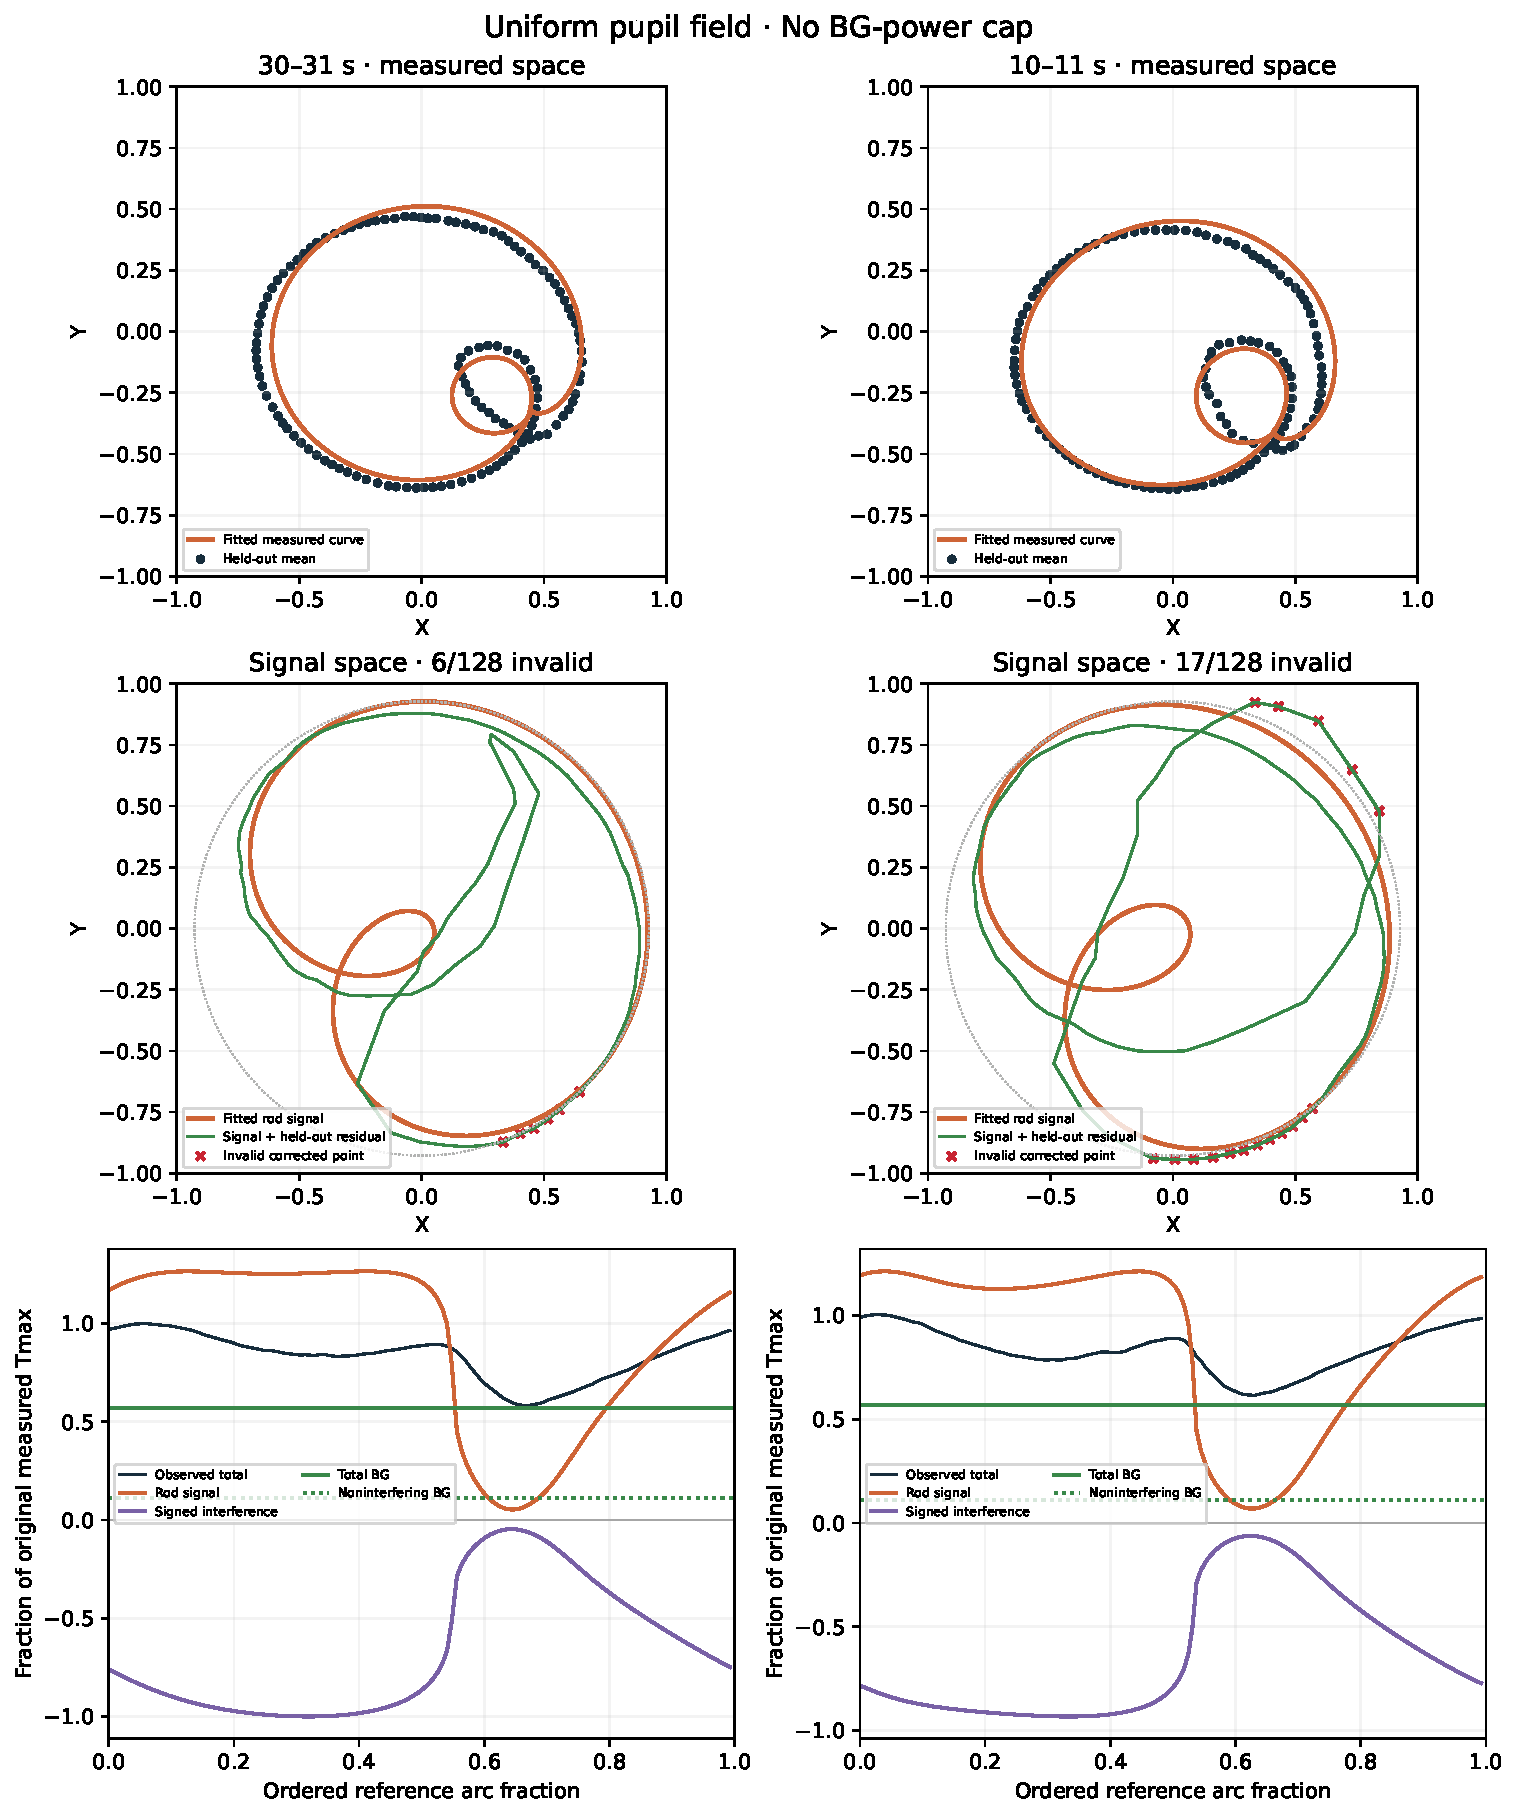
\includegraphics[width=\linewidth,height=.9\textheight,keepaspectratio]{figures/uniform_uncapped.pdf}
\newpage
\subsection{5\% of maximum}\label{case:uniform:5pct}
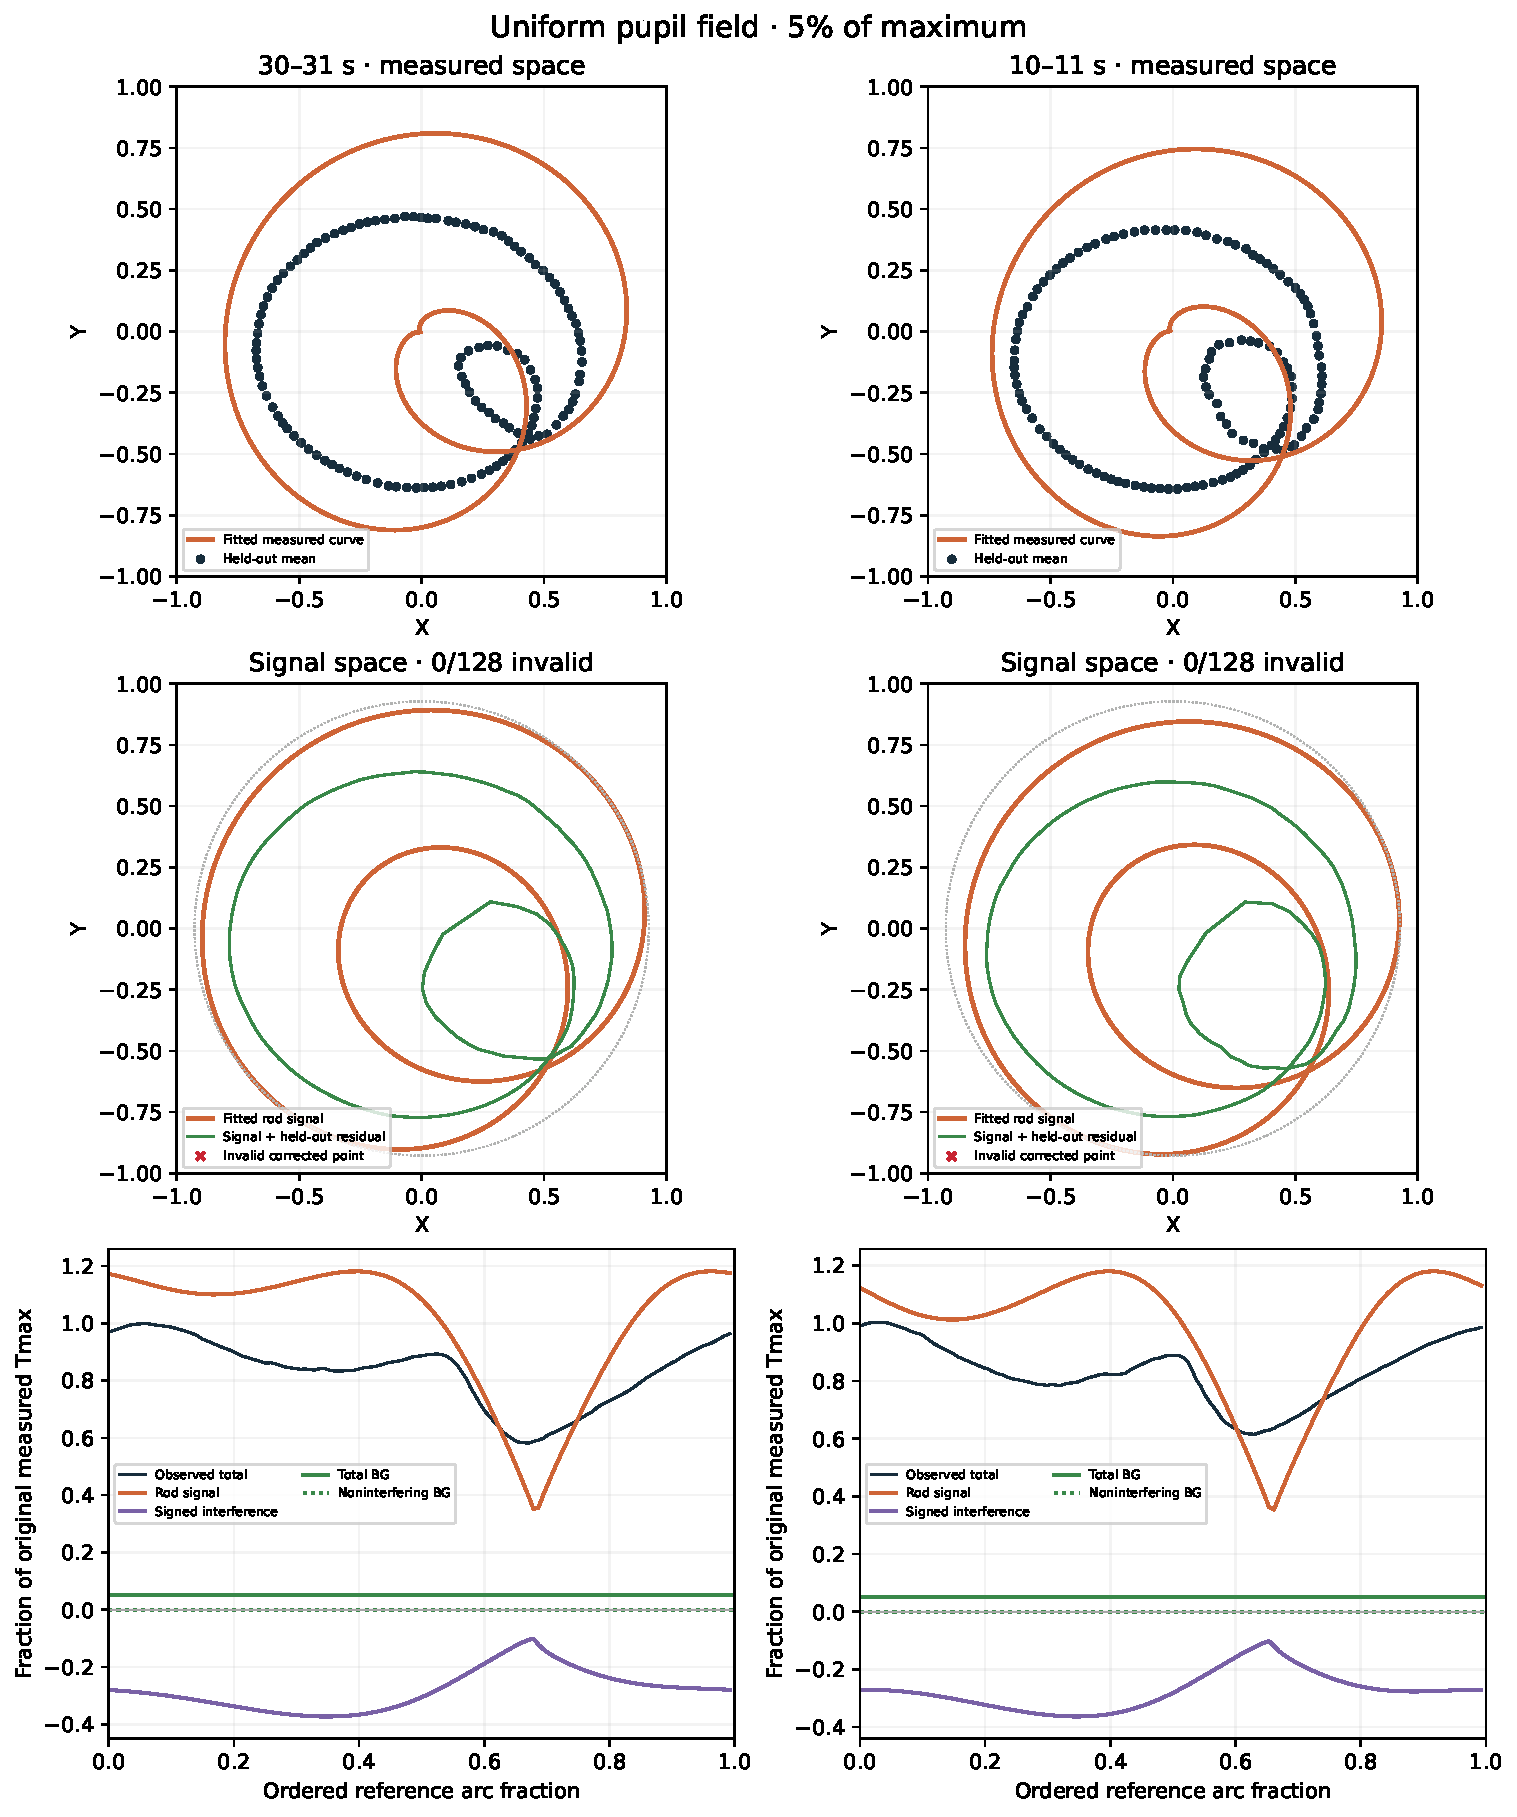
\includegraphics[width=\linewidth,height=.9\textheight,keepaspectratio]{figures/uniform_5pct.pdf}
\newpage
\subsection{10\% of maximum}\label{case:uniform:10pct}
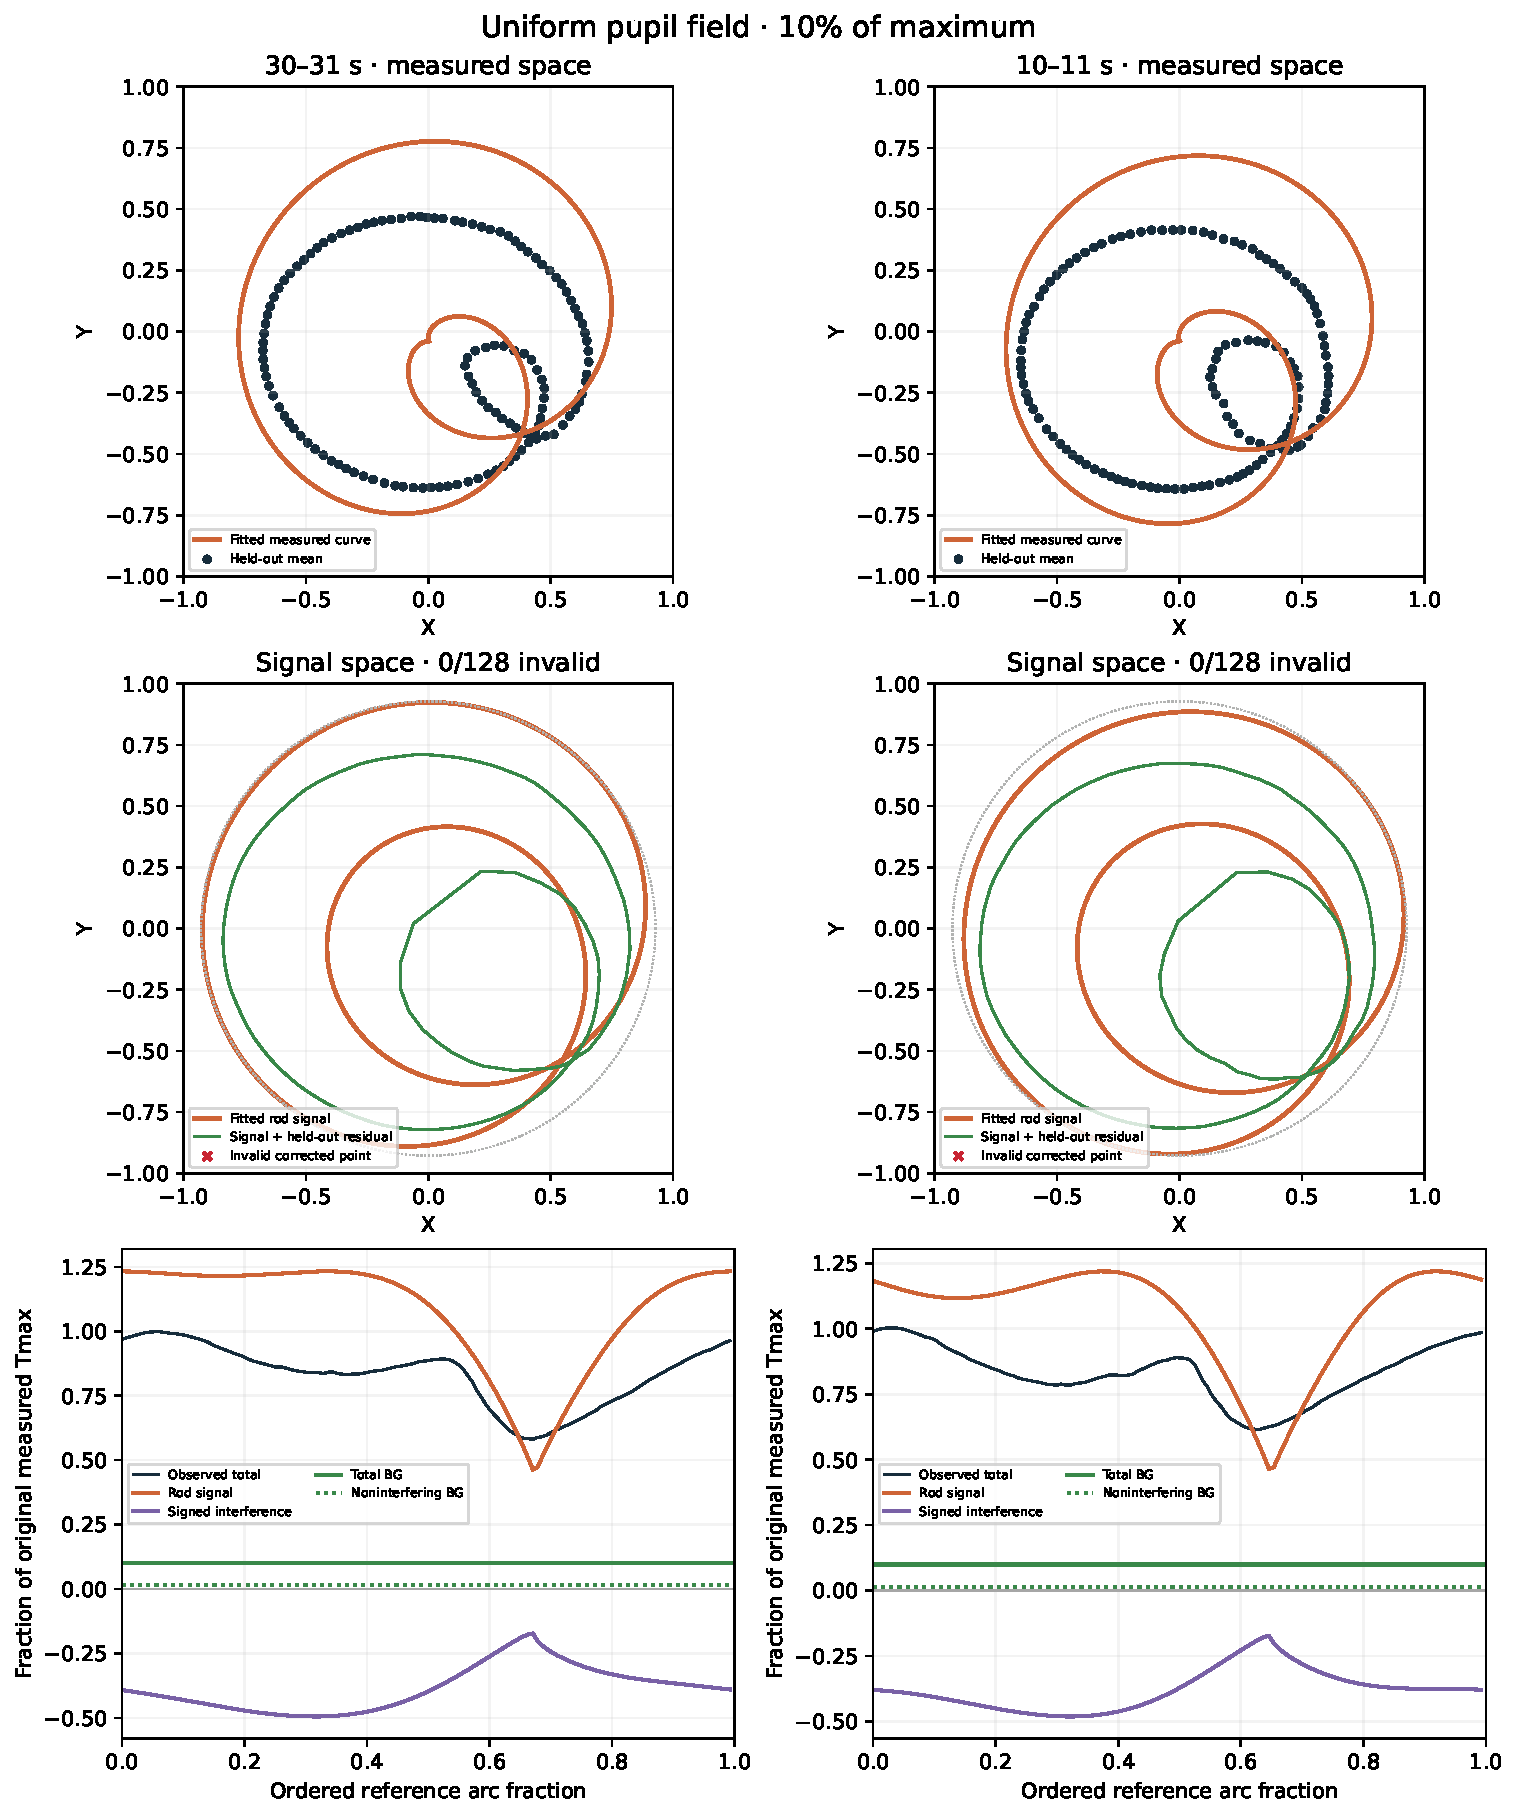
\includegraphics[width=\linewidth,height=.9\textheight,keepaspectratio]{figures/uniform_10pct.pdf}
\newpage
\subsection{20\% of maximum}\label{case:uniform:20pct}
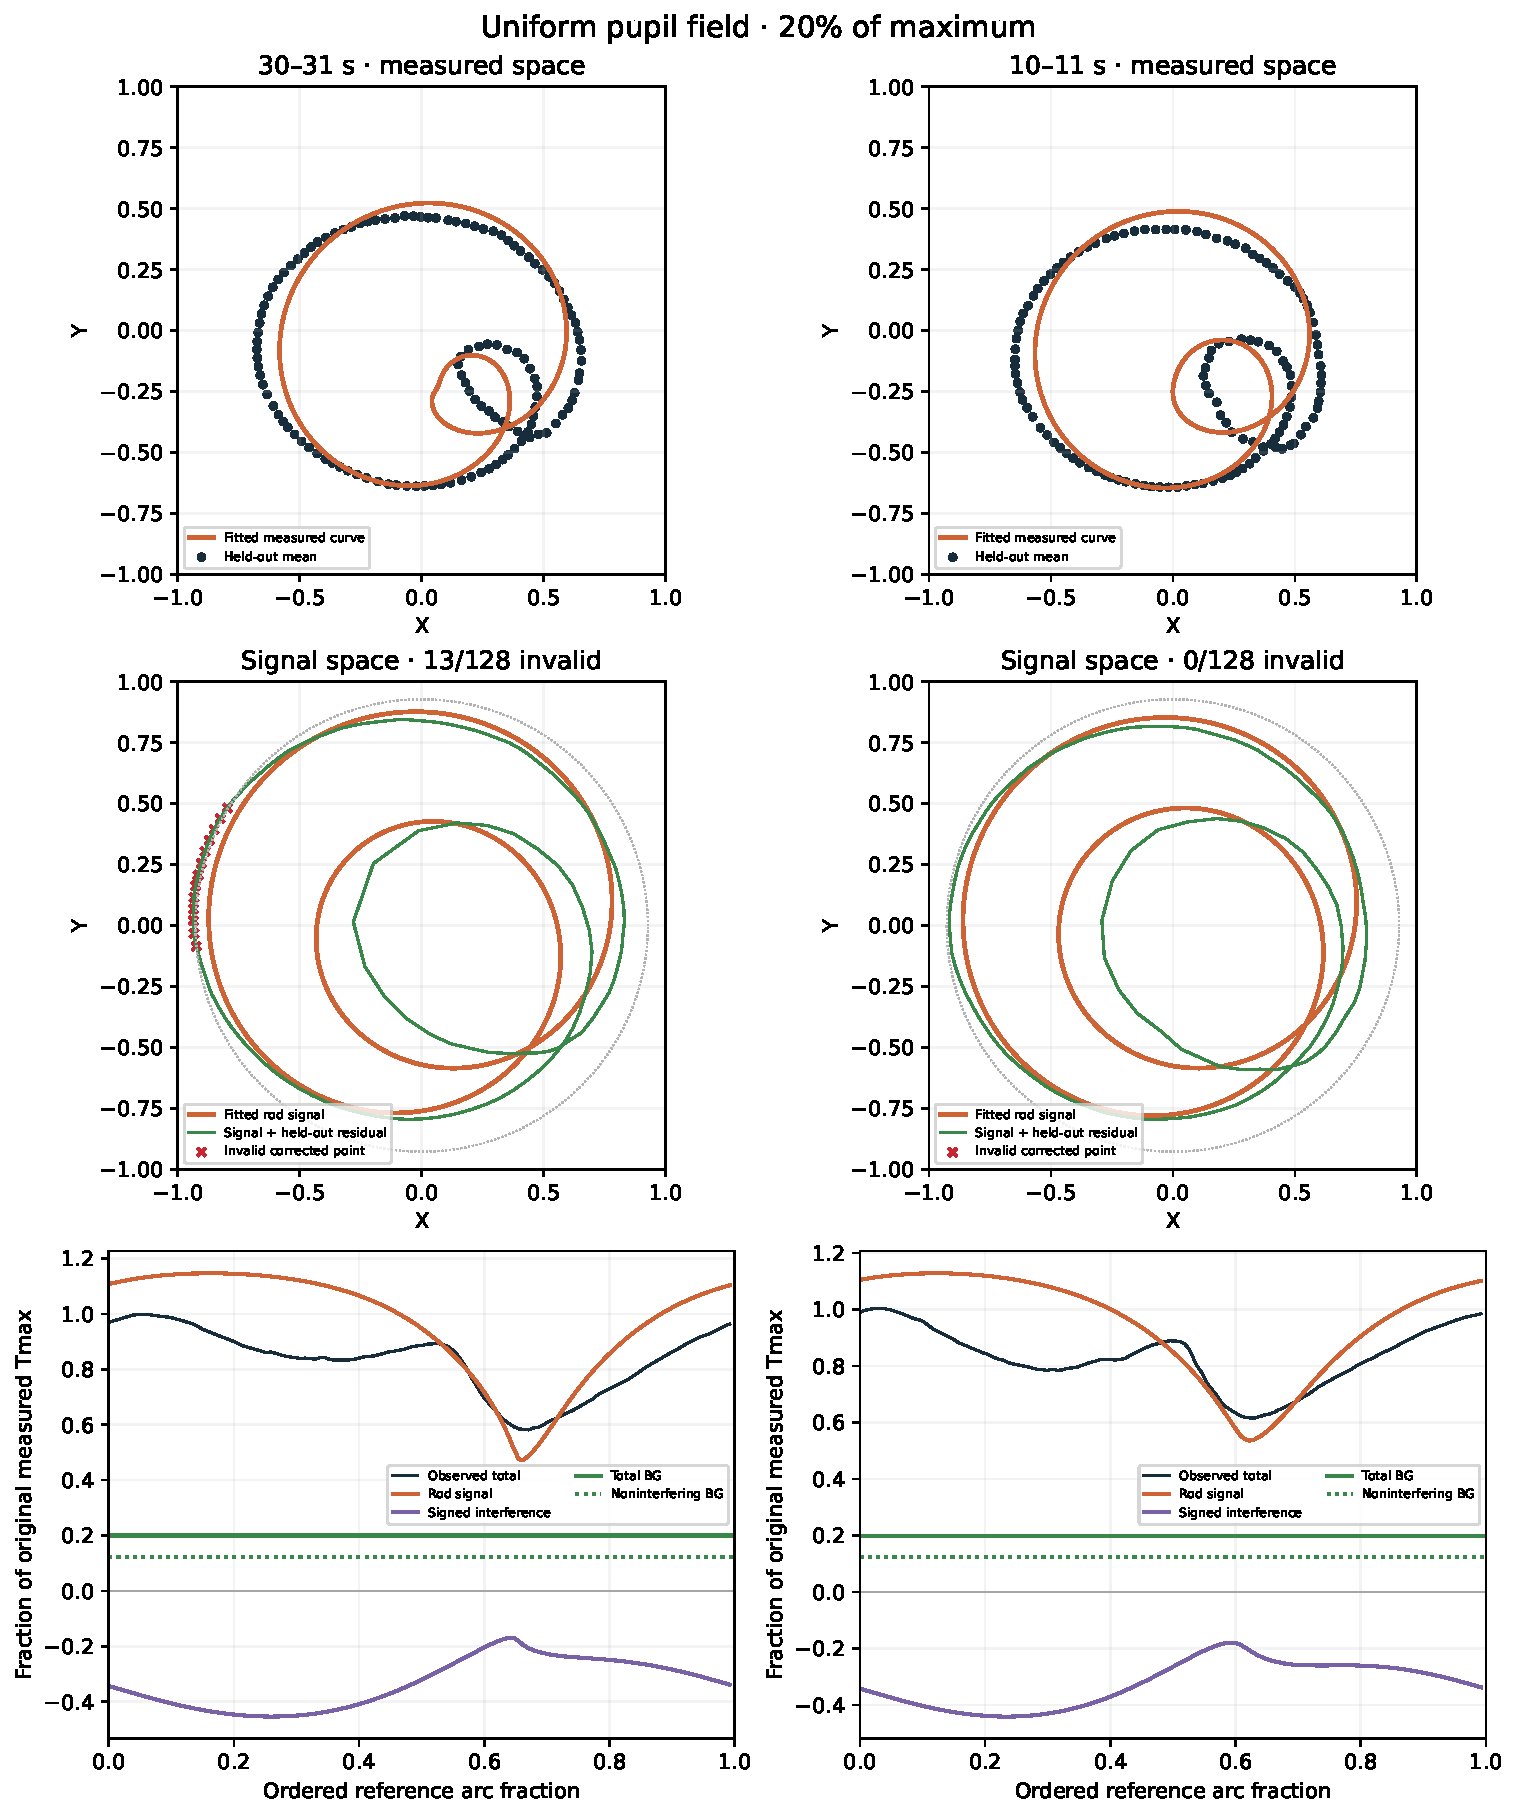
\includegraphics[width=\linewidth,height=.9\textheight,keepaspectratio]{figures/uniform_20pct.pdf}
\newpage
\subsection{Representative sphere diagnostic: 10\% of maximum}
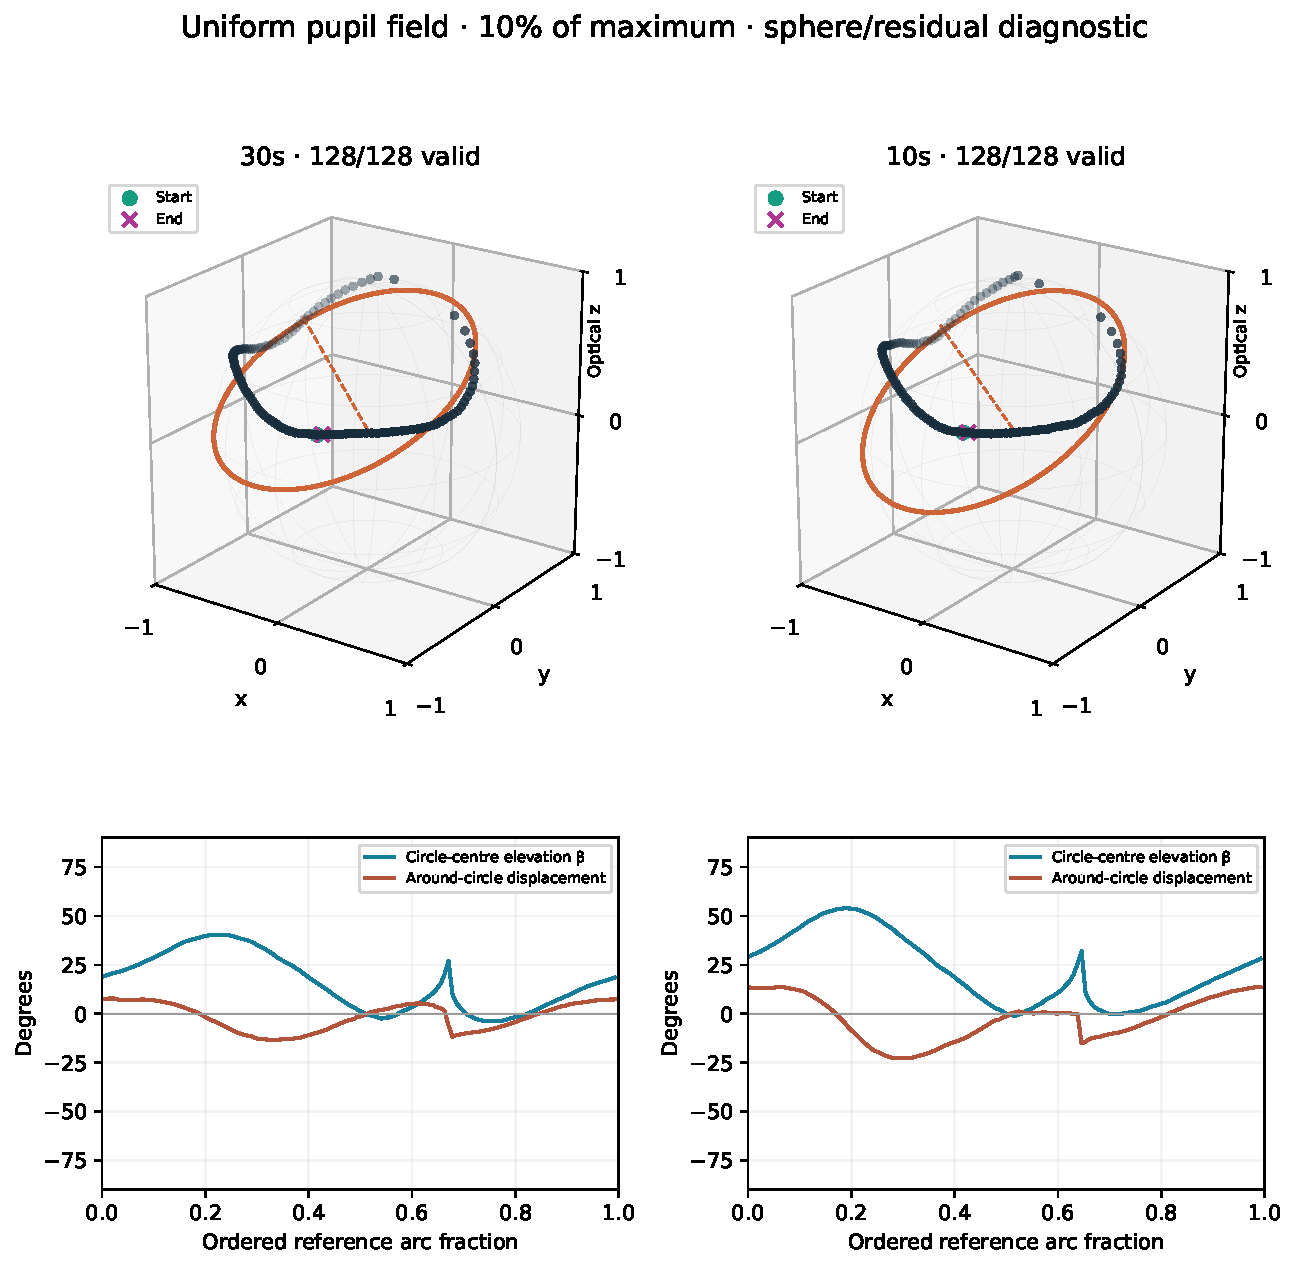
\includegraphics[width=\linewidth,height=.82\textheight,keepaspectratio]{figures/uniform_sphere.pdf}
30s: 128/128 valid; matched geodesic RMS 20.17$^\circ$; oriented closure mismatch 0.00$^\circ$.\par
10s: 128/128 valid; matched geodesic RMS 27.23$^\circ$; oriented closure mismatch 0.00$^\circ$.\par
\newpage
\subsection{Local cone-referenced angular residual: 10\% of maximum}\label{local:uniform}
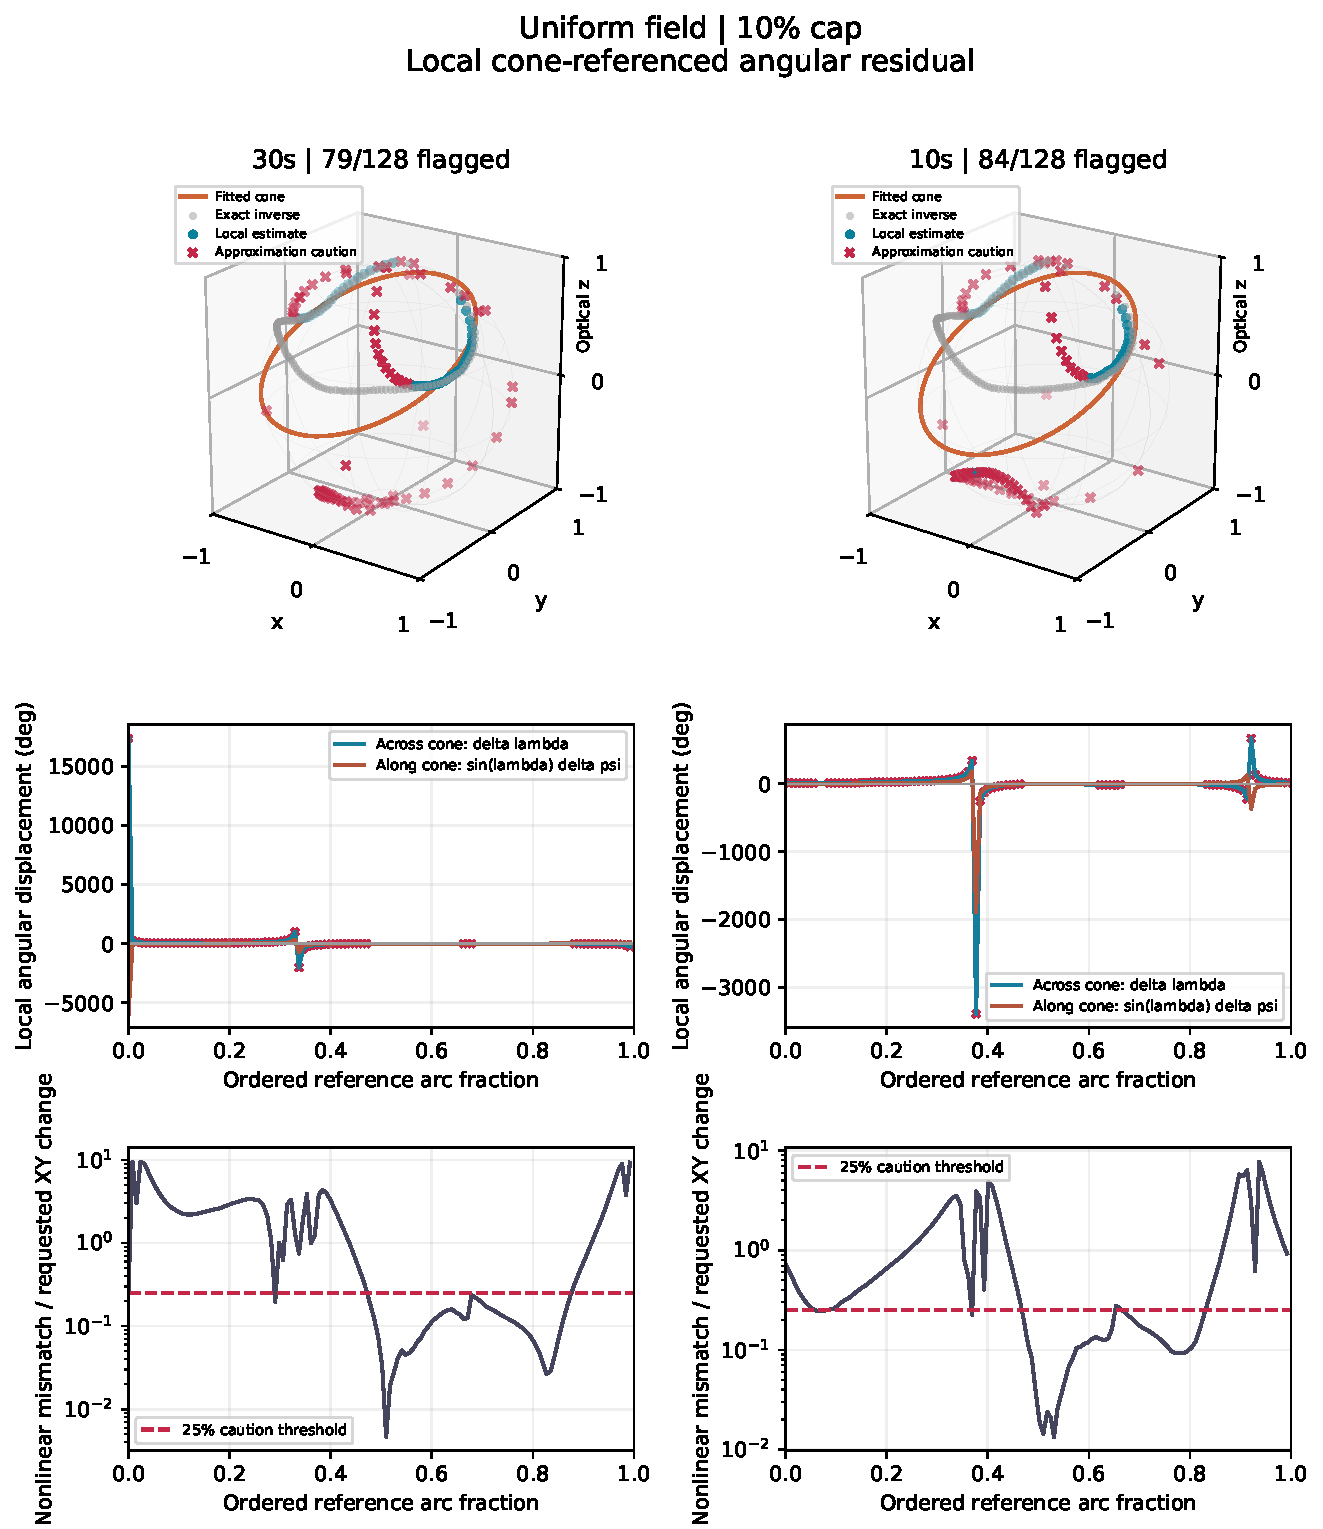
\includegraphics[width=\linewidth,height=.86\textheight,keepaspectratio]{local_residual/uniform.pdf}
30s: local angular RMS 1640.48$^\circ$; 79/128 caution flags; median nonlinear mismatch ratio 0.832.\par
10s: local angular RMS 356.01$^\circ$; 84/128 caution flags; median nonlinear mismatch ratio 0.373.\par
\newpage
\section{Three-mode field}
\[\mathbf{E}_b=b_1\mathbf{U}_x+b_2\mathbf{U}_y+b_3\mathbf{U}_{d_z},\qquad I_i=S_i+I_{\mathrm{int},i}+B_i.\]
Add a dipole-derived longitudinal-orientation pupil field to the two uniform modes, orthonormalized under the detector integral. Three complex coefficients plus noninterfering Stokes background: nine shared background parameters and ten local parameters. This is the earlier radial/dipole-overlap family expressed as a common stationary field.
\textbf{Total fitted continuous parameters across both windows: 19.} The three pre-estimated gain adjustments are additional calibration parameters, held fixed here.
\begin{longtable}{llrrrrrr}\toprule
Budget & Window & BG\% & Meas.RMS & Signal RMS & Bad(train/test) & Max $r$ & Conv.\\\midrule\endhead
uncapped & 30s & 55.0 & 0.0074 & 0.0302 & 15/18 & 1.051 & yes \\
uncapped & 10s & 54.8 & 0.0127 & 0.0390 & 10/22 & 1.087 & yes \\
5pct & 30s & 5.0 & 0.0475 & 0.0598 & 0/0 & 0.810 & yes \\
5pct & 10s & 5.0 & 0.0532 & 0.0693 & 0/0 & 0.809 & yes \\
10pct & 30s & 10.0 & 0.0344 & 0.0357 & 0/0 & 0.868 & yes \\
10pct & 10s & 10.0 & 0.0401 & 0.0441 & 0/0 & 0.877 & yes \\
20pct & 30s & 20.0 & 0.0164 & 0.0248 & 0/0 & 0.754 & yes \\
20pct & 10s & 19.9 & 0.0187 & 0.0276 & 0/0 & 0.713 & yes \\
30pct & 30s & 30.0 & 0.0140 & 0.0266 & 0/0 & 0.709 & yes \\
30pct & 10s & 29.9 & 0.0163 & 0.0296 & 0/0 & 0.653 & yes \\
40pct & 30s & 40.0 & 0.0133 & 0.0343 & 0/0 & 0.697 & yes \\
40pct & 10s & 39.8 & 0.0156 & 0.0375 & 0/0 & 0.643 & yes \\
50pct & 30s & 50.0 & 0.0075 & 0.0156 & 6/15 & 0.942 & yes \\
50pct & 10s & 49.8 & 0.0140 & 0.0364 & 6/8 & 0.936 & yes \\
\bottomrule\end{longtable}
\begin{longtable}{llrrrr}\toprule
Budget & Window & Signal\% range & Cross\% range & Noninterf.BG\% & Fitted folded $\theta$\\\midrule\endhead
uncapped & 30s & 4.9--126.5 & -97.1--4.2 & 8.6 & 12.1--89.8$^\circ$ \\
uncapped & 10s & 7.2--118.5 & -90.5--3.6 & 8.6 & 15.1--89.9$^\circ$ \\
5pct & 30s & 26.3--106.7 & -26.0--5.7 & 0.0 & 31.2--89.8$^\circ$ \\
5pct & 10s & 28.1--104.9 & -24.4--5.4 & 0.0 & 32.6--89.8$^\circ$ \\
10pct & 30s & 30.3--106.6 & -33.2--10.3 & 0.0 & 33.7--89.8$^\circ$ \\
10pct & 10s & 31.7--103.7 & -30.8--9.8 & 0.0 & 35.0--89.6$^\circ$ \\
20pct & 30s & 24.3--96.5 & -26.9--19.9 & 13.1 & 26.1--58.3$^\circ$ \\
20pct & 10s & 29.9--92.6 & -26.9--20.9 & 13.0 & 29.1--56.4$^\circ$ \\
30pct & 30s & 17.2--90.6 & -32.4--19.0 & 12.2 & 21.9--56.3$^\circ$ \\
30pct & 10s & 22.1--86.6 & -32.1--20.1 & 12.2 & 24.7--53.7$^\circ$ \\
40pct & 30s & 11.4--76.1 & -28.8--16.2 & 11.2 & 19.5--56.2$^\circ$ \\
40pct & 10s & 15.8--72.4 & -28.2--17.2 & 11.2 & 22.6--53.1$^\circ$ \\
50pct & 30s & 5.5--119.1 & -84.9--6.8 & 8.9 & 13.2--89.9$^\circ$ \\
50pct & 10s & 8.7--110.8 & -78.7--6.4 & 8.8 & 17.1--89.7$^\circ$ \\
\bottomrule\end{longtable}
\textbf{Per-channel constant background, percent of measured maximum:}
\begin{longtable}{llrrrr}\toprule
Budget & Window & $B_0$ & $B_{90}$ & $B_{45}$ & $B_{135}$\\\midrule\endhead
uncapped & 30s & 17.14 & 10.37 & 10.38 & 17.13\\
uncapped & 10s & 17.06 & 10.32 & 10.33 & 17.05\\
5pct & 30s & 1.29 & 1.21 & 1.61 & 0.89\\
5pct & 10s & 1.28 & 1.21 & 1.61 & 0.88\\
10pct & 30s & 2.47 & 2.53 & 3.11 & 1.89\\
10pct & 10s & 2.46 & 2.51 & 3.10 & 1.88\\
20pct & 30s & 8.35 & 1.65 & 2.61 & 7.39\\
20pct & 10s & 8.31 & 1.64 & 2.59 & 7.36\\
30pct & 30s & 11.92 & 3.08 & 4.17 & 10.83\\
30pct & 10s & 11.87 & 3.06 & 4.15 & 10.78\\
40pct & 30s & 14.72 & 5.28 & 6.23 & 13.77\\
40pct & 10s & 14.65 & 5.25 & 6.21 & 13.70\\
50pct & 30s & 16.04 & 8.96 & 9.48 & 15.52\\
50pct & 10s & 15.97 & 8.92 & 9.44 & 15.45\\
\bottomrule\end{longtable}
\newpage
\subsection{No BG-power cap}\label{case:three:uncapped}
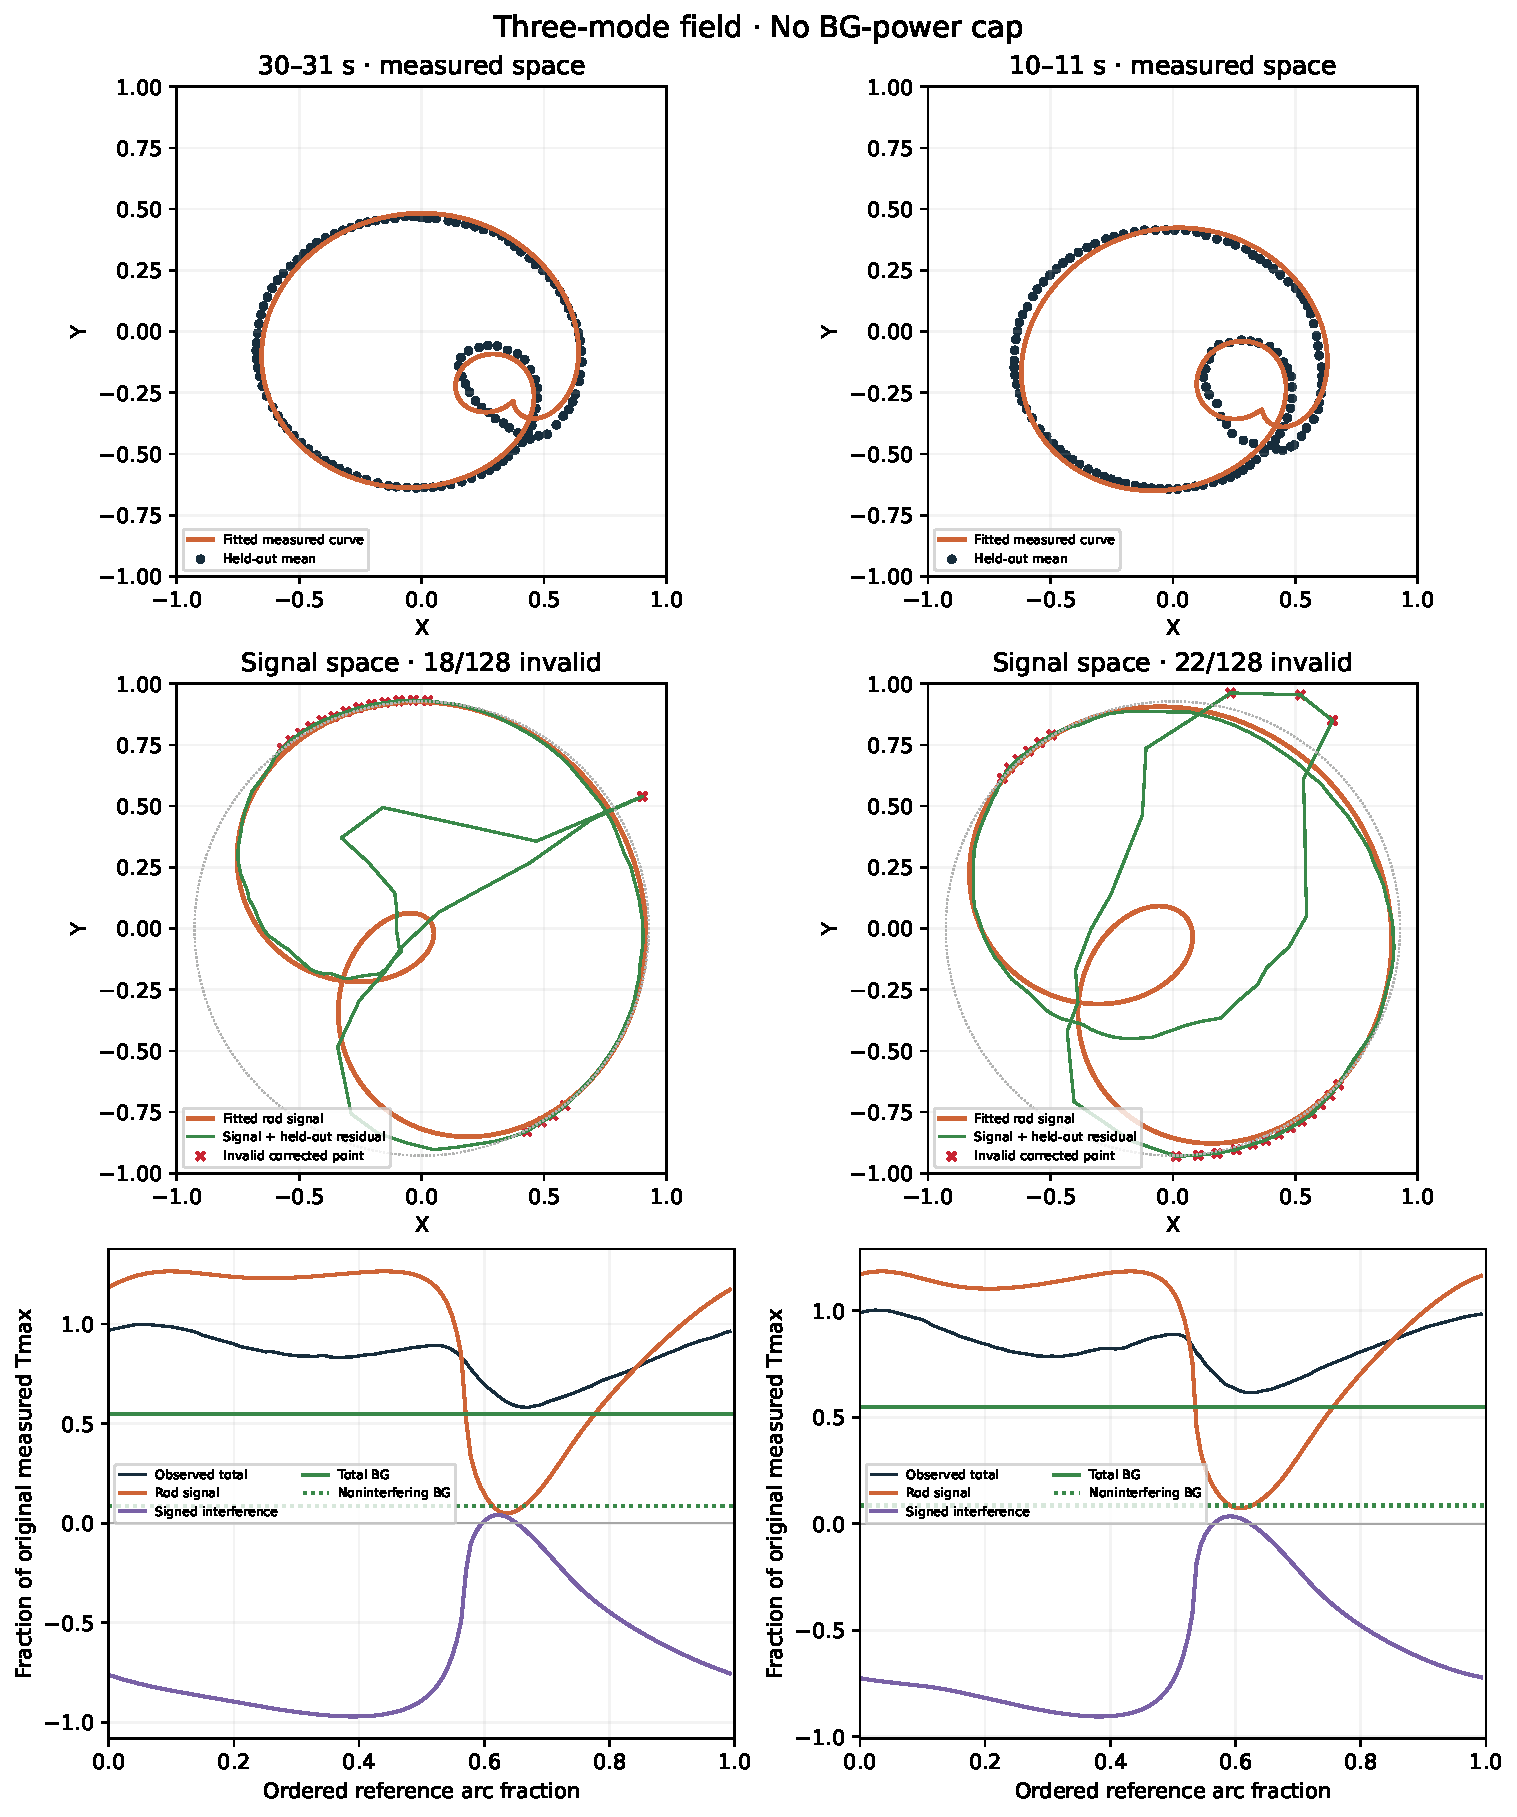
\includegraphics[width=\linewidth,height=.9\textheight,keepaspectratio]{figures/three_uncapped.pdf}
\newpage
\subsection{5\% of maximum}\label{case:three:5pct}
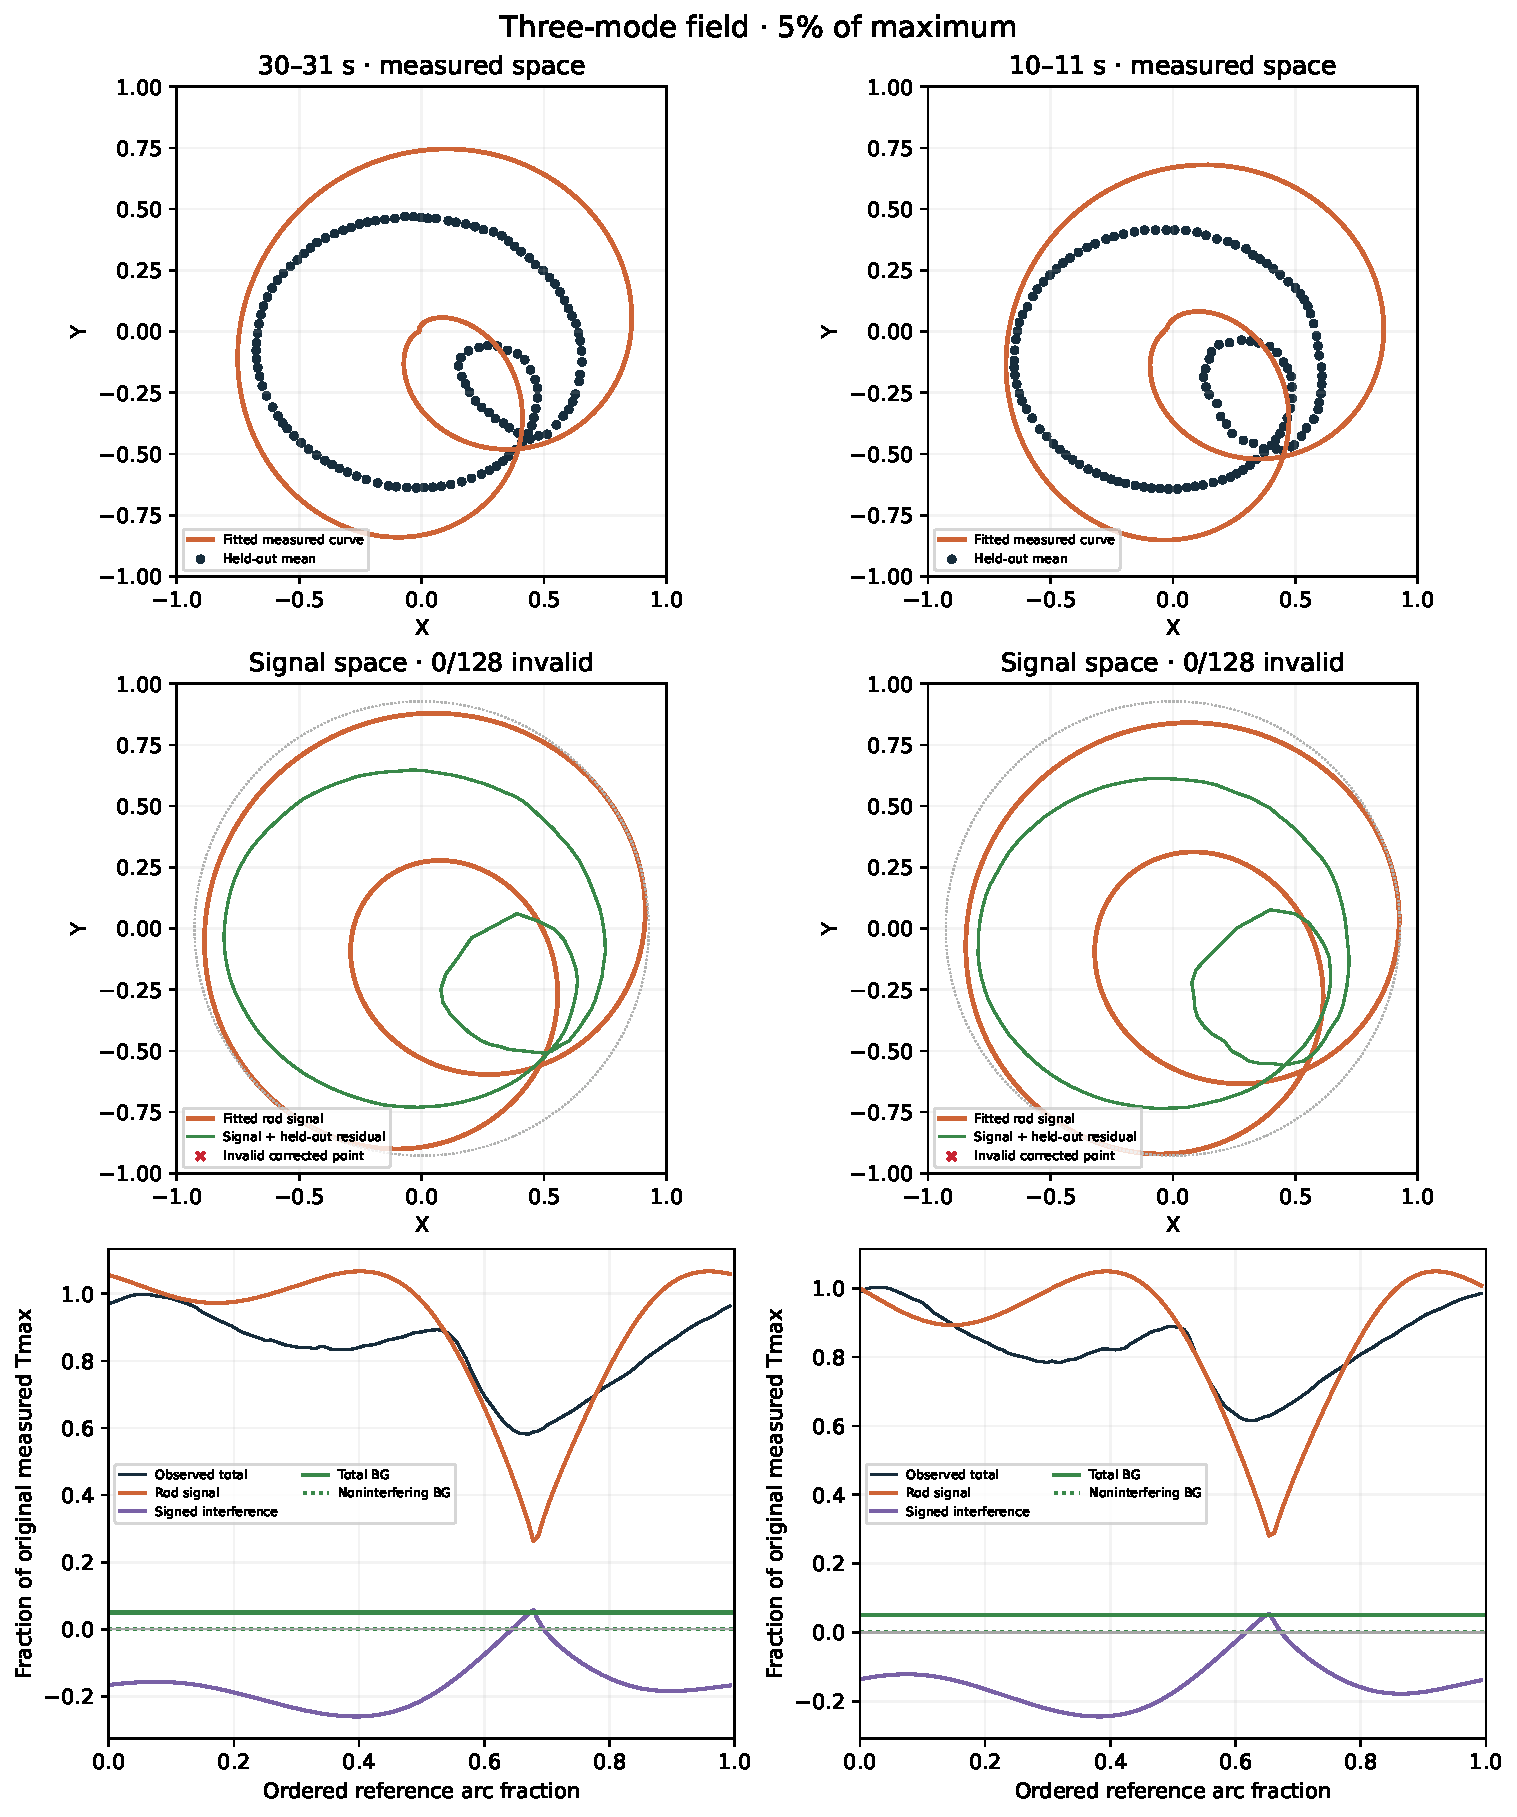
\includegraphics[width=\linewidth,height=.9\textheight,keepaspectratio]{figures/three_5pct.pdf}
\newpage
\subsection{10\% of maximum}\label{case:three:10pct}
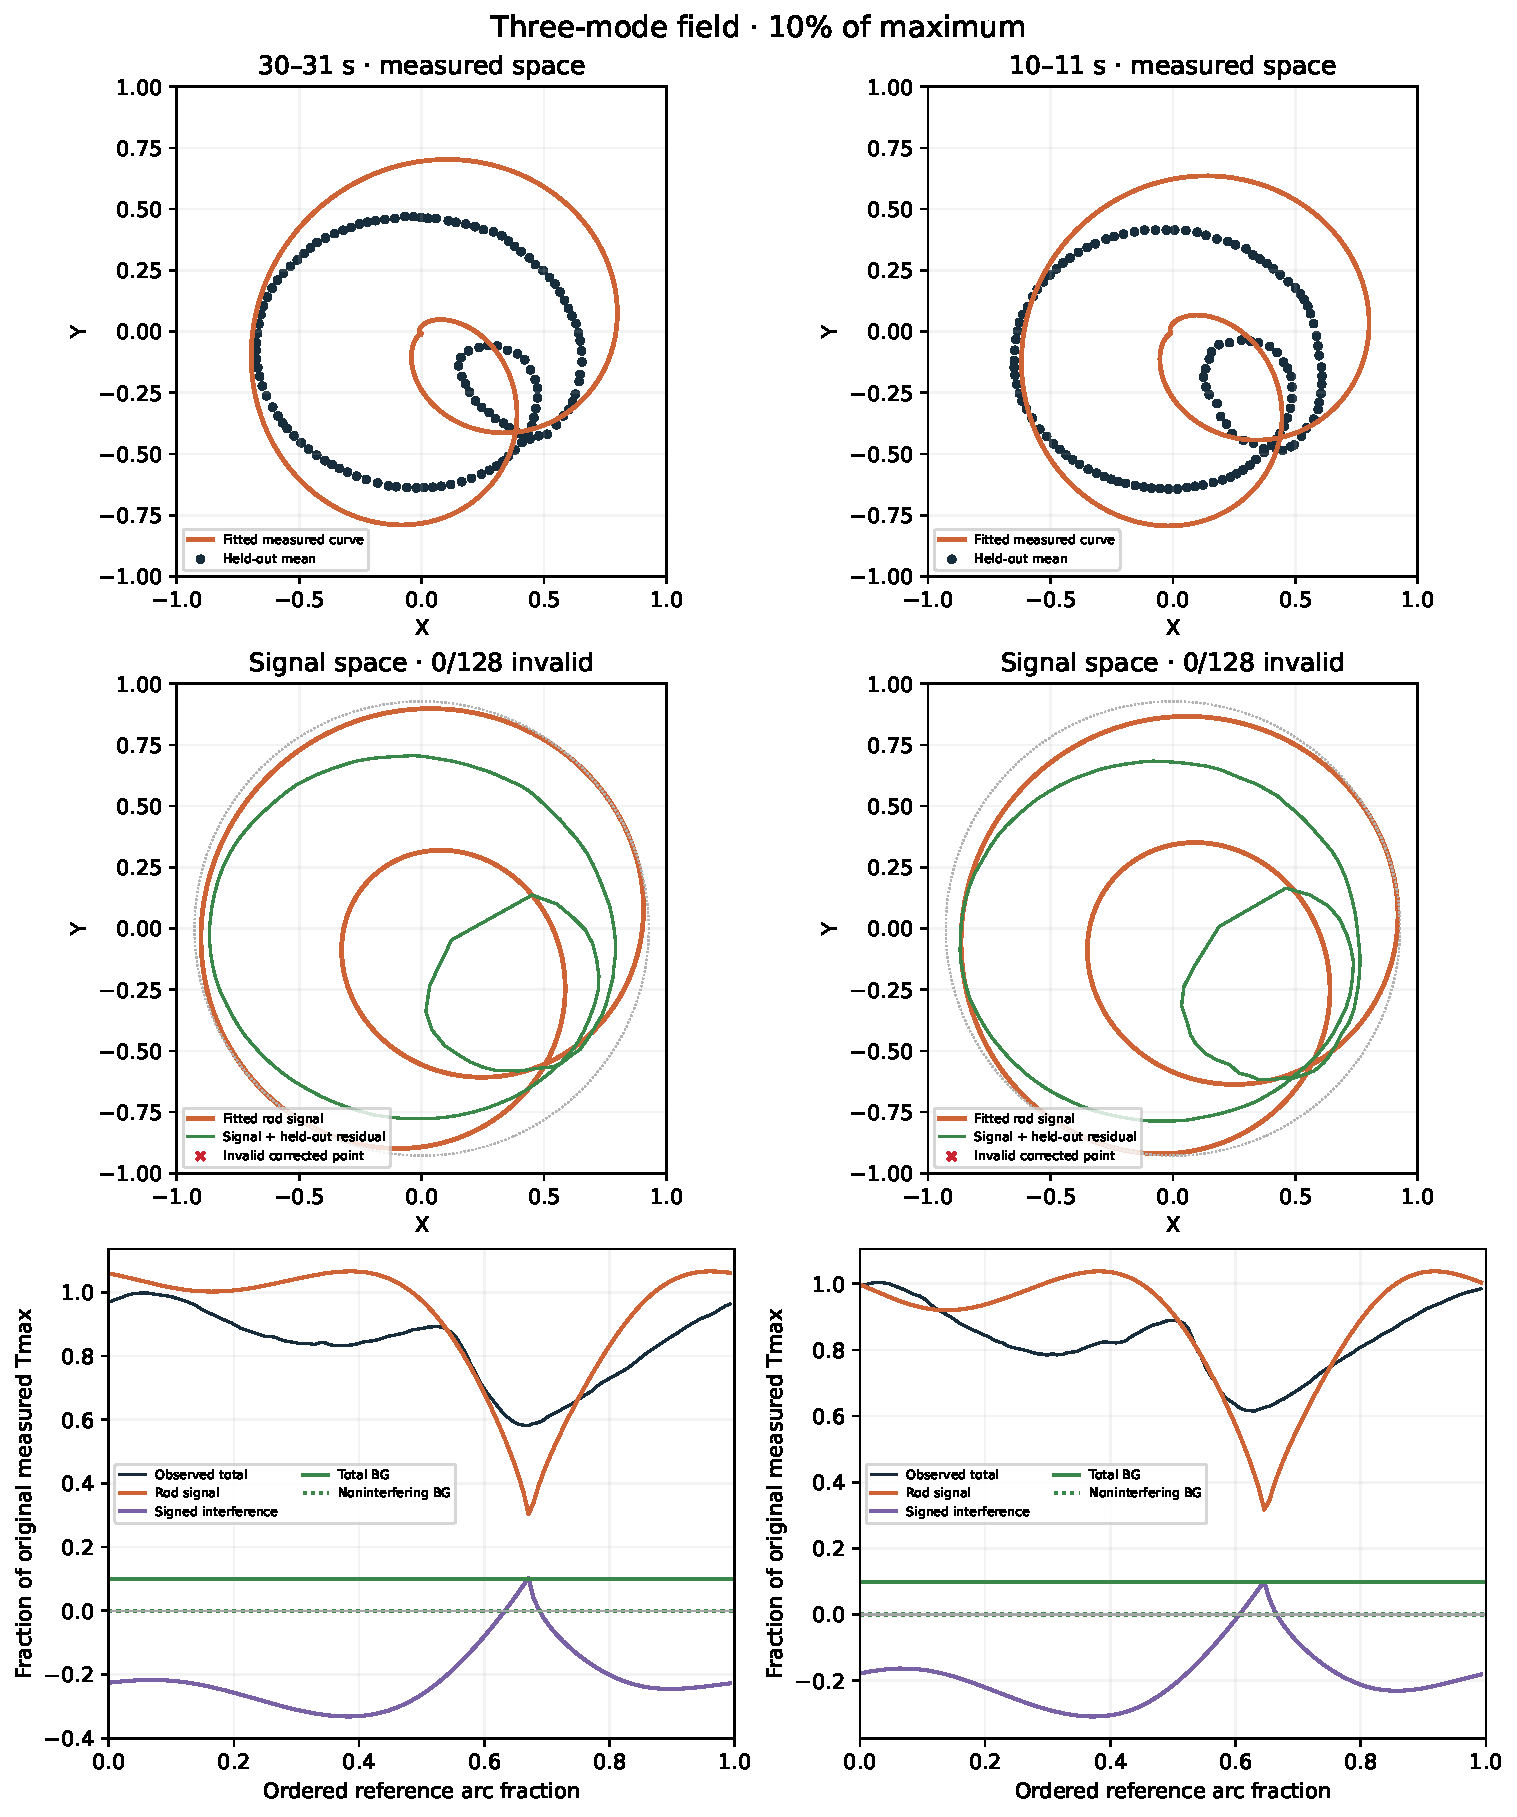
\includegraphics[width=\linewidth,height=.9\textheight,keepaspectratio]{figures/three_10pct.pdf}
\newpage
\subsection{20\% of maximum}\label{case:three:20pct}
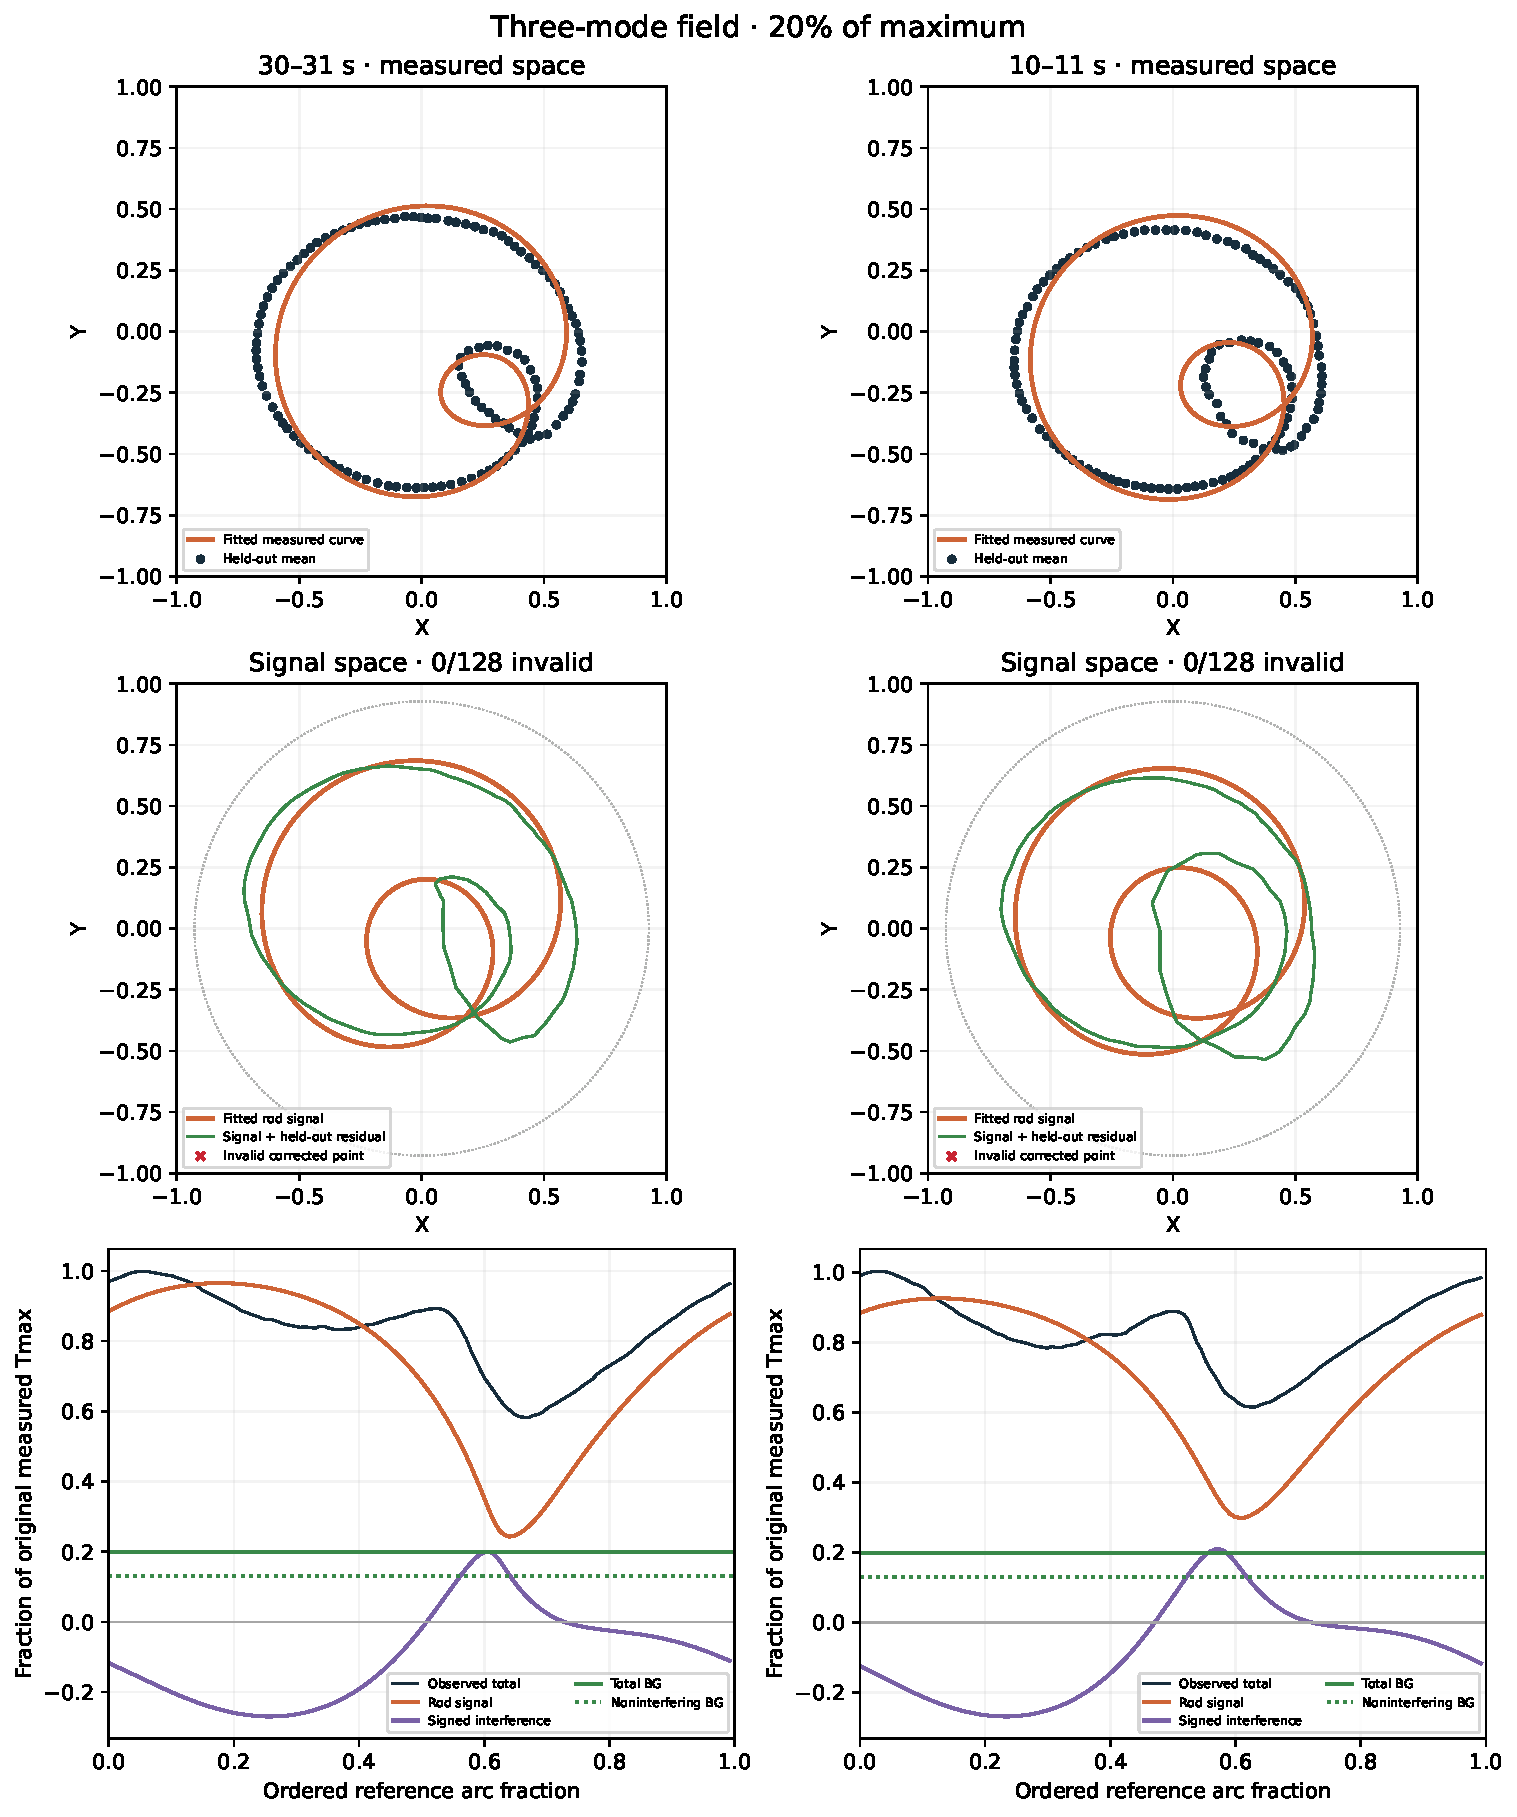
\includegraphics[width=\linewidth,height=.9\textheight,keepaspectratio]{figures/three_20pct.pdf}
\newpage
\subsection{30\% of maximum}\label{case:three:30pct}
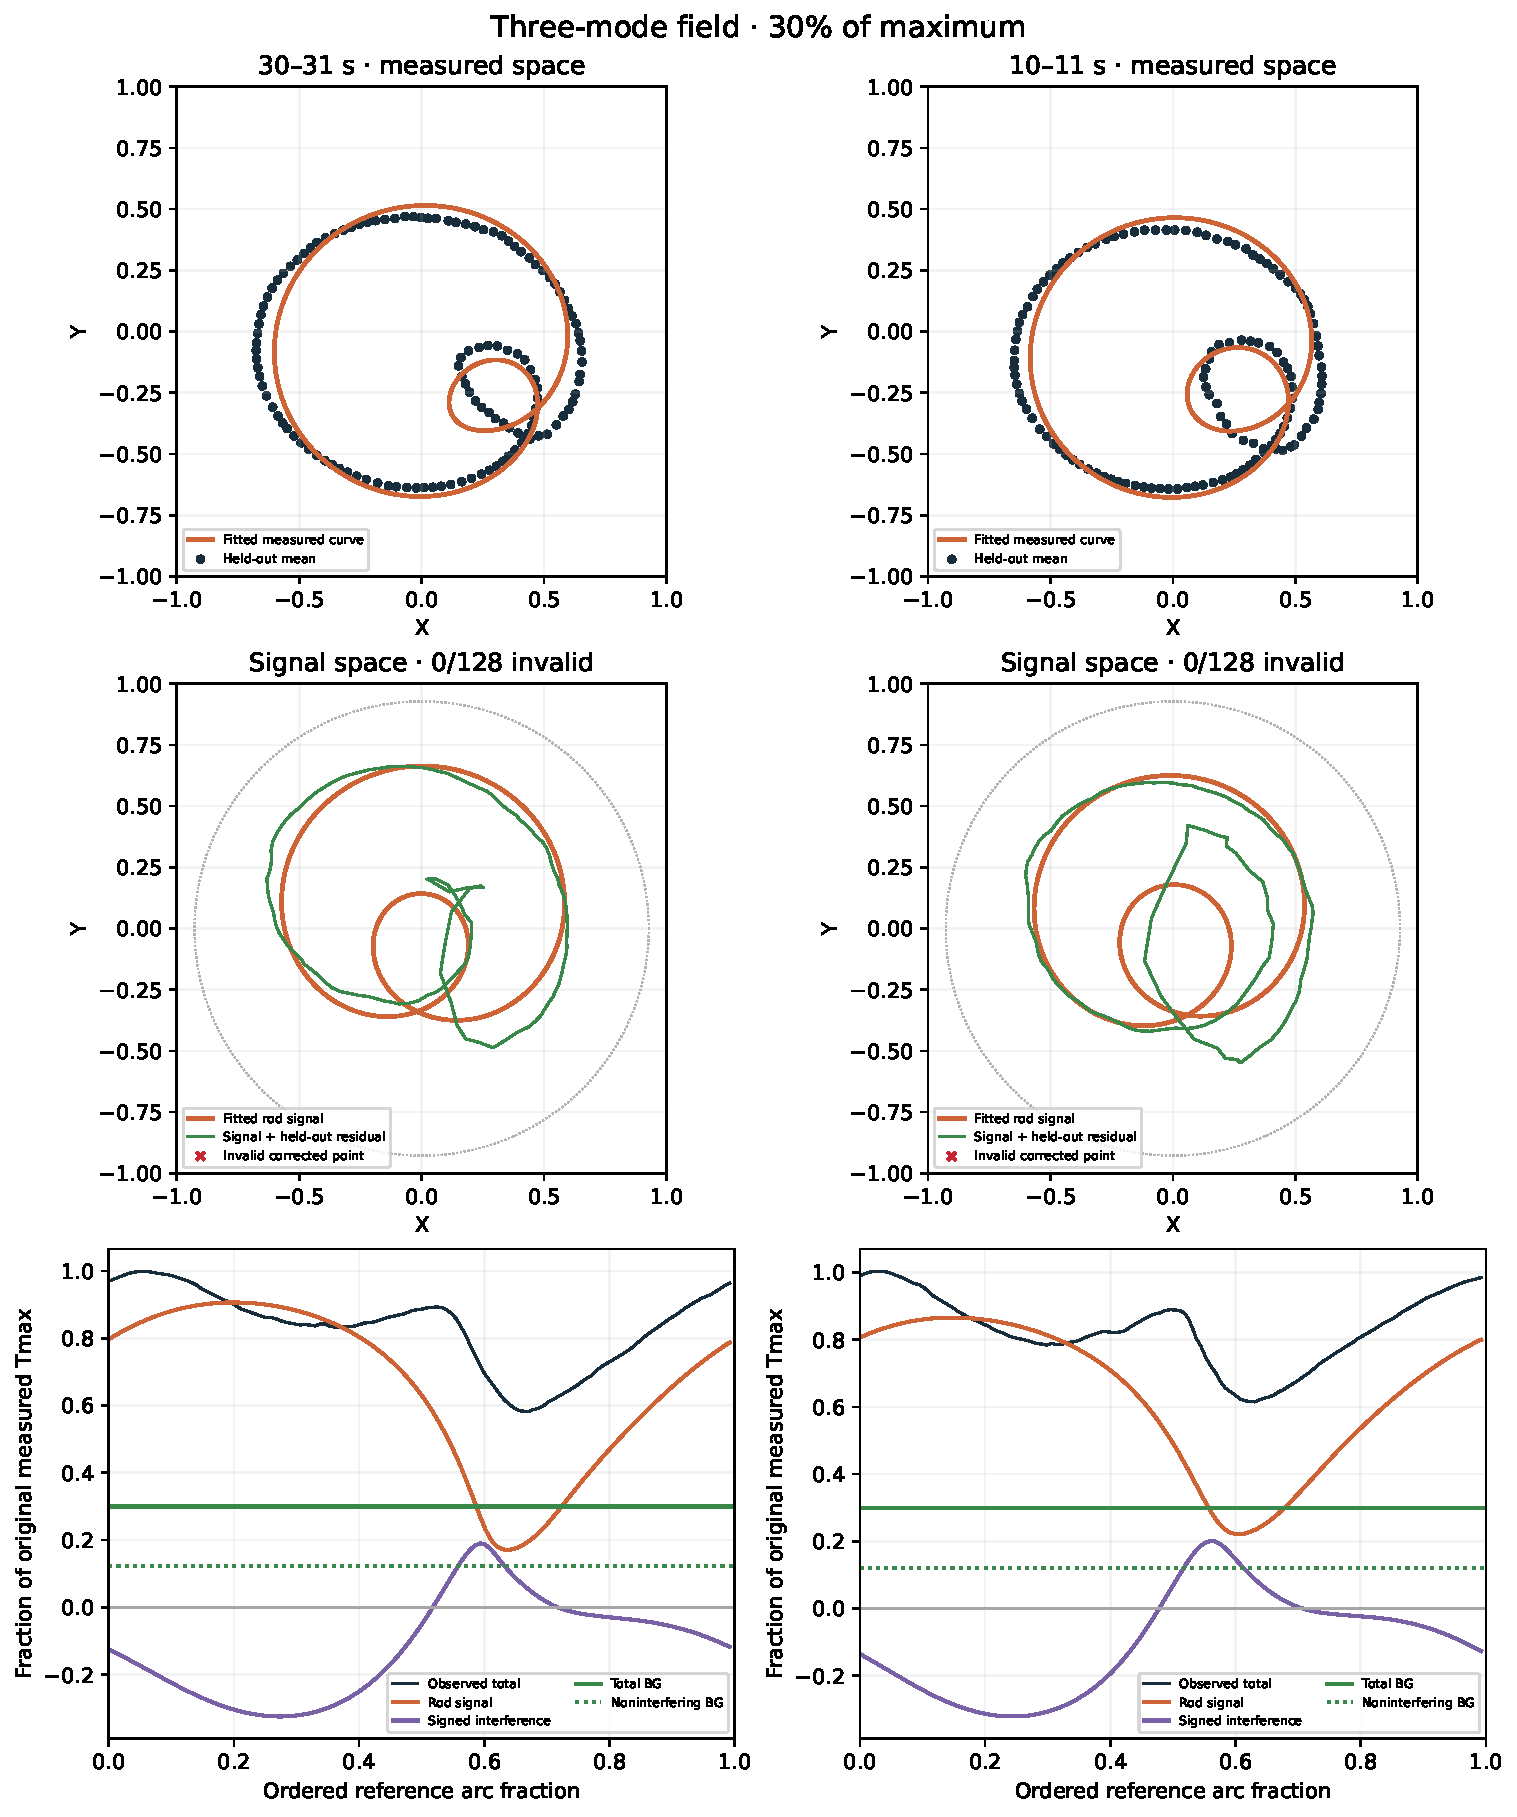
\includegraphics[width=\linewidth,height=.9\textheight,keepaspectratio]{figures/three_30pct.pdf}
\newpage
\subsection{40\% of maximum}\label{case:three:40pct}
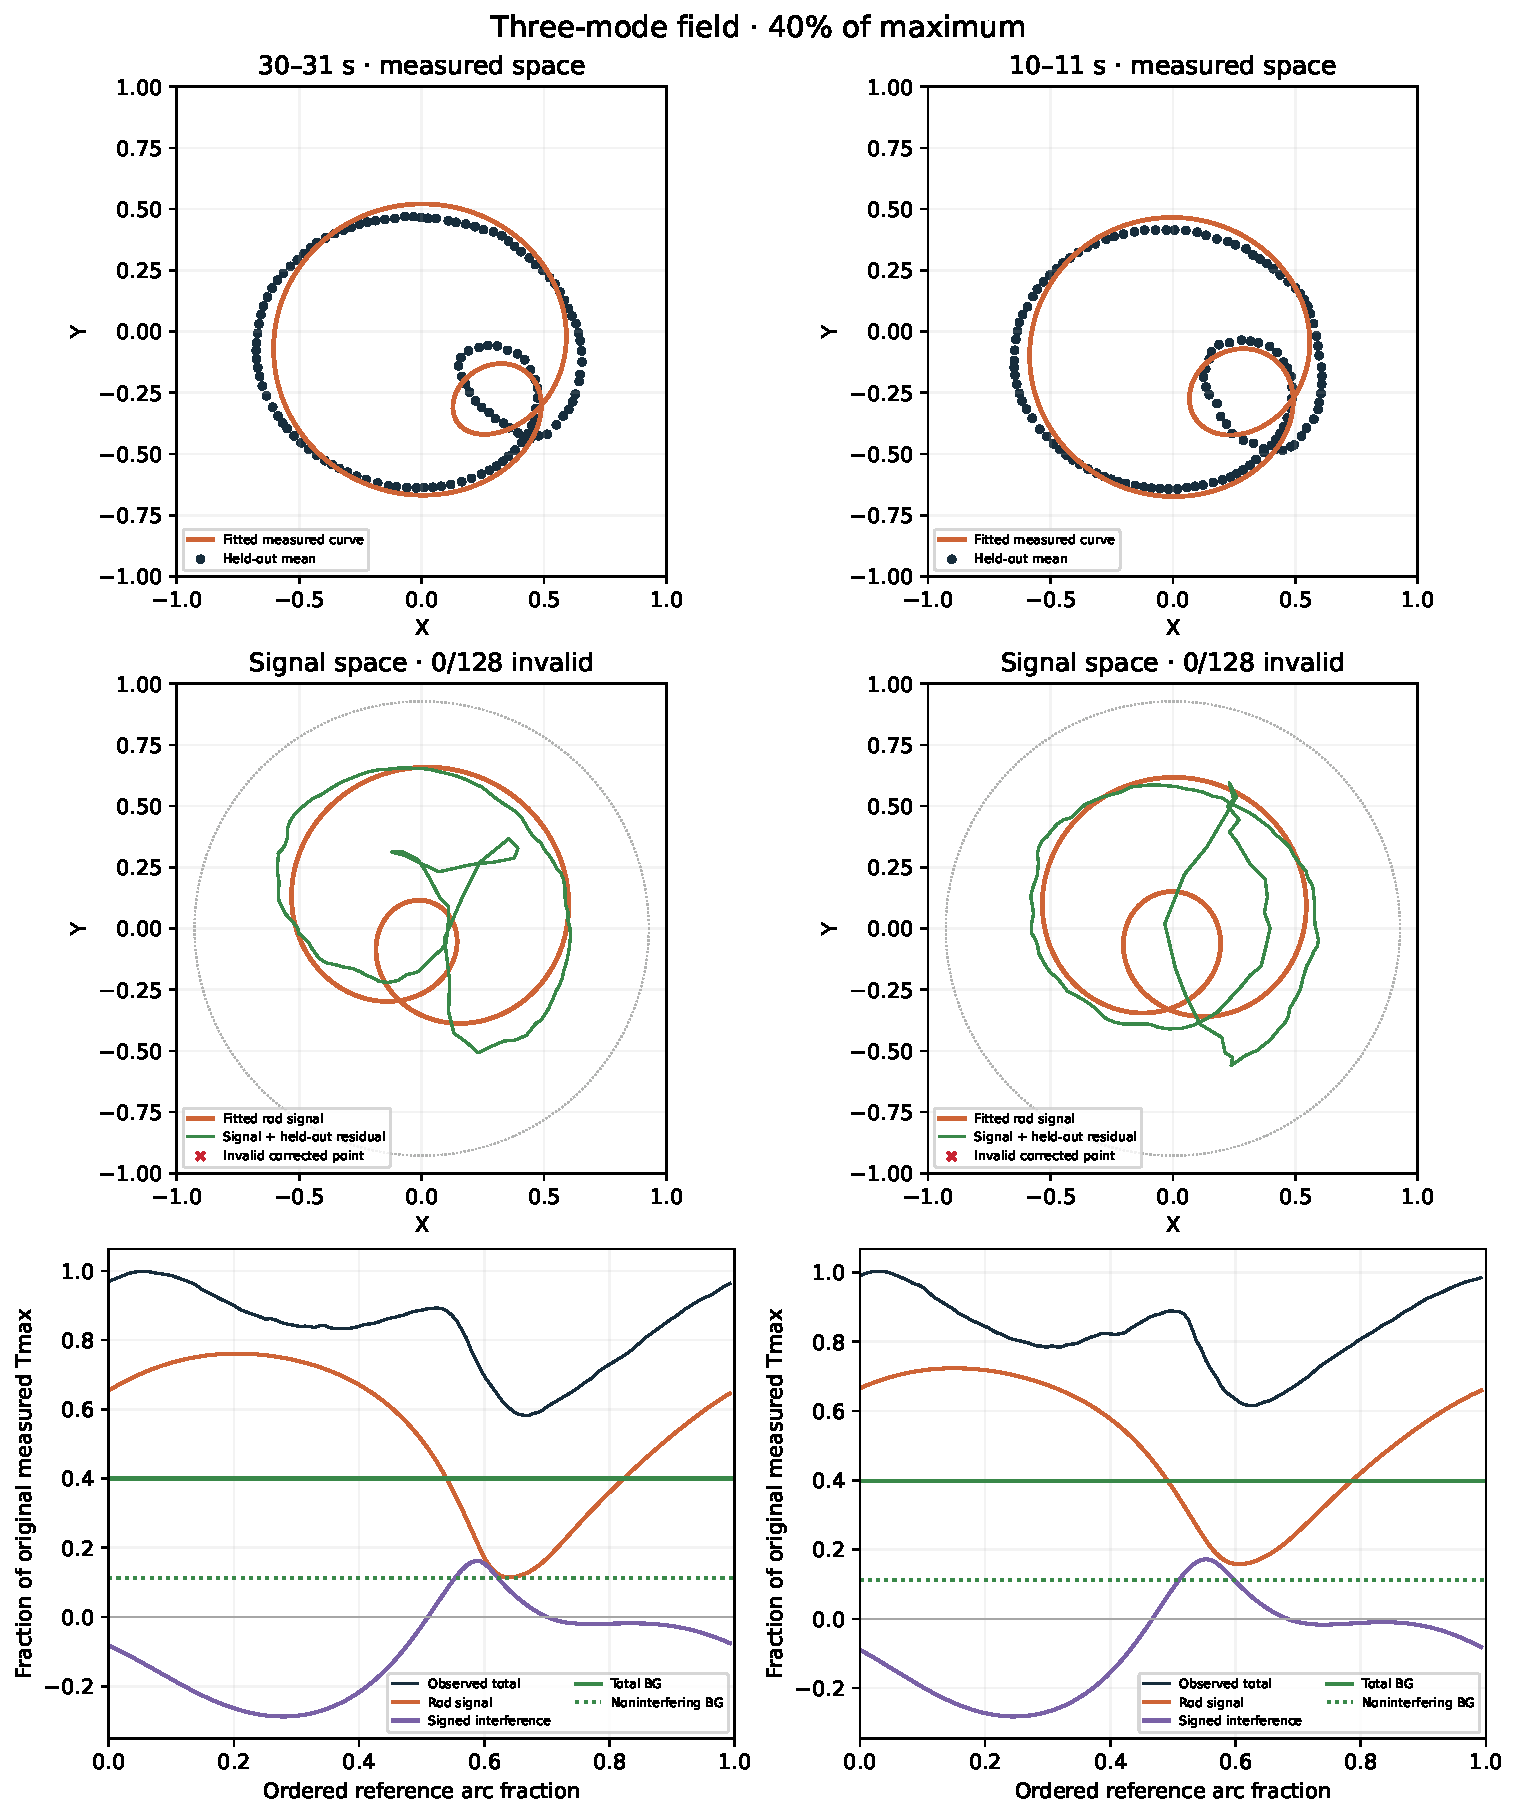
\includegraphics[width=\linewidth,height=.9\textheight,keepaspectratio]{figures/three_40pct.pdf}
\newpage
\subsection{50\% of maximum}\label{case:three:50pct}
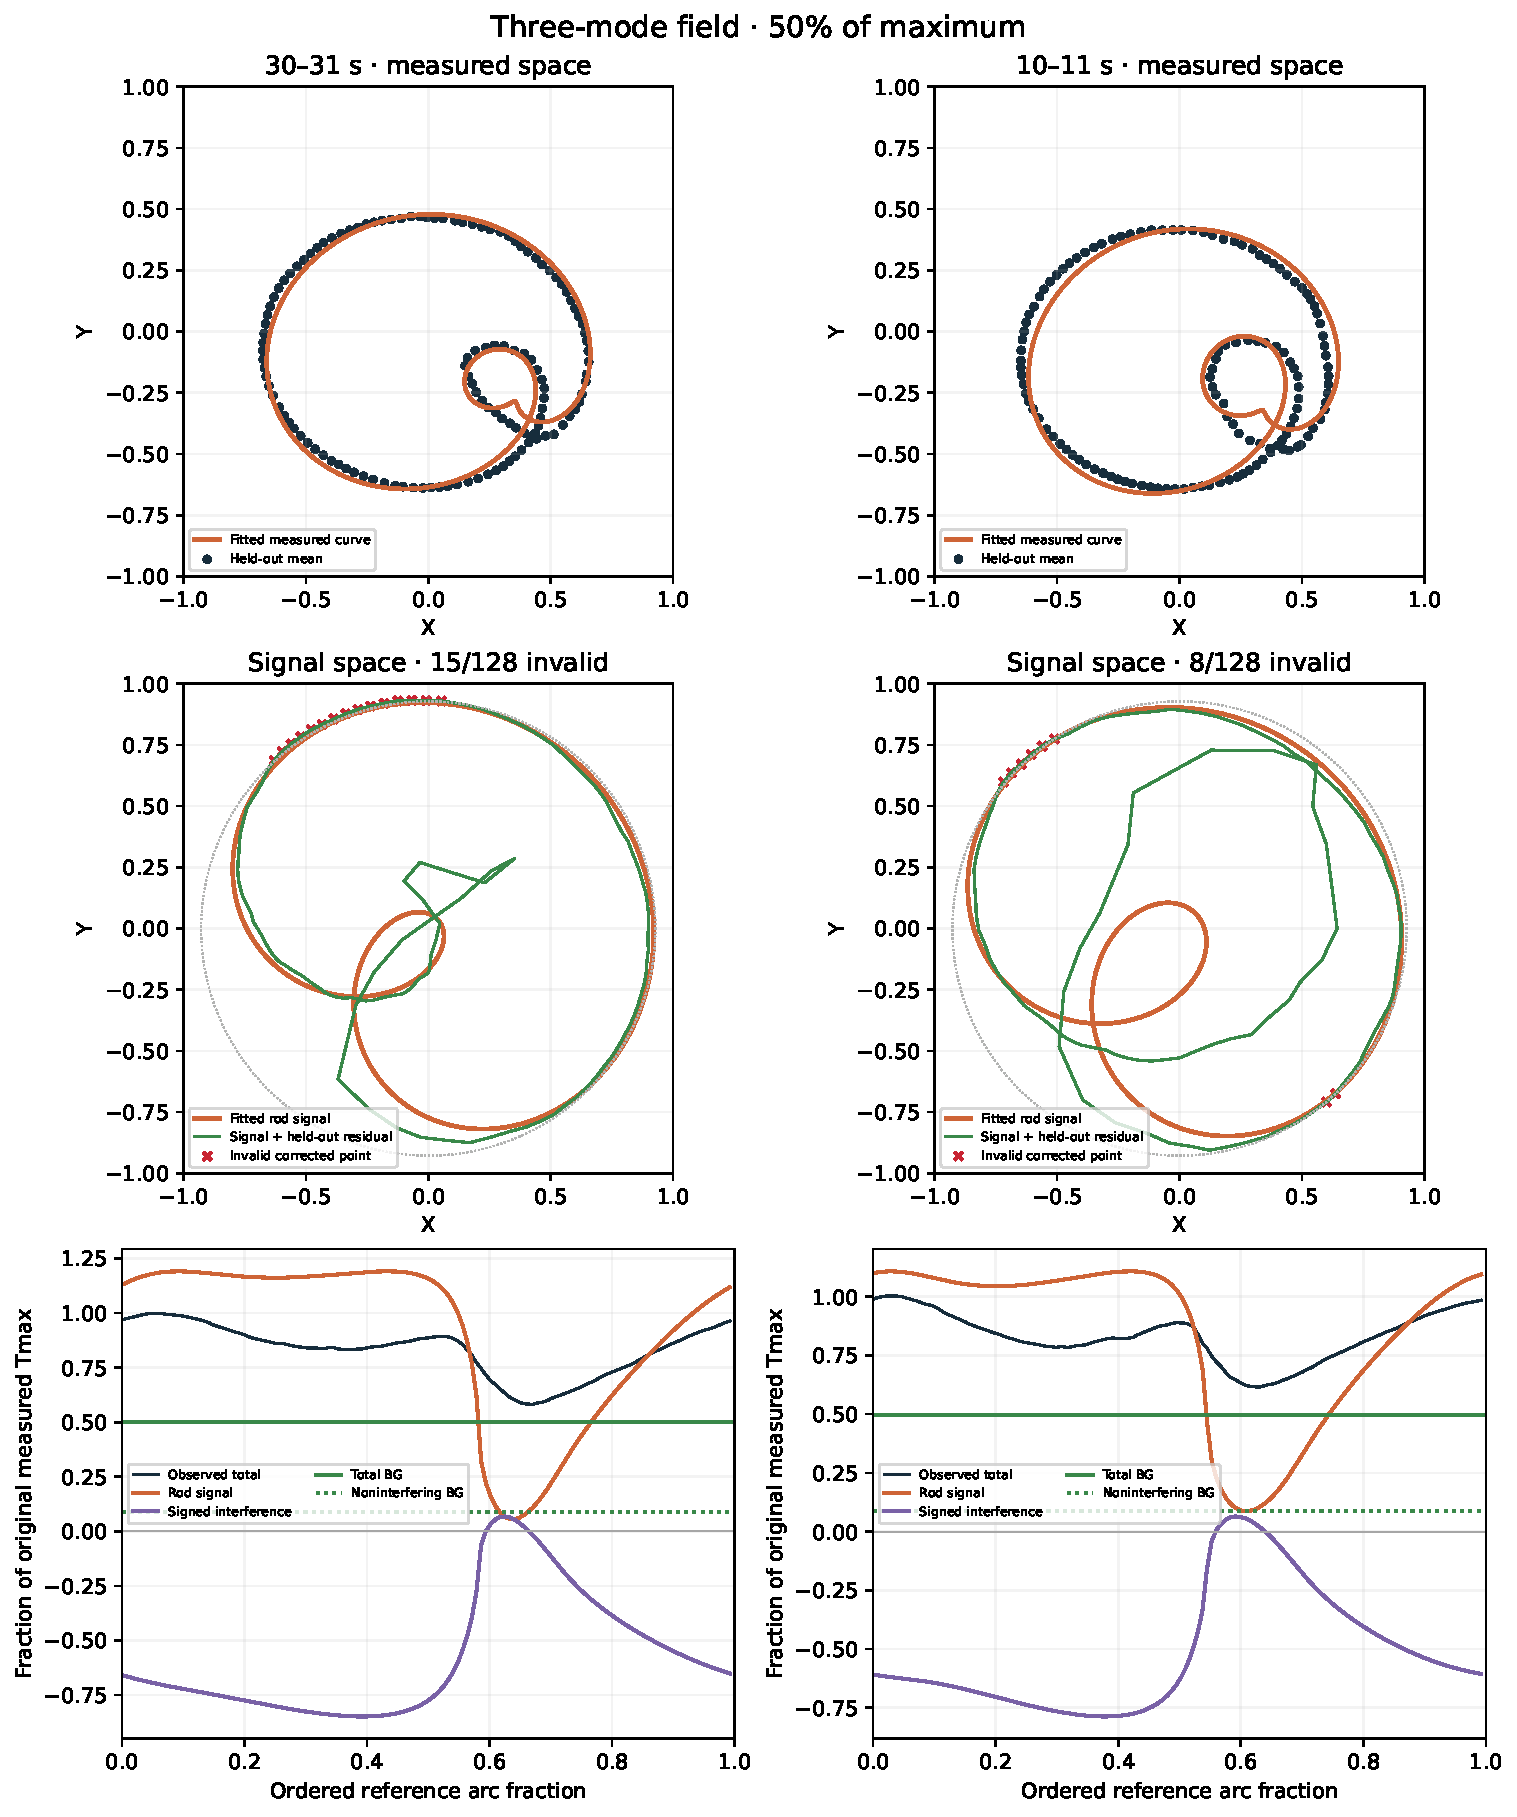
\includegraphics[width=\linewidth,height=.9\textheight,keepaspectratio]{figures/three_50pct.pdf}
\newpage
\subsection{Representative sphere diagnostic: 10\% of maximum}
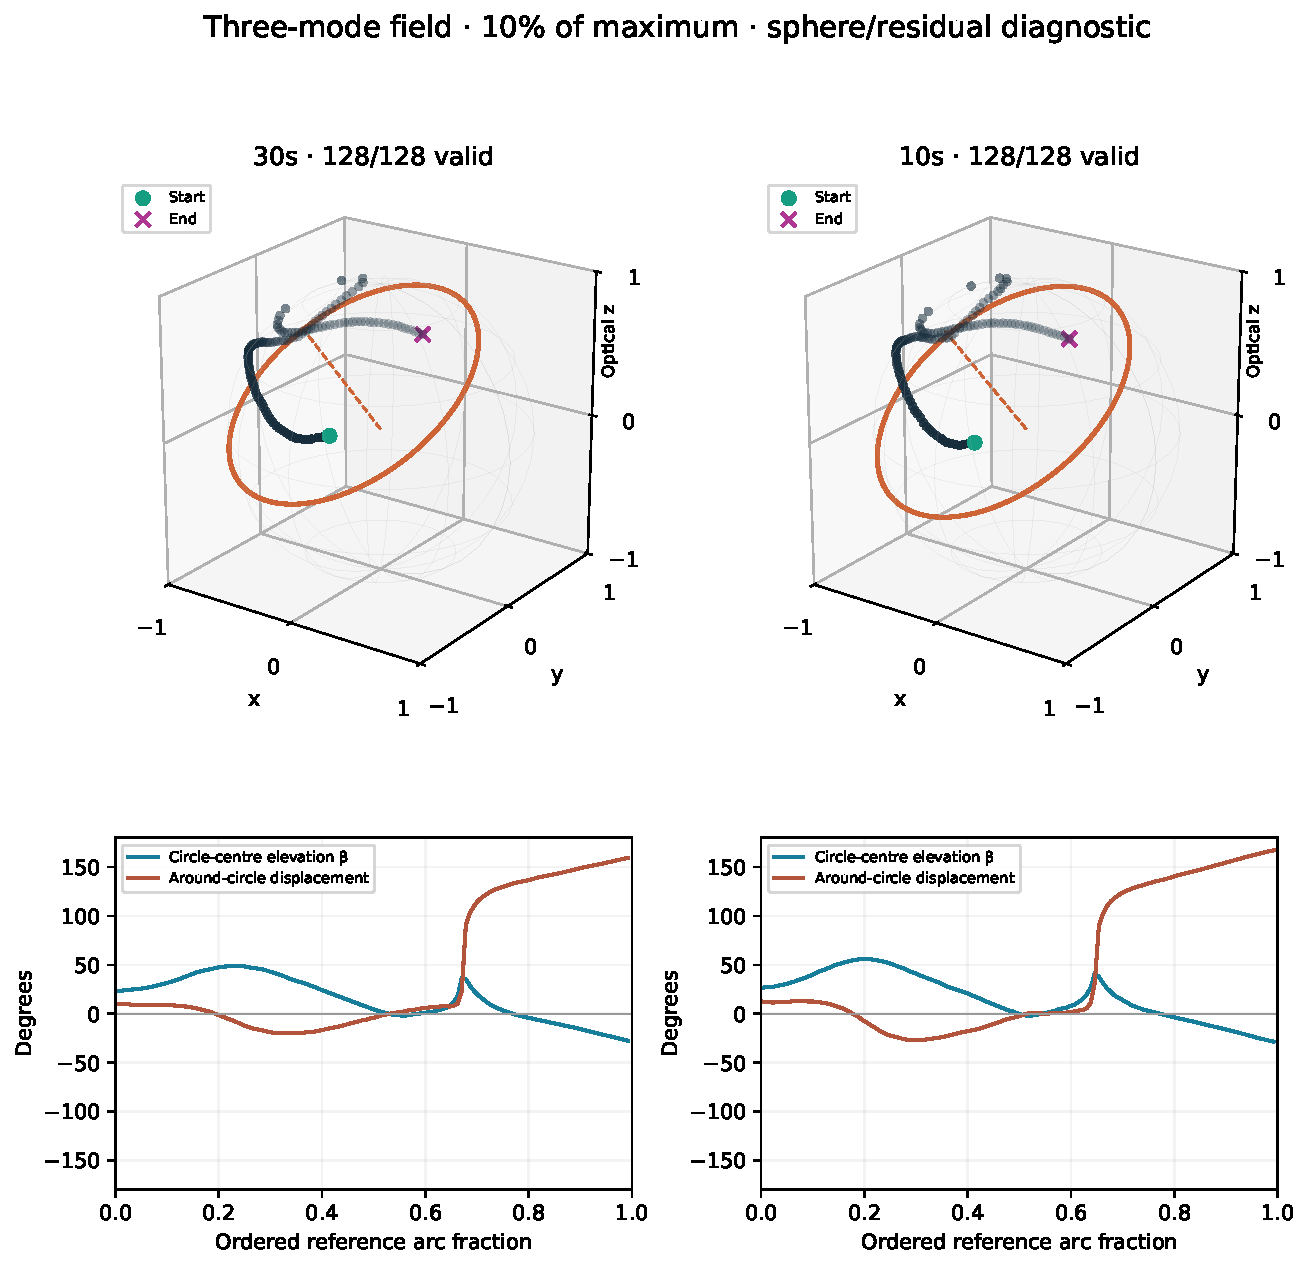
\includegraphics[width=\linewidth,height=.82\textheight,keepaspectratio]{figures/three_sphere.pdf}
30s: 128/128 valid; matched geodesic RMS 79.41$^\circ$; oriented closure mismatch 142.98$^\circ$.\par
10s: 128/128 valid; matched geodesic RMS 85.41$^\circ$; oriented closure mismatch 147.78$^\circ$.\par
\newpage
\subsection{Local cone-referenced angular residual: 10\% of maximum}\label{local:three}
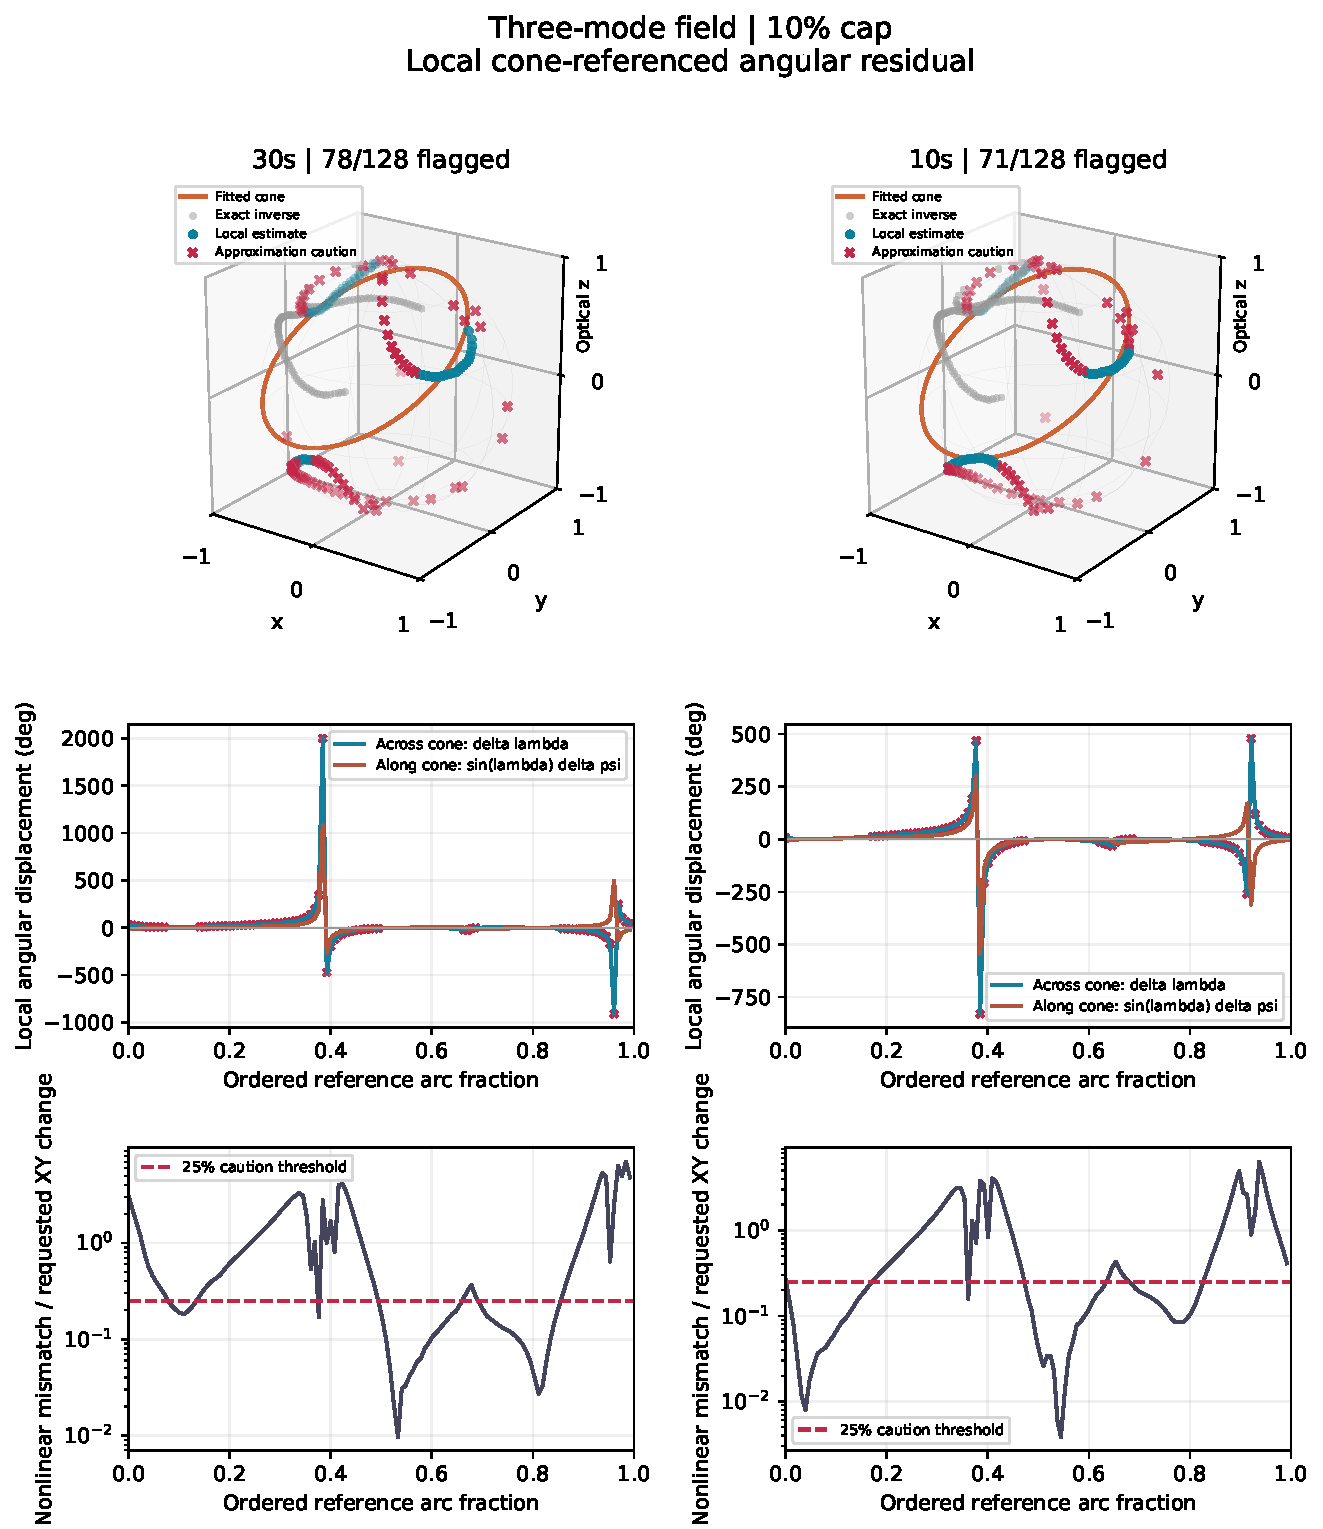
\includegraphics[width=\linewidth,height=.86\textheight,keepaspectratio]{local_residual/three.pdf}
30s: local angular RMS 235.38$^\circ$; 78/128 caution flags; median nonlinear mismatch ratio 0.392.\par
10s: local angular RMS 125.30$^\circ$; 71/128 caution flags; median nonlinear mismatch ratio 0.261.\par
\newpage
\section{Five-mode field}
\[\mathbf{E}_b=\sum_{m=1}^{5}b_m\mathbf{U}_m,\qquad I_i=S_i+I_{\mathrm{int},i}+B_i.\]
Modes comprise two uniform-polarization fields and three dipole-derived vector fields, orthonormalized. Five complex coefficients plus noninterfering Stokes background: thirteen shared background parameters and ten local parameters. Spatial shape, polarization and phase are fixed throughout both windows; only the signal direction changes.
\textbf{Total fitted continuous parameters across both windows: 23.} The three pre-estimated gain adjustments are additional calibration parameters, held fixed here.
\begin{longtable}{llrrrrrr}\toprule
Budget & Window & BG\% & Meas.RMS & Signal RMS & Bad(train/test) & Max $r$ & Conv.\\\midrule\endhead
uncapped & 30s & 56.3 & 0.0064 & 0.0278 & 11/21 & 0.936 & yes \\
uncapped & 10s & 56.1 & 0.0104 & 0.0303 & 6/15 & 0.942 & yes \\
5pct & 30s & 5.0 & 0.0327 & 0.0433 & 0/0 & 0.705 & yes \\
5pct & 10s & 5.0 & 0.0347 & 0.0427 & 0/0 & 0.720 & yes \\
10pct & 30s & 10.0 & 0.0249 & 0.0347 & 0/0 & 0.673 & yes \\
10pct & 10s & 10.0 & 0.0272 & 0.0352 & 0/0 & 0.694 & yes \\
20pct & 30s & 20.0 & 0.0160 & 0.0237 & 0/0 & 0.754 & yes \\
20pct & 10s & 19.9 & 0.0184 & 0.0267 & 0/0 & 0.710 & yes \\
30pct & 30s & 30.0 & 0.0126 & 0.0223 & 0/0 & 0.753 & yes \\
30pct & 10s & 29.9 & 0.0155 & 0.0263 & 0/0 & 0.695 & yes \\
40pct & 30s & 40.0 & 0.0103 & 0.0208 & 0/0 & 0.823 & yes \\
40pct & 10s & 39.8 & 0.0139 & 0.0263 & 0/0 & 0.767 & yes \\
50pct & 30s & 50.0 & 0.0063 & 0.0177 & 11/18 & 0.940 & yes \\
50pct & 10s & 49.8 & 0.0113 & 0.0263 & 7/13 & 0.937 & yes \\
\bottomrule\end{longtable}
\begin{longtable}{llrrrr}\toprule
Budget & Window & Signal\% range & Cross\% range & Noninterf.BG\% & Fitted folded $\theta$\\\midrule\endhead
uncapped & 30s & 6.2--120.0 & -91.9--0.9 & 5.6 & 13.9--90.0$^\circ$ \\
uncapped & 10s & 8.2--112.9 & -86.0---0.1 & 5.5 & 16.6--89.8$^\circ$ \\
5pct & 30s & 35.4--116.8 & -33.7--19.9 & 0.0 & 26.0--51.1$^\circ$ \\
5pct & 10s & 40.9--112.5 & -33.4--20.4 & 0.0 & 27.9--49.4$^\circ$ \\
10pct & 30s & 31.5--110.0 & -31.1--19.1 & 5.0 & 26.4--54.1$^\circ$ \\
10pct & 10s & 37.3--105.9 & -30.8--19.7 & 5.0 & 28.7--52.3$^\circ$ \\
20pct & 30s & 24.6--98.3 & -28.8--18.7 & 11.9 & 26.2--58.6$^\circ$ \\
20pct & 10s & 30.4--94.2 & -28.6--19.6 & 11.8 & 29.2--56.8$^\circ$ \\
30pct & 30s & 18.2--94.4 & -36.2--15.6 & 9.4 & 23.3--60.4$^\circ$ \\
30pct & 10s & 24.0--90.0 & -35.8--16.6 & 9.4 & 26.8--57.8$^\circ$ \\
40pct & 30s & 13.8--92.0 & -45.1--9.3 & 5.4 & 22.1--68.3$^\circ$ \\
40pct & 10s & 20.1--87.5 & -44.1--9.6 & 5.3 & 26.7--64.8$^\circ$ \\
50pct & 30s & 7.8--111.2 & -77.1--5.0 & 5.1 & 16.2--89.8$^\circ$ \\
50pct & 10s & 10.8--103.2 & -71.2--4.1 & 5.1 & 19.9--89.7$^\circ$ \\
\bottomrule\end{longtable}
\textbf{Per-channel constant background, percent of measured maximum:}
\begin{longtable}{llrrrr}\toprule
Budget & Window & $B_0$ & $B_{90}$ & $B_{45}$ & $B_{135}$\\\midrule\endhead
uncapped & 30s & 18.29 & 9.88 & 10.71 & 17.46\\
uncapped & 10s & 18.20 & 9.84 & 10.66 & 17.38\\
5pct & 30s & 1.46 & 1.04 & 1.21 & 1.29\\
5pct & 10s & 1.45 & 1.04 & 1.21 & 1.28\\
10pct & 30s & 3.72 & 1.28 & 1.67 & 3.33\\
10pct & 10s & 3.71 & 1.27 & 1.66 & 3.31\\
20pct & 30s & 8.42 & 1.58 & 2.96 & 7.04\\
20pct & 10s & 8.38 & 1.58 & 2.94 & 7.01\\
30pct & 30s & 12.14 & 2.86 & 4.95 & 10.05\\
30pct & 10s & 12.08 & 2.85 & 4.92 & 10.01\\
40pct & 30s & 15.16 & 4.84 & 7.32 & 12.68\\
40pct & 10s & 15.09 & 4.82 & 7.28 & 12.63\\
50pct & 30s & 17.12 & 7.88 & 9.22 & 15.78\\
50pct & 10s & 17.04 & 7.85 & 9.18 & 15.71\\
\bottomrule\end{longtable}
\newpage
\subsection{No BG-power cap}\label{case:five:uncapped}
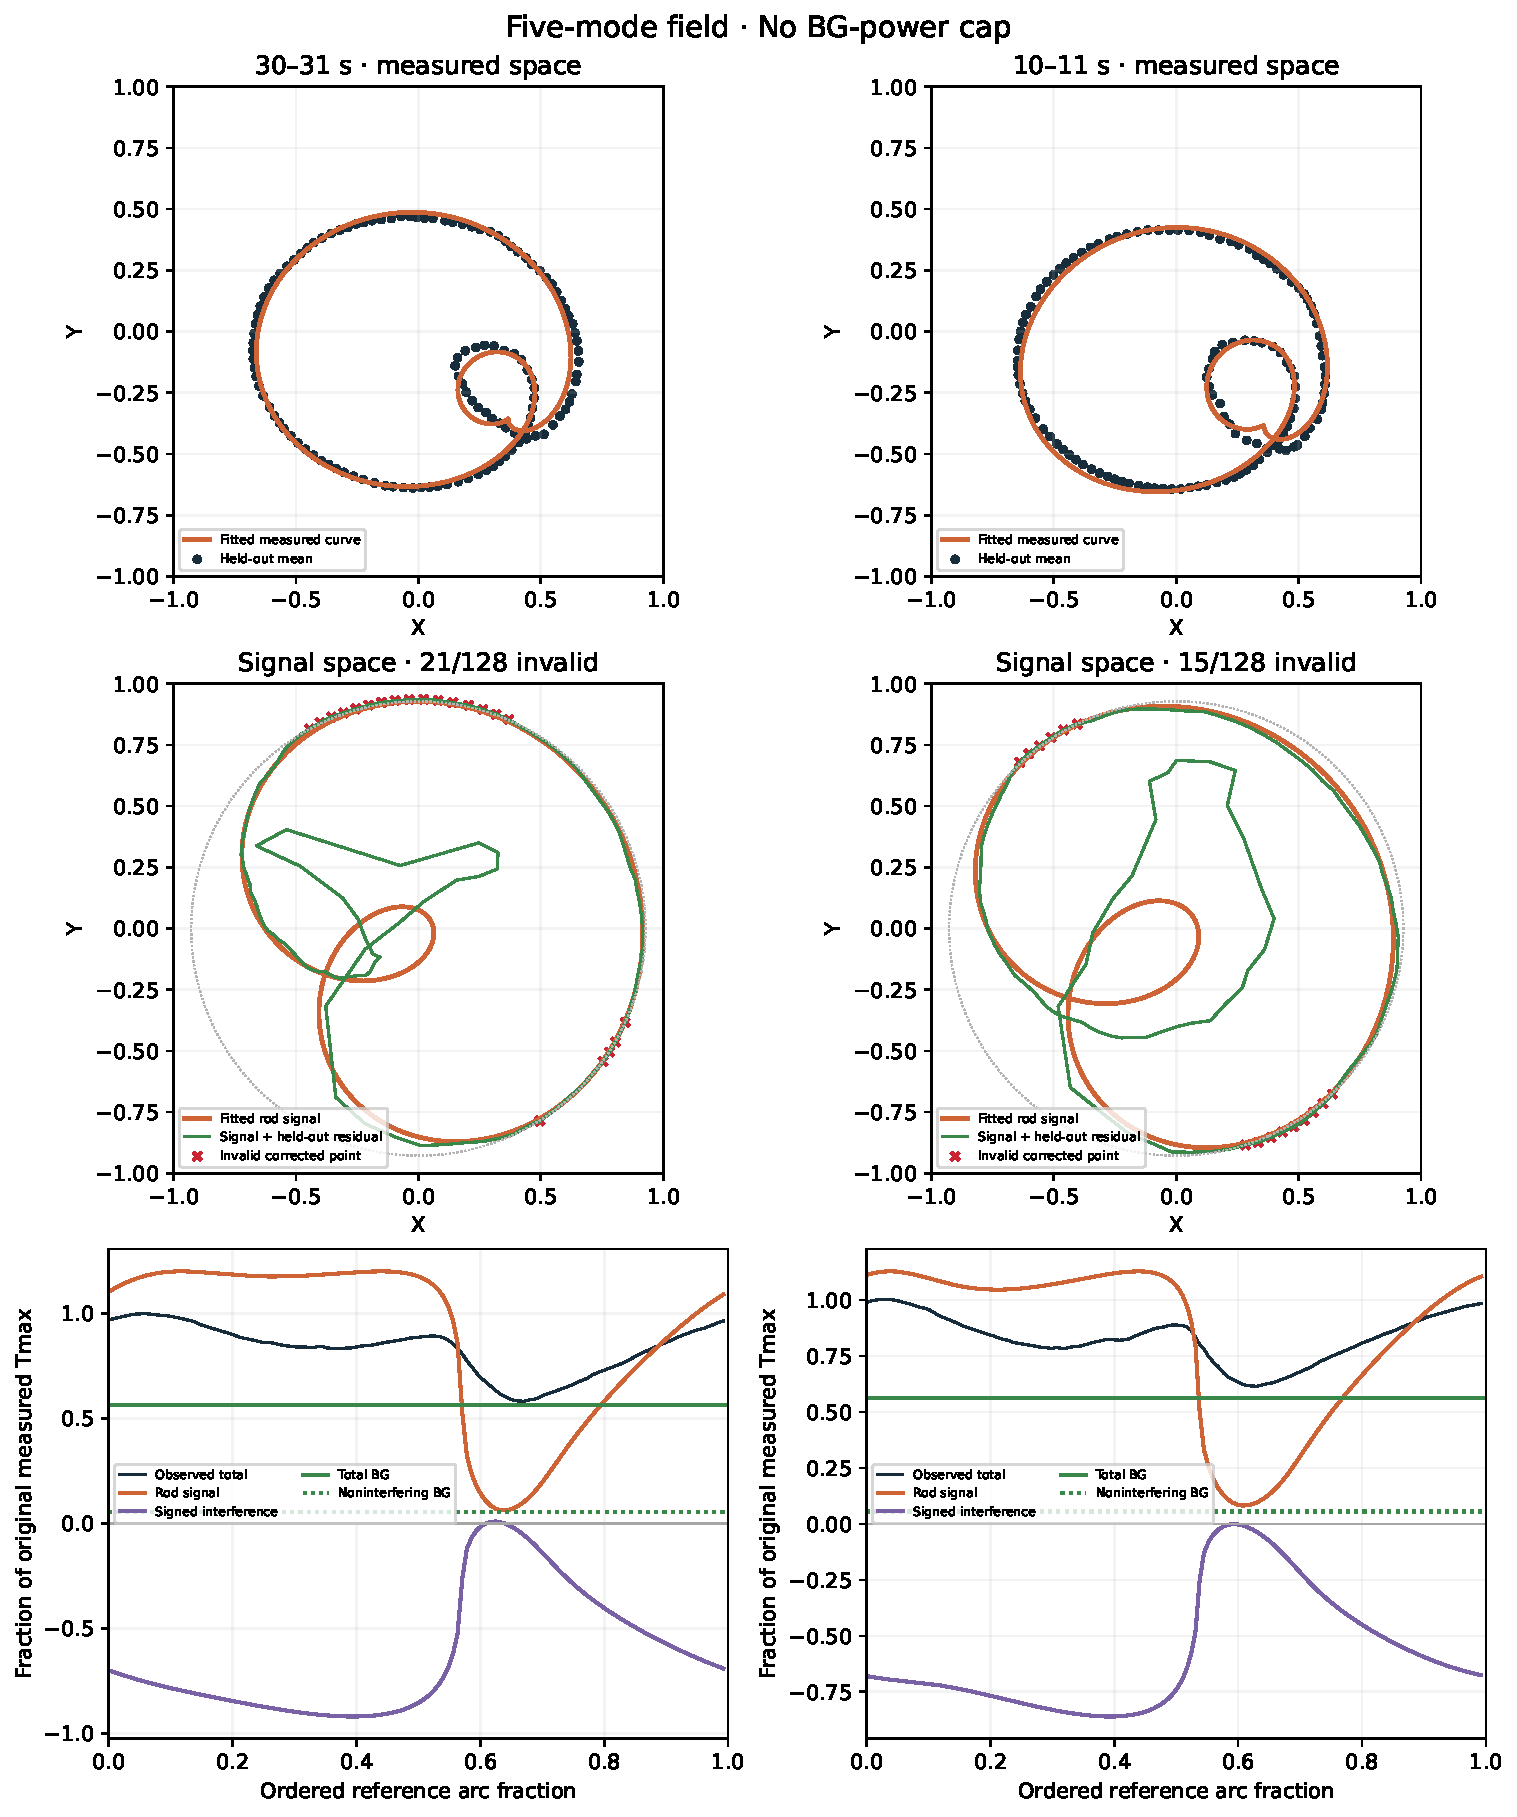
\includegraphics[width=\linewidth,height=.9\textheight,keepaspectratio]{figures/five_uncapped.pdf}
\newpage
\subsection{5\% of maximum}\label{case:five:5pct}
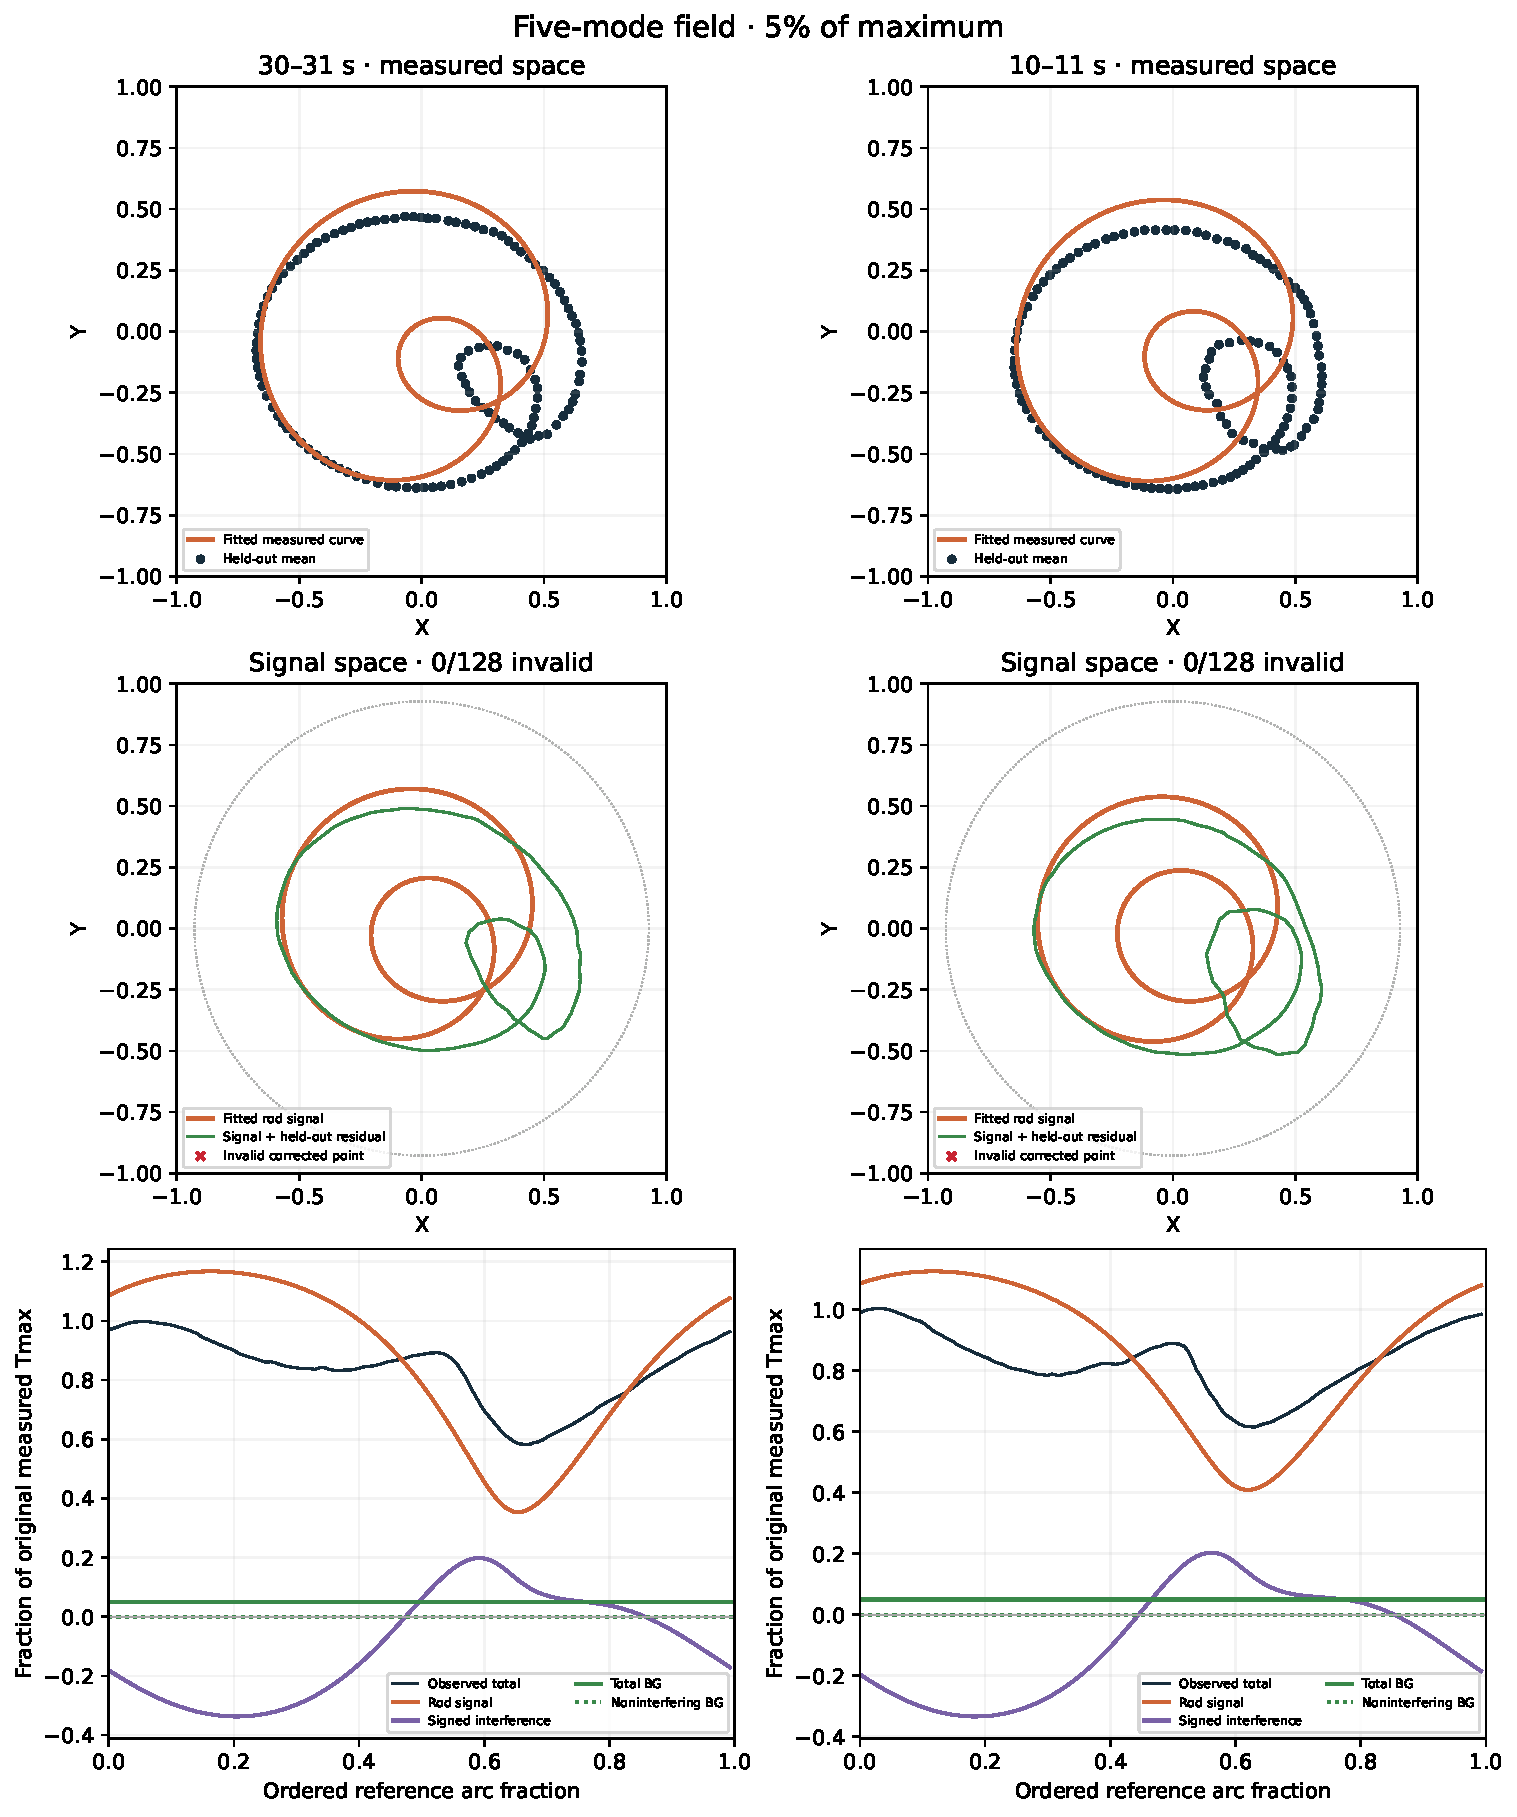
\includegraphics[width=\linewidth,height=.9\textheight,keepaspectratio]{figures/five_5pct.pdf}
\newpage
\subsection{10\% of maximum}\label{case:five:10pct}
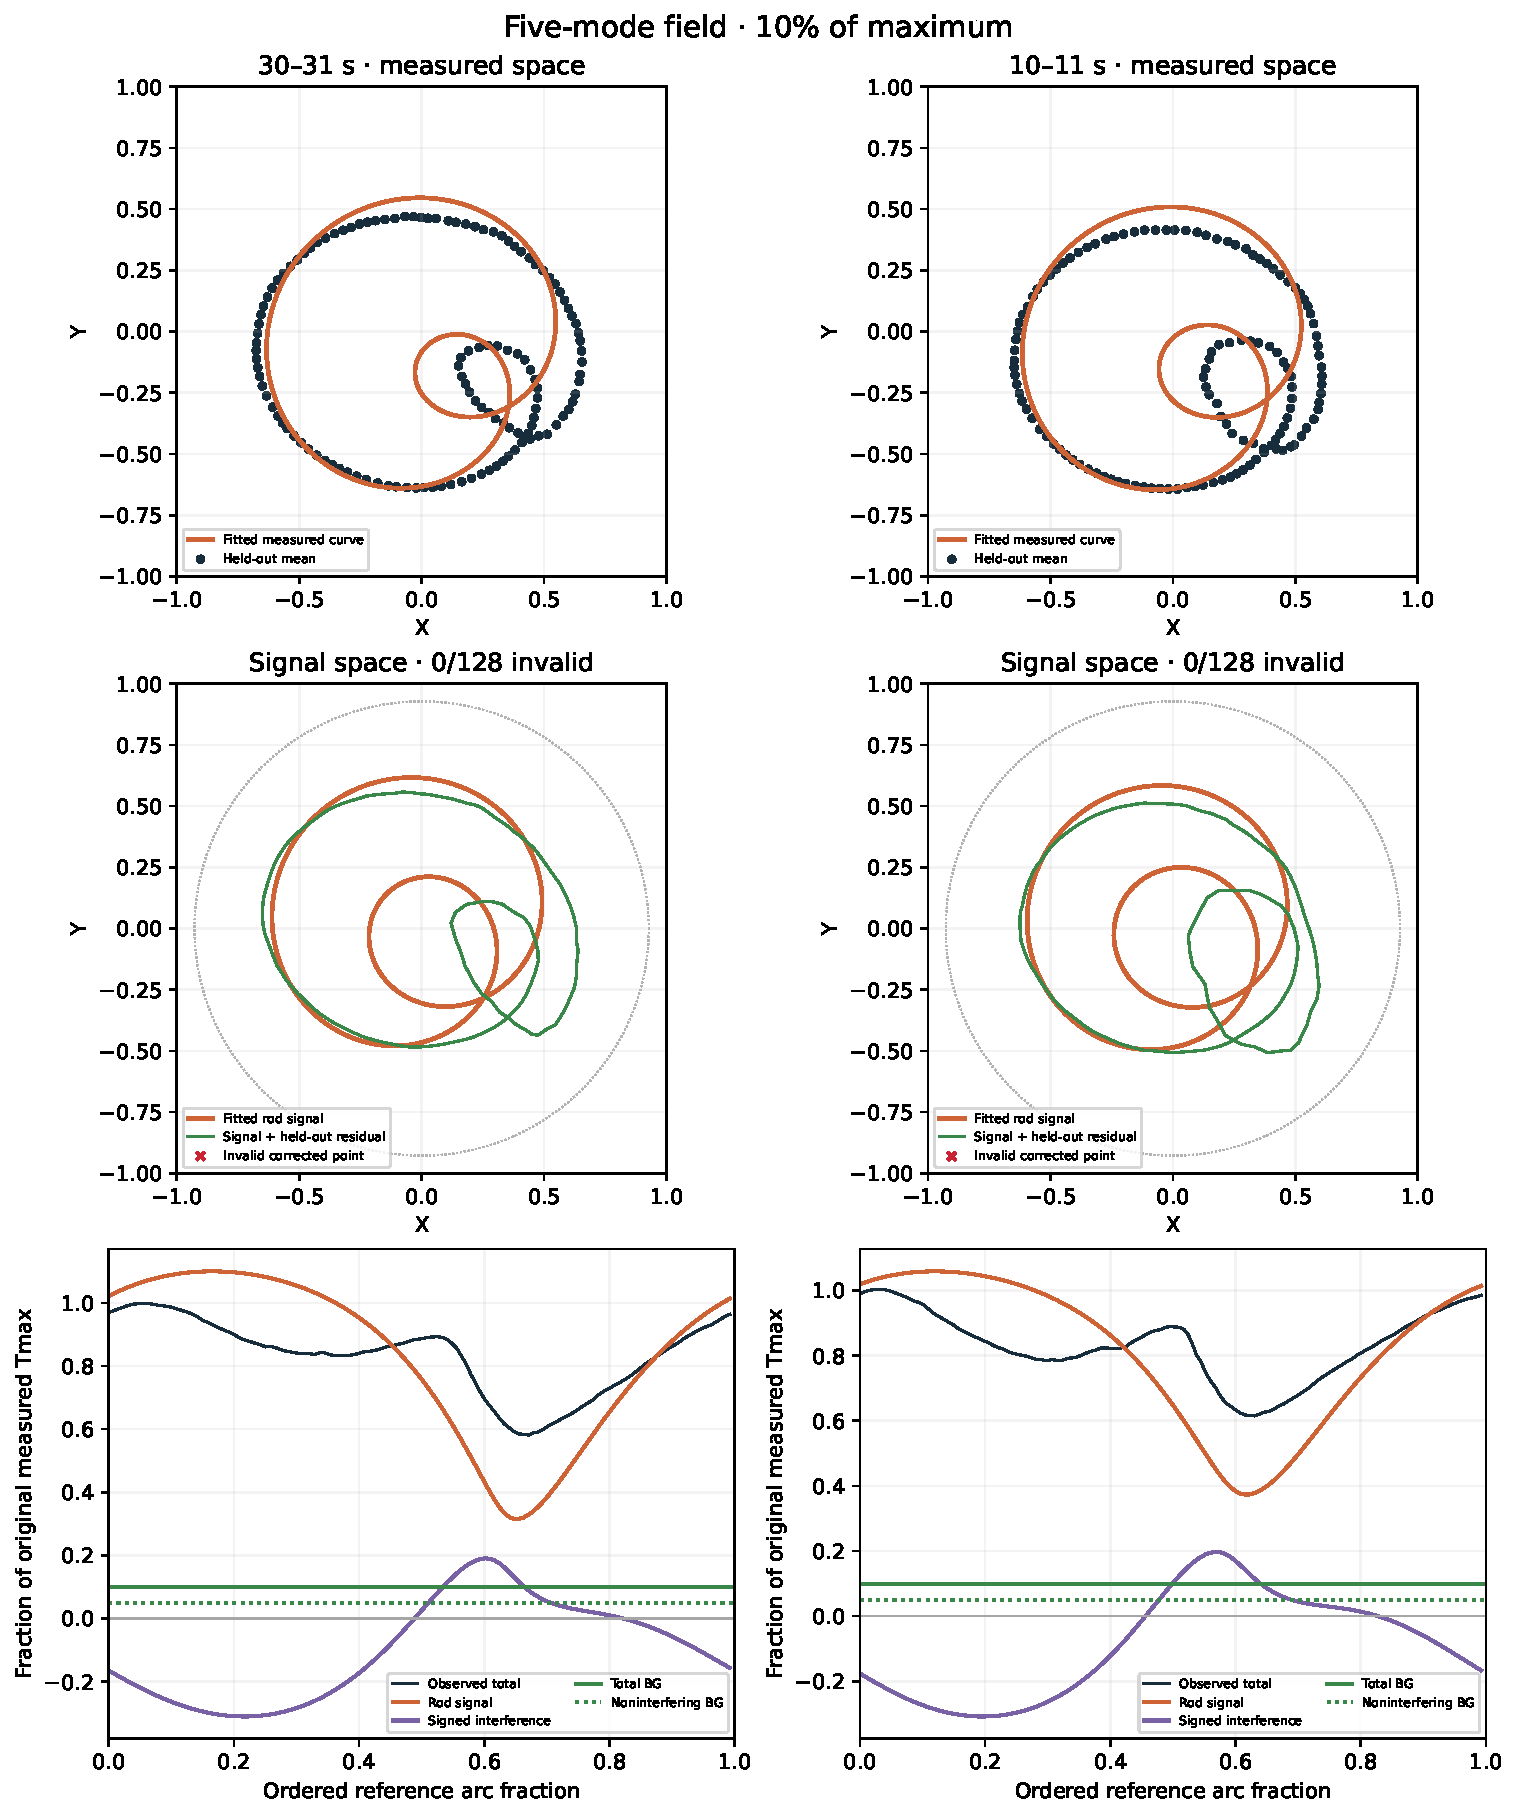
\includegraphics[width=\linewidth,height=.9\textheight,keepaspectratio]{figures/five_10pct.pdf}
\newpage
\subsection{20\% of maximum}\label{case:five:20pct}
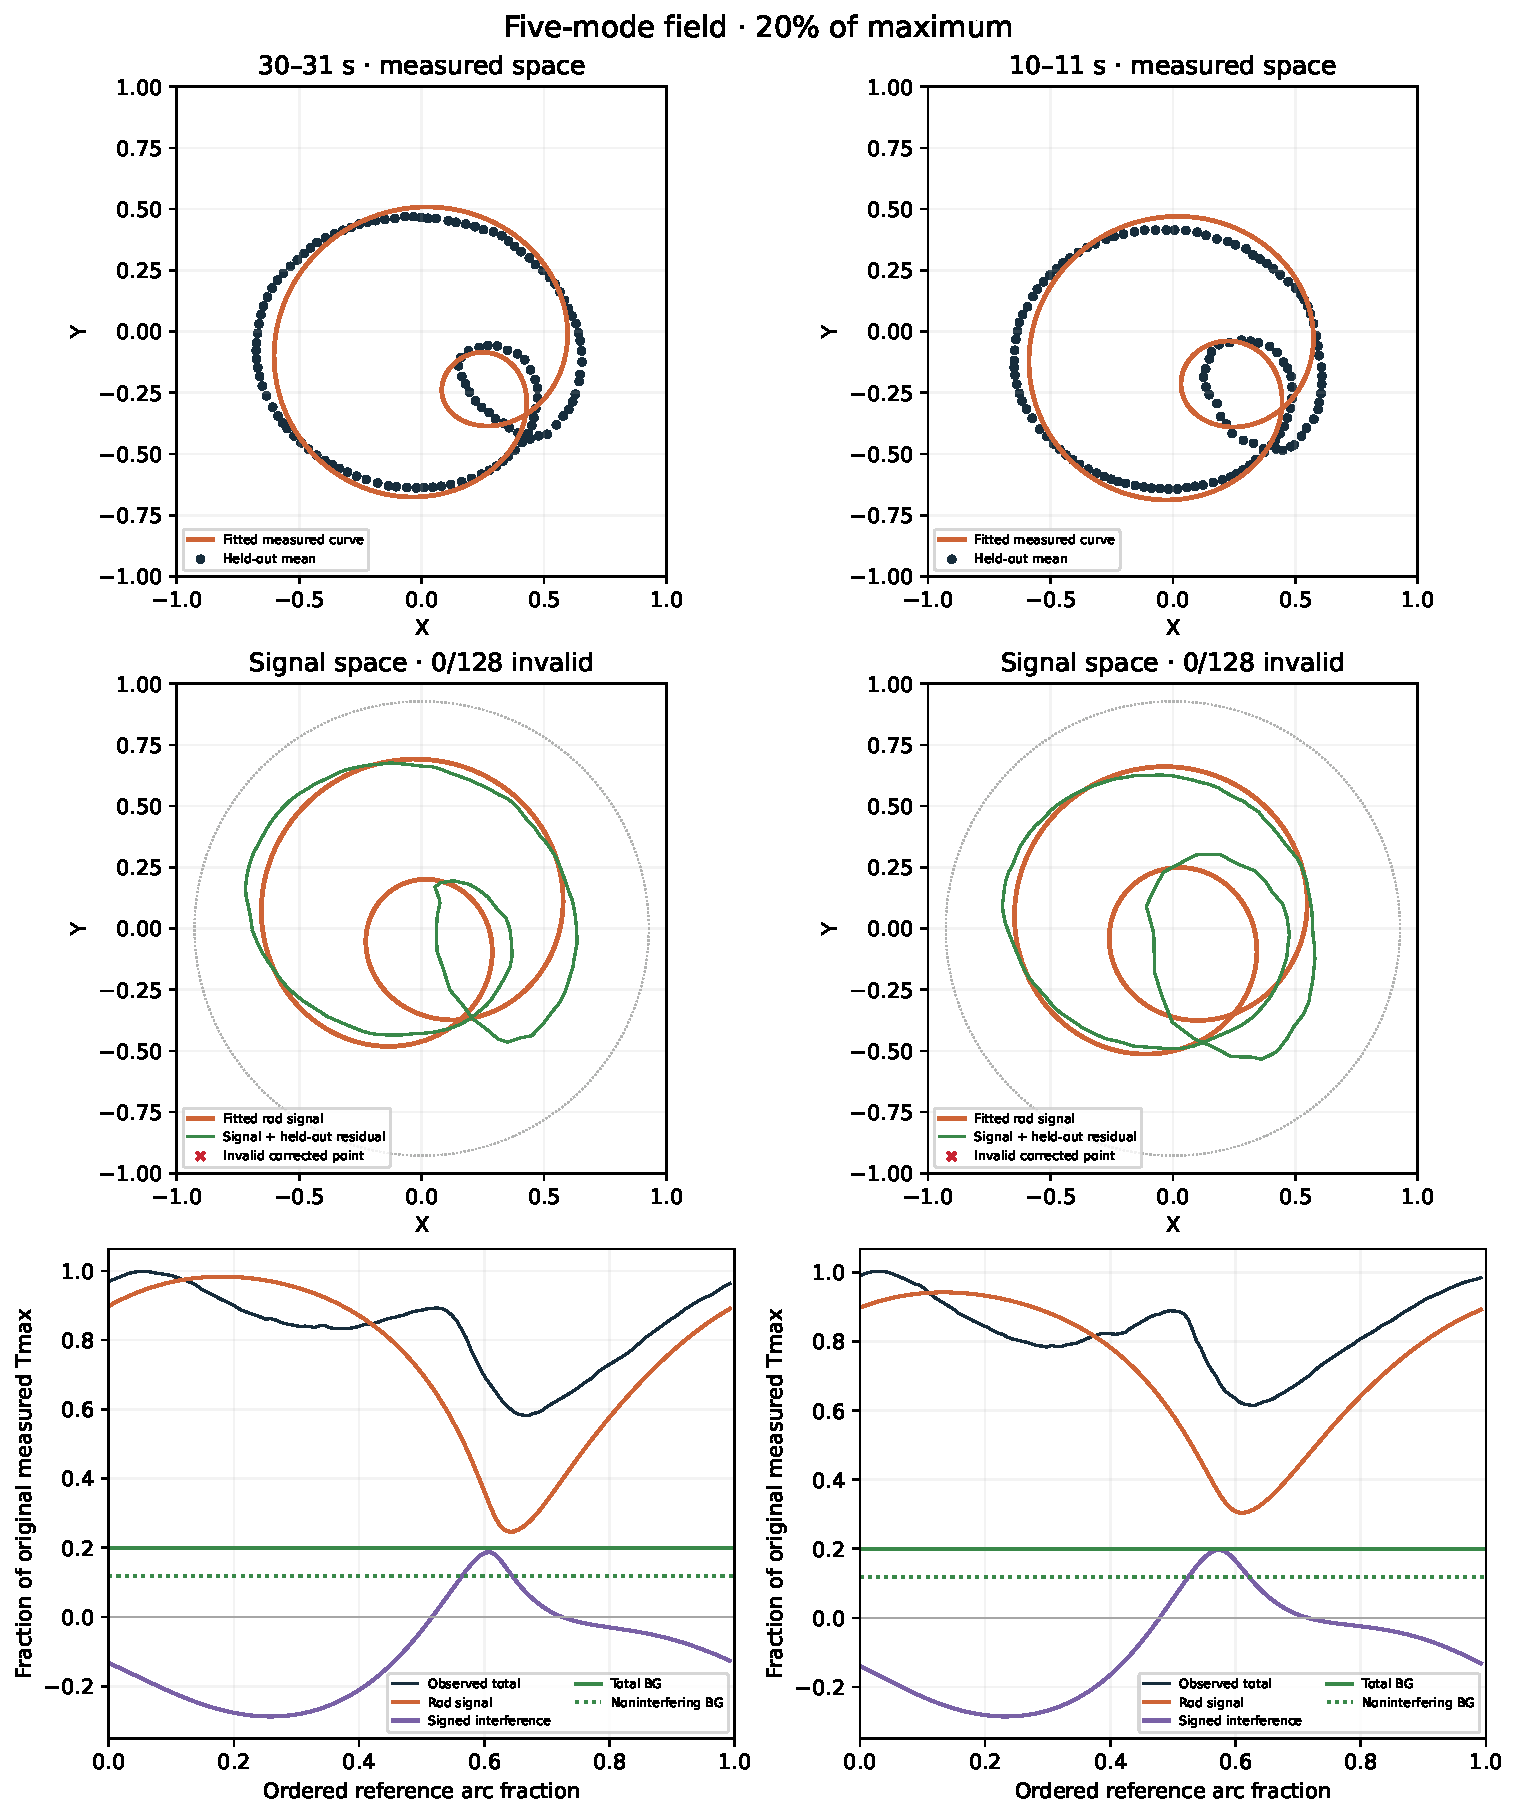
\includegraphics[width=\linewidth,height=.9\textheight,keepaspectratio]{figures/five_20pct.pdf}
\newpage
\subsection{30\% of maximum}\label{case:five:30pct}
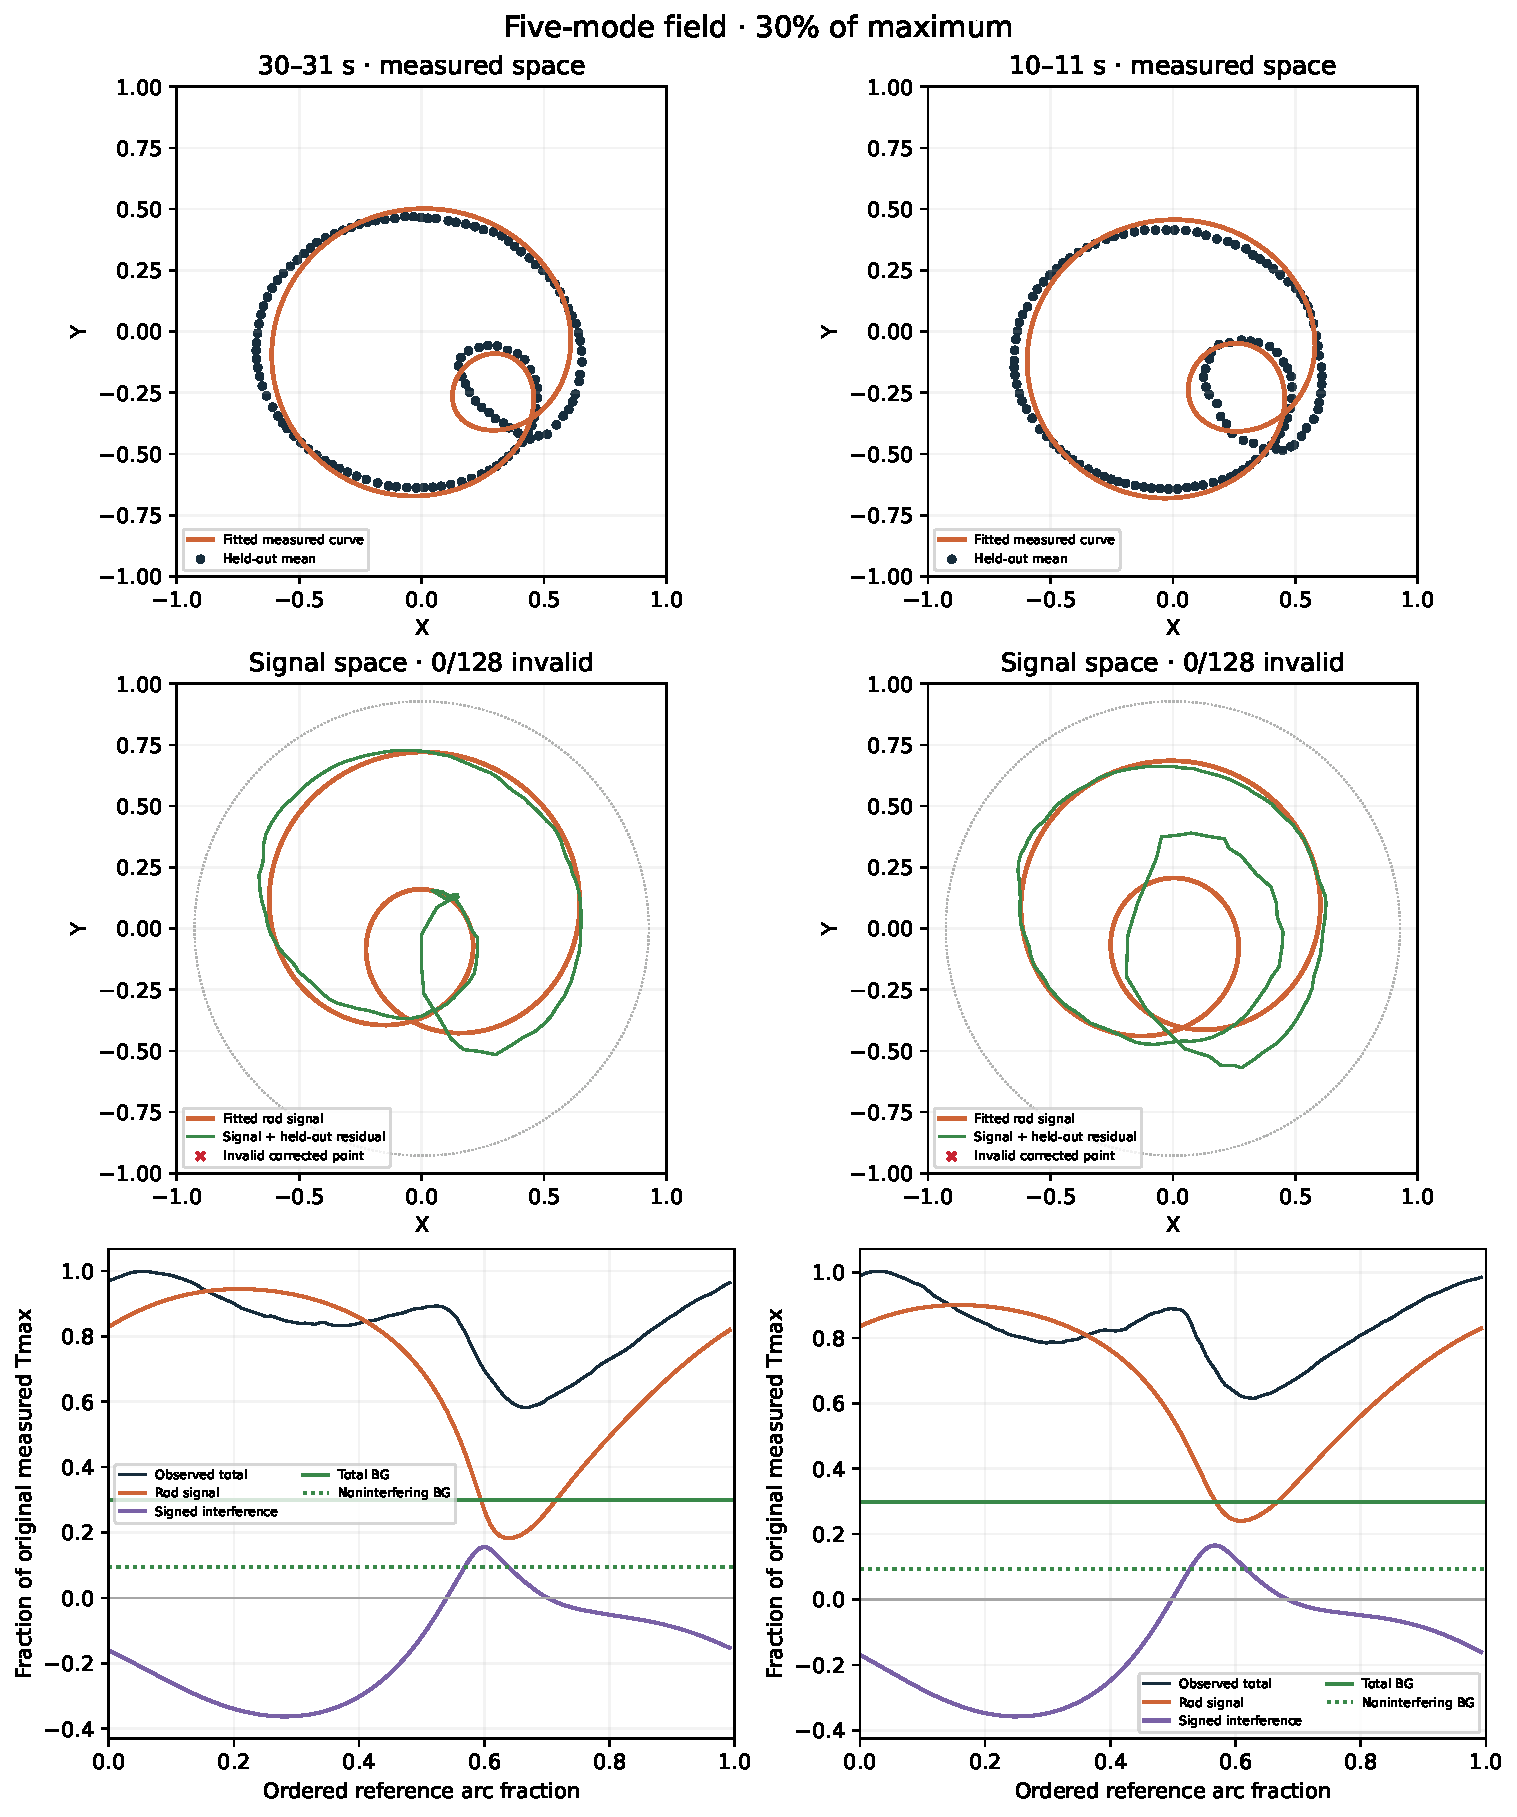
\includegraphics[width=\linewidth,height=.9\textheight,keepaspectratio]{figures/five_30pct.pdf}
\newpage
\subsection{40\% of maximum}\label{case:five:40pct}
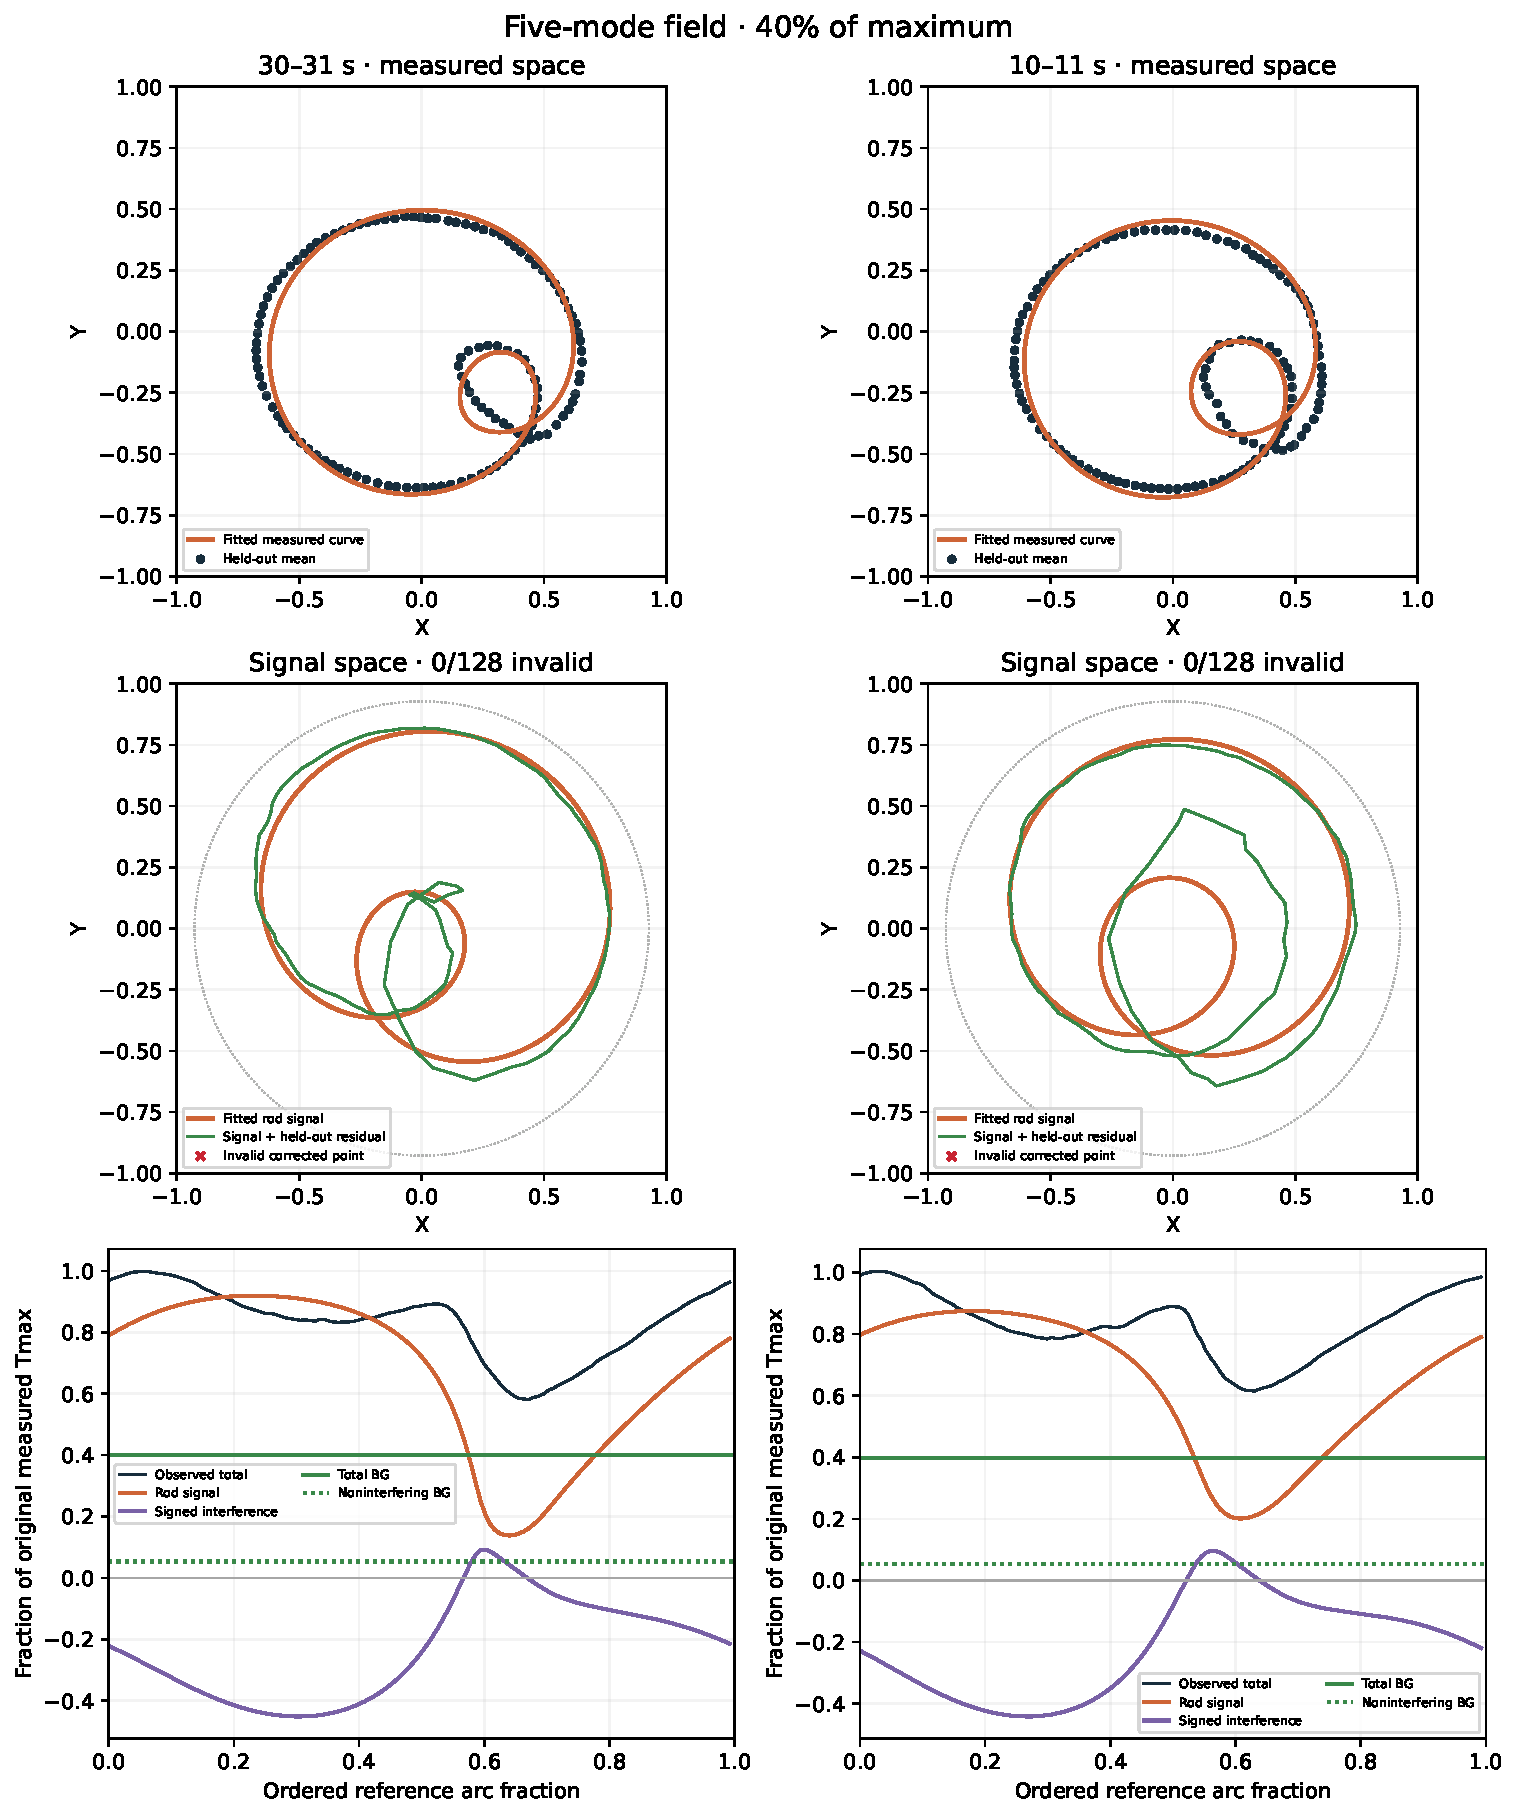
\includegraphics[width=\linewidth,height=.9\textheight,keepaspectratio]{figures/five_40pct.pdf}
\newpage
\subsection{50\% of maximum}\label{case:five:50pct}
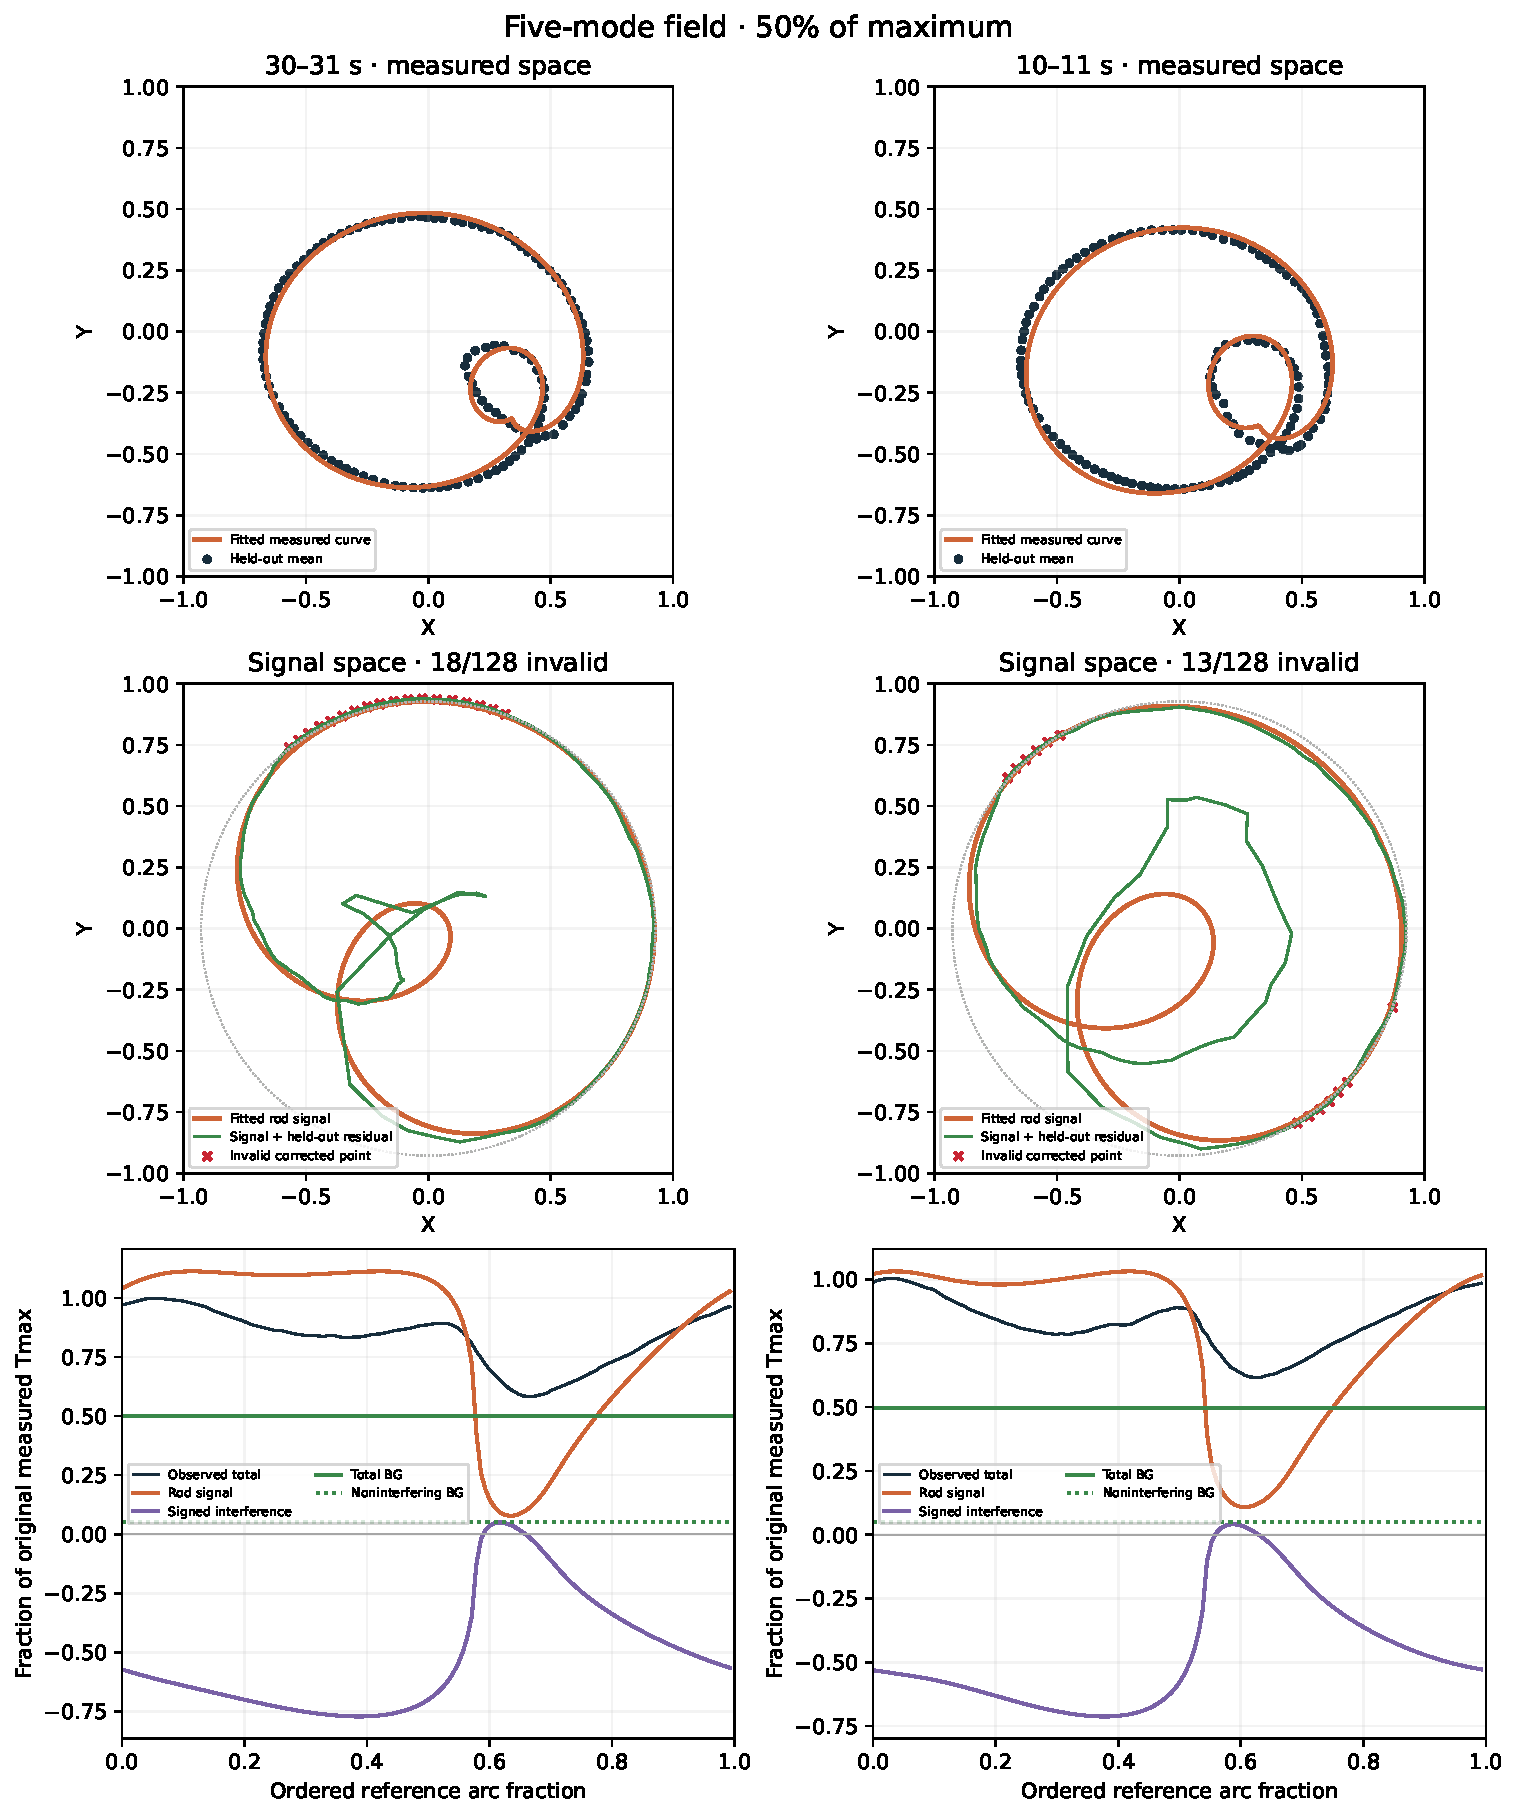
\includegraphics[width=\linewidth,height=.9\textheight,keepaspectratio]{figures/five_50pct.pdf}
\newpage
\subsection{Representative sphere diagnostic: 10\% of maximum}
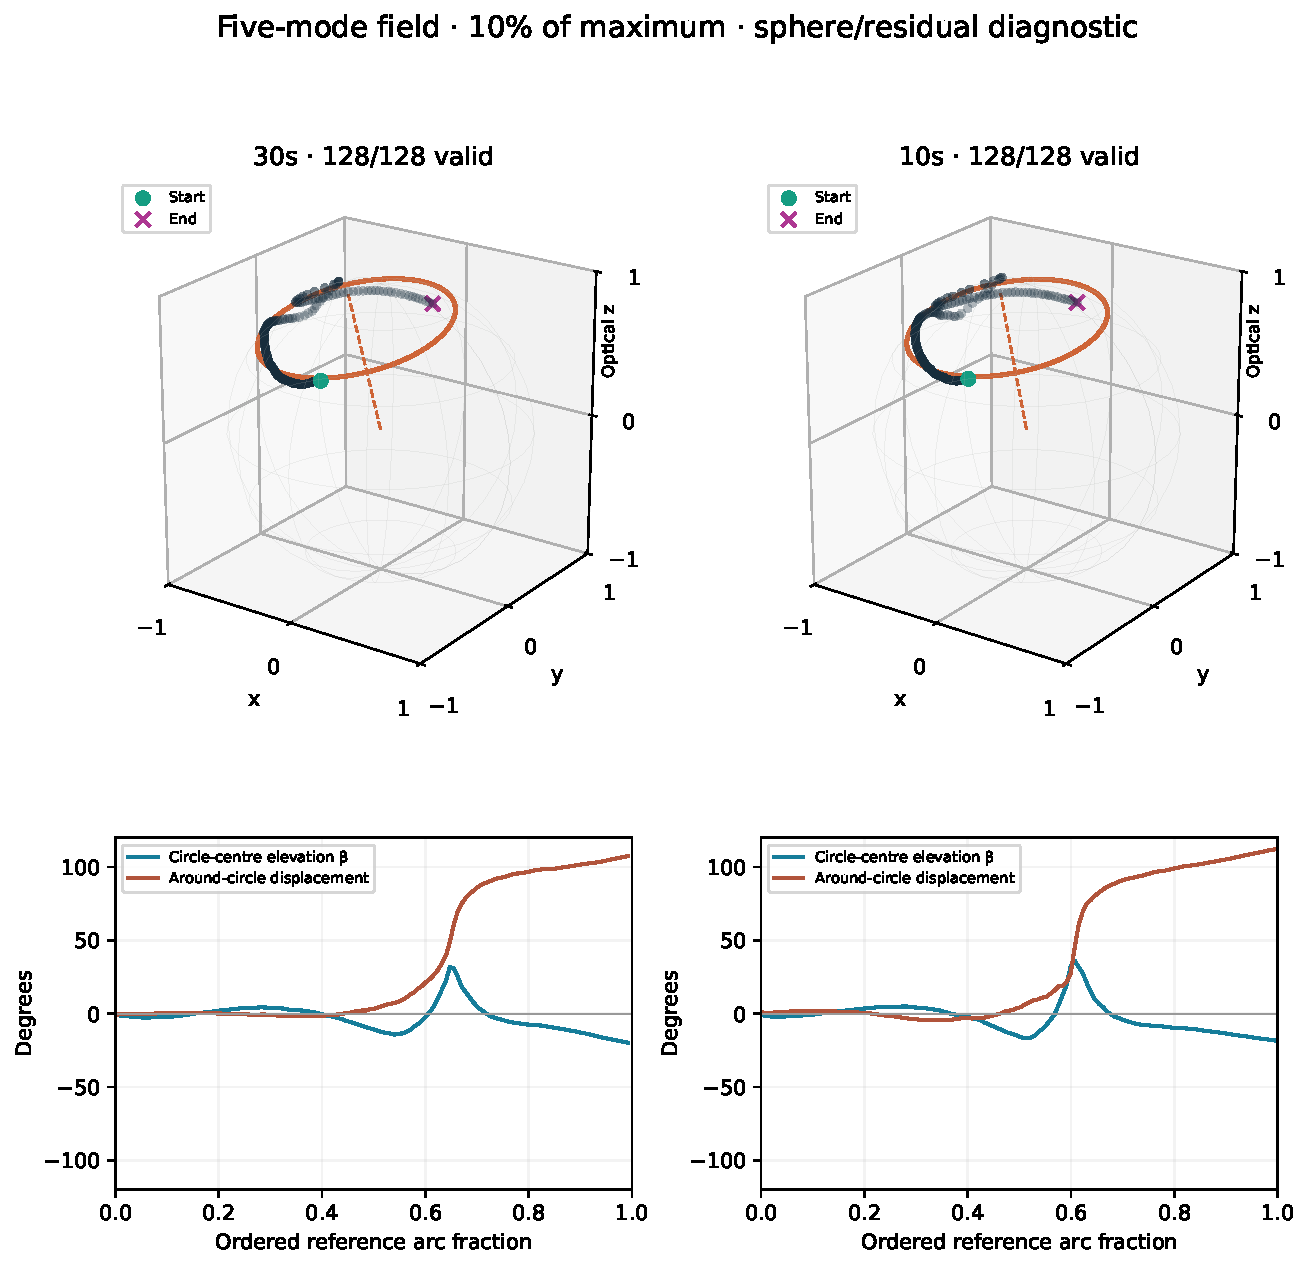
\includegraphics[width=\linewidth,height=.82\textheight,keepaspectratio]{figures/five_sphere.pdf}
30s: 128/128 valid; matched geodesic RMS 50.67$^\circ$; oriented closure mismatch 105.17$^\circ$.\par
10s: 128/128 valid; matched geodesic RMS 53.98$^\circ$; oriented closure mismatch 103.52$^\circ$.\par
\newpage
\subsection{Local cone-referenced angular residual: 10\% of maximum}\label{local:five}
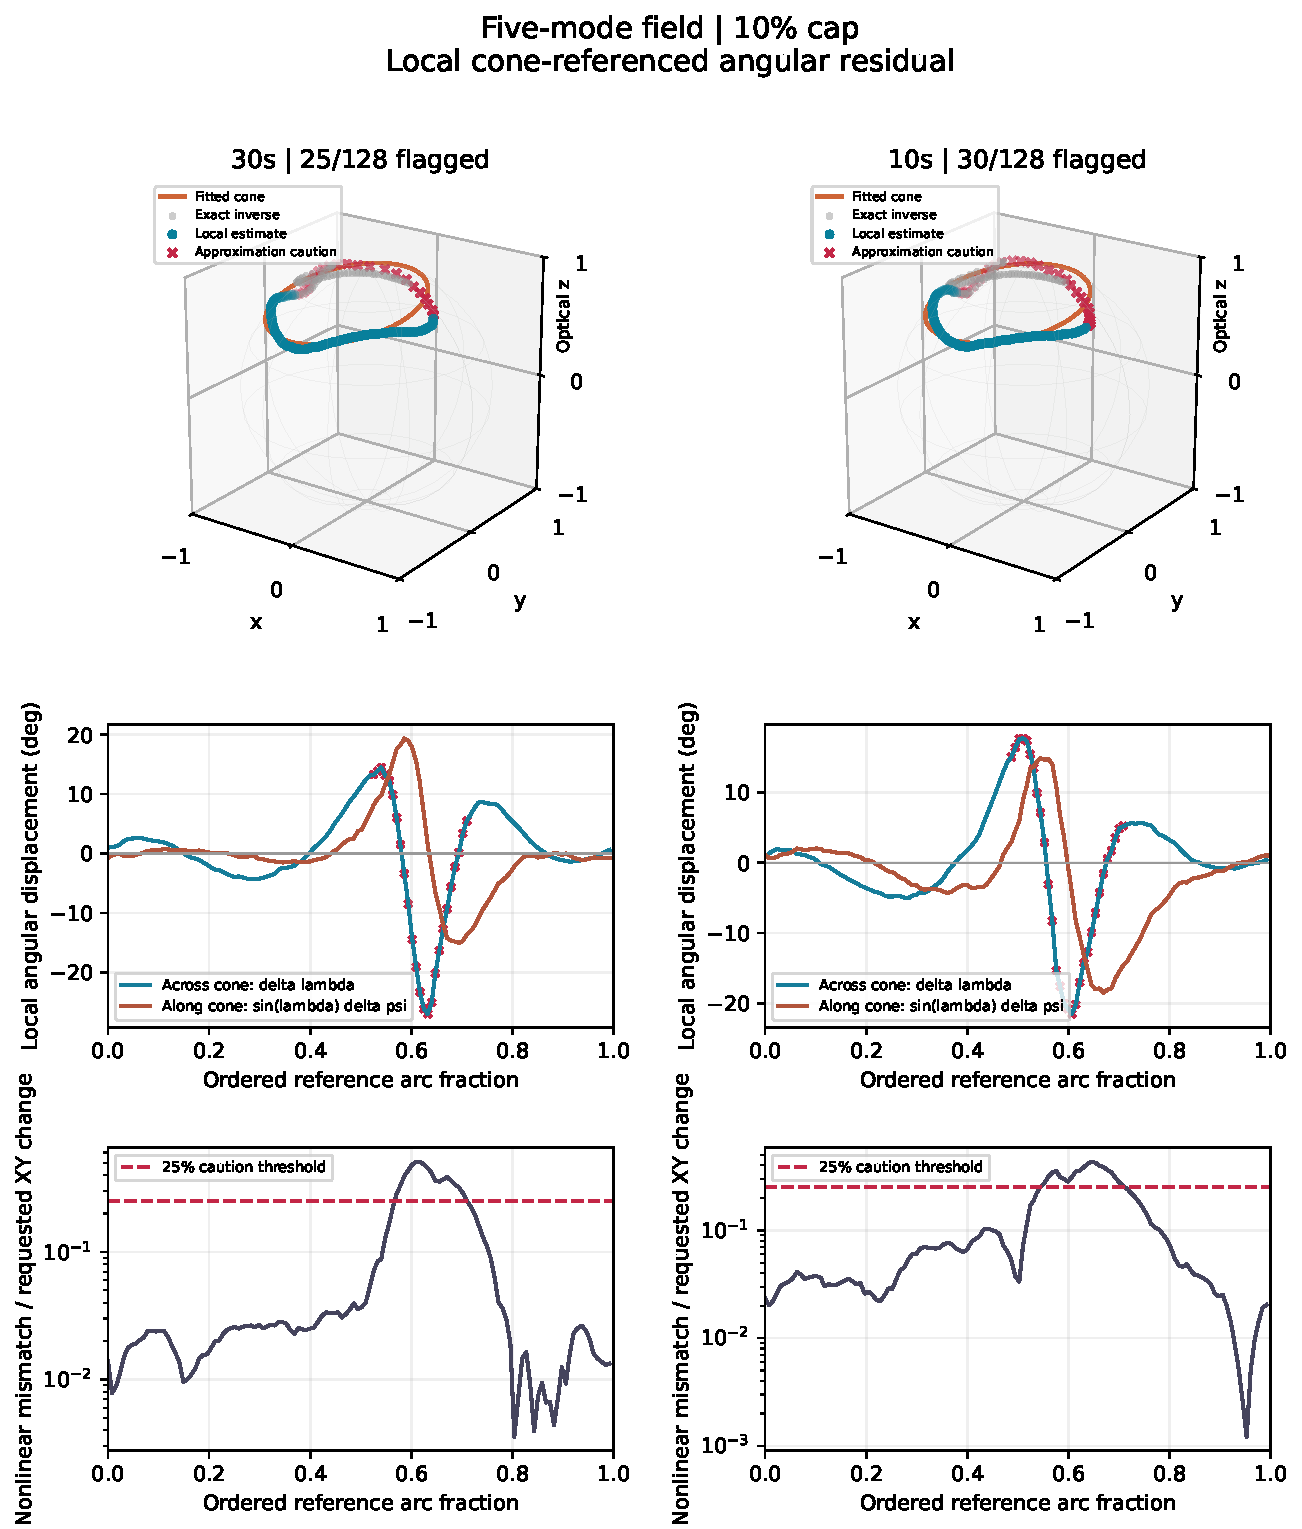
\includegraphics[width=\linewidth,height=.86\textheight,keepaspectratio]{local_residual/five.pdf}
30s: local angular RMS 9.96$^\circ$; 25/128 caution flags; median nonlinear mismatch ratio 0.025.\par
10s: local angular RMS 10.19$^\circ$; 30/128 caution flags; median nonlinear mismatch ratio 0.057.\par
\newpage
\section{General stationary field}
\[\mathbf{E}_b=\sum_{m=1}^{10}b_m\mathbf{U}_m,\qquad I_i=S_i+I_{\mathrm{int},i}+B_i.\]
Ten complex transverse pupil modes span the scalar dipole-component overlaps in this fixed-position, common-pupil model. Twenty-three shared background parameters and ten local parameters. This does not cover arbitrary moving-source fields or independent downstream analyser-path backgrounds. Uniform modes can contain a component orthogonal to this overlap span, so different basis families are not automatically identical in their background-power representation.
\textbf{Total fitted continuous parameters across both windows: 33.} The three pre-estimated gain adjustments are additional calibration parameters, held fixed here.
\begin{longtable}{llrrrrrr}\toprule
Budget & Window & BG\% & Meas.RMS & Signal RMS & Bad(train/test) & Max $r$ & Conv.\\\midrule\endhead
uncapped & 30s & 52.8 & 0.0049 & 0.0324 & 12/16 & 1.491 & yes \\
uncapped & 10s & 52.6 & 0.0097 & 0.0468 & 0/19 & 1.647 & yes \\
5pct & 30s & 5.0 & 0.0196 & 0.0227 & 0/0 & 0.593 & yes \\
5pct & 10s & 5.0 & 0.0231 & 0.0261 & 0/0 & 0.602 & yes \\
10pct & 30s & 10.0 & 0.0114 & 0.0139 & 0/0 & 0.658 & yes \\
10pct & 10s & 10.0 & 0.0144 & 0.0175 & 0/0 & 0.608 & yes \\
20pct & 30s & 20.0 & 0.0070 & 0.0083 & 0/0 & 0.733 & yes \\
20pct & 10s & 19.9 & 0.0102 & 0.0130 & 0/0 & 0.701 & yes \\
30pct & 30s & 30.0 & 0.0063 & 0.0080 & 0/0 & 0.768 & yes \\
30pct & 10s & 29.9 & 0.0098 & 0.0129 & 0/0 & 0.733 & yes \\
40pct & 30s & 40.0 & 0.0059 & 0.0090 & 0/0 & 0.783 & yes \\
40pct & 10s & 39.8 & 0.0097 & 0.0143 & 0/0 & 0.735 & yes \\
50pct & 30s & 50.0 & 0.0052 & 0.0275 & 12/16 & 0.945 & yes \\
50pct & 10s & 49.8 & 0.0098 & 0.0403 & 0/19 & 1.219 & yes \\
\bottomrule\end{longtable}
\begin{longtable}{llrrrr}\toprule
Budget & Window & Signal\% range & Cross\% range & Noninterf.BG\% & Fitted folded $\theta$\\\midrule\endhead
uncapped & 30s & 2.1--110.3 & -78.2--5.9 & 0.0 & 8.3--89.9$^\circ$ \\
uncapped & 10s & 4.4--101.5 & -71.9--6.9 & 0.0 & 12.7--89.7$^\circ$ \\
5pct & 30s & 45.9--99.5 & -15.6--14.8 & 0.0 & 31.9--49.9$^\circ$ \\
5pct & 10s & 51.7--95.3 & -15.3--15.0 & 0.0 & 34.0--48.5$^\circ$ \\
10pct & 30s & 42.2--91.9 & -11.9--17.7 & 0.0 & 34.6--55.1$^\circ$ \\
10pct & 10s & 47.3--88.7 & -11.7--17.9 & 0.0 & 36.6--53.4$^\circ$ \\
20pct & 30s & 40.9--94.0 & -27.2--23.2 & 0.0 & 35.8--60.2$^\circ$ \\
20pct & 10s & 42.2--93.7 & -27.9--23.2 & 0.0 & 35.9--58.8$^\circ$ \\
30pct & 30s & 38.5--99.3 & -38.4--16.3 & 6.5 & 34.7--62.8$^\circ$ \\
30pct & 10s & 39.6--98.8 & -40.0--16.5 & 6.4 & 34.5--60.8$^\circ$ \\
40pct & 30s & 28.3--104.3 & -55.4--6.7 & 8.7 & 29.1--64.7$^\circ$ \\
40pct & 10s & 34.4--99.3 & -52.4--6.4 & 8.7 & 32.3--61.9$^\circ$ \\
50pct & 30s & 3.2--107.4 & -72.6--8.0 & 0.0 & 10.5--89.8$^\circ$ \\
50pct & 10s & 5.9--98.7 & -66.7--9.0 & 0.0 & 14.9--89.7$^\circ$ \\
\bottomrule\end{longtable}
\textbf{Per-channel constant background, percent of measured maximum:}
\begin{longtable}{llrrrr}\toprule
Budget & Window & $B_0$ & $B_{90}$ & $B_{45}$ & $B_{135}$\\\midrule\endhead
uncapped & 30s & 16.46 & 9.95 & 11.06 & 15.35\\
uncapped & 10s & 16.38 & 9.90 & 11.01 & 15.28\\
5pct & 30s & 1.94 & 0.56 & 0.66 & 1.84\\
5pct & 10s & 1.93 & 0.56 & 0.66 & 1.83\\
10pct & 30s & 4.19 & 0.81 & 1.35 & 3.65\\
10pct & 10s & 4.17 & 0.80 & 1.34 & 3.64\\
20pct & 30s & 9.19 & 0.81 & 3.24 & 6.76\\
20pct & 10s & 9.15 & 0.81 & 3.22 & 6.73\\
30pct & 30s & 13.86 & 1.14 & 5.10 & 9.90\\
30pct & 10s & 13.80 & 1.14 & 5.07 & 9.86\\
40pct & 30s & 16.03 & 3.97 & 6.38 & 13.62\\
40pct & 10s & 15.96 & 3.95 & 6.35 & 13.55\\
50pct & 30s & 16.10 & 8.90 & 10.27 & 14.73\\
50pct & 10s & 16.02 & 8.86 & 10.22 & 14.66\\
\bottomrule\end{longtable}
\newpage
\subsection{No BG-power cap}\label{case:general:uncapped}
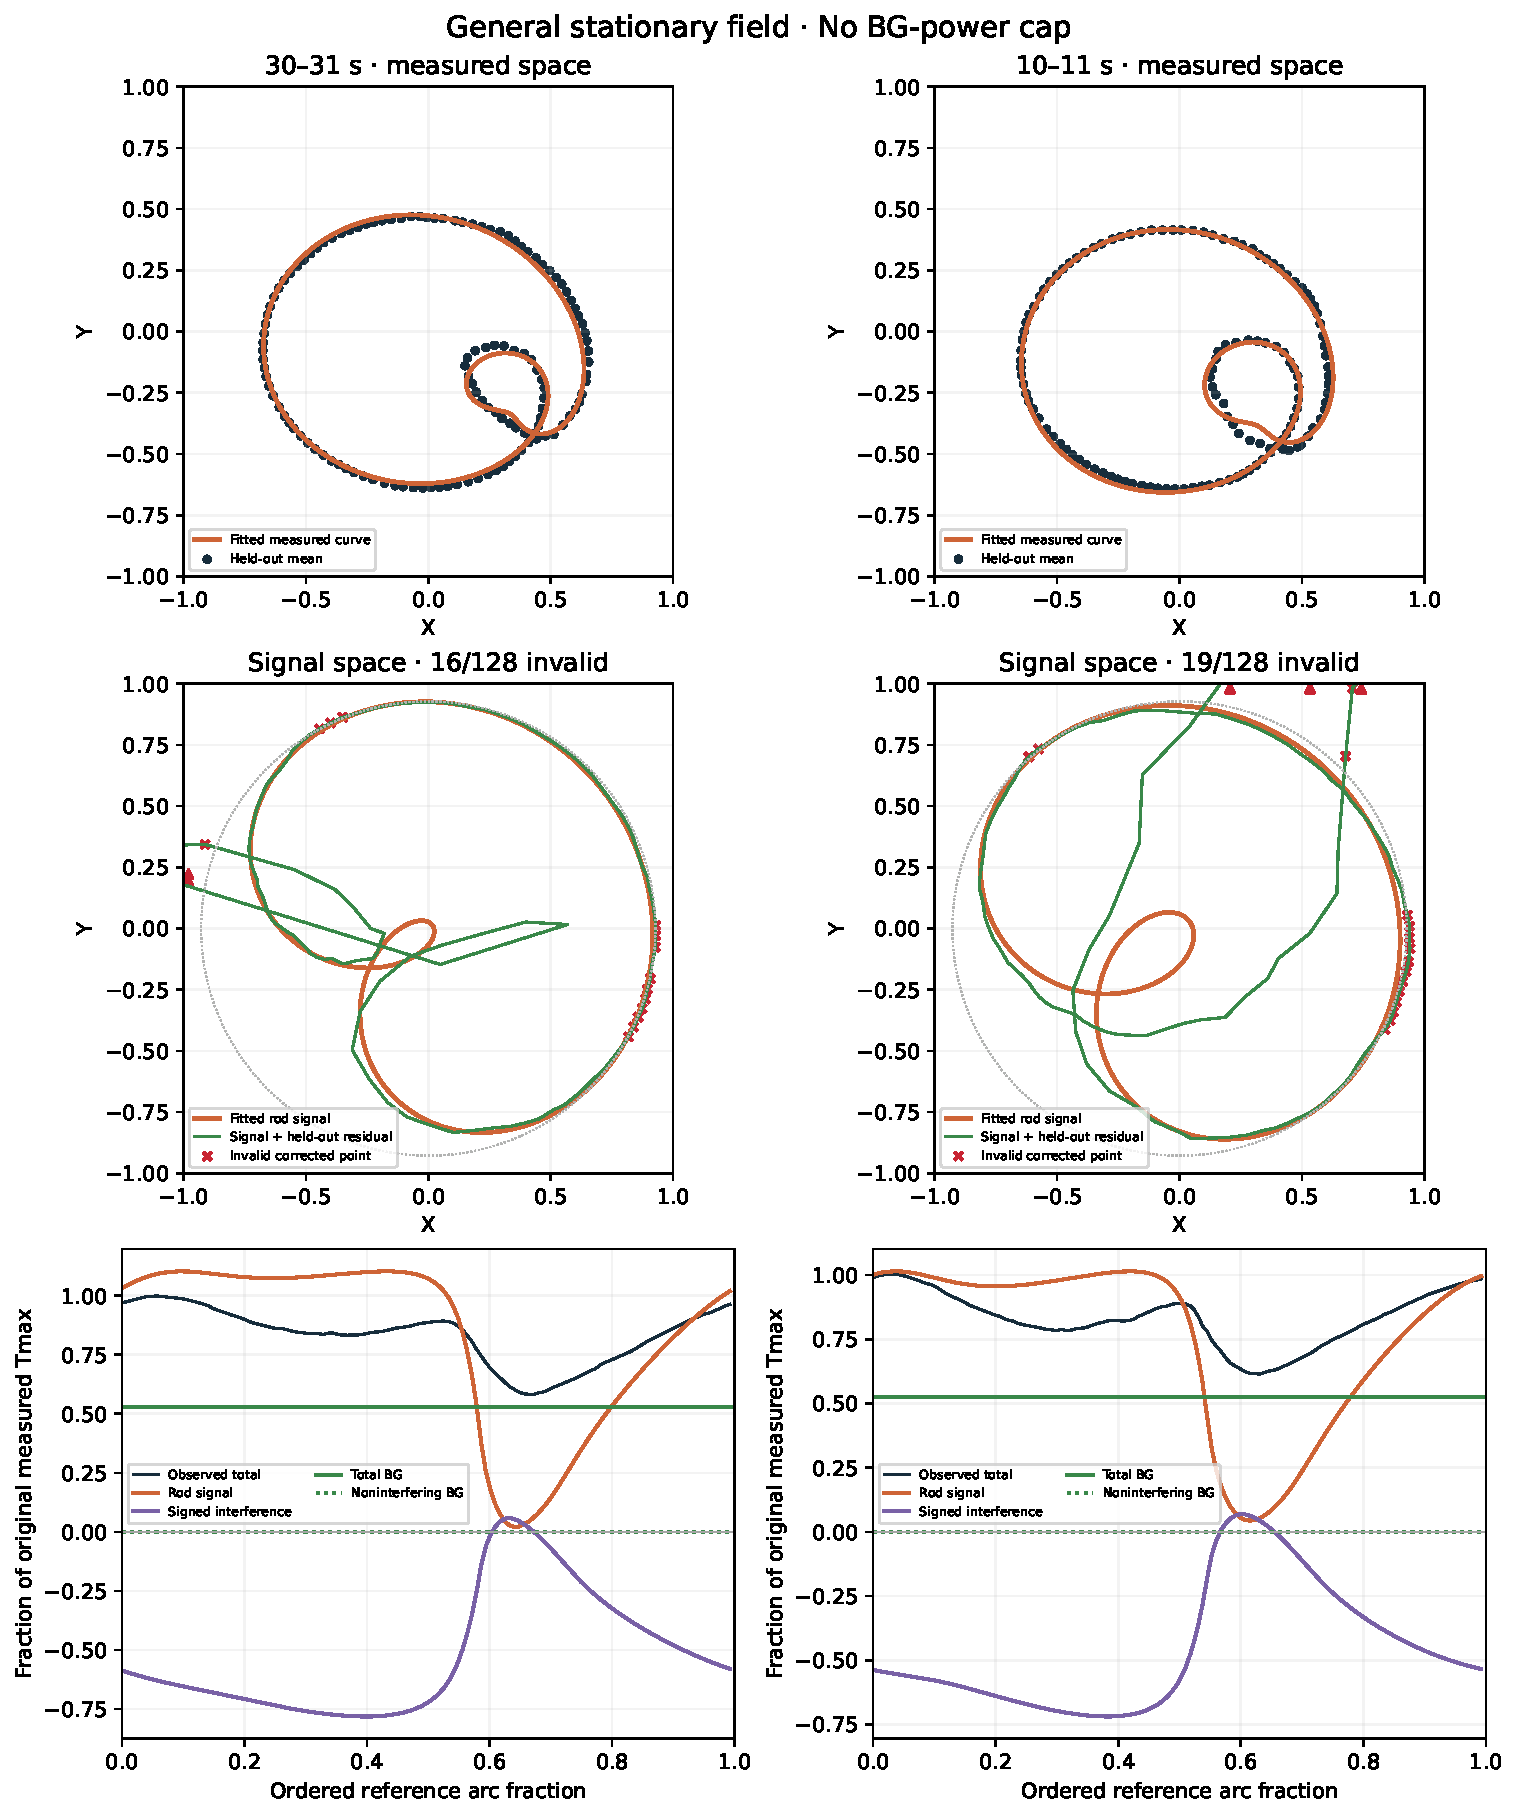
\includegraphics[width=\linewidth,height=.9\textheight,keepaspectratio]{figures/general_uncapped.pdf}
\newpage
\subsection{5\% of maximum}\label{case:general:5pct}
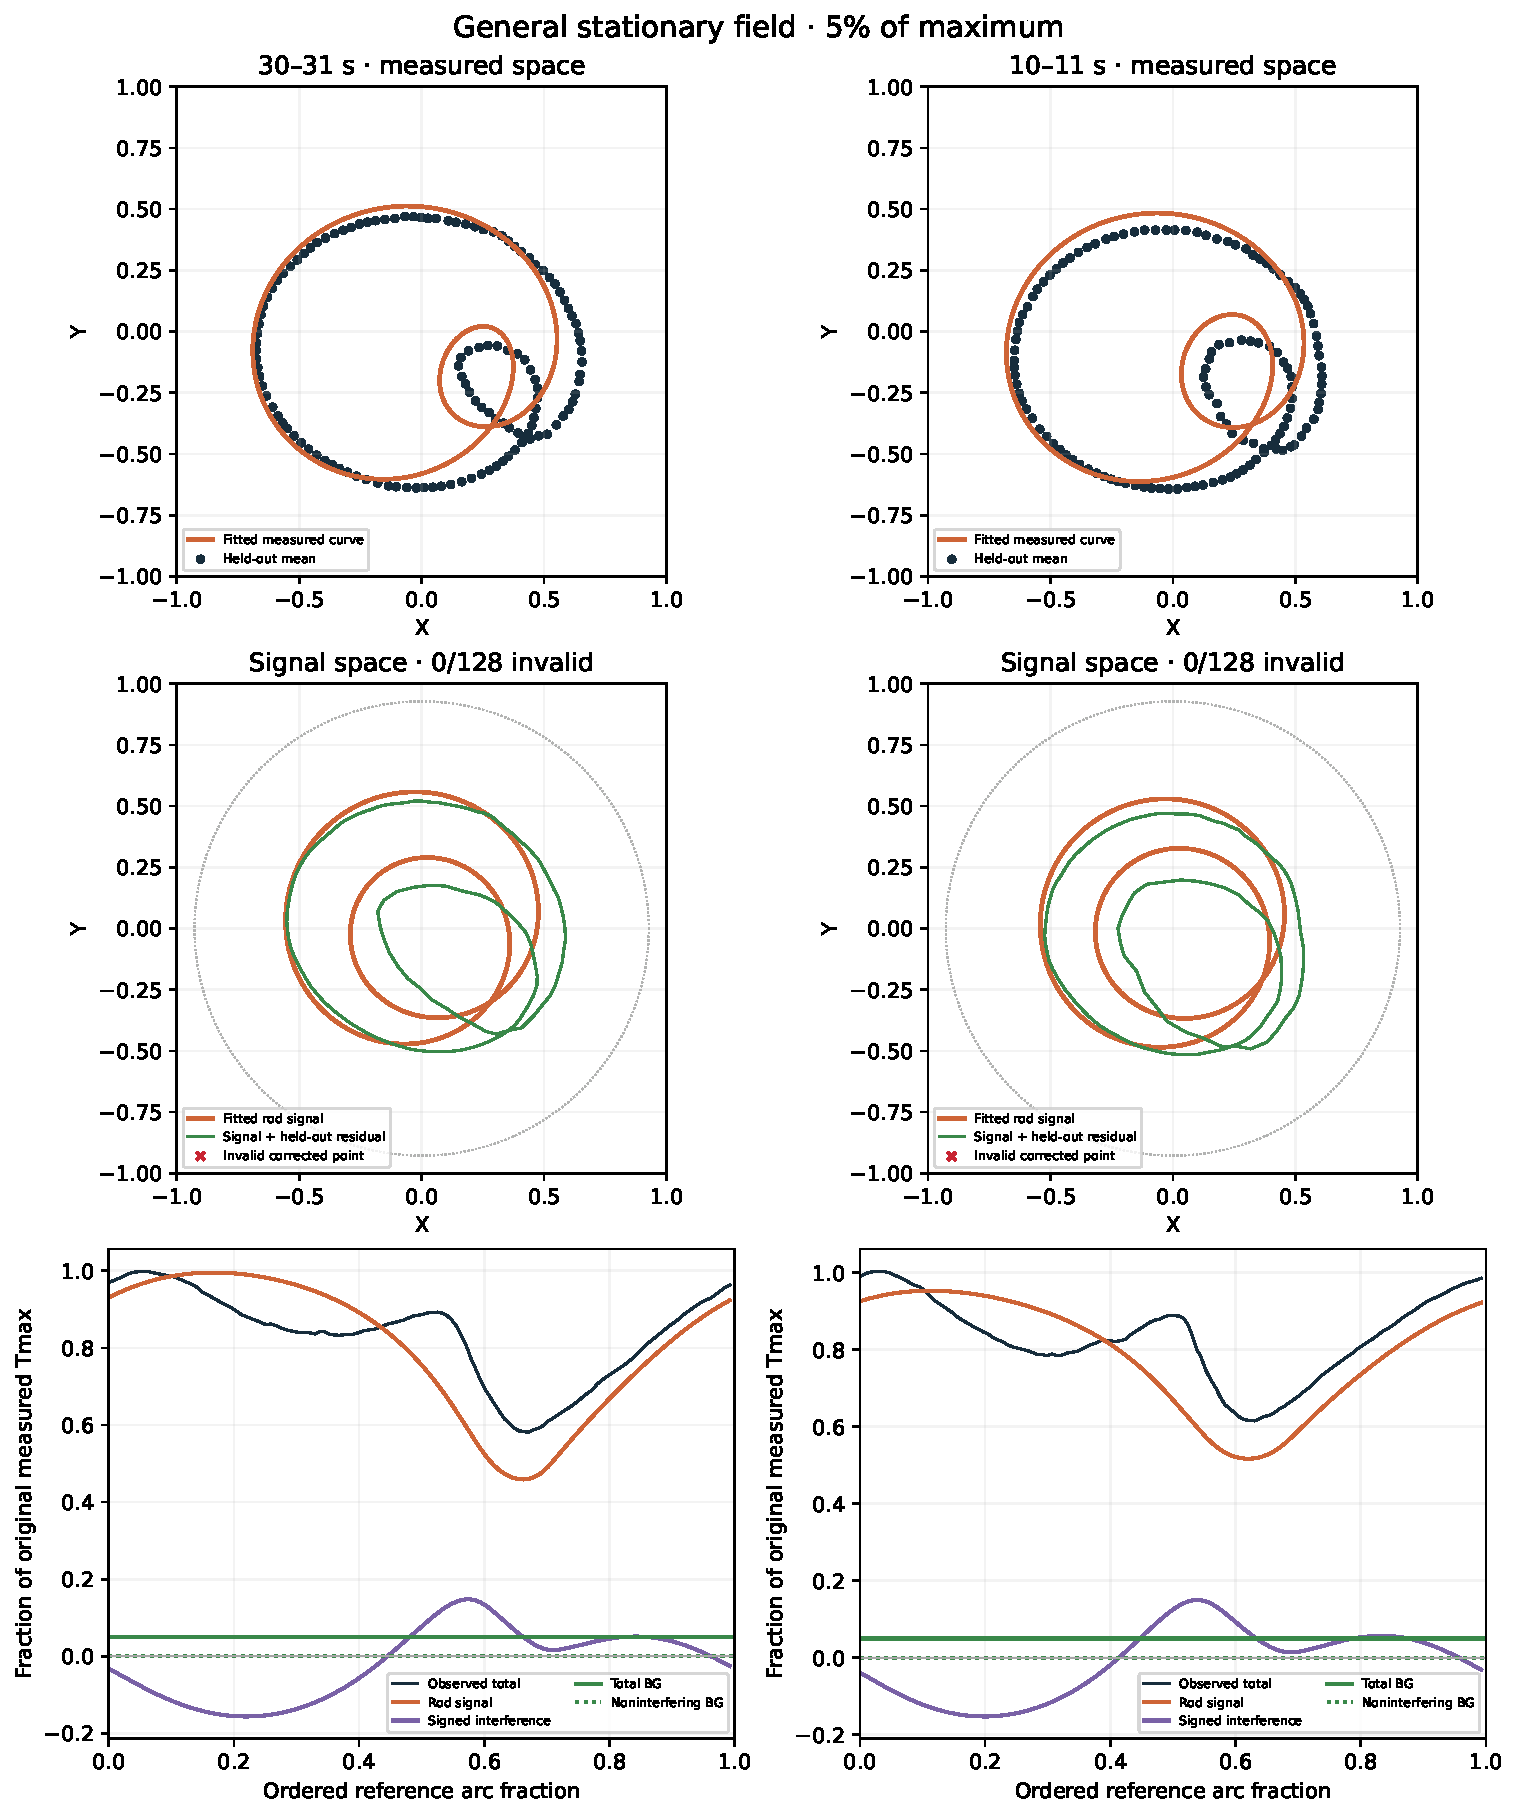
\includegraphics[width=\linewidth,height=.9\textheight,keepaspectratio]{figures/general_5pct.pdf}
\newpage
\subsection{10\% of maximum}\label{case:general:10pct}
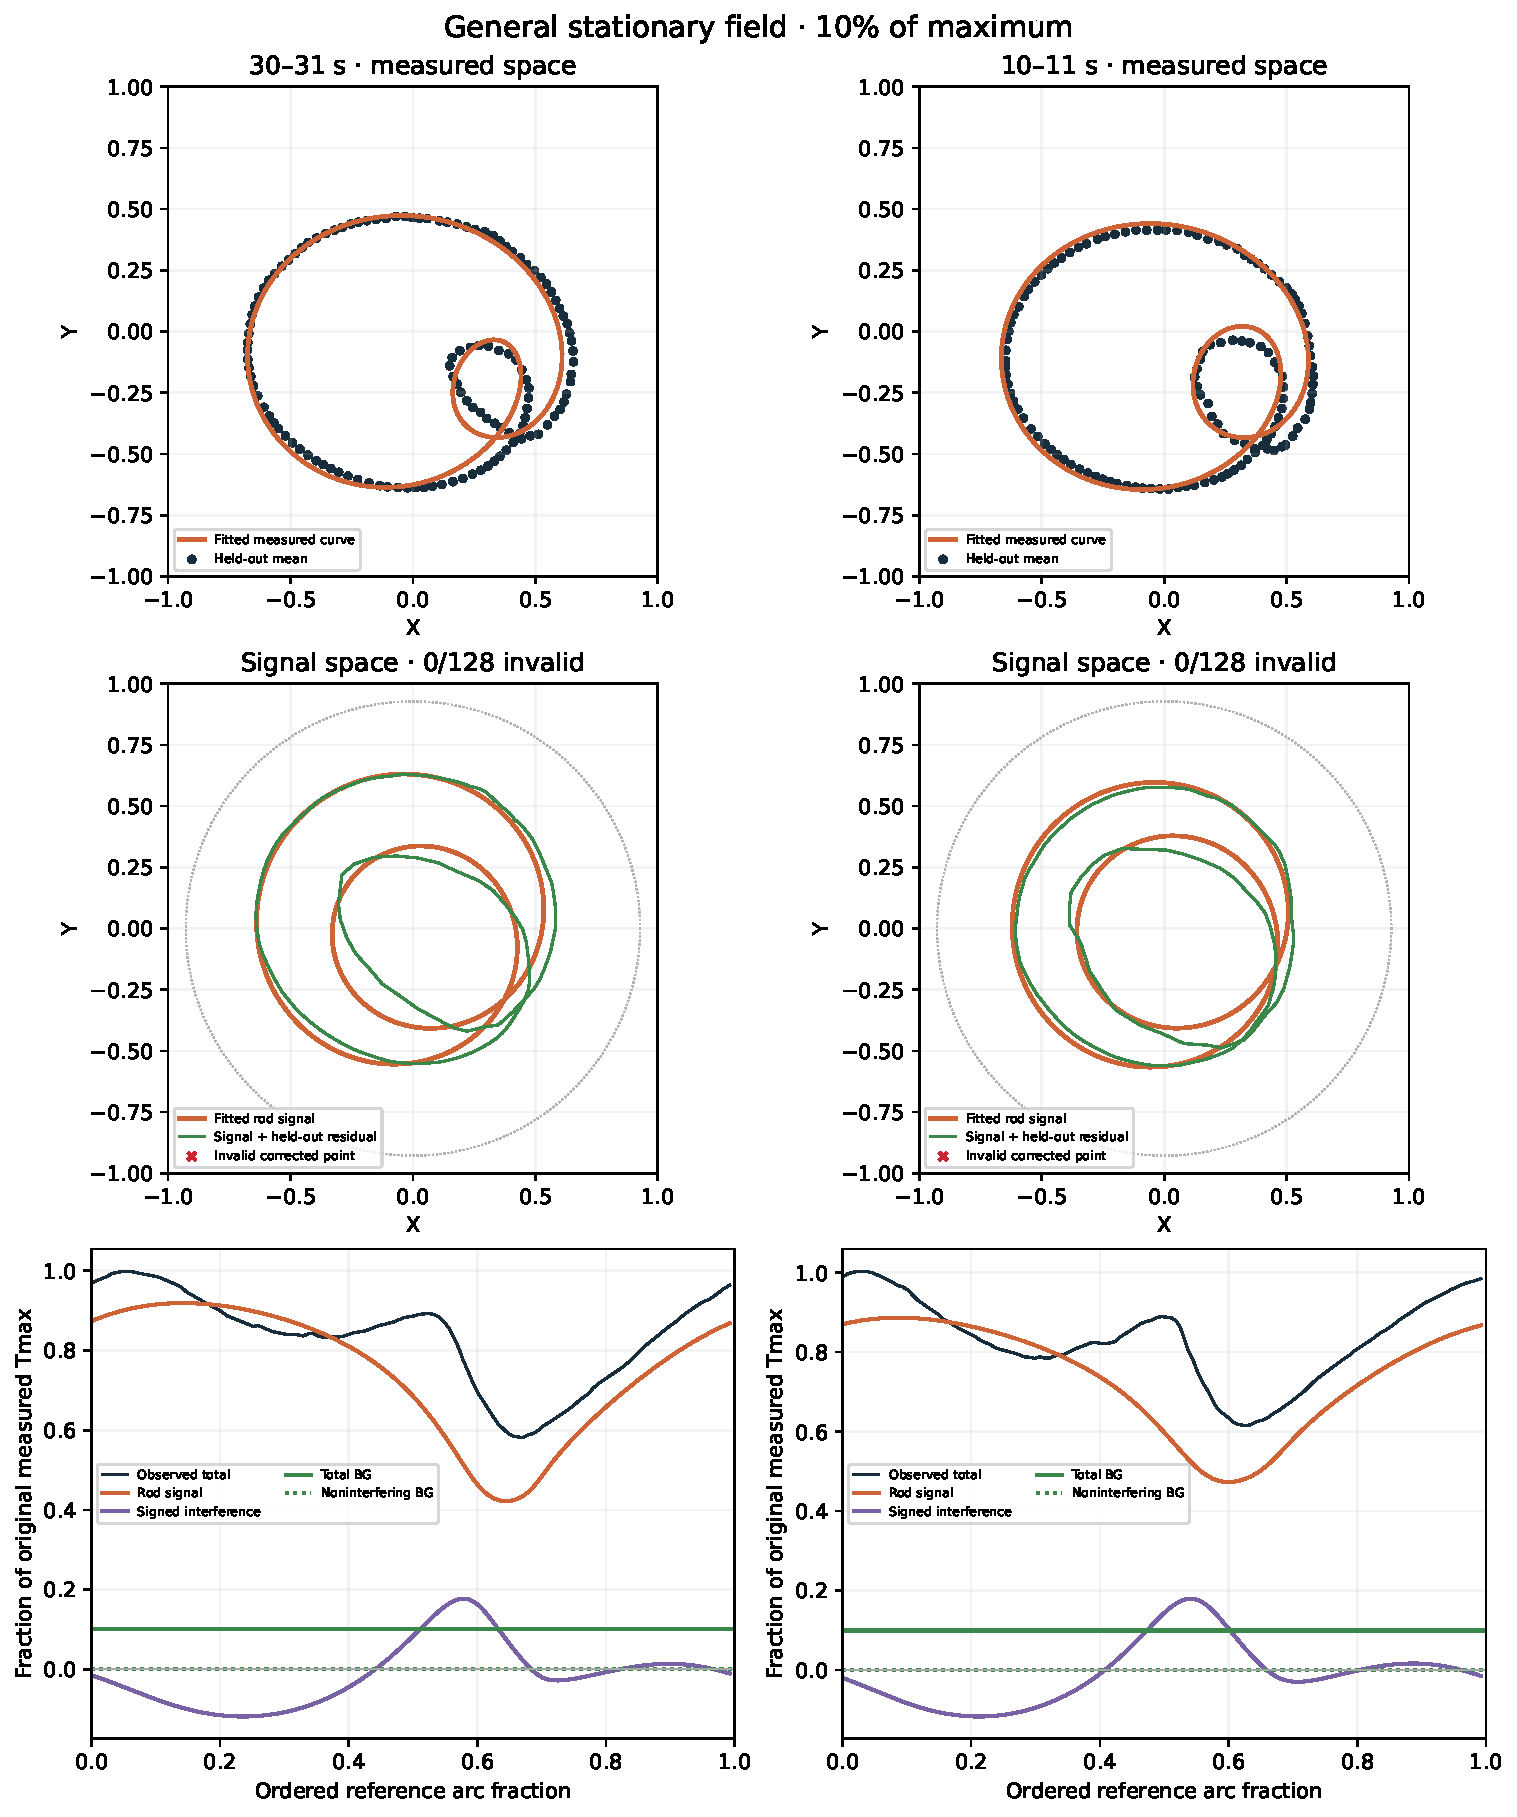
\includegraphics[width=\linewidth,height=.9\textheight,keepaspectratio]{figures/general_10pct.pdf}
\newpage
\subsection{20\% of maximum}\label{case:general:20pct}
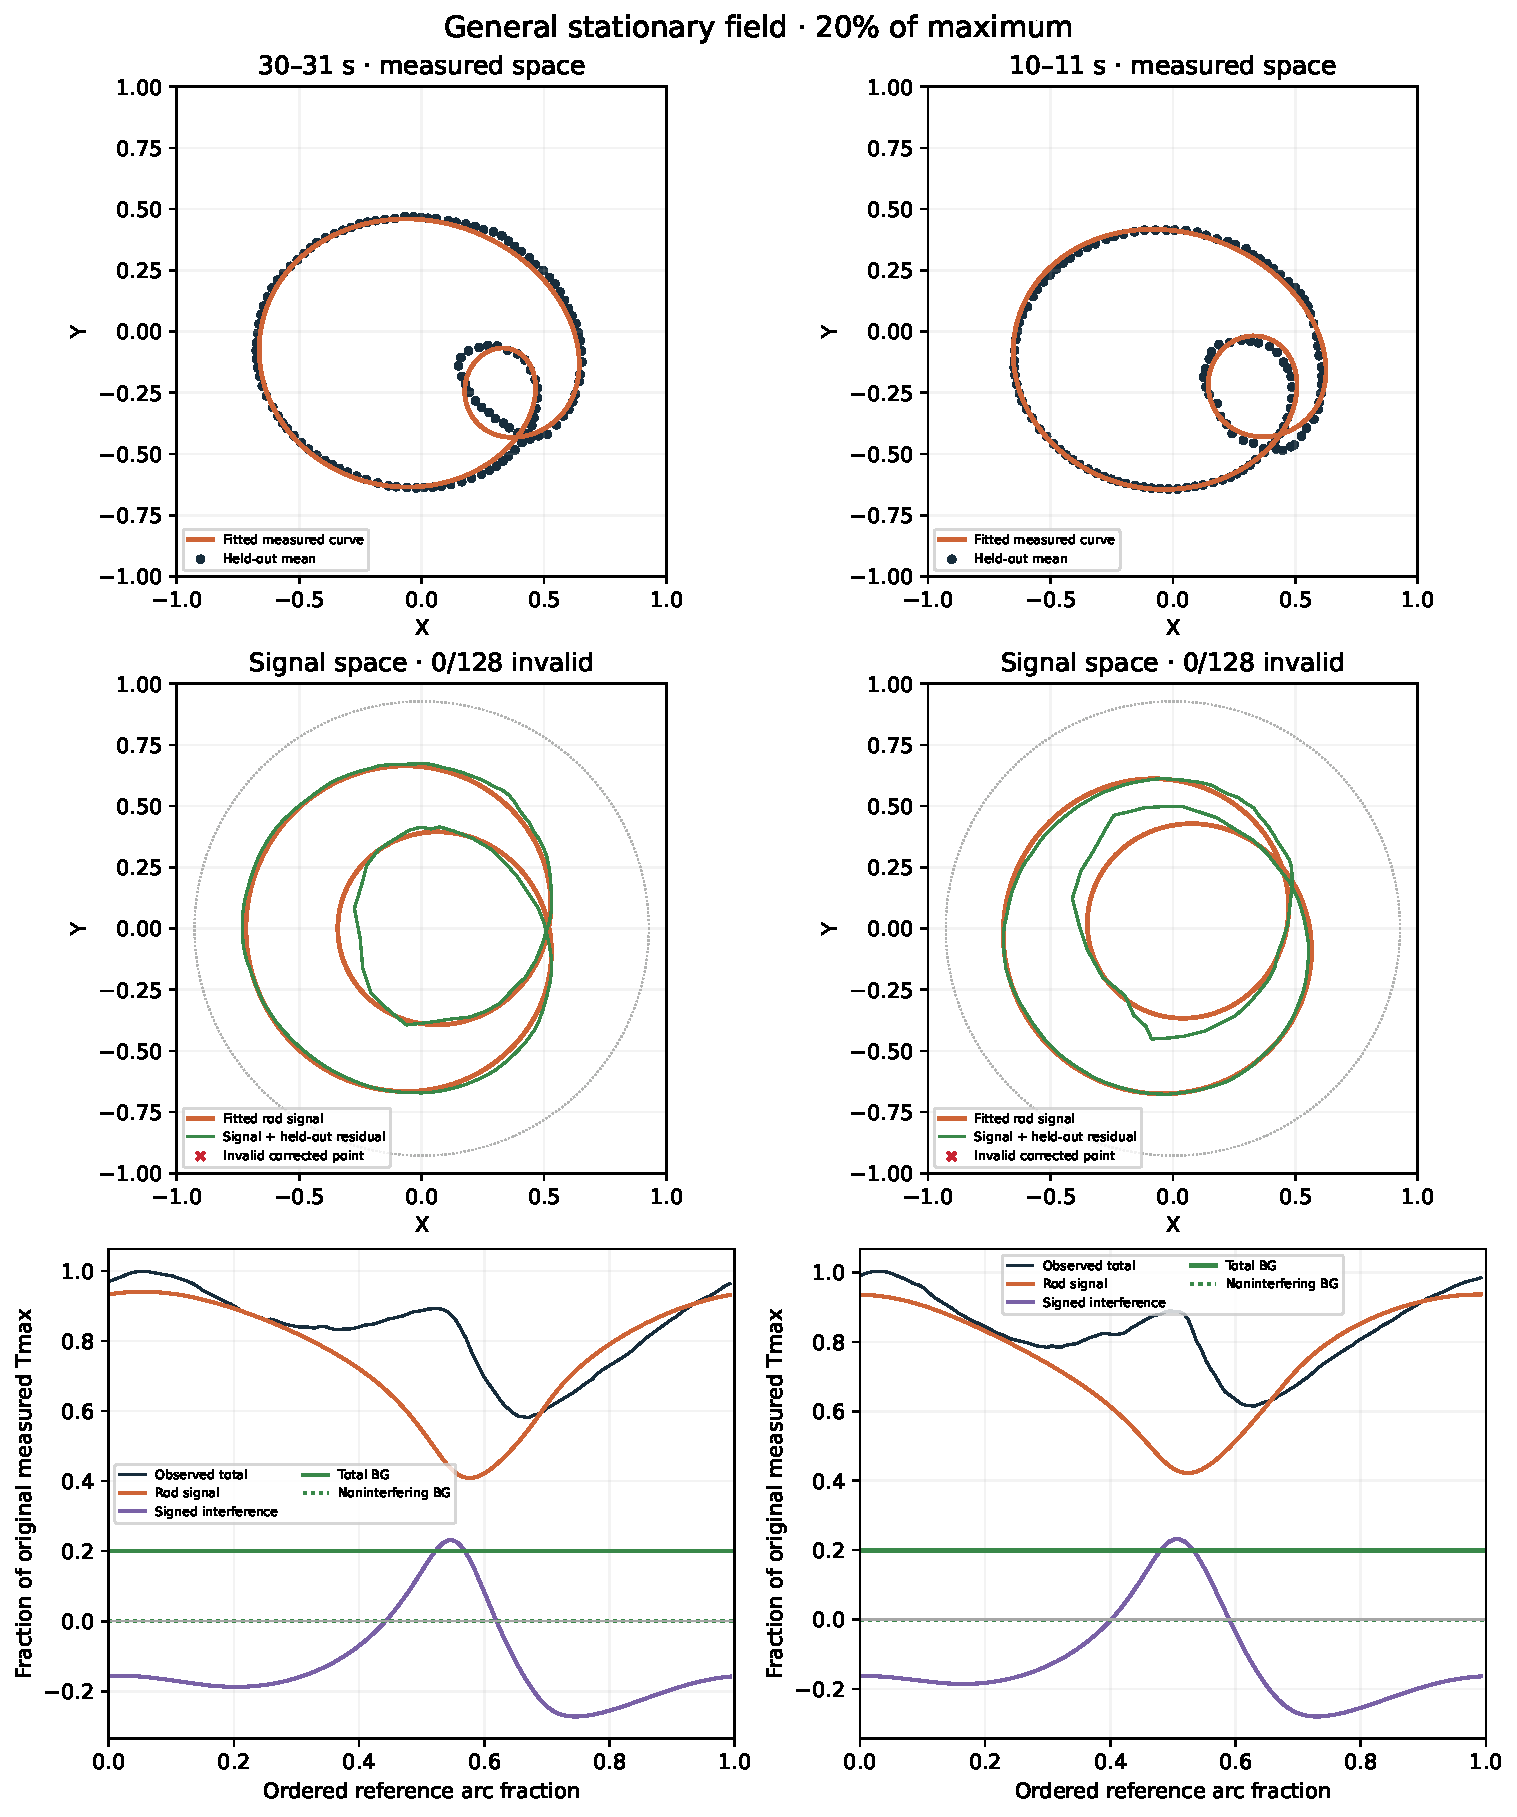
\includegraphics[width=\linewidth,height=.9\textheight,keepaspectratio]{figures/general_20pct.pdf}
\newpage
\subsection{30\% of maximum}\label{case:general:30pct}
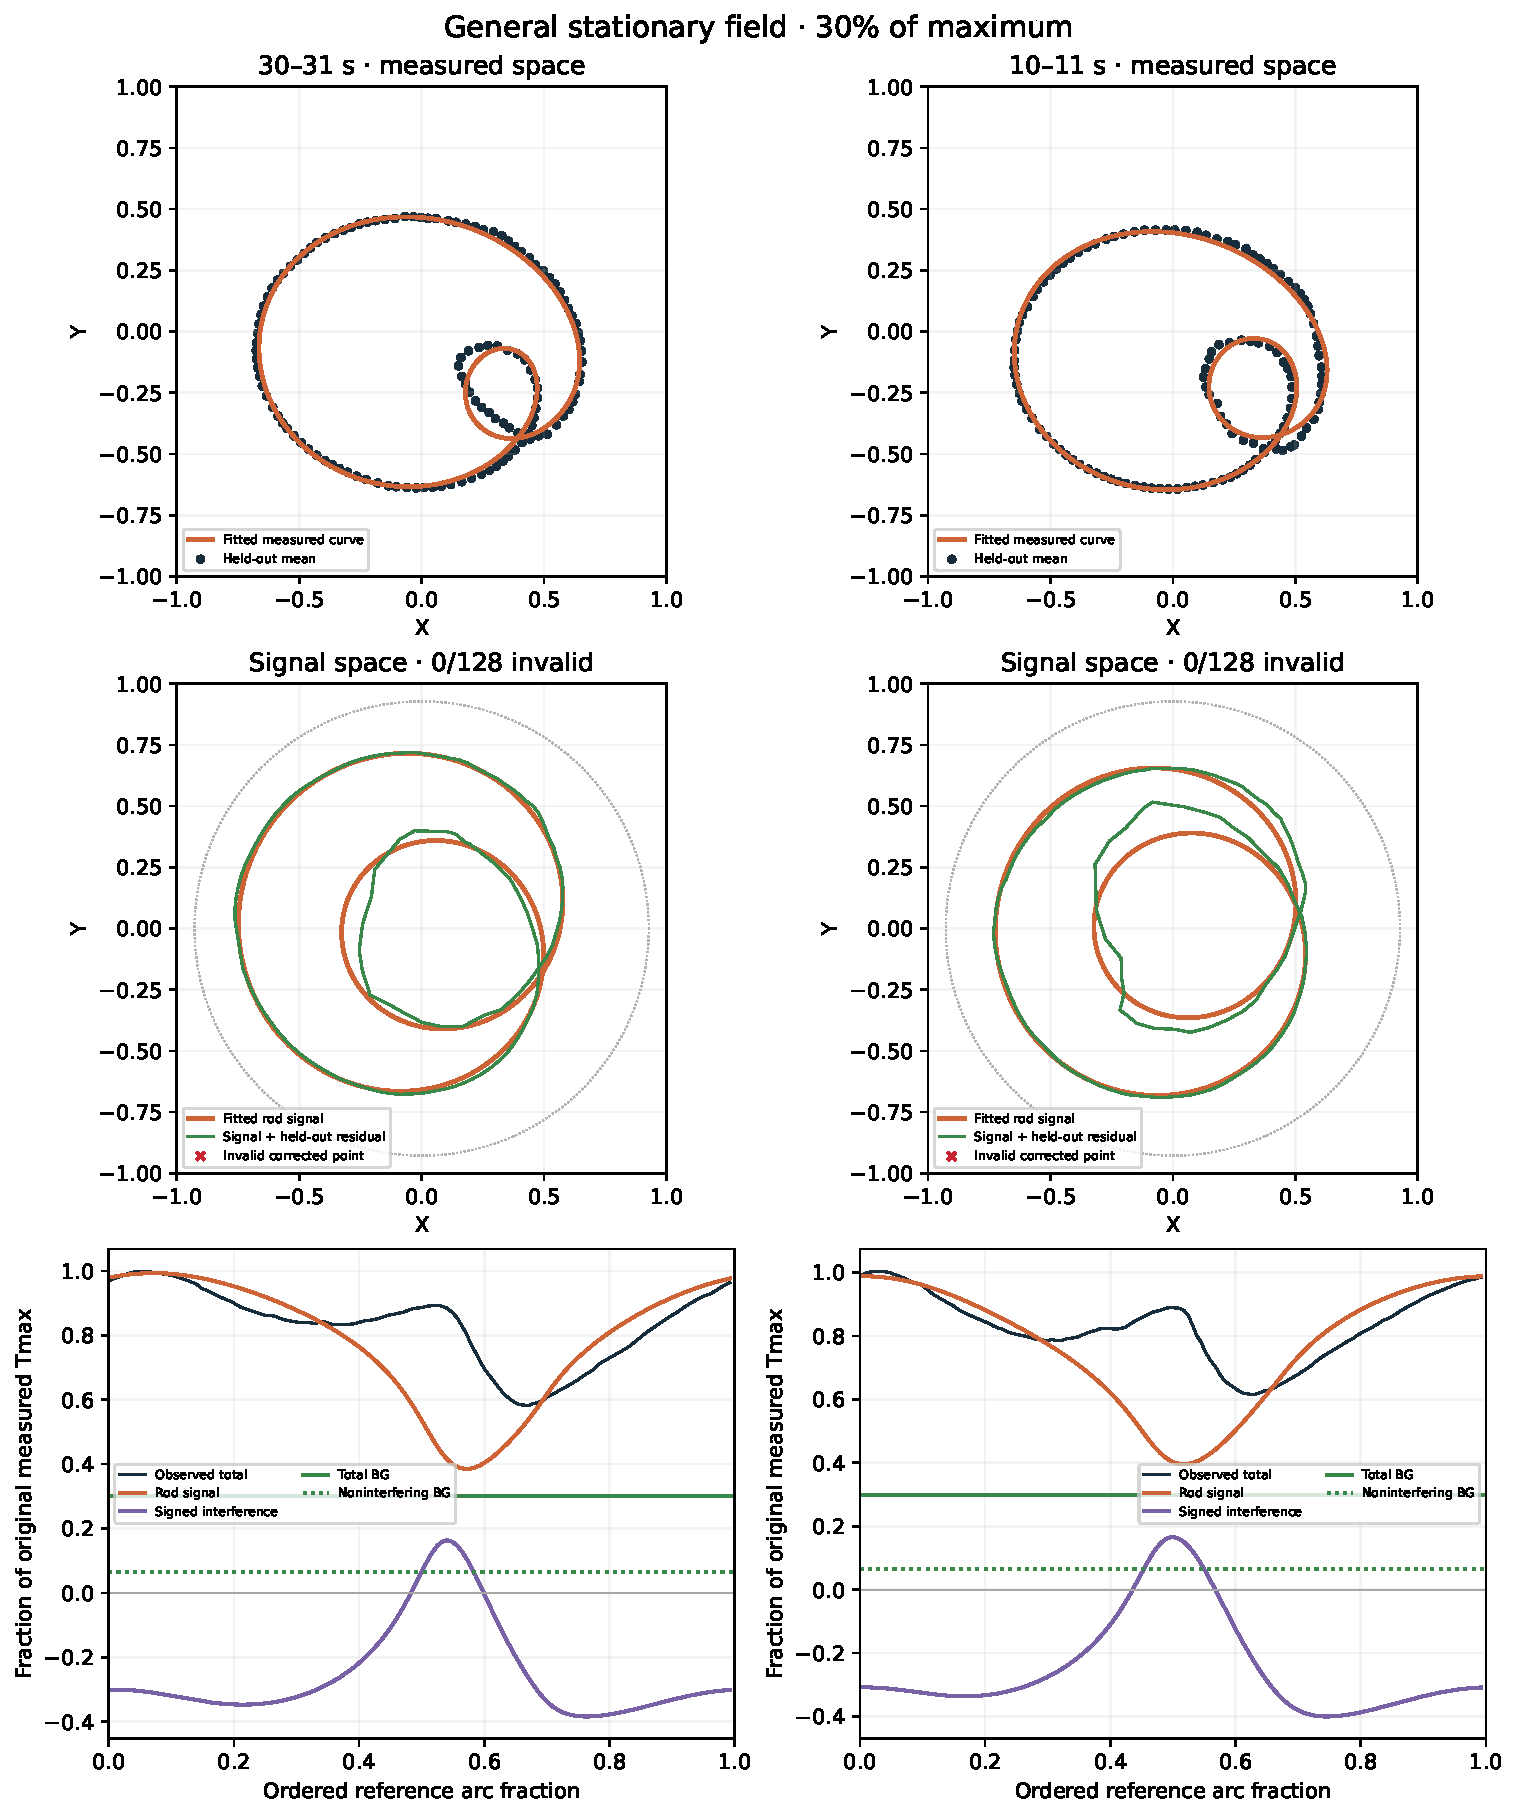
\includegraphics[width=\linewidth,height=.9\textheight,keepaspectratio]{figures/general_30pct.pdf}
\newpage
\subsection{40\% of maximum}\label{case:general:40pct}
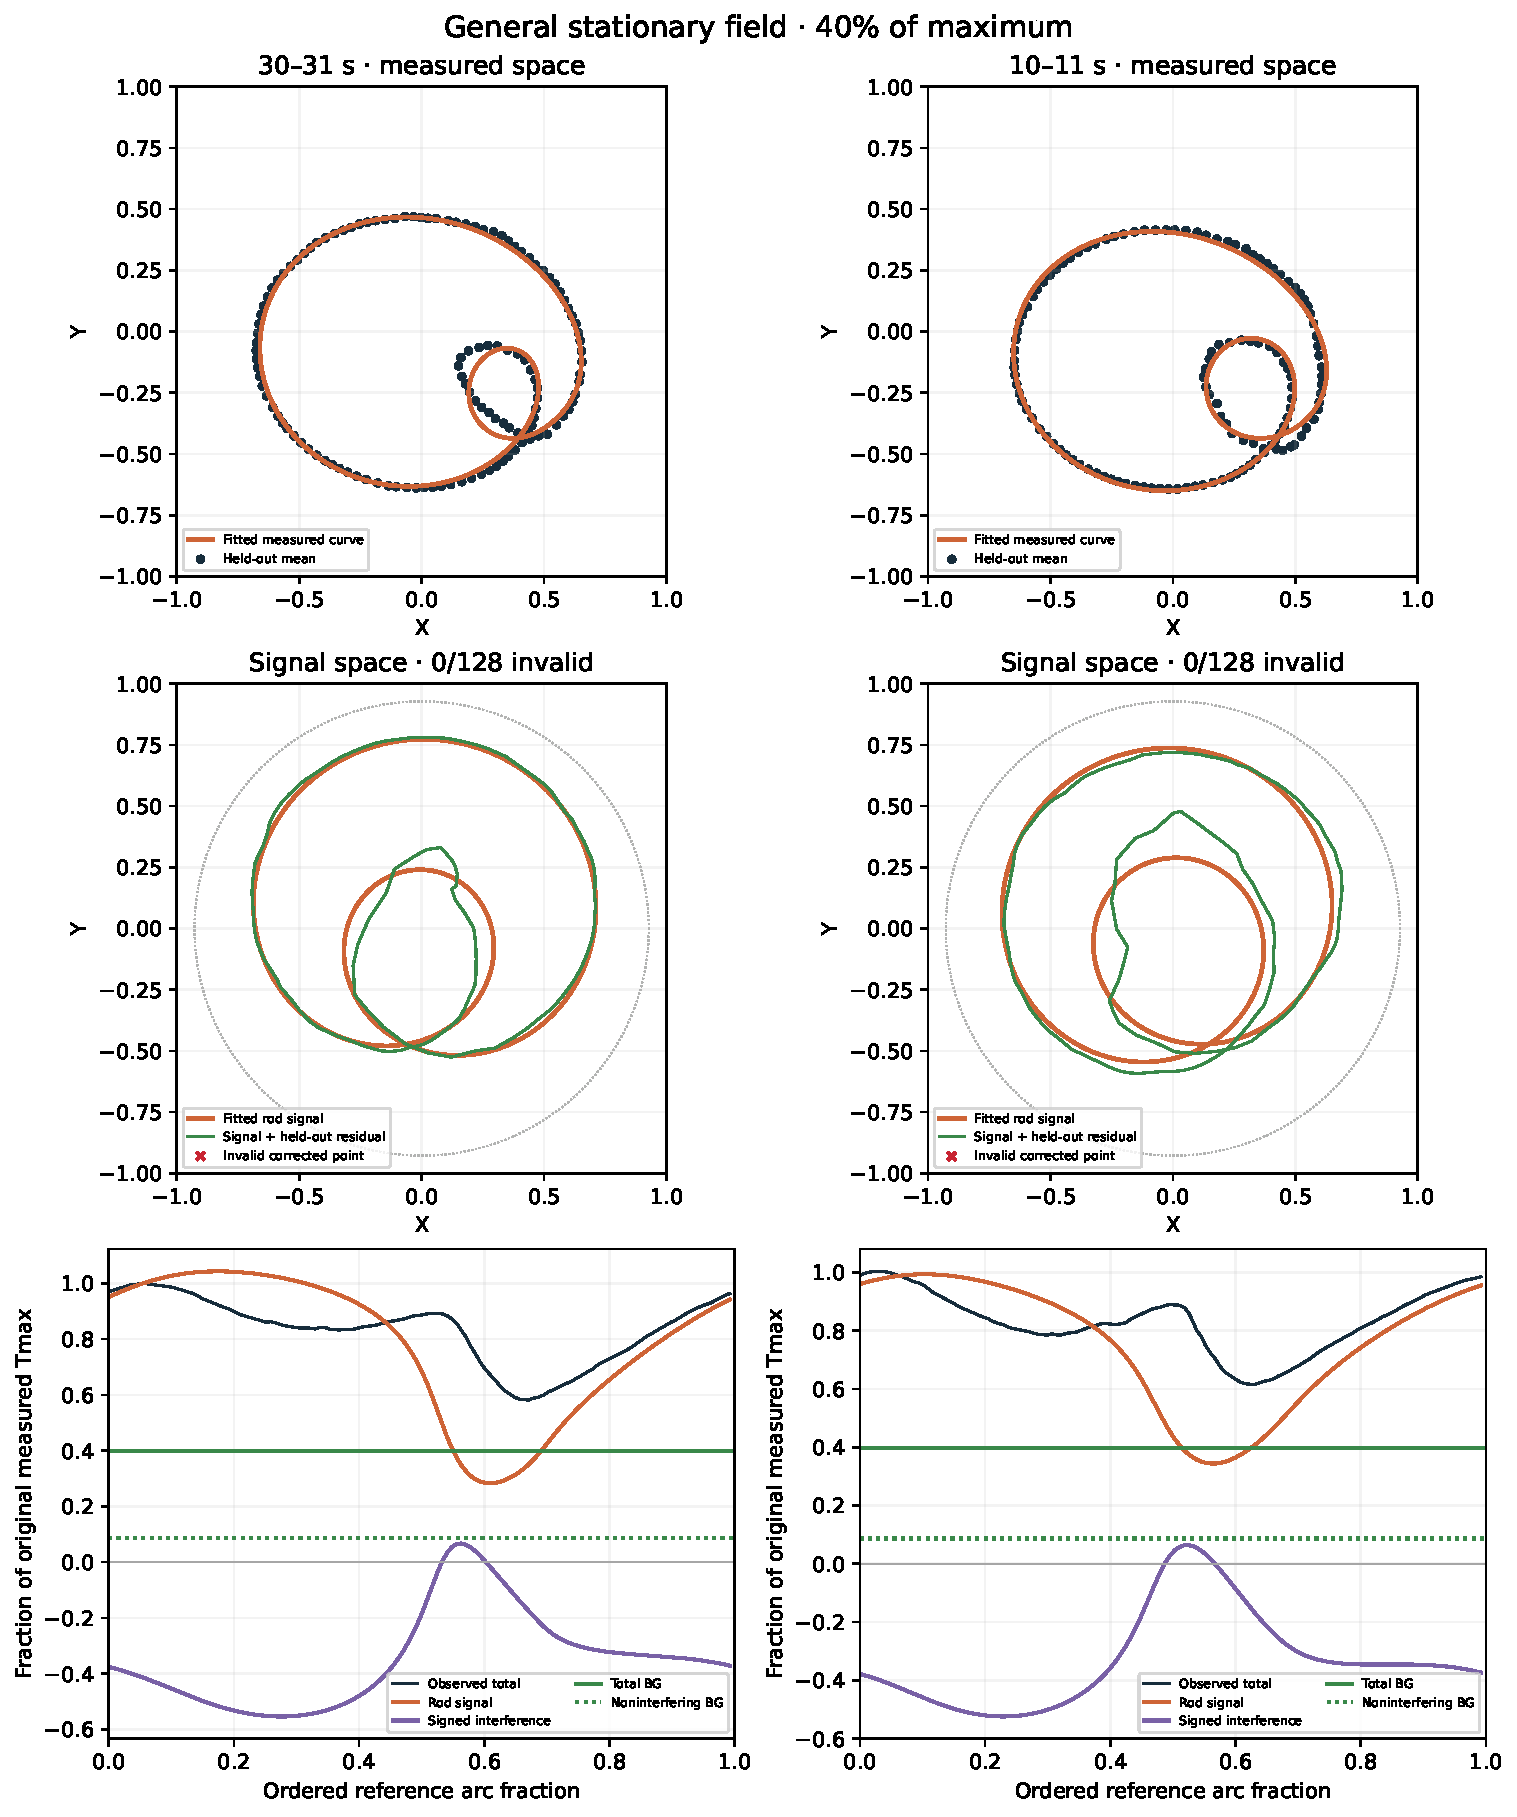
\includegraphics[width=\linewidth,height=.9\textheight,keepaspectratio]{figures/general_40pct.pdf}
\newpage
\subsection{50\% of maximum}\label{case:general:50pct}
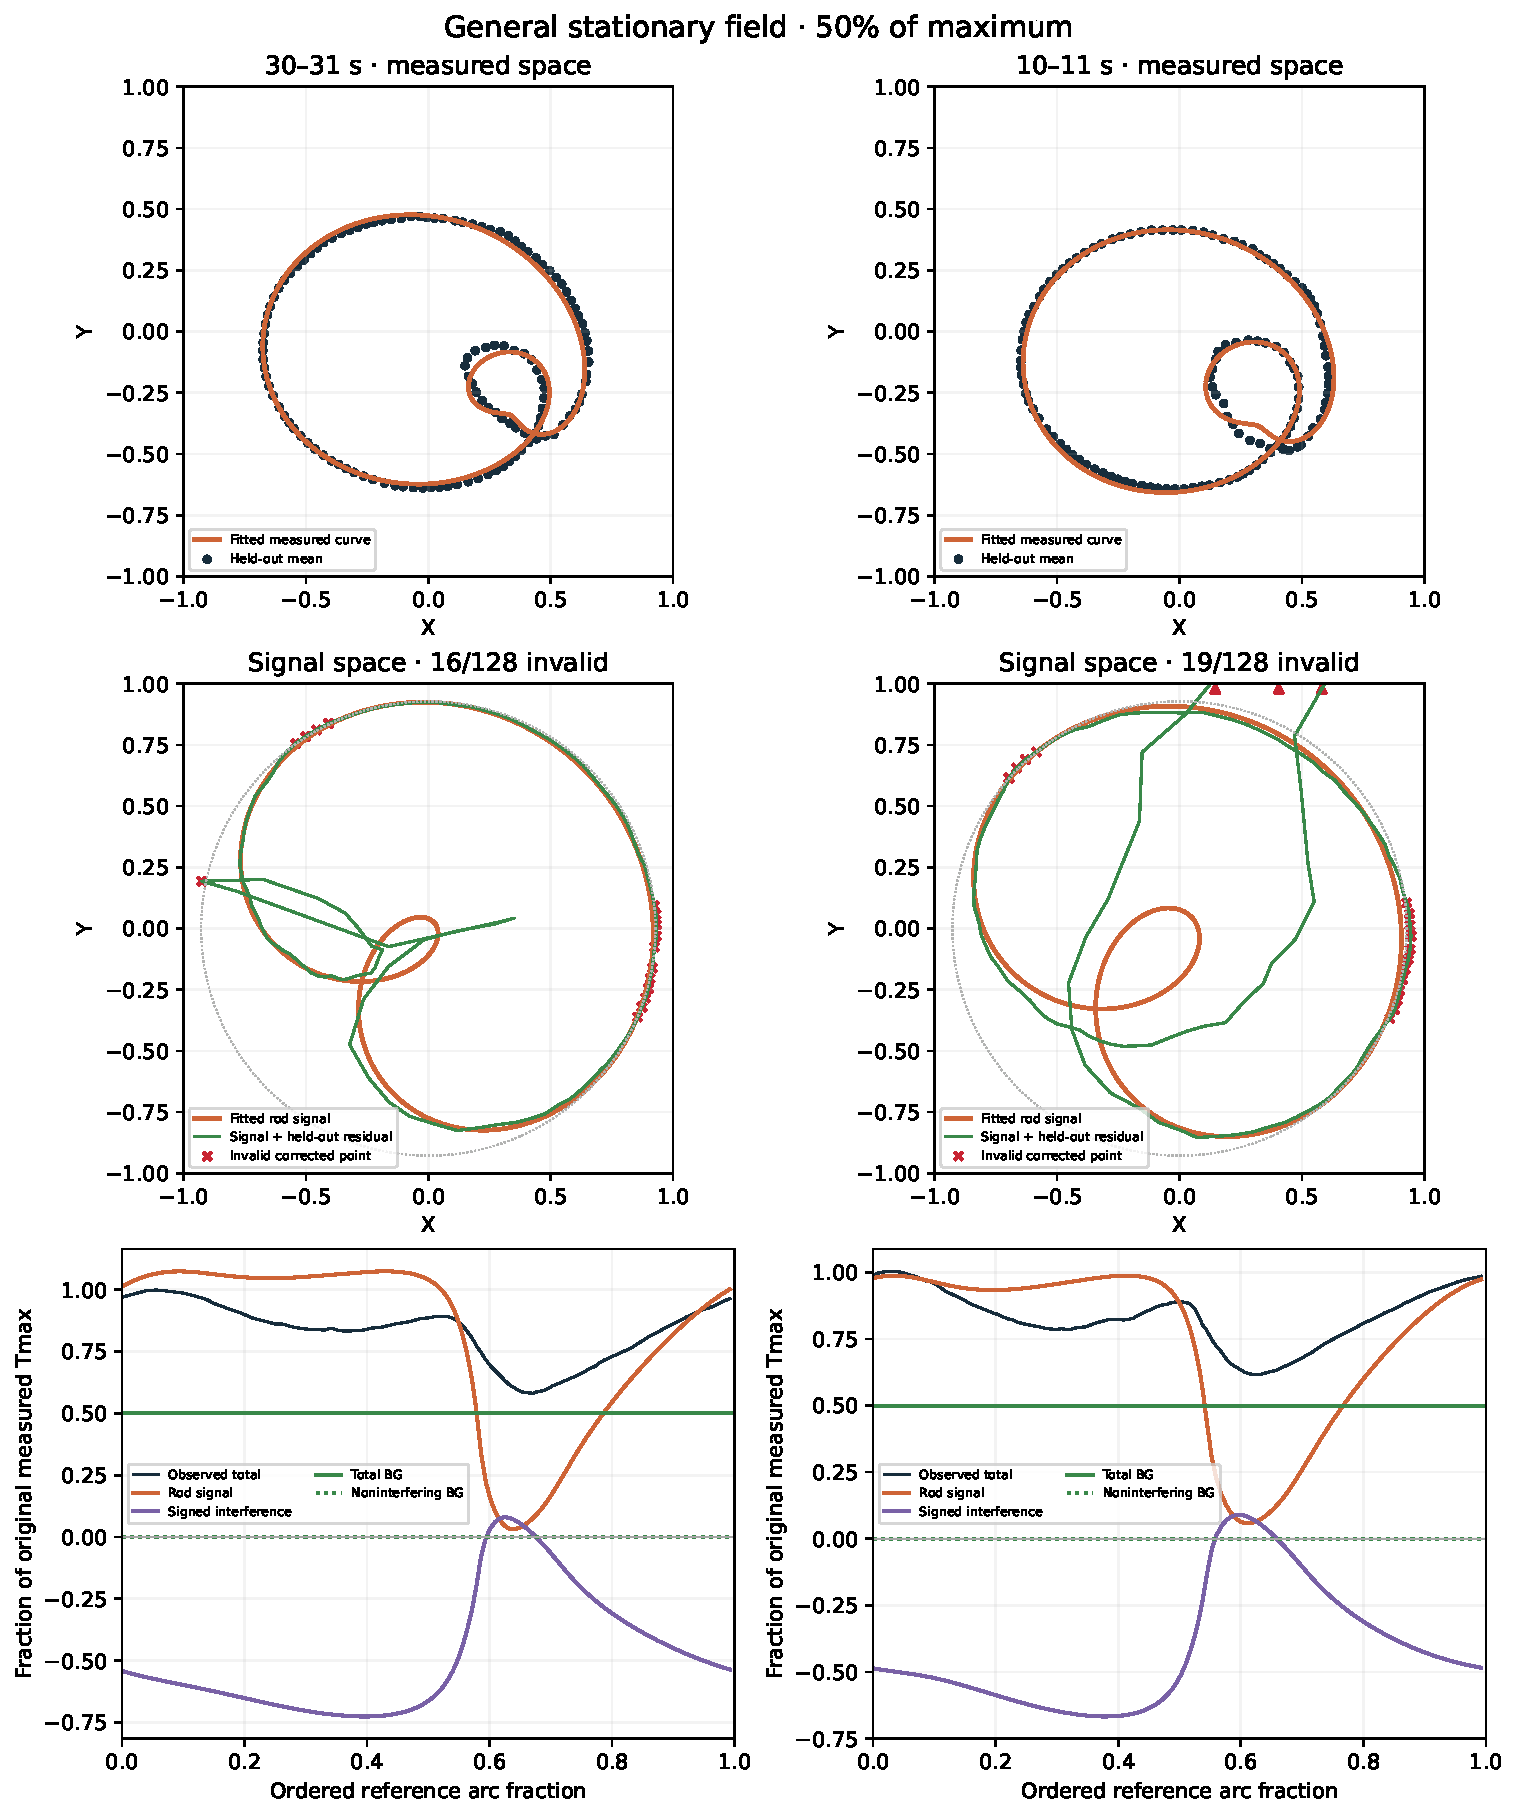
\includegraphics[width=\linewidth,height=.9\textheight,keepaspectratio]{figures/general_50pct.pdf}
\newpage
\subsection{Representative sphere diagnostic: 10\% of maximum}
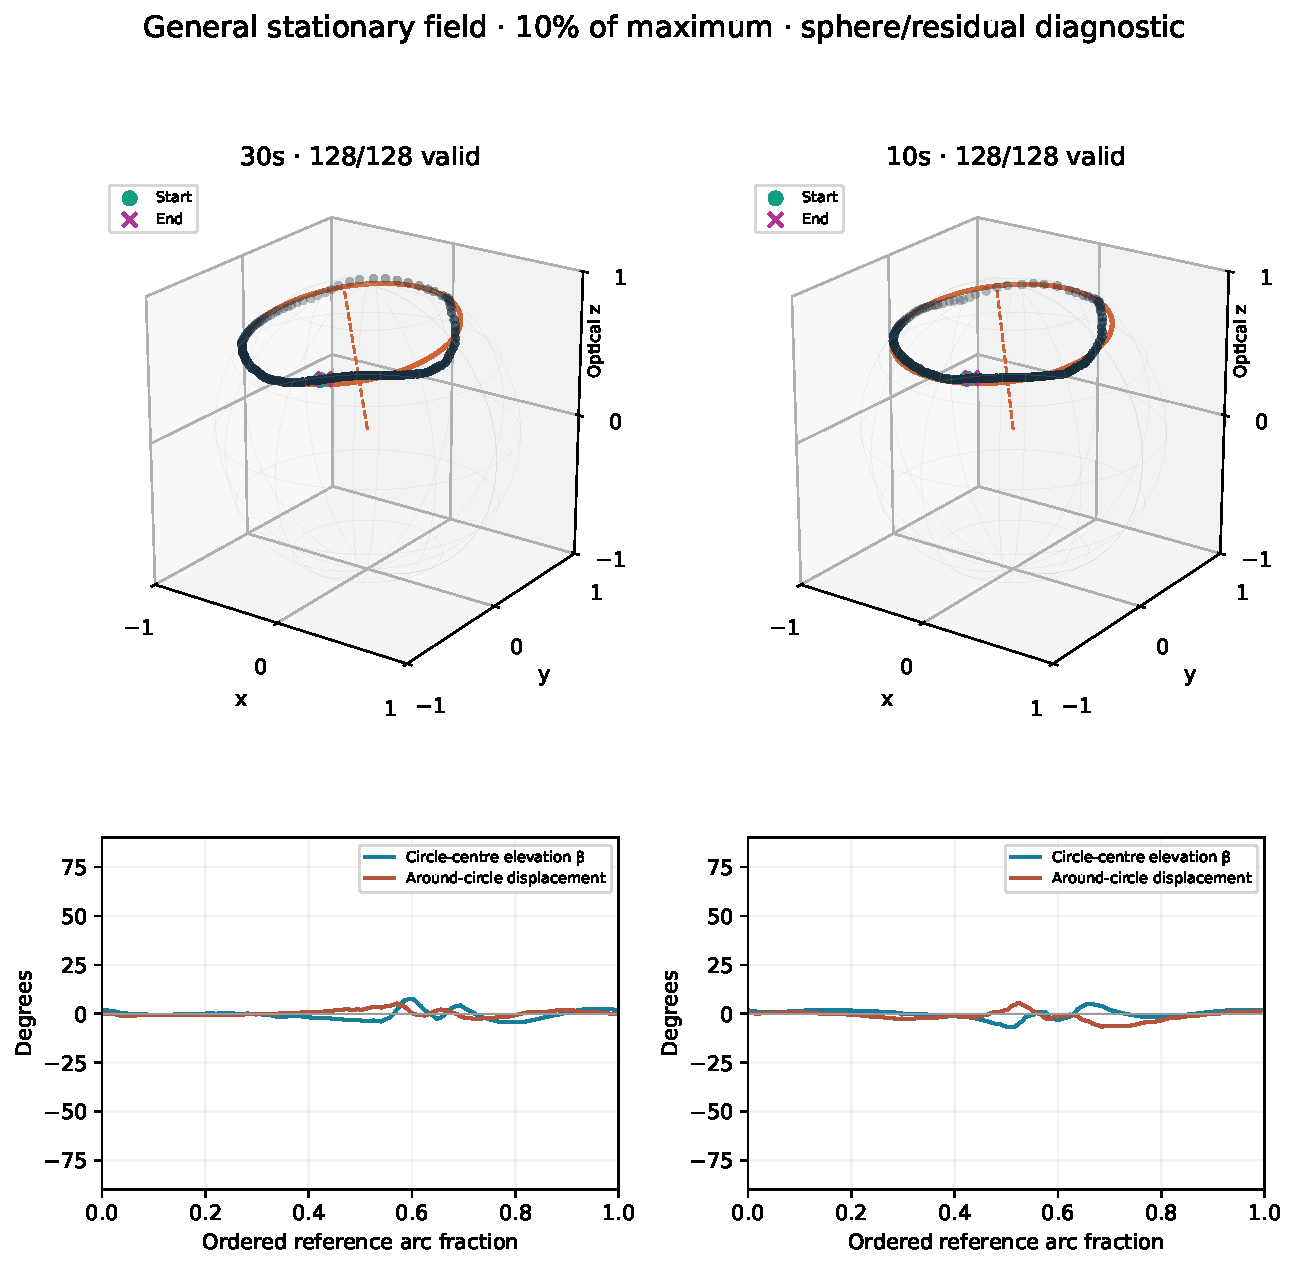
\includegraphics[width=\linewidth,height=.82\textheight,keepaspectratio]{figures/general_sphere.pdf}
30s: 128/128 valid; matched geodesic RMS 2.94$^\circ$; oriented closure mismatch 0.00$^\circ$.\par
10s: 128/128 valid; matched geodesic RMS 3.49$^\circ$; oriented closure mismatch 0.00$^\circ$.\par
\newpage
\subsection{Local cone-referenced angular residual: 10\% of maximum}\label{local:general}
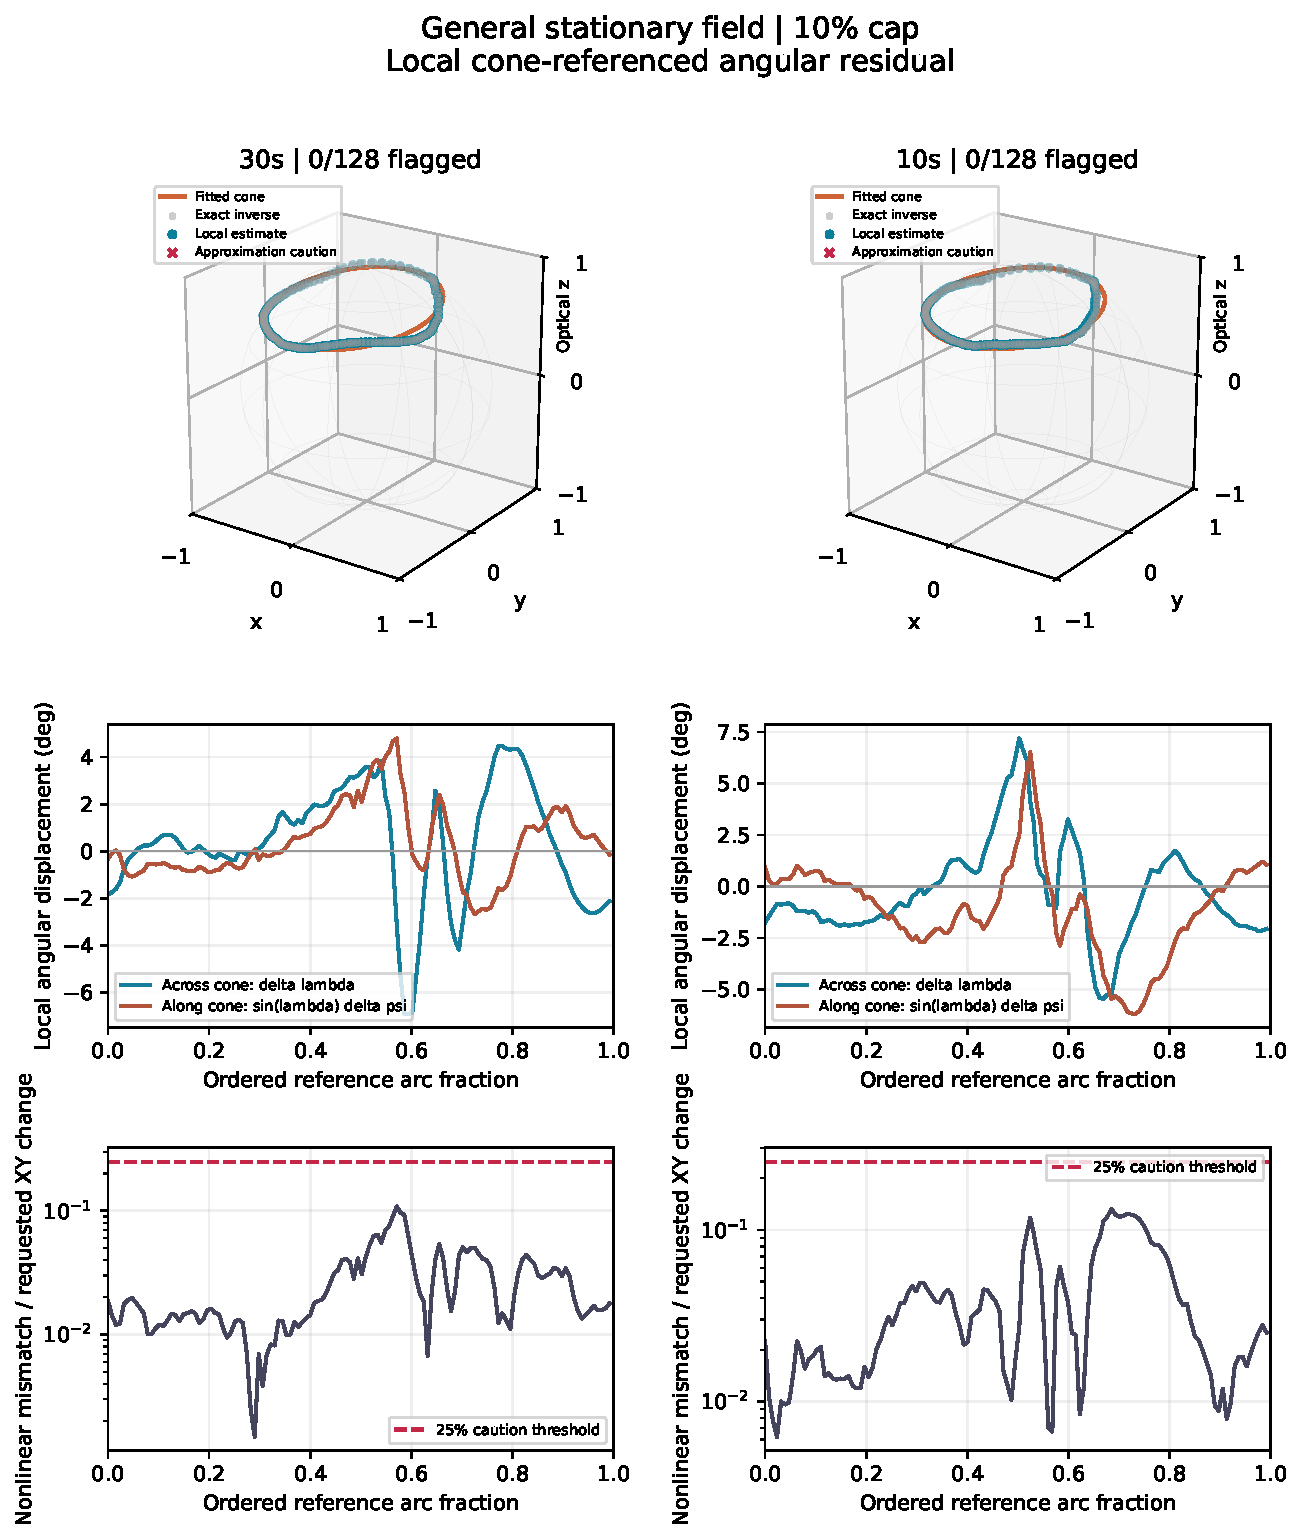
\includegraphics[width=\linewidth,height=.86\textheight,keepaspectratio]{local_residual/general.pdf}
30s: local angular RMS 2.91$^\circ$; 0/128 caution flags; median nonlinear mismatch ratio 0.018.\par
10s: local angular RMS 3.48$^\circ$; 0/128 caution flags; median nonlinear mismatch ratio 0.028.\par
\newpage
\section{Hole-edge field}
\[\mathbf{E}_b=\sum_{m=1}^{6}b_m\mathbf{U}_m,\qquad
\mathbf{U}_m\propto e^{-(\rho-0.38)^2/(2w^2)}\{1,\cos\varphi,\sin\varphi\},\quad w=0.10\ \mathrm{NA}.\]
Each scalar shape is used in two transverse polarizations and orthonormalized. Fit six complex coefficients plus a noninterfering Stokes background (fifteen shared plus ten local parameters). The width is fixed, not fitted. This draft adds the noninterfering component to the earlier pure edge-field surrogate. It tests a restricted pupil pattern, not a full model of multiple reflection or hole-edge scattering.
\textbf{Total fitted continuous parameters across both windows: 25.} The three pre-estimated gain adjustments are additional calibration parameters, held fixed here.
\begin{longtable}{llrrrrrr}\toprule
Budget & Window & BG\% & Meas.RMS & Signal RMS & Bad(train/test) & Max $r$ & Conv.\\\midrule\endhead
uncapped & 30s & 24.5 & 0.0249 & 0.0403 & 9/11 & 0.940 & yes \\
uncapped & 10s & 24.4 & 0.0274 & 0.0438 & 0/0 & 0.909 & yes \\
5pct & 30s & 5.0 & 0.0567 & 0.0735 & 0/0 & 0.718 & yes \\
5pct & 10s & 5.0 & 0.0572 & 0.0724 & 0/0 & 0.702 & yes \\
10pct & 30s & 10.0 & 0.0441 & 0.0624 & 0/0 & 0.774 & yes \\
10pct & 10s & 10.0 & 0.0460 & 0.0623 & 0/0 & 0.748 & yes \\
20pct & 30s & 20.0 & 0.0269 & 0.0434 & 0/0 & 0.919 & NO \\
20pct & 10s & 19.9 & 0.0303 & 0.0453 & 0/0 & 0.880 & NO \\
30pct & 30s & 24.5 & 0.0249 & 0.0403 & 9/11 & 0.940 & yes \\
30pct & 10s & 24.4 & 0.0274 & 0.0438 & 0/0 & 0.909 & yes \\
\bottomrule\end{longtable}
\begin{longtable}{llrrrr}\toprule
Budget & Window & Signal\% range & Cross\% range & Noninterf.BG\% & Fitted folded $\theta$\\\midrule\endhead
uncapped & 30s & 26.7--82.4 & -14.3--3.5 & 0.0 & 33.0--67.9$^\circ$ \\
uncapped & 10s & 31.6--79.4 & -13.9--3.5 & 0.0 & 36.9--67.6$^\circ$ \\
5pct & 30s & 42.4--104.1 & -5.3--2.4 & 0.0 & 30.3--50.7$^\circ$ \\
5pct & 10s & 48.5--99.9 & -5.1--2.5 & 0.0 & 32.0--48.4$^\circ$ \\
10pct & 30s & 35.3--97.8 & -7.0--3.4 & 0.0 & 30.3--55.0$^\circ$ \\
10pct & 10s & 42.4--94.2 & -6.8--3.5 & 0.0 & 32.6--52.0$^\circ$ \\
20pct & 30s & 27.4--86.0 & -11.2--3.6 & 0.0 & 31.9--65.2$^\circ$ \\
20pct & 10s & 33.9--83.8 & -11.0--3.8 & 0.0 & 35.0--61.6$^\circ$ \\
30pct & 30s & 26.7--82.4 & -14.3--3.5 & 0.0 & 33.0--67.9$^\circ$ \\
30pct & 10s & 31.6--79.4 & -13.9--3.5 & 0.0 & 36.9--67.6$^\circ$ \\
\bottomrule\end{longtable}
\textbf{Per-channel constant background, percent of measured maximum:}
\begin{longtable}{llrrrr}\toprule
Budget & Window & $B_0$ & $B_{90}$ & $B_{45}$ & $B_{135}$\\\midrule\endhead
uncapped & 30s & 7.98 & 4.26 & 3.75 & 8.50\\
uncapped & 10s & 7.95 & 4.24 & 3.73 & 8.46\\
5pct & 30s & 1.98 & 0.52 & 0.52 & 1.98\\
5pct & 10s & 1.97 & 0.52 & 0.52 & 1.97\\
10pct & 30s & 3.96 & 1.04 & 0.95 & 4.05\\
10pct & 10s & 3.94 & 1.03 & 0.95 & 4.03\\
20pct & 30s & 7.54 & 2.46 & 2.40 & 7.60\\
20pct & 10s & 7.51 & 2.45 & 2.39 & 7.56\\
30pct & 30s & 7.98 & 4.26 & 3.75 & 8.50\\
30pct & 10s & 7.95 & 4.24 & 3.73 & 8.46\\
\bottomrule\end{longtable}
\newpage
\subsection{No BG-power cap}\label{case:edge:uncapped}
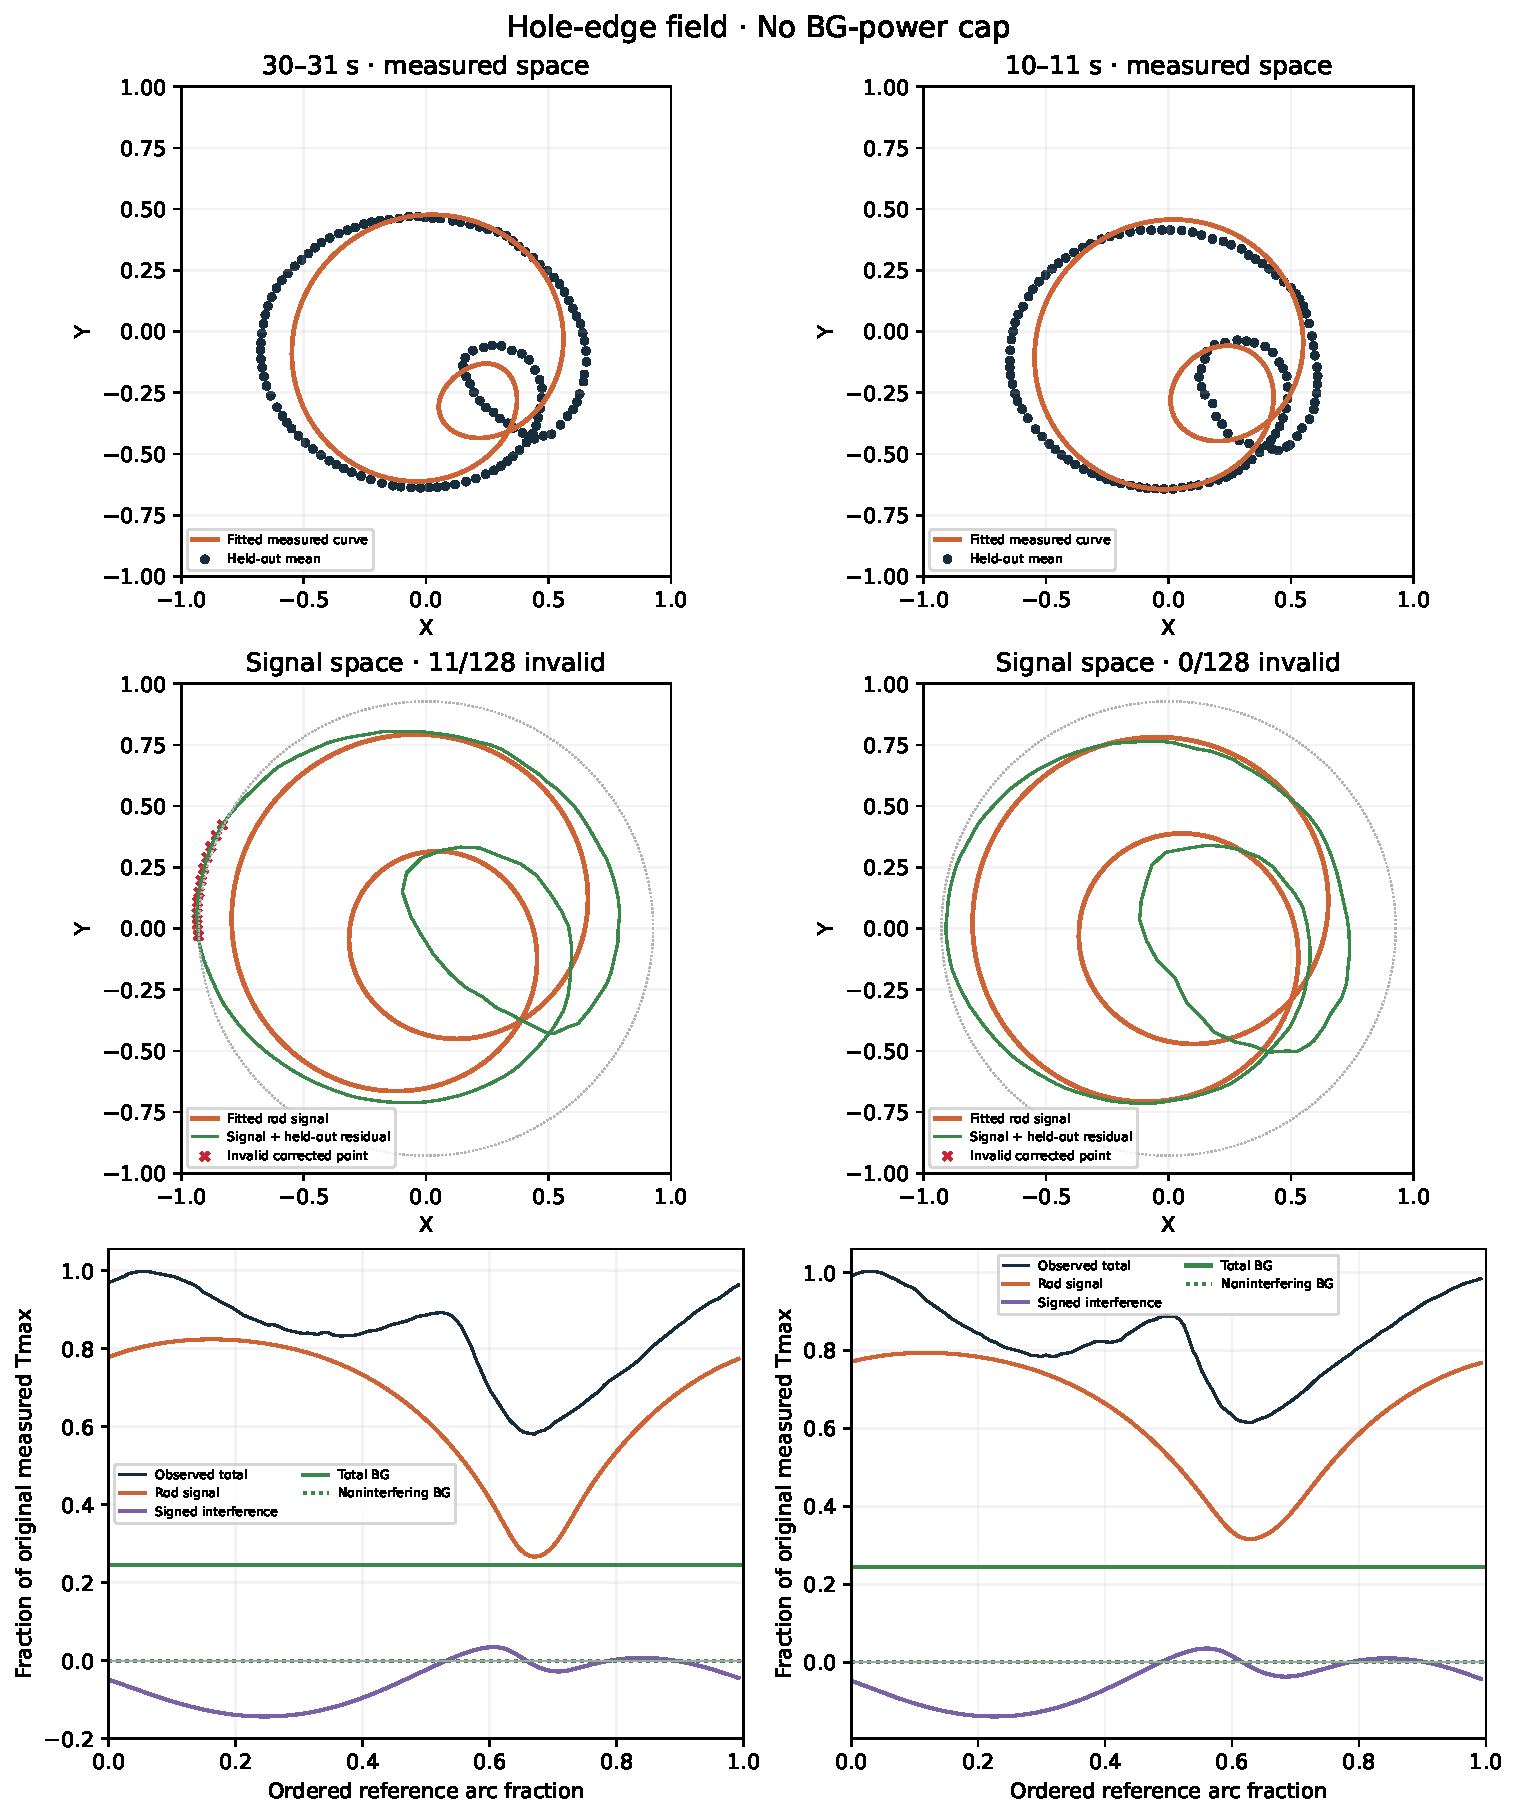
\includegraphics[width=\linewidth,height=.9\textheight,keepaspectratio]{figures/edge_uncapped.pdf}
\newpage
\subsection{5\% of maximum}\label{case:edge:5pct}
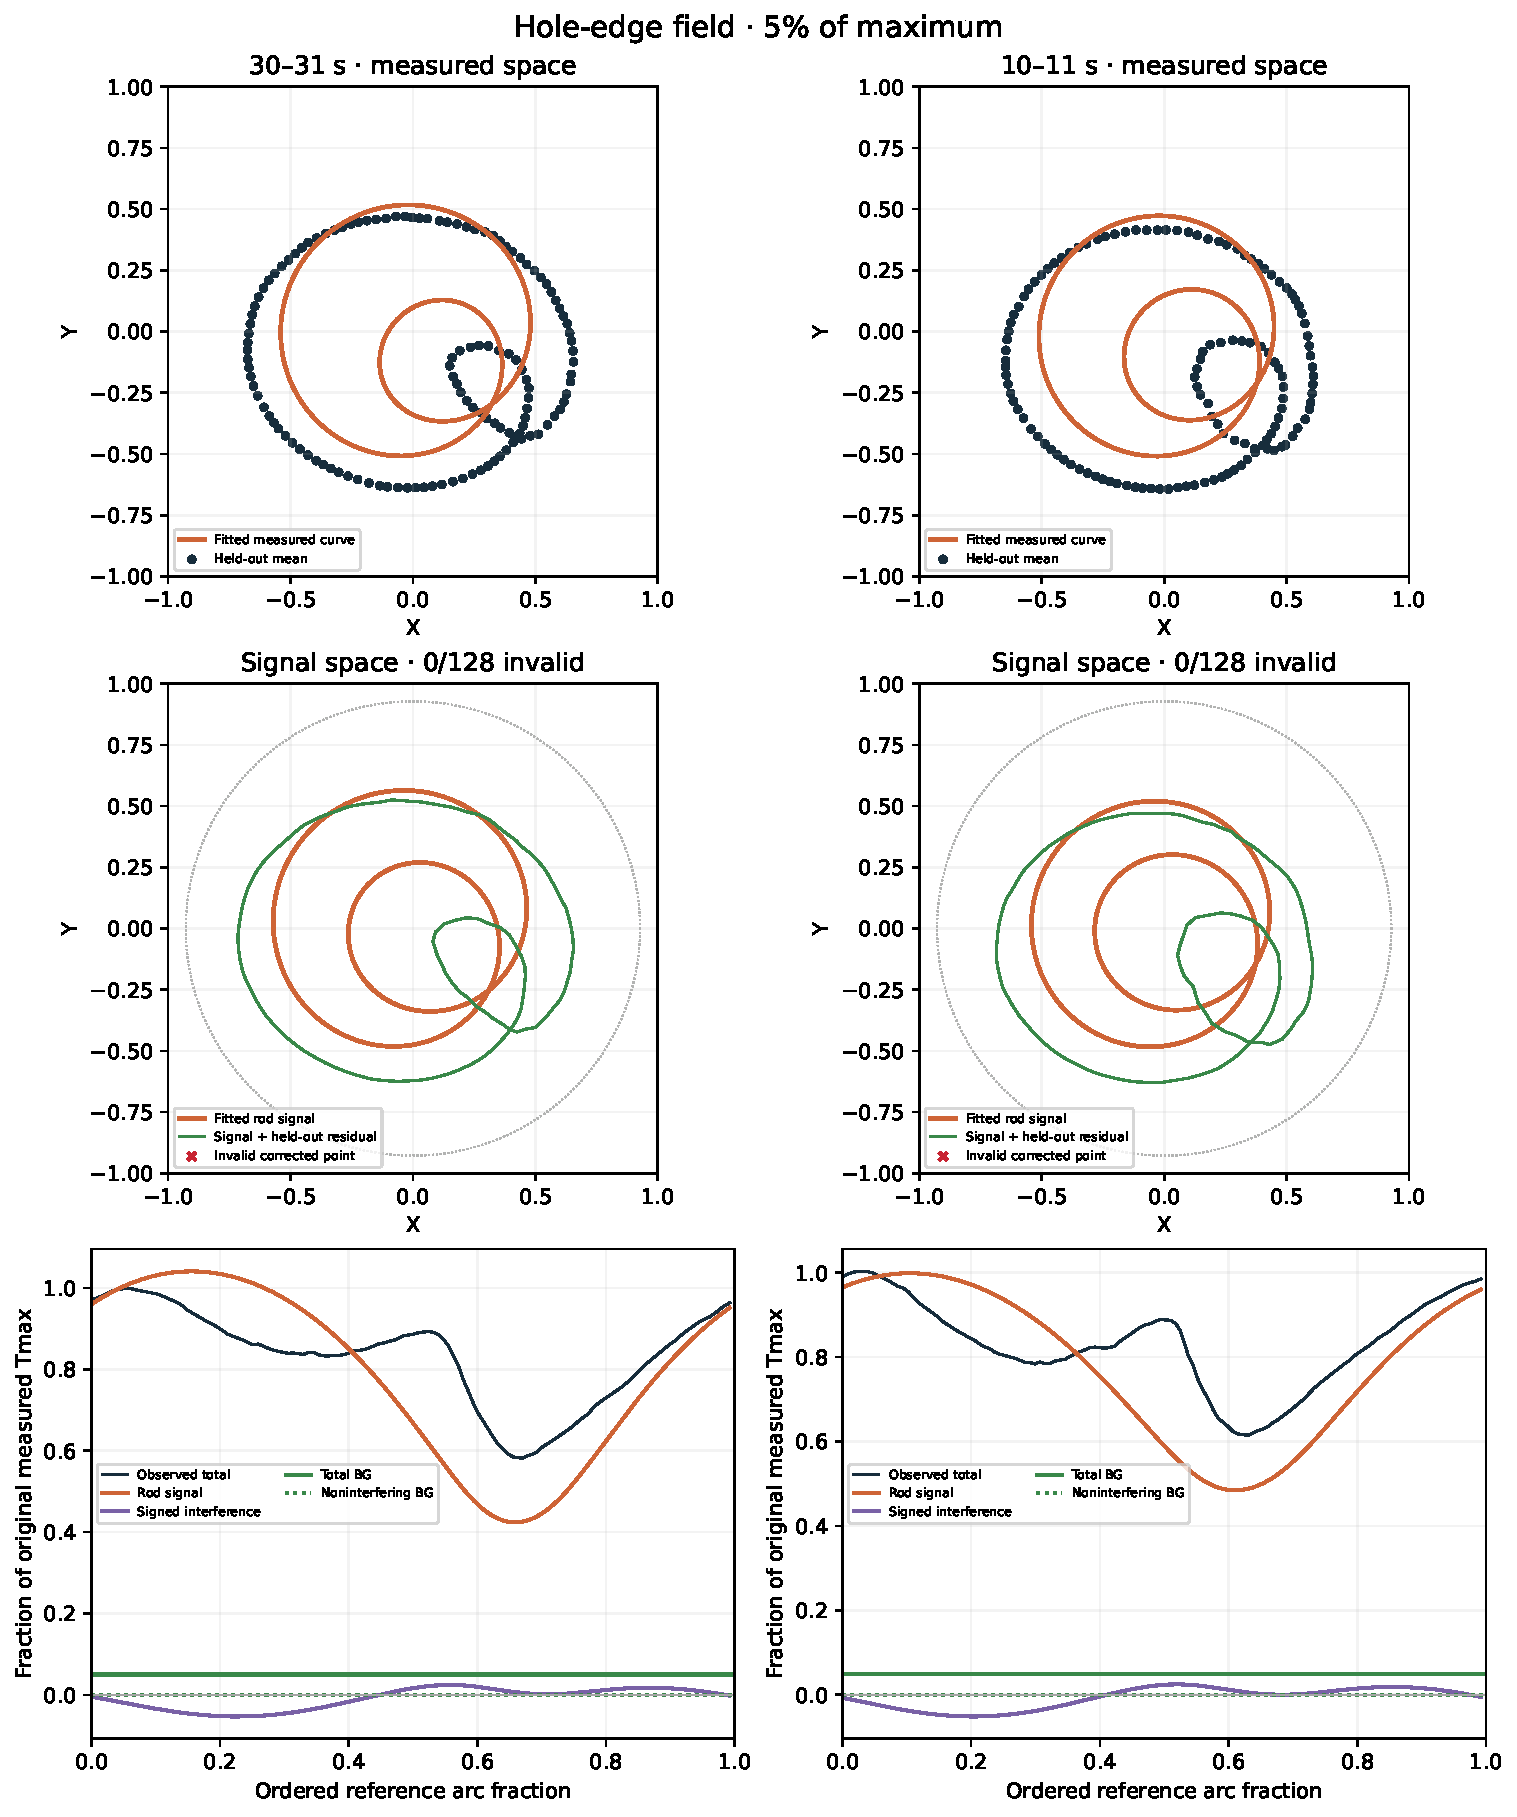
\includegraphics[width=\linewidth,height=.9\textheight,keepaspectratio]{figures/edge_5pct.pdf}
\newpage
\subsection{10\% of maximum}\label{case:edge:10pct}
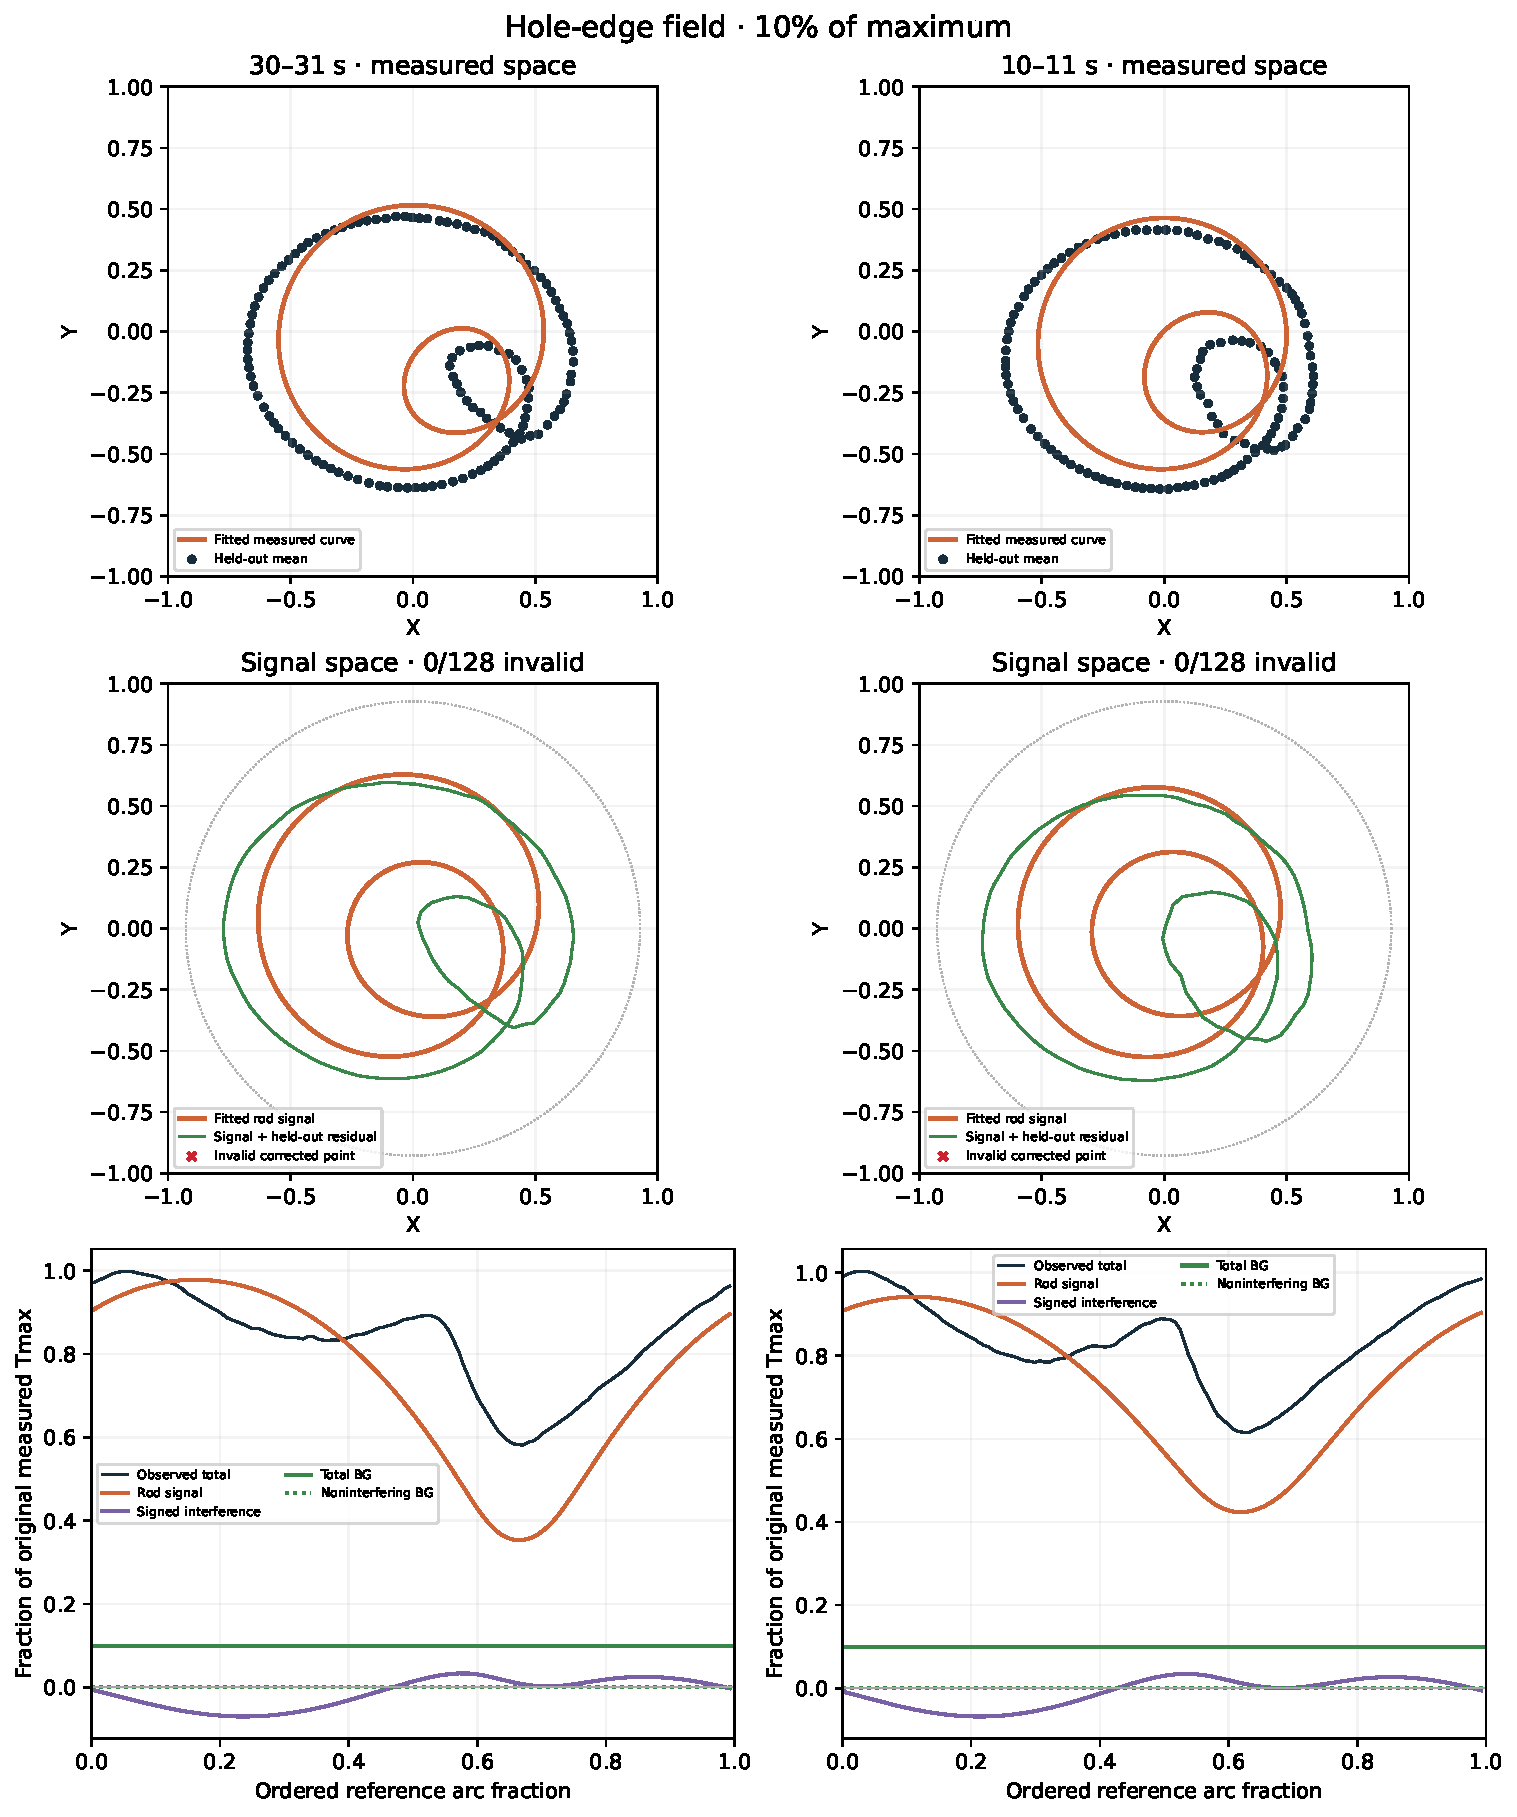
\includegraphics[width=\linewidth,height=.9\textheight,keepaspectratio]{figures/edge_10pct.pdf}
\newpage
\subsection{20\% of maximum}\label{case:edge:20pct}
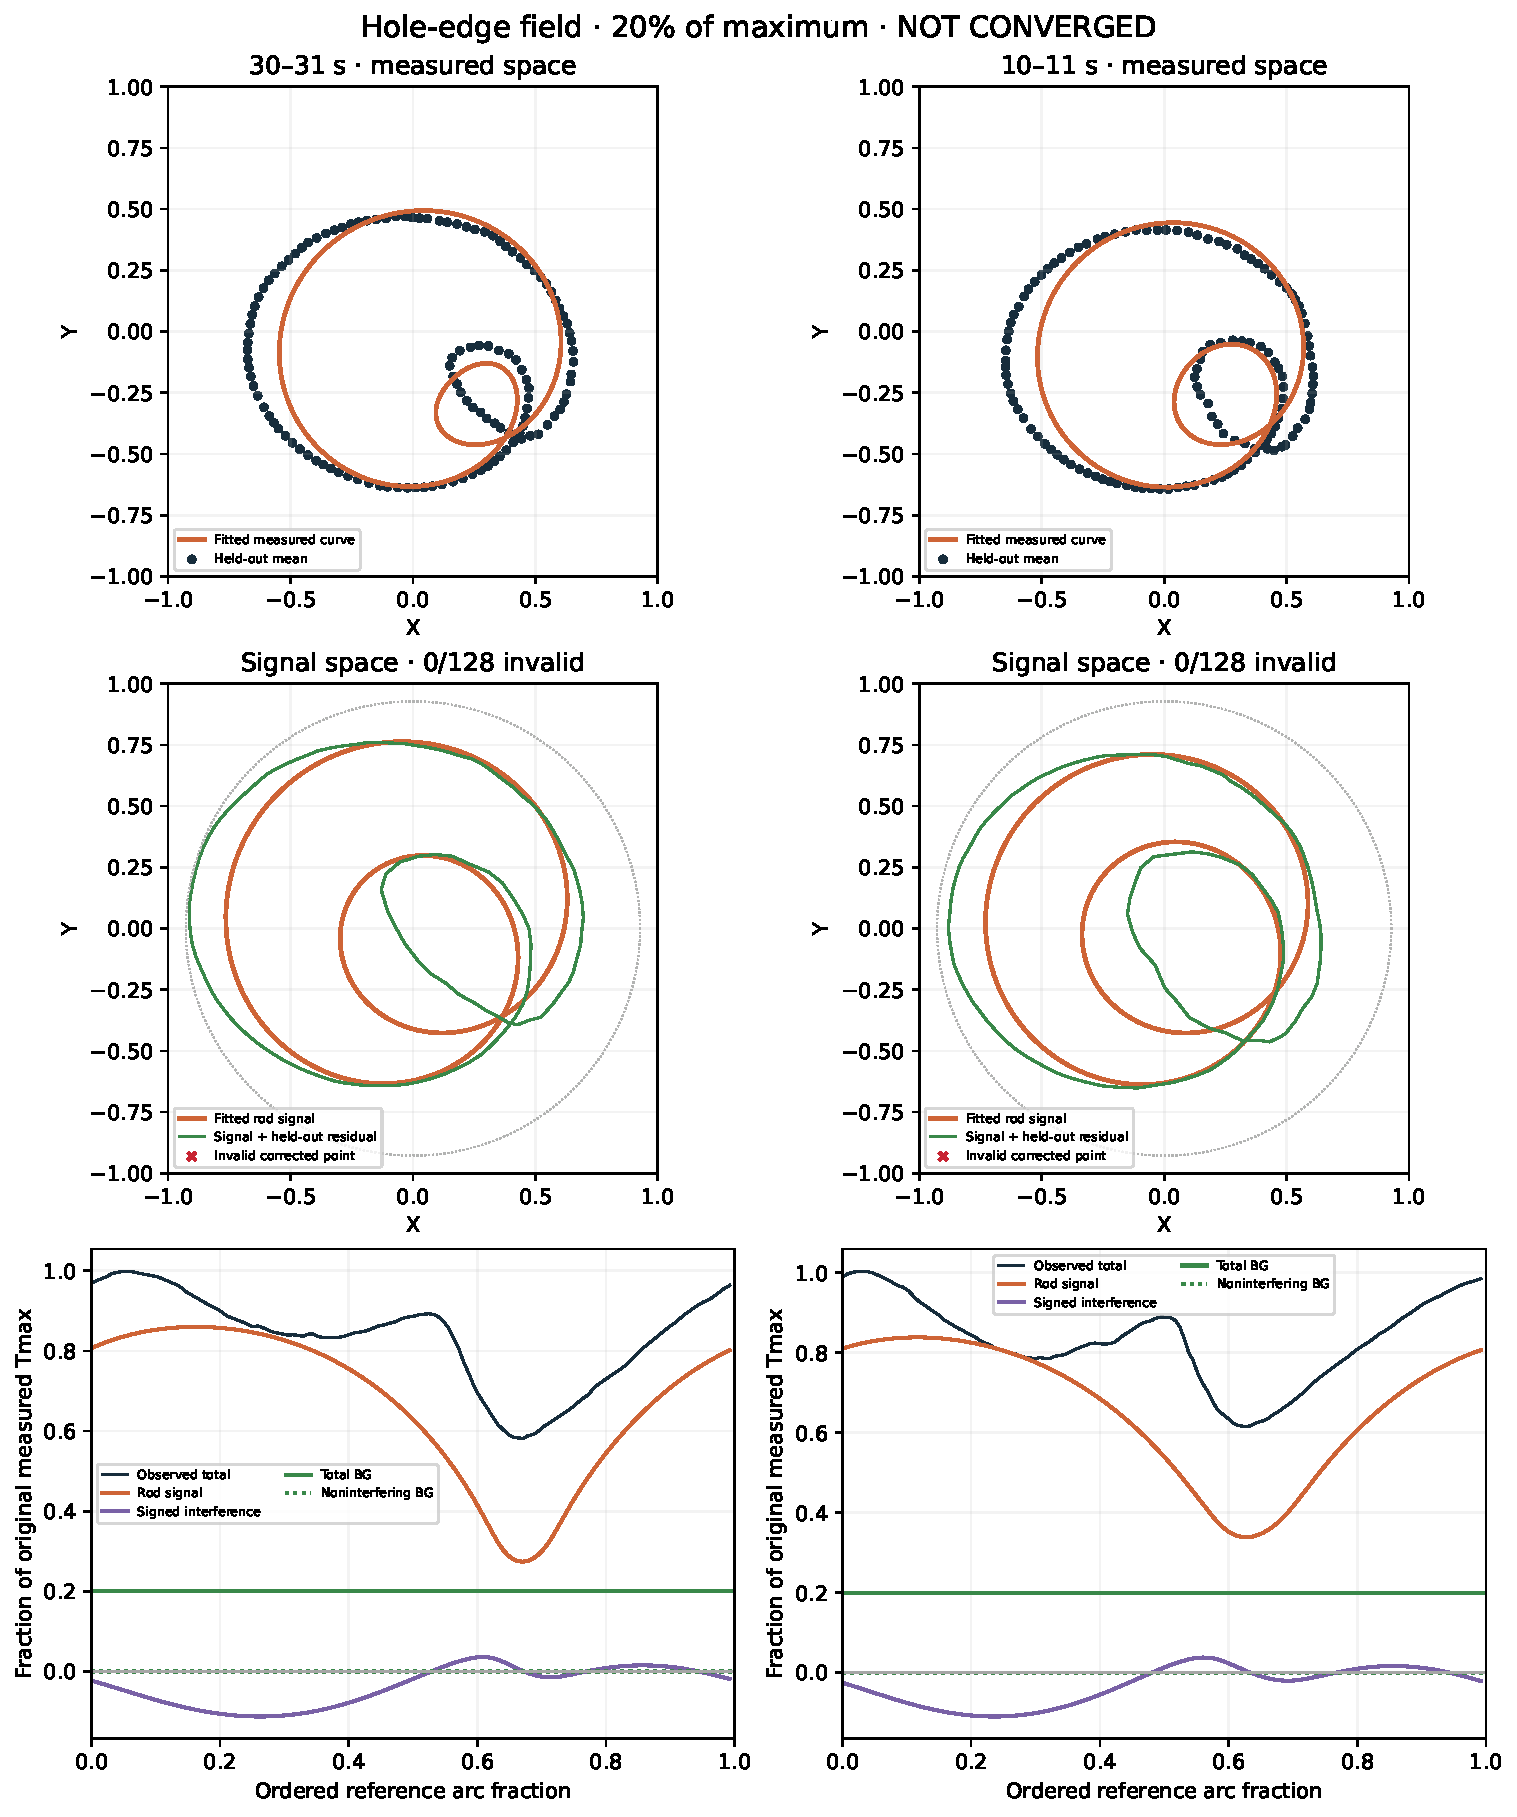
\includegraphics[width=\linewidth,height=.9\textheight,keepaspectratio]{figures/edge_20pct.pdf}
\newpage
\subsection{30\% of maximum}\label{case:edge:30pct}
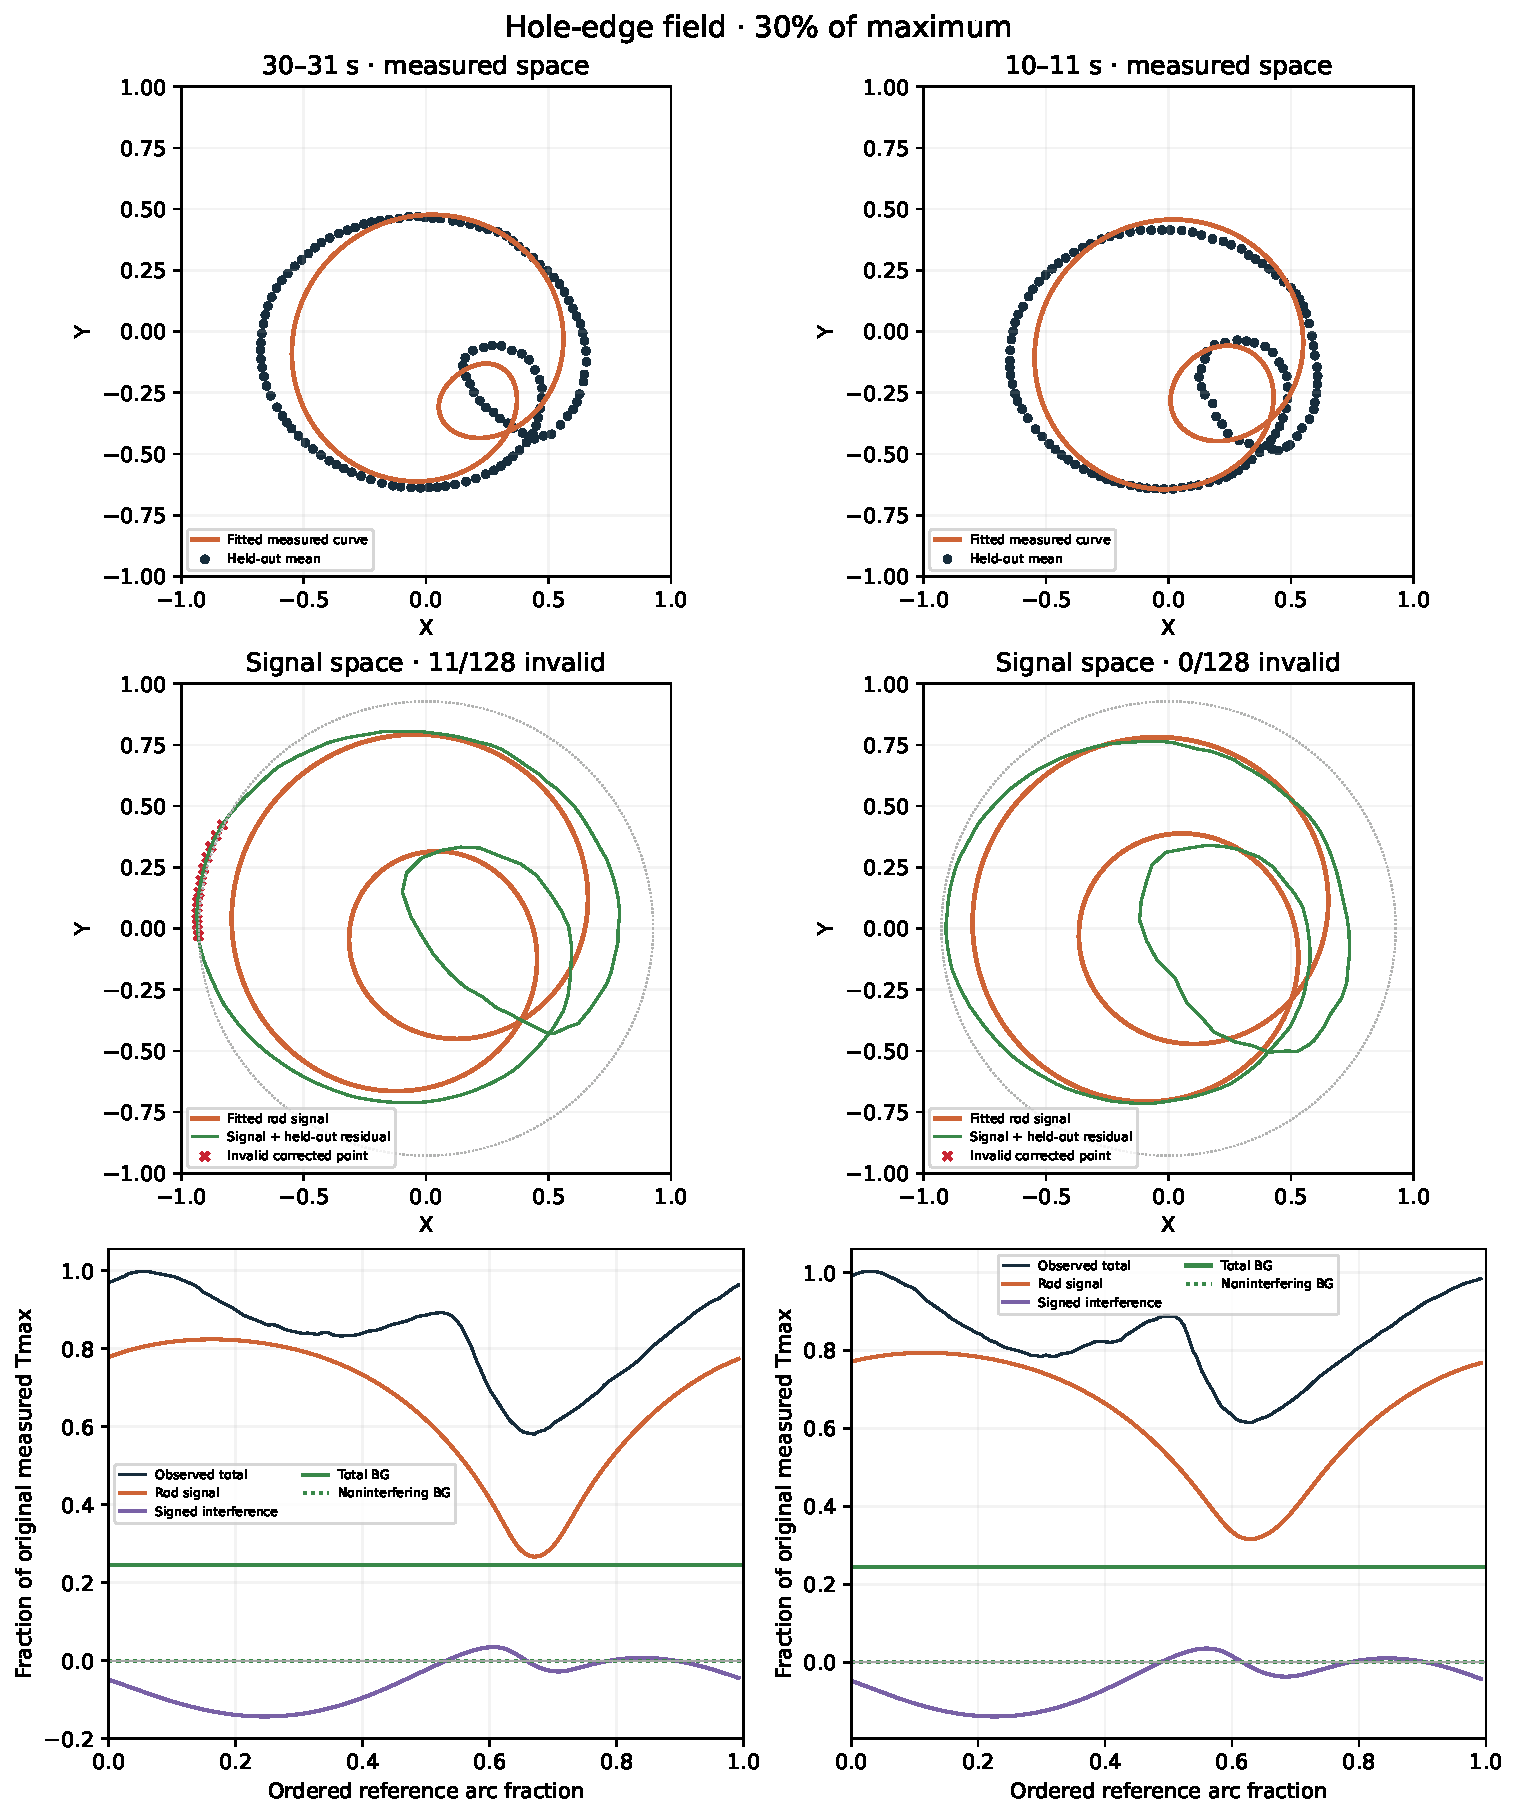
\includegraphics[width=\linewidth,height=.9\textheight,keepaspectratio]{figures/edge_30pct.pdf}
\newpage
\subsection{Representative sphere diagnostic: 10\% of maximum}
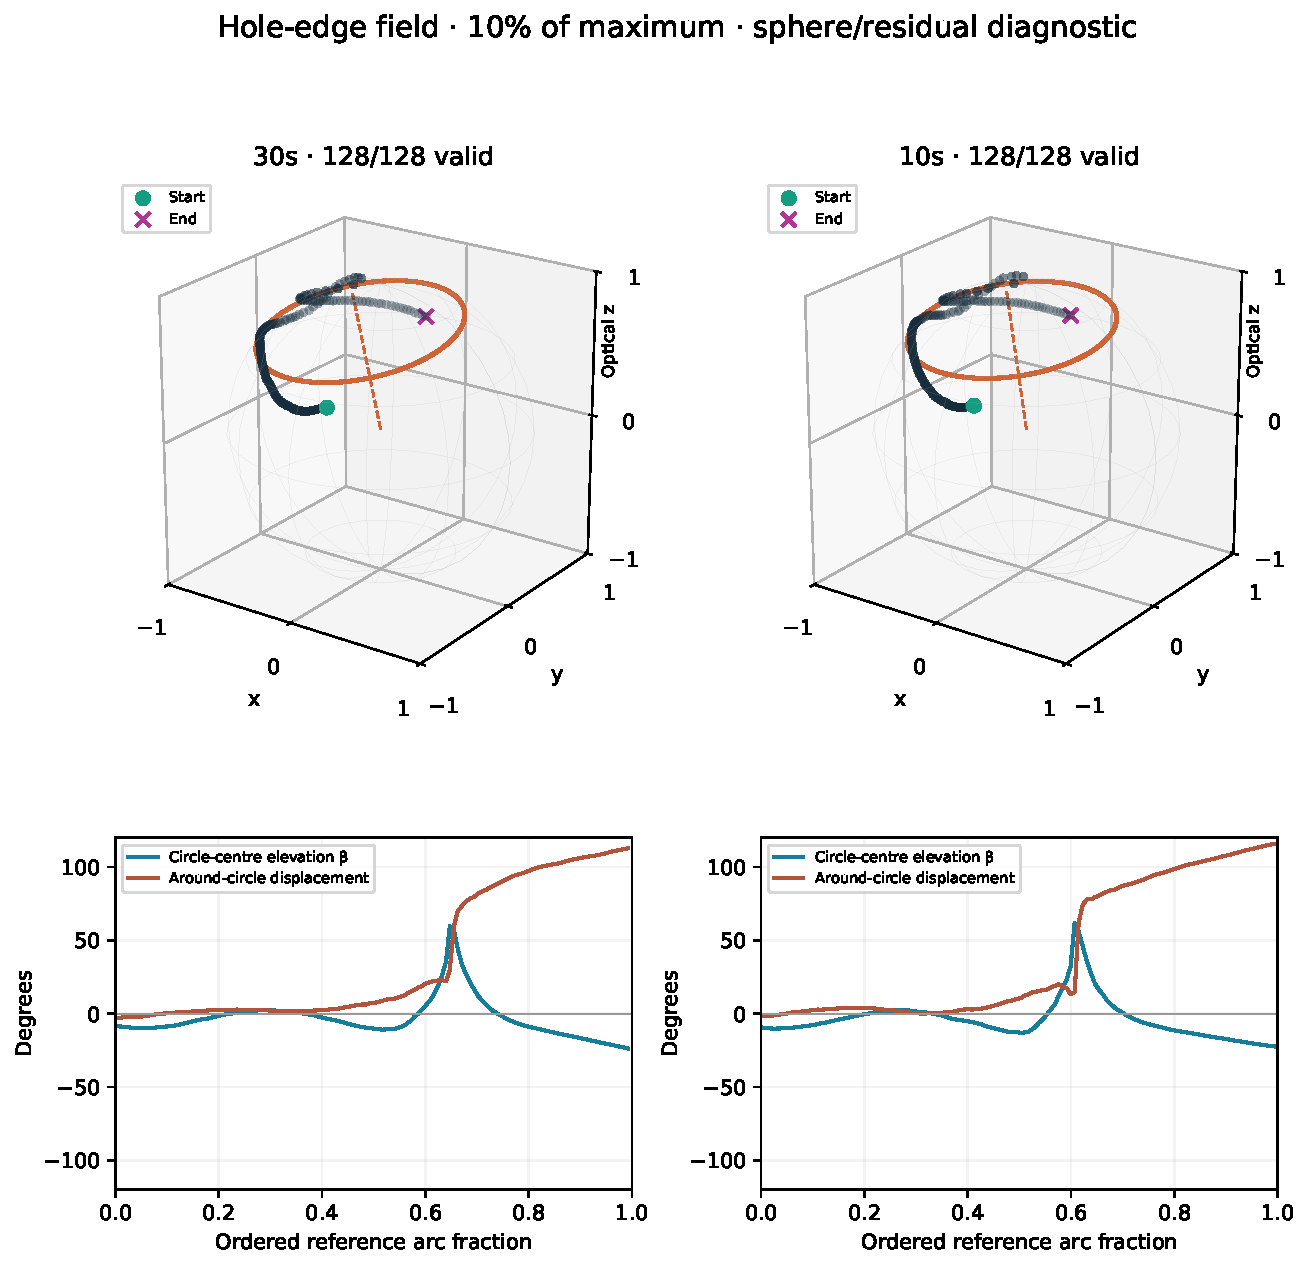
\includegraphics[width=\linewidth,height=.82\textheight,keepaspectratio]{figures/edge_sphere.pdf}
30s: 128/128 valid; matched geodesic RMS 53.36$^\circ$; oriented closure mismatch 123.40$^\circ$.\par
10s: 128/128 valid; matched geodesic RMS 56.20$^\circ$; oriented closure mismatch 121.98$^\circ$.\par
\newpage
\subsection{Local cone-referenced angular residual: 10\% of maximum}\label{local:edge}
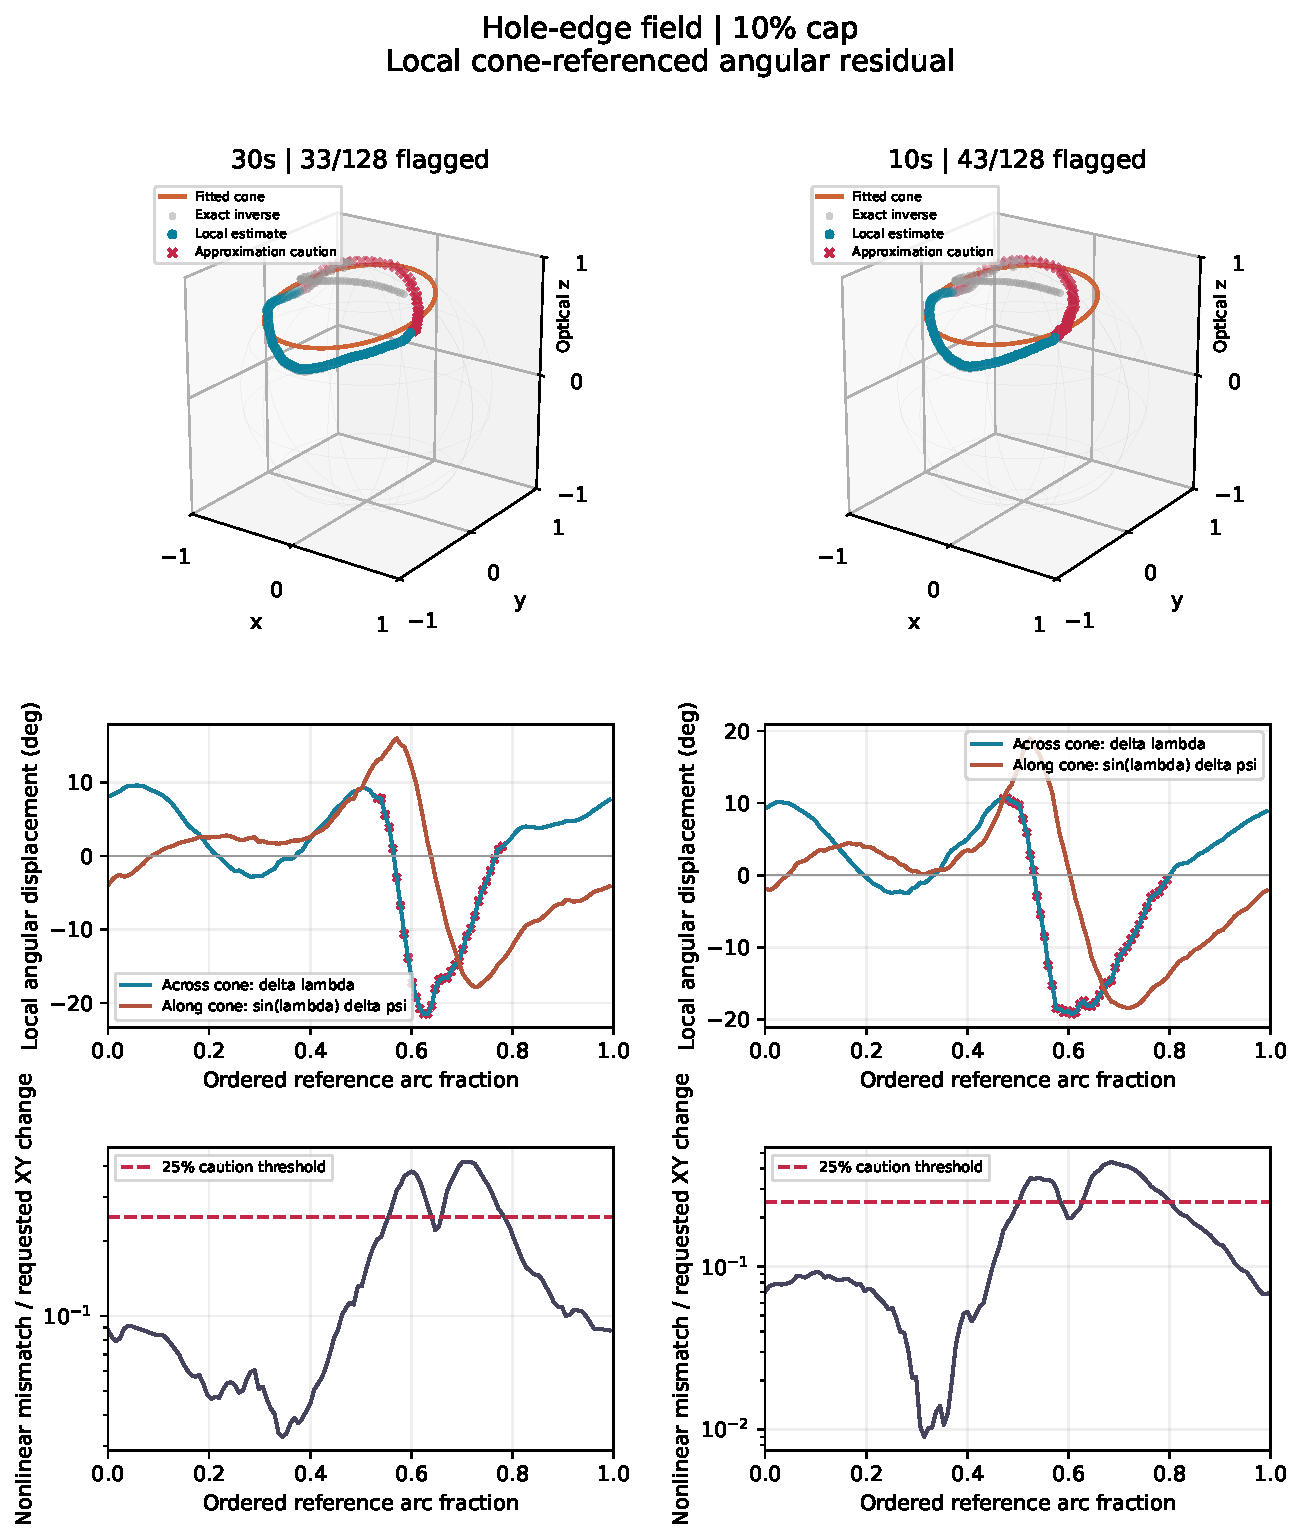
\includegraphics[width=\linewidth,height=.86\textheight,keepaspectratio]{local_residual/edge.pdf}
30s: local angular RMS 11.54$^\circ$; 33/128 caution flags; median nonlinear mismatch ratio 0.093.\par
10s: local angular RMS 12.70$^\circ$; 43/128 caution flags; median nonlinear mismatch ratio 0.094.\par
\newpage
\section{General field with axial motion}
\[z(\chi)=R_h\sin\beta_{axis}\cos(\chi+\eta),\qquad 0\leq R_h\leq0.30\ \mu\mathrm m.\]
Use the general field with an orientation-linked axial trajectory, fitting $R_h,\eta$ per window in addition to the 33 stationary parameters. The 300 nm orbit-radius bound is a sensitivity assumption, not a measured hook length. The mean plane is fixed at the assumed excitation waist.
\[F(z)=[1+(z/z_R)^2]^{-1/2},\quad z_R=2\ \mu\mathrm m,\quad
S_i=a_0^2\sin^2\theta F(z)^2Q_i.\]
The pupil overlap carries the phase factor\[\exp\{\mathrm i(2\pi/\lambda_0)[n_w+\sqrt{n_w^2-\rho^2}]z\},\qquad \lambda_0=633\ \mathrm{nm}.\]The excitation also contributes the Gouy phase $-\arctan(z/z_R)$. Thus $I_{\mathrm{int},i}$ changes with both orientation and height. Background power stays constant. This retains the earlier bounded axial-phase/focus model; it is not a full finite-detector image-space defocus calculation.
\textbf{Total fitted continuous parameters across both windows: 37.} The three pre-estimated gain adjustments are additional calibration parameters, held fixed here.
\begin{longtable}{llrrrrrr}\toprule
Budget & Window & BG\% & Meas.RMS & Signal RMS & Bad(train/test) & Max $r$ & Conv.\\\midrule\endhead
uncapped & 30s & 54.9 & 0.0042 & 0.0146 & 0/0 & 0.927 & yes \\
uncapped & 10s & 54.7 & 0.0084 & 0.0221 & 0/0 & 0.916 & yes \\
5pct & 30s & 5.0 & 0.0146 & 0.0175 & 0/0 & 0.650 & NO \\
5pct & 10s & 5.0 & 0.0185 & 0.0218 & 0/0 & 0.660 & NO \\
10pct & 30s & 10.0 & 0.0060 & 0.0075 & 0/0 & 0.658 & yes \\
10pct & 10s & 10.0 & 0.0098 & 0.0121 & 0/0 & 0.622 & yes \\
20pct & 30s & 18.5 & 0.0049 & 0.0073 & 0/0 & 0.748 & NO \\
20pct & 10s & 18.4 & 0.0090 & 0.0126 & 0/0 & 0.715 & NO \\
30pct & 30s & 30.0 & 0.0047 & 0.0093 & 0/0 & 0.815 & yes \\
30pct & 10s & 29.9 & 0.0087 & 0.0154 & 0/0 & 0.794 & yes \\
40pct & 30s & 40.0 & 0.0045 & 0.0082 & 0/7 & 0.940 & yes \\
40pct & 10s & 39.8 & 0.0083 & 0.0145 & 7/8 & 0.936 & yes \\
\bottomrule\end{longtable}
\begin{longtable}{llrrrr}\toprule
Budget & Window & Signal\% range & Cross\% range & Noninterf.BG\% & Fitted folded $\theta$\\\midrule\endhead
uncapped & 30s & 9.2--86.5 & -54.5---0.8 & 0.0 & 19.8--82.2$^\circ$ \\
uncapped & 10s & 13.3--89.7 & -61.5--0.2 & 0.0 & 23.5--81.0$^\circ$ \\
5pct & 30s & 43.8--98.7 & -18.5--13.0 & 0.0 & 32.5--52.3$^\circ$ \\
5pct & 10s & 50.0--93.8 & -18.2--14.3 & 0.0 & 34.7--50.2$^\circ$ \\
10pct & 30s & 43.5--92.6 & -17.1--10.6 & 0.0 & 35.2--55.4$^\circ$ \\
10pct & 10s & 49.3--88.9 & -16.9--10.7 & 0.0 & 37.3--53.2$^\circ$ \\
20pct & 30s & 31.4--96.5 & -22.7--22.2 & 0.0 & 30.8--60.7$^\circ$ \\
20pct & 10s & 35.5--96.7 & -24.9--22.9 & 0.0 & 32.1--58.7$^\circ$ \\
30pct & 30s & 21.7--91.3 & -29.3--19.5 & 0.0 & 27.6--66.4$^\circ$ \\
30pct & 10s & 25.2--93.0 & -33.4--20.9 & 0.0 & 29.2--65.0$^\circ$ \\
40pct & 30s & 22.8--81.3 & -33.9--5.7 & 0.0 & 33.2--83.8$^\circ$ \\
40pct & 10s & 25.5--82.1 & -39.9--6.9 & 0.0 & 35.2--85.3$^\circ$ \\
\bottomrule\end{longtable}
\textbf{Per-channel constant background, percent of measured maximum:}
\begin{longtable}{llrrrr}\toprule
Budget & Window & $B_0$ & $B_{90}$ & $B_{45}$ & $B_{135}$\\\midrule\endhead
uncapped & 30s & 15.42 & 12.04 & 9.21 & 18.25\\
uncapped & 10s & 15.35 & 11.99 & 9.17 & 18.17\\
5pct & 30s & 1.83 & 0.67 & 0.64 & 1.86\\
5pct & 10s & 1.83 & 0.66 & 0.63 & 1.85\\
10pct & 30s & 3.86 & 1.14 & 1.04 & 3.96\\
10pct & 10s & 3.84 & 1.14 & 1.04 & 3.94\\
20pct & 30s & 7.33 & 1.93 & 1.99 & 7.27\\
20pct & 10s & 7.29 & 1.92 & 1.98 & 7.24\\
30pct & 30s & 10.67 & 4.33 & 3.95 & 11.05\\
30pct & 10s & 10.62 & 4.31 & 3.94 & 10.99\\
40pct & 30s & 11.27 & 8.73 & 7.60 & 12.40\\
40pct & 10s & 11.21 & 8.69 & 7.56 & 12.35\\
\bottomrule\end{longtable}
\textbf{Fitted axial trajectory (sensitivity assumptions, not independent measurements):}\par
\begin{longtable}{llrrr}\toprule Budget & Window & $R_h$ (nm) & $|z|_{max}$ (nm) & $\eta$ (degrees)\\\midrule\endhead
uncapped & 30s & 24.8 & 12.8 & 123.1\\
uncapped & 10s & 31.3 & 15.1 & 152.9\\
5pct & 30s & 220.9 & 37.9 & 153.0\\
5pct & 10s & 299.9 & 40.4 & 151.9\\
10pct & 30s & 218.8 & 38.5 & 133.9\\
10pct & 10s & 300.0 & 41.6 & 142.2\\
20pct & 30s & 110.2 & 28.5 & 138.7\\
20pct & 10s & 132.4 & 30.4 & 156.6\\
30pct & 30s & 66.3 & 22.1 & 138.2\\
30pct & 10s & 79.9 & 24.6 & 160.0\\
40pct & 30s & 38.2 & 16.3 & 126.0\\
40pct & 10s & 41.5 & 17.6 & 154.9\\
\bottomrule\end{longtable}
\newpage
\subsection{No BG-power cap}\label{case:axial:uncapped}
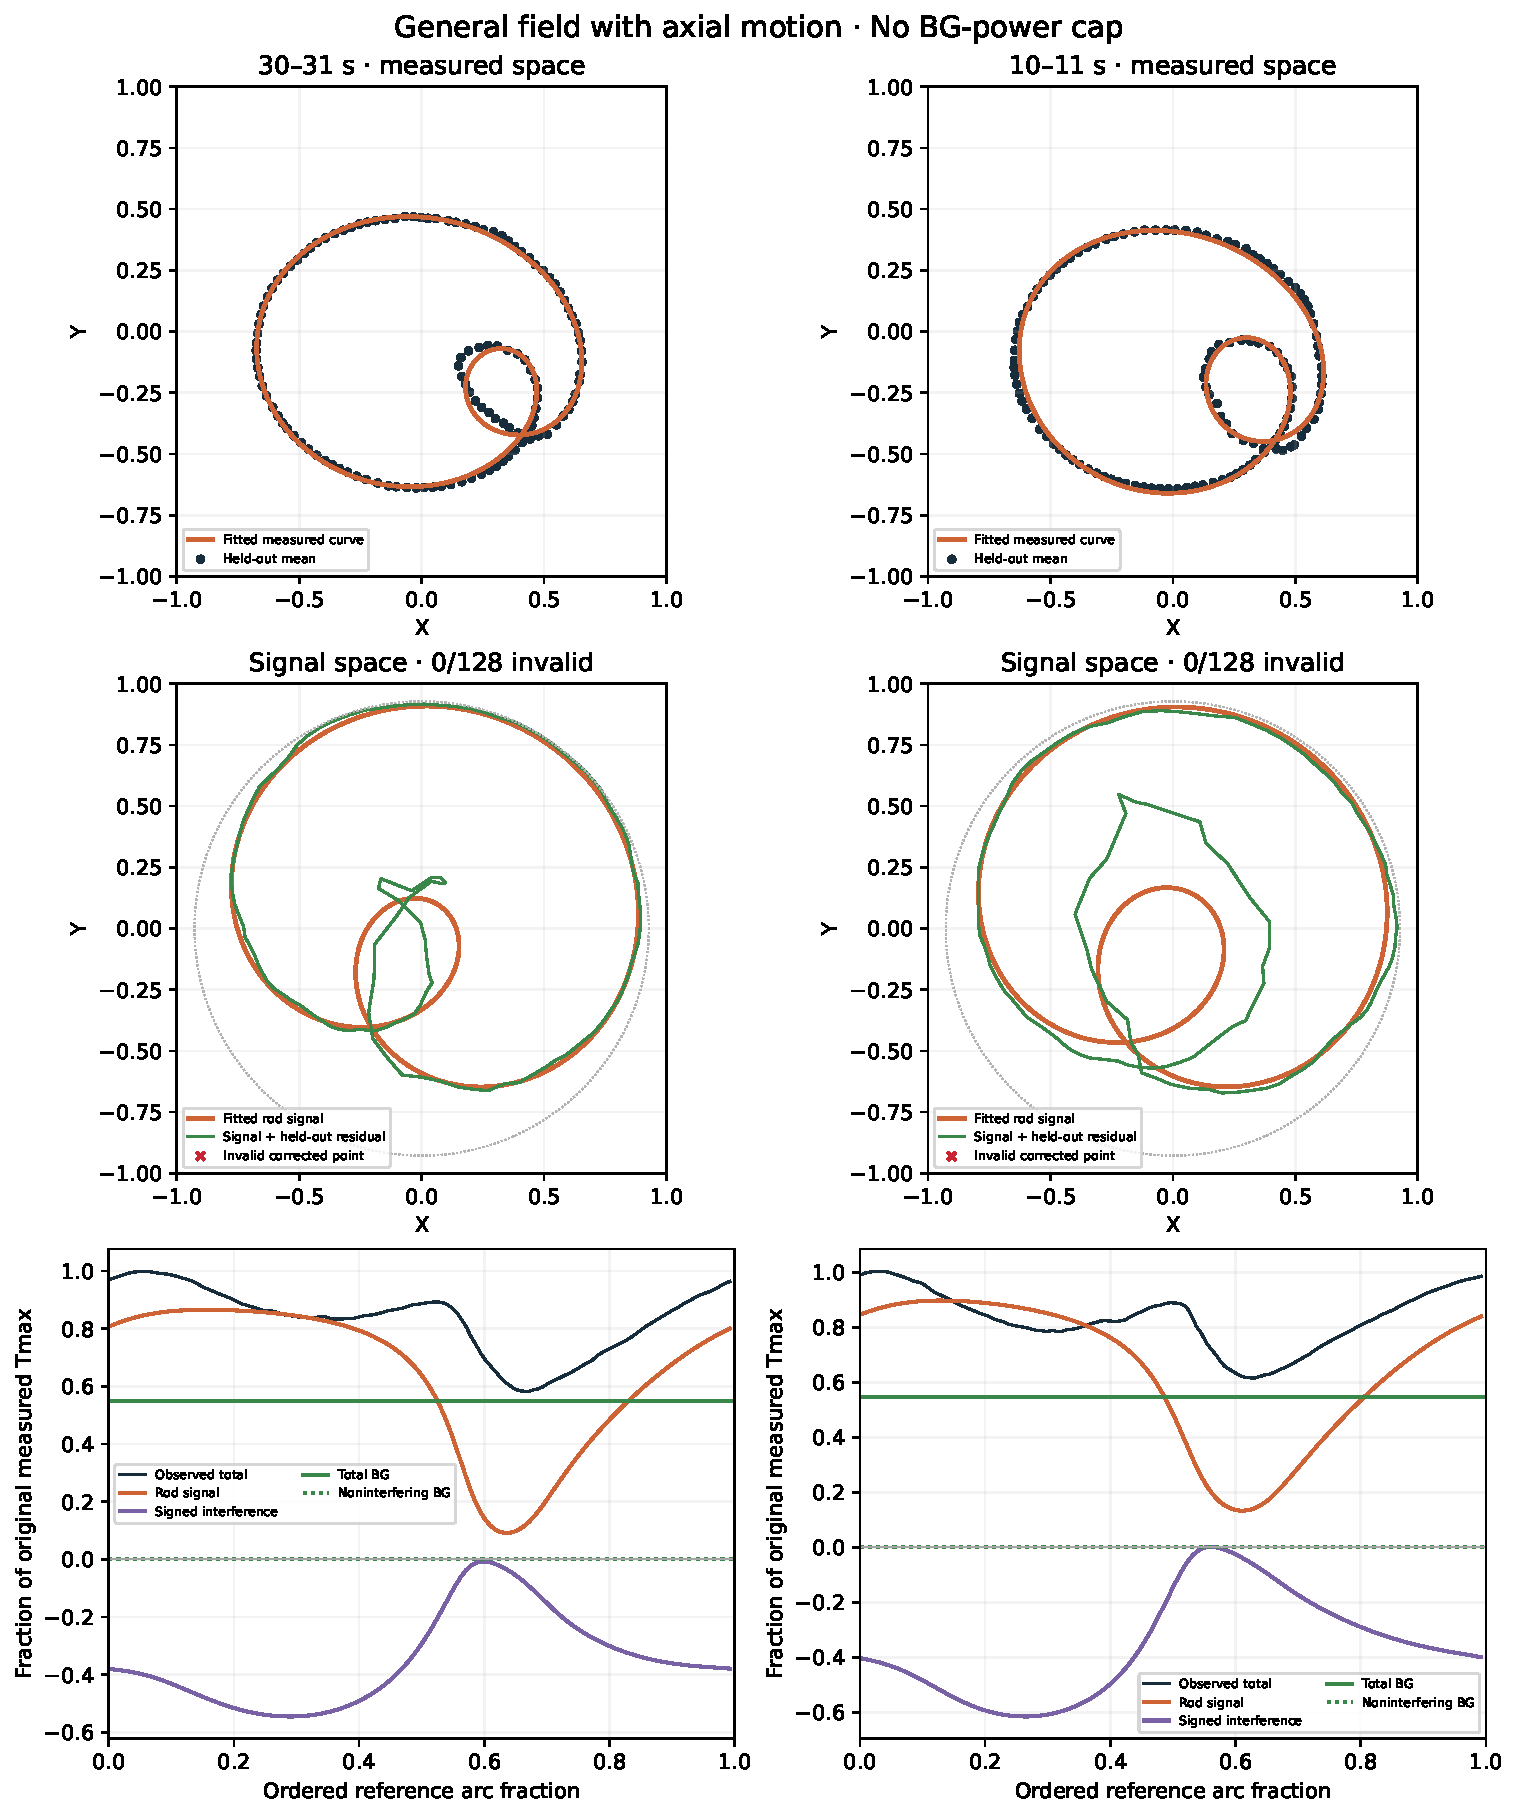
\includegraphics[width=\linewidth,height=.9\textheight,keepaspectratio]{figures/axial_uncapped.pdf}
\newpage
\subsection{5\% of maximum}\label{case:axial:5pct}
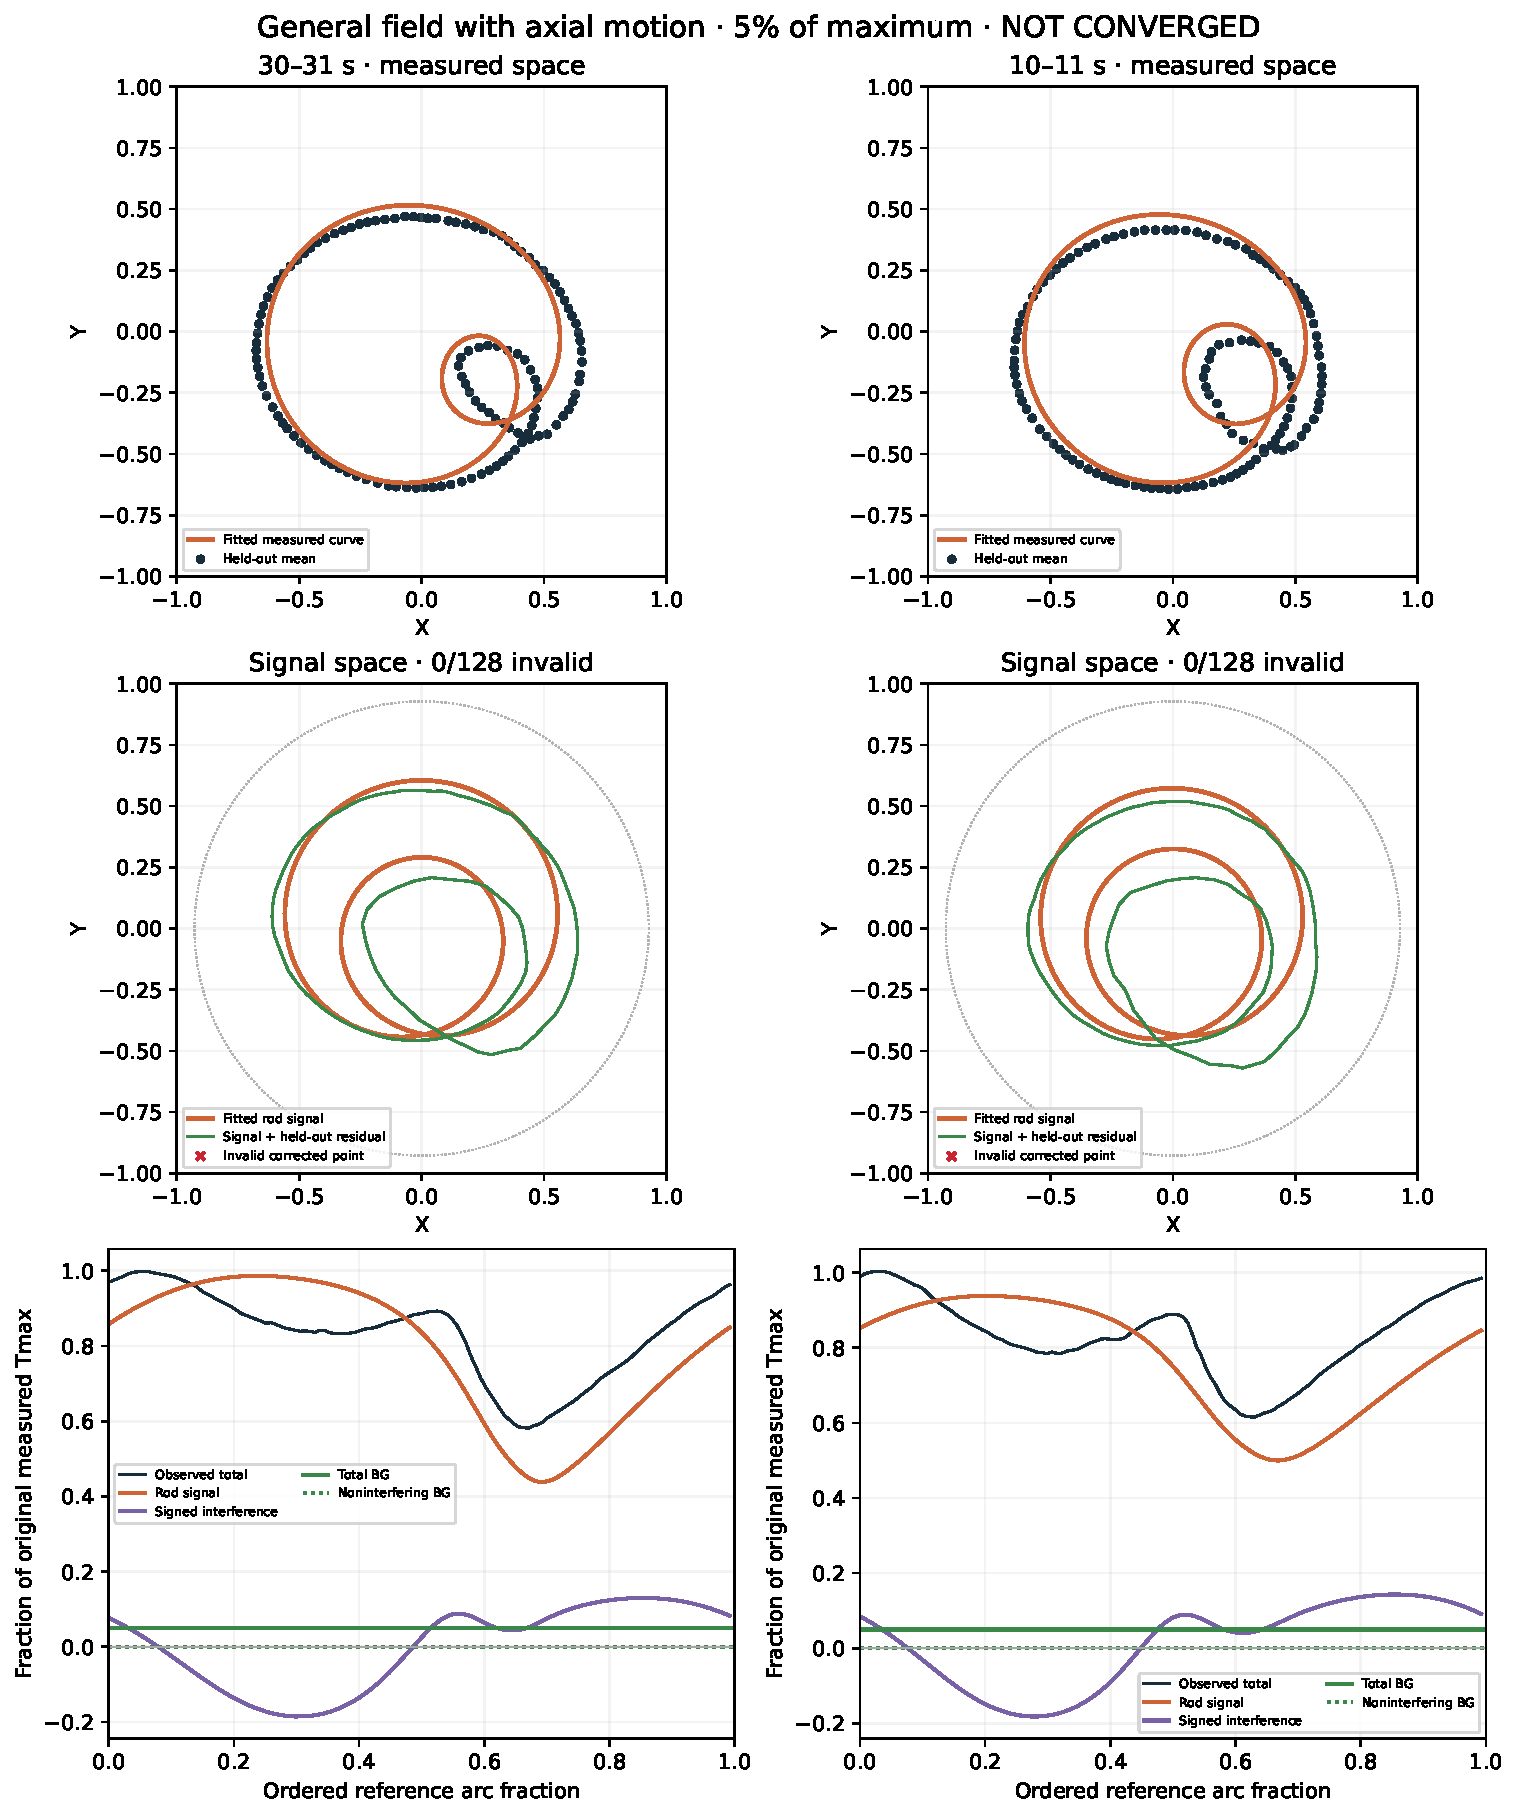
\includegraphics[width=\linewidth,height=.9\textheight,keepaspectratio]{figures/axial_5pct.pdf}
\newpage
\subsection{10\% of maximum}\label{case:axial:10pct}
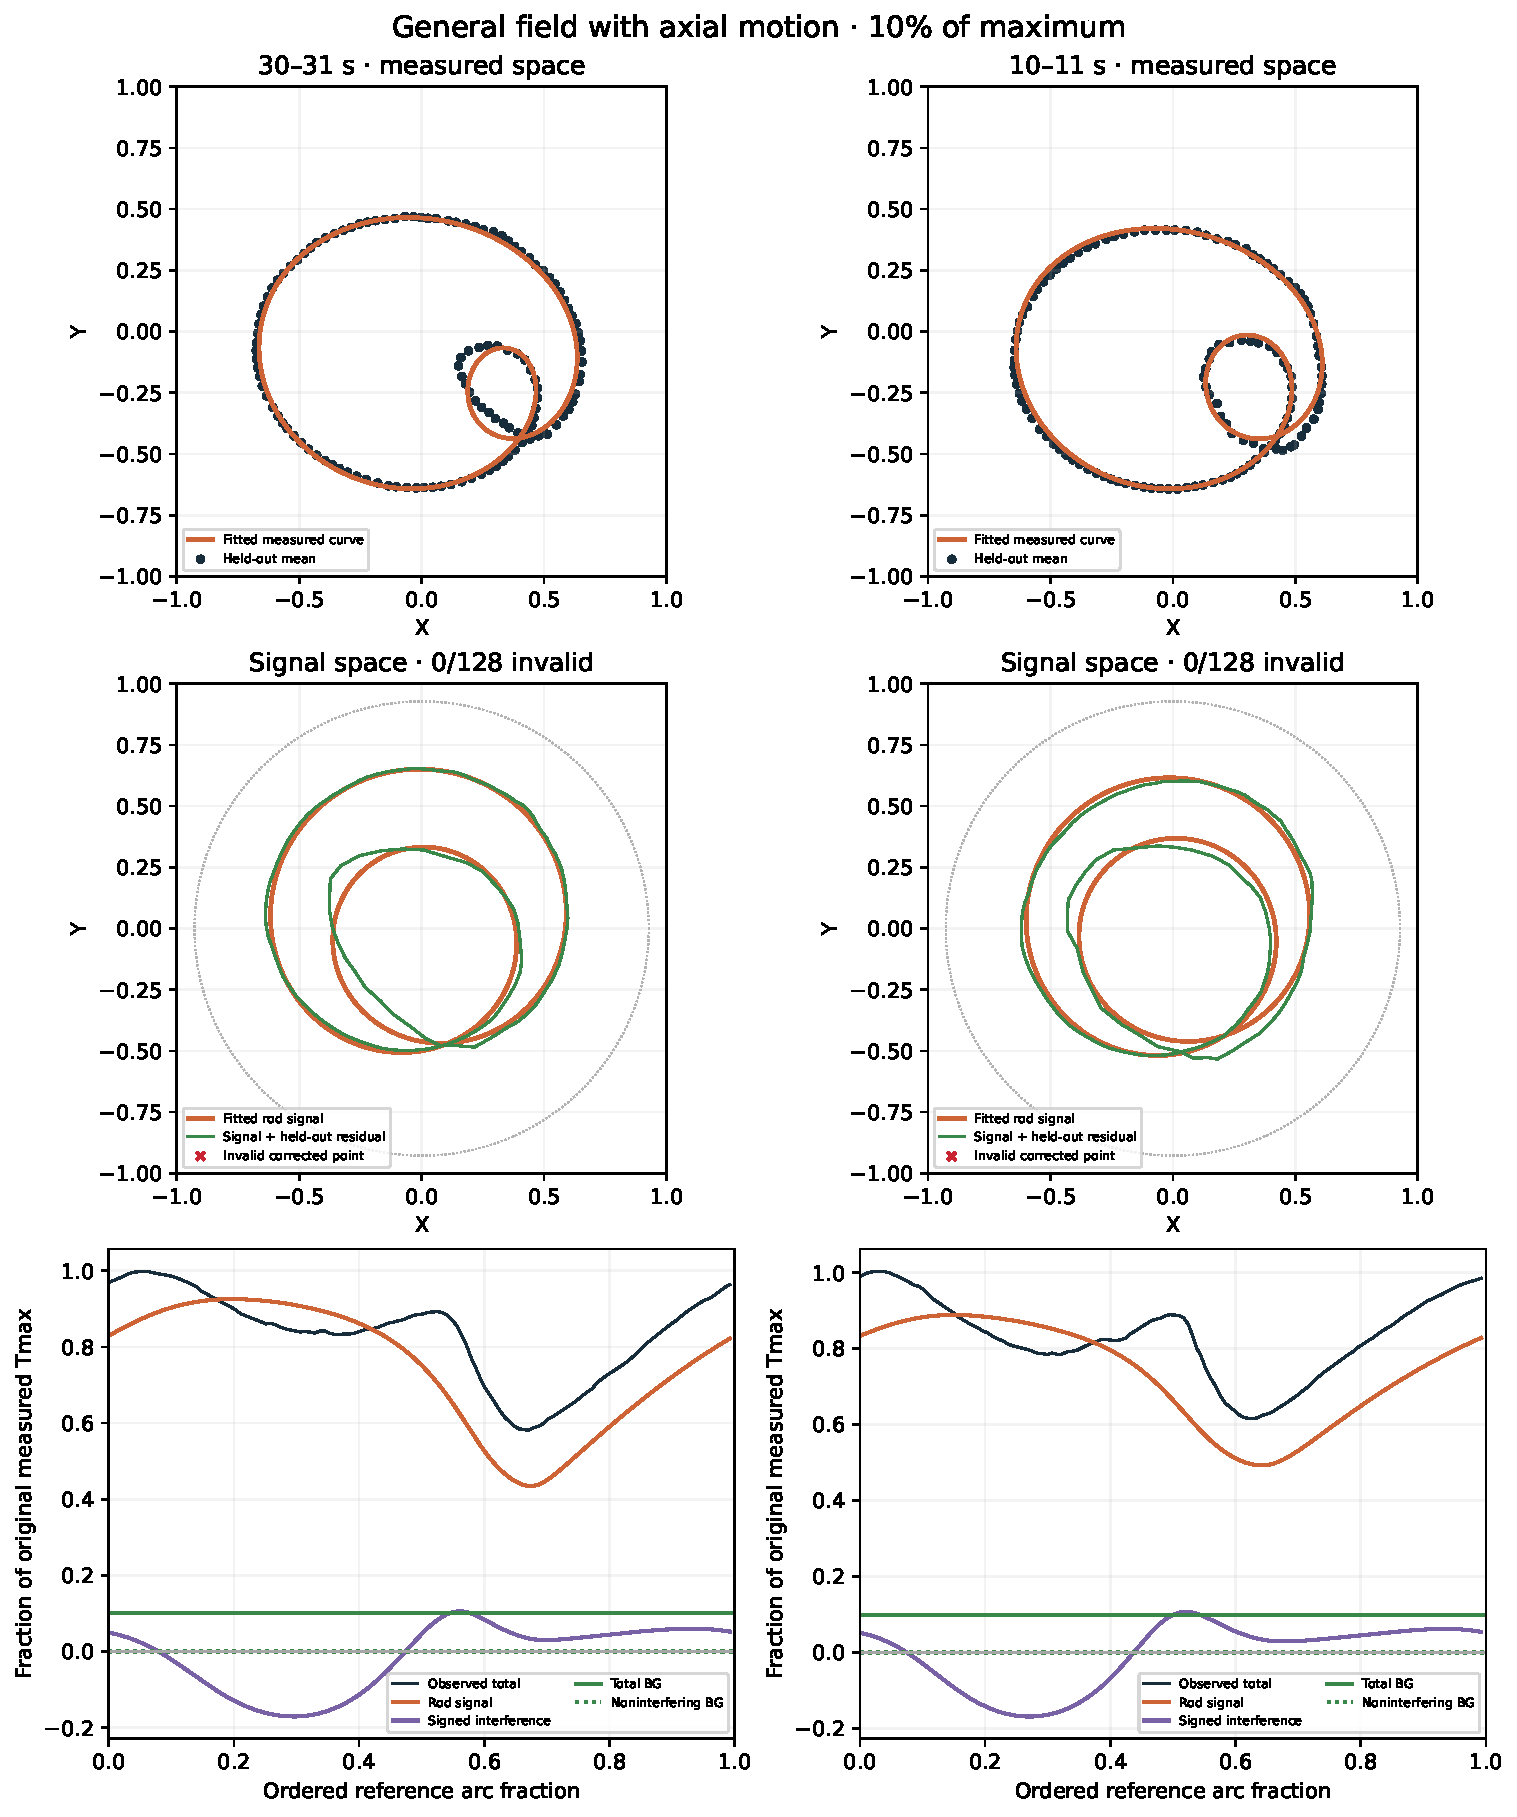
\includegraphics[width=\linewidth,height=.9\textheight,keepaspectratio]{figures/axial_10pct.pdf}
\newpage
\subsection{20\% of maximum}\label{case:axial:20pct}
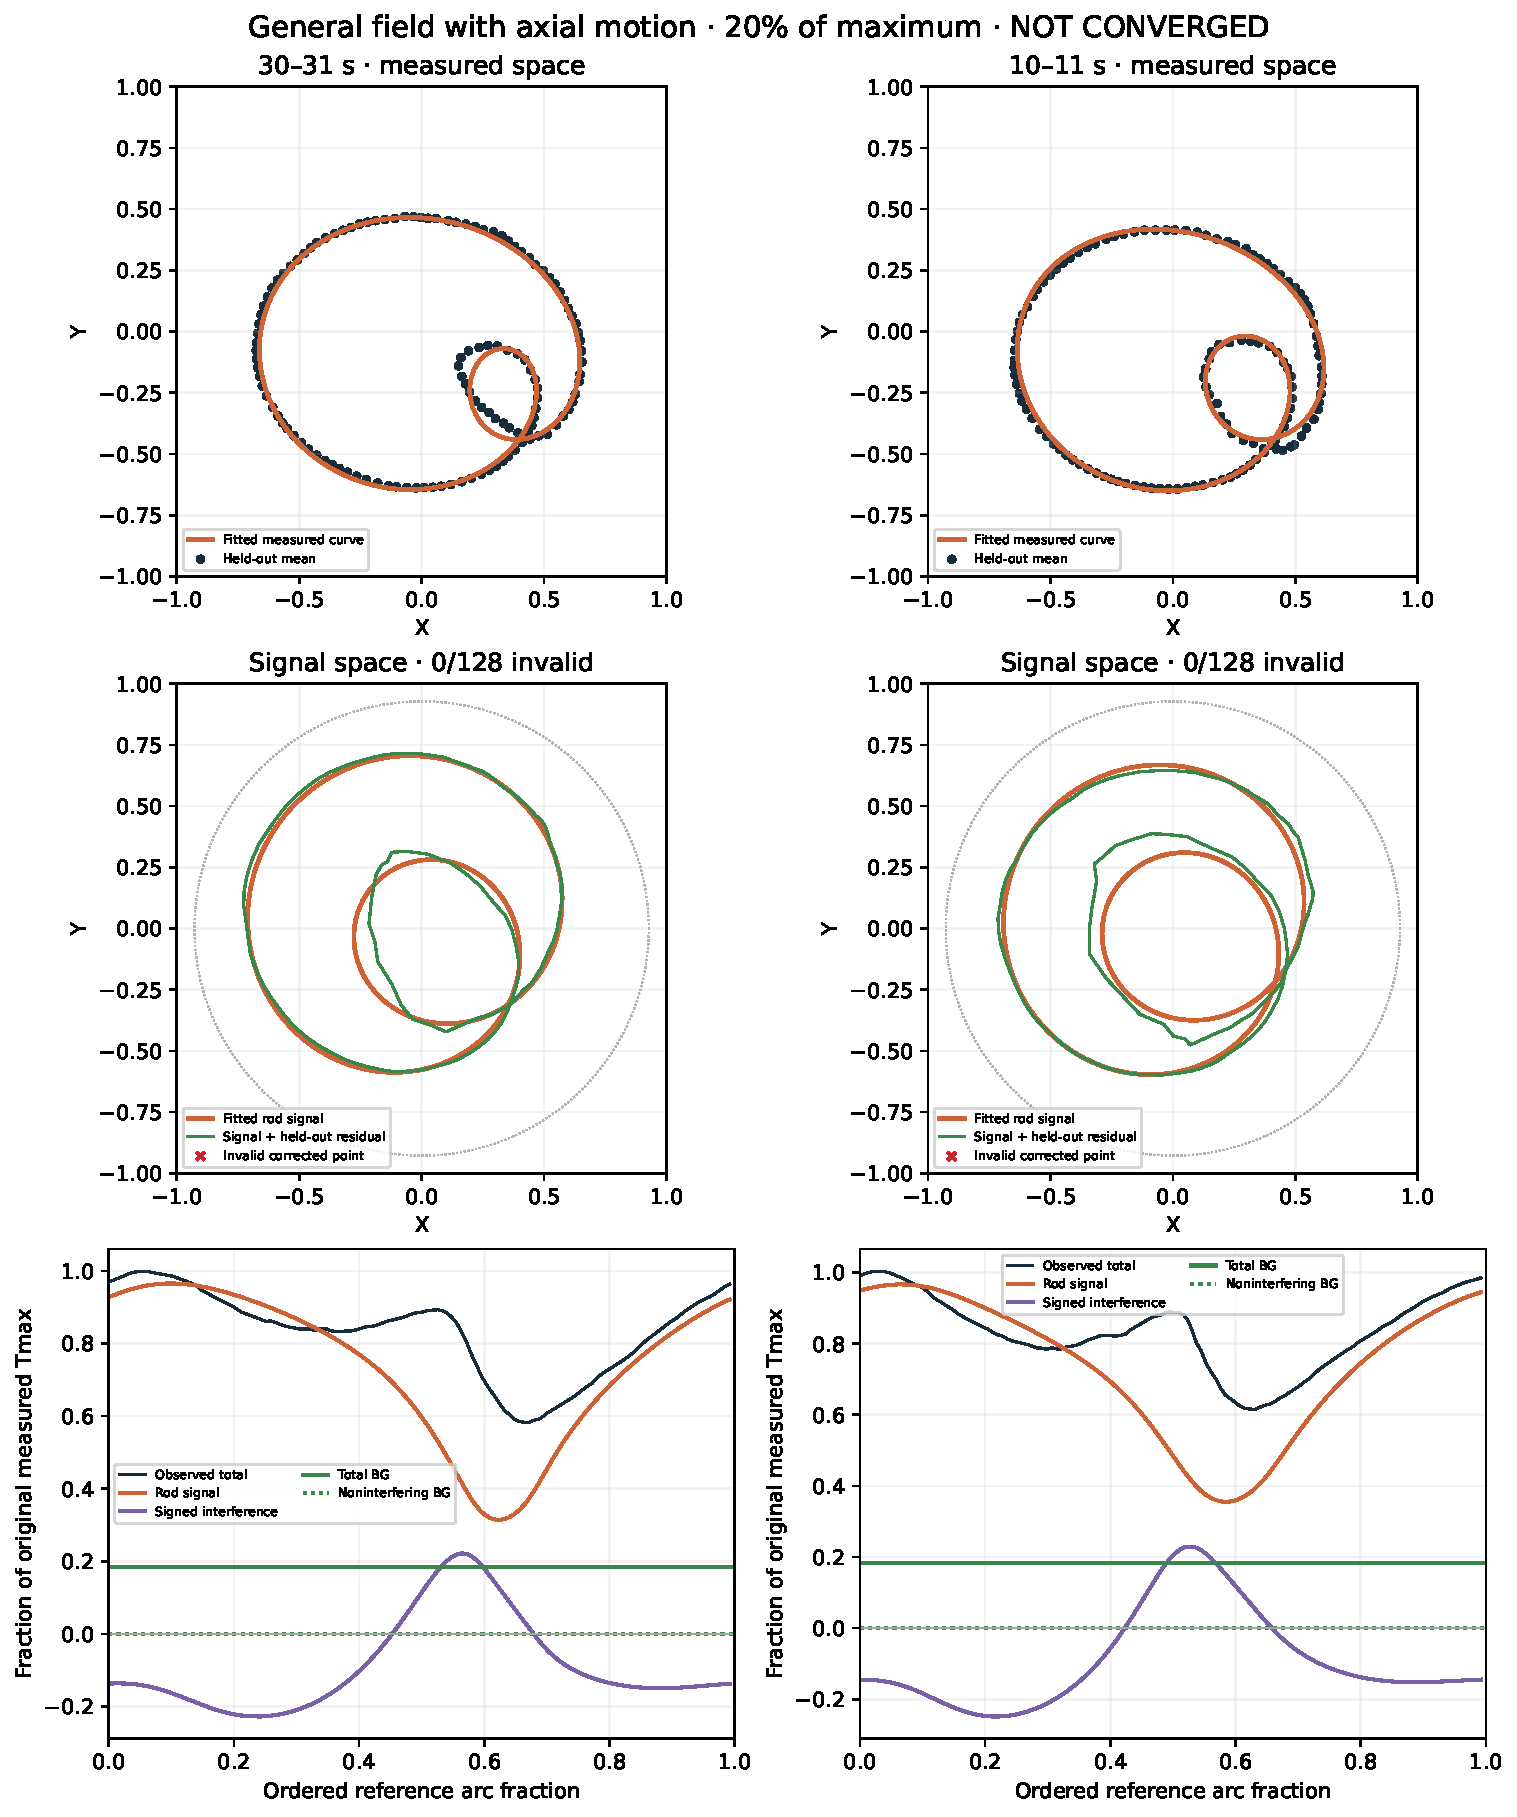
\includegraphics[width=\linewidth,height=.9\textheight,keepaspectratio]{figures/axial_20pct.pdf}
\newpage
\subsection{30\% of maximum}\label{case:axial:30pct}
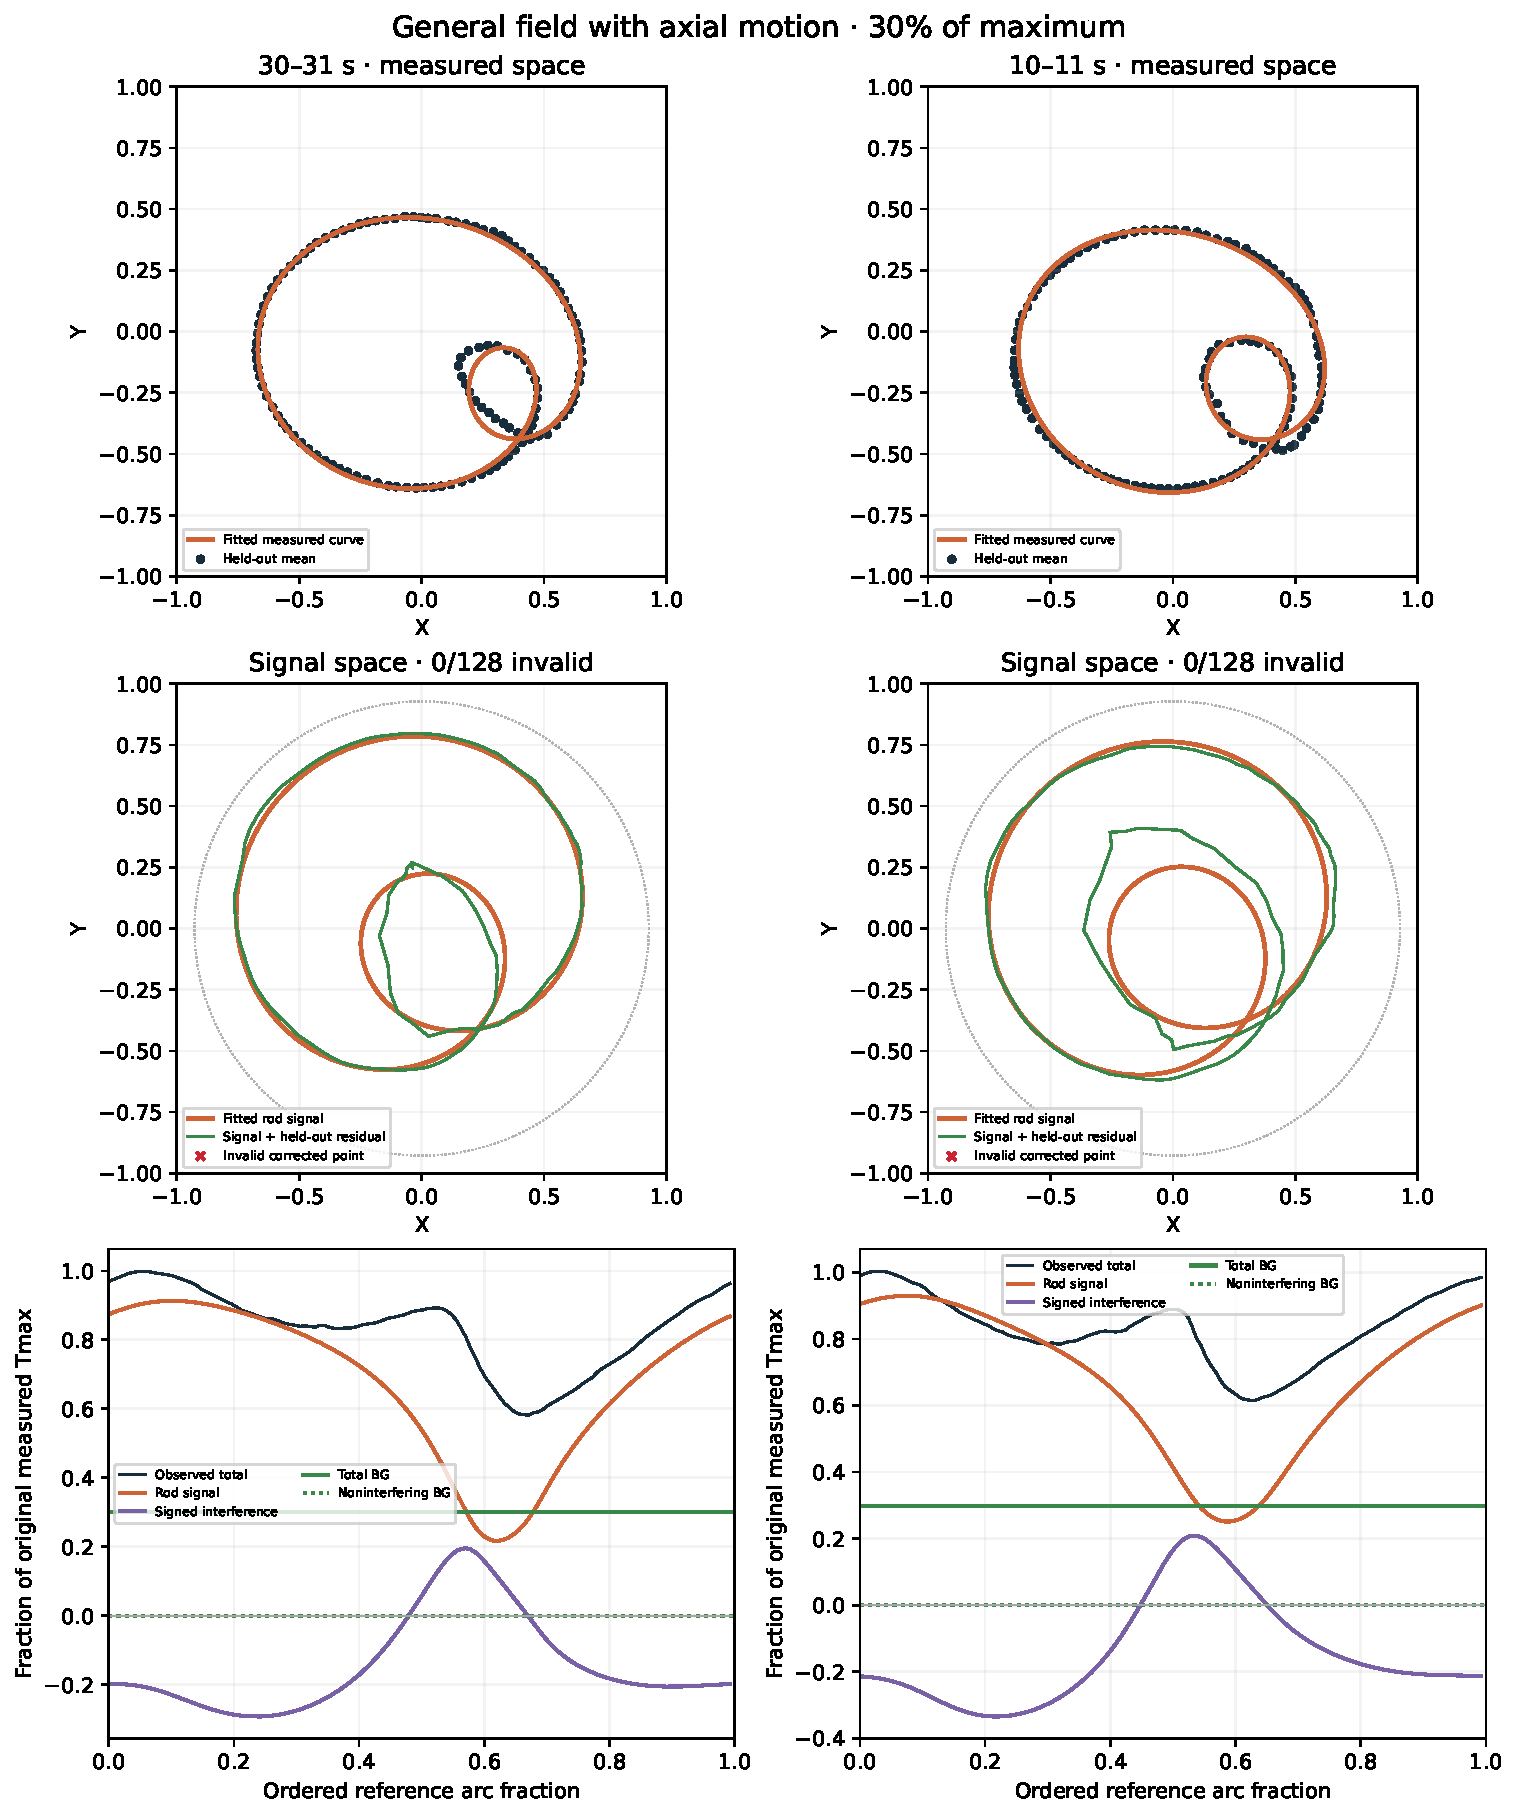
\includegraphics[width=\linewidth,height=.9\textheight,keepaspectratio]{figures/axial_30pct.pdf}
\newpage
\subsection{40\% of maximum}\label{case:axial:40pct}
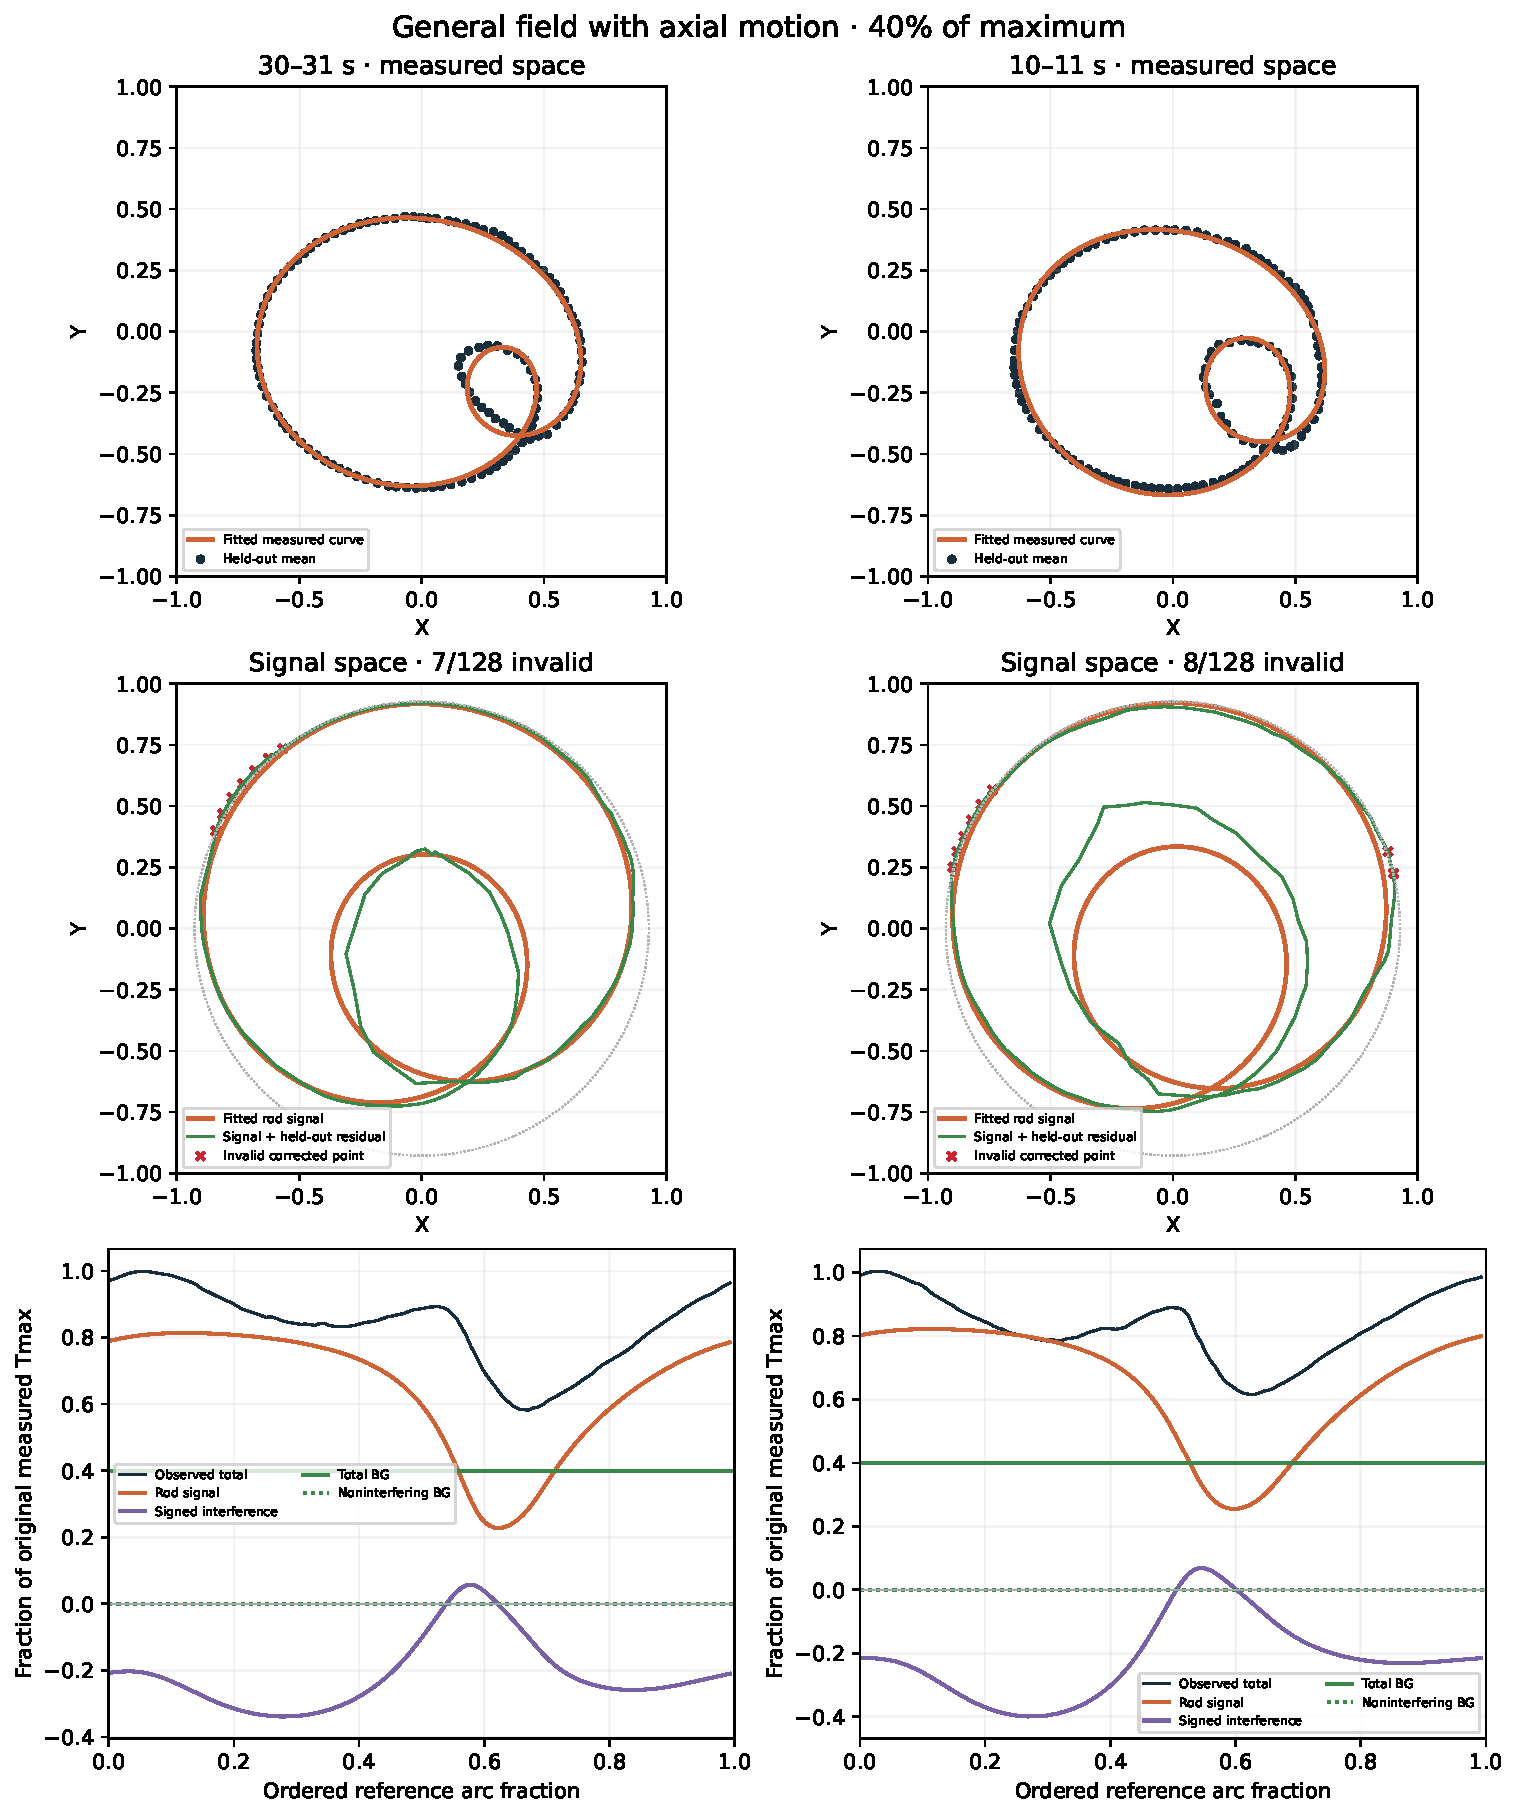
\includegraphics[width=\linewidth,height=.9\textheight,keepaspectratio]{figures/axial_40pct.pdf}
\newpage
\subsection{Representative sphere diagnostic: 10\% of maximum}
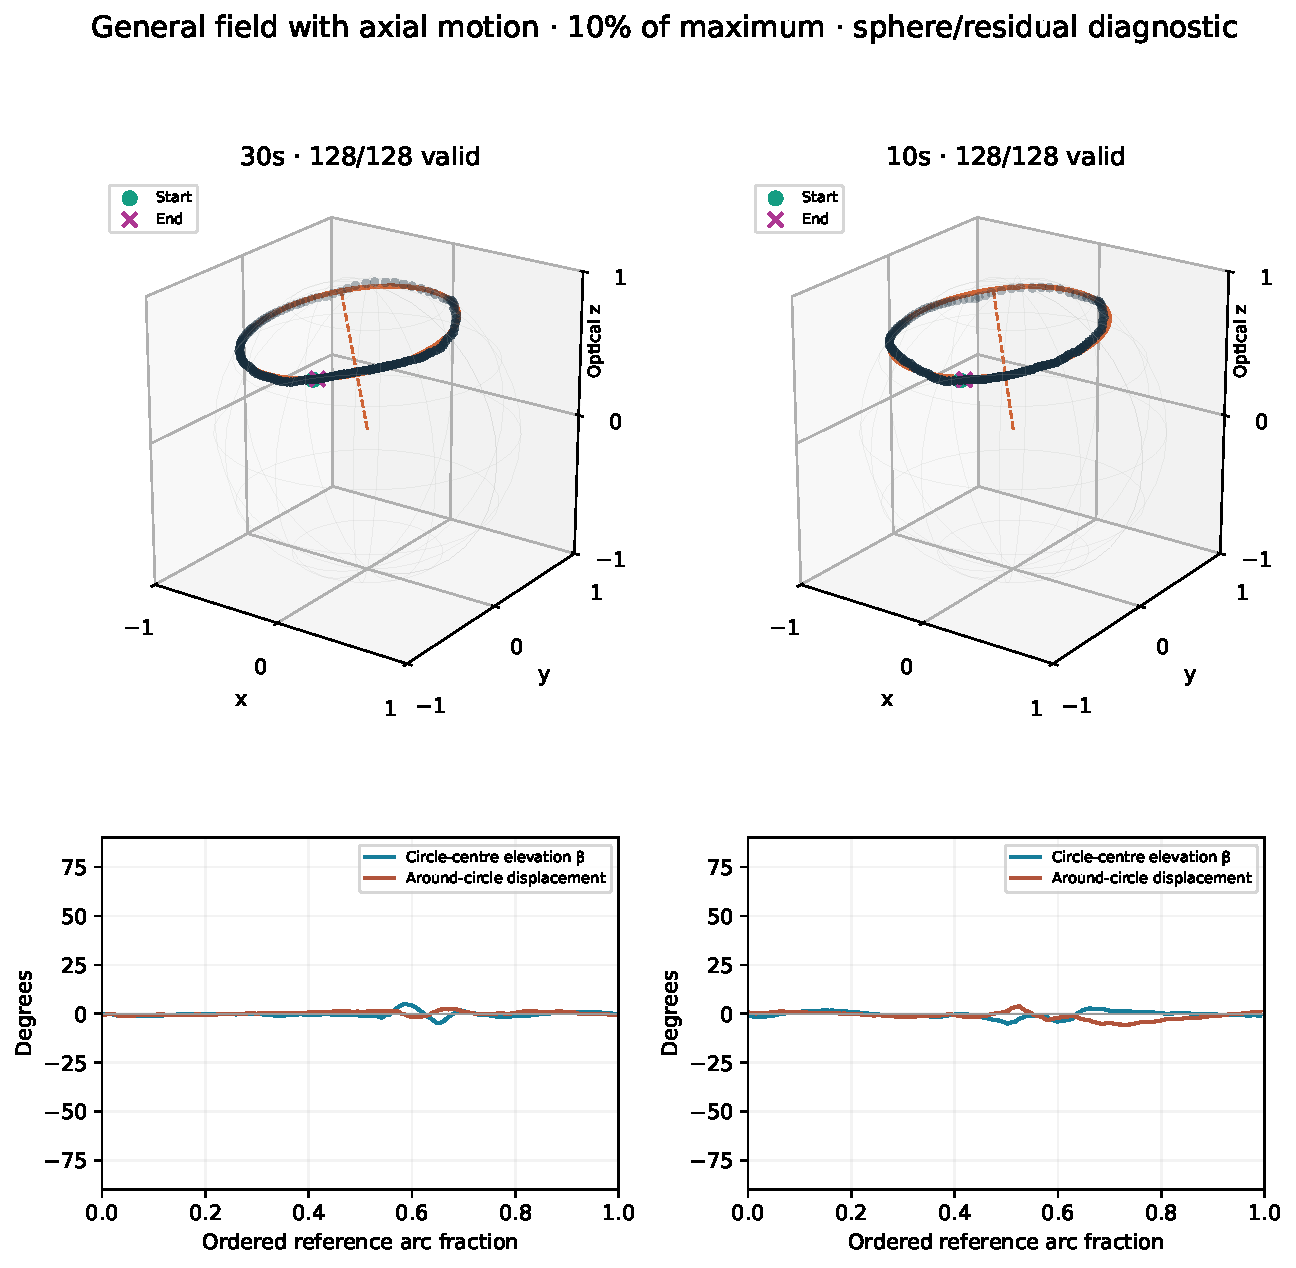
\includegraphics[width=\linewidth,height=.82\textheight,keepaspectratio]{figures/axial_sphere.pdf}
30s: 128/128 valid; matched geodesic RMS 1.67$^\circ$; oriented closure mismatch 0.00$^\circ$.\par
10s: 128/128 valid; matched geodesic RMS 2.79$^\circ$; oriented closure mismatch 0.00$^\circ$.\par
\newpage
\subsection{Local cone-referenced angular residual: 10\% of maximum}\label{local:axial}
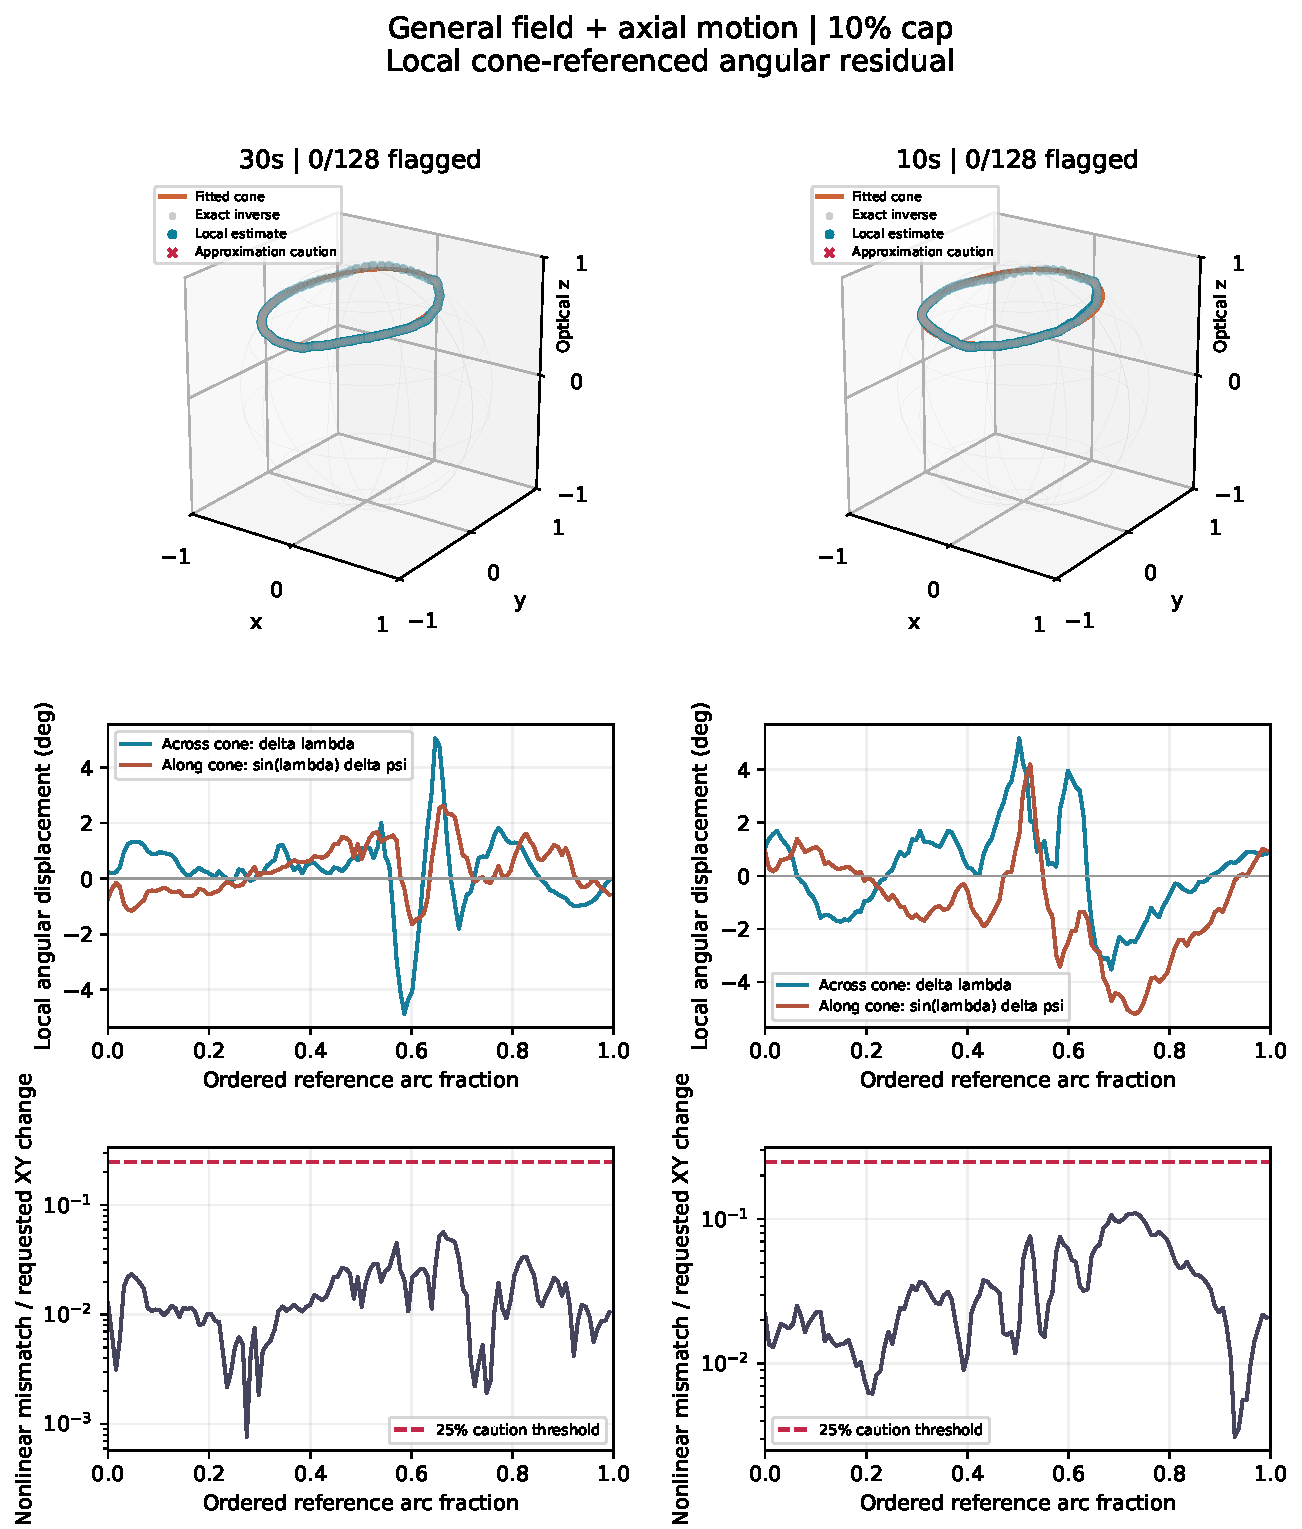
\includegraphics[width=\linewidth,height=.86\textheight,keepaspectratio]{local_residual/axial.pdf}
30s: local angular RMS 1.66$^\circ$; 0/128 caution flags; median nonlinear mismatch ratio 0.012.\par
10s: local angular RMS 2.79$^\circ$; 0/128 caution flags; median nonlinear mismatch ratio 0.026.\par
\newpage\section{Earlier tests retained as context}
\textbf{Stokes-restricted additive background.} Earlier fits restricted $(f_x,f_y)$ to a disk, while the current notebook-style additive model permits independent contrasts in a square. Earlier optima were inside the disk and changed little on relaxation. The user requested the simpler square form for current comparisons; the disk version is not duplicated as a separate sweep.

\textbf{Measured aperture mask.} Previous calculations compared the measured mirror mask against the annulus; selected held-out XY RMS changed by less than about0.0002 in that earlier setup. This does not justify importing old fit coefficients into the current reference pipeline. Current sweep uses the user-selected NA0.38 annulus throughout.

\textbf{Hole-edge variants.} Earlier widths0.03/0.10/0.25NA were tested with pure coherent edge backgrounds. The current representative uses0.10NA with additional noninterfering Stokes power. A poor edge-surrogate fit does not exclude arbitrary multiple reflections or edge scattering.

\textbf{Arbitrary overlap construction.} Allowing overlap to vary freely at each point can match trajectories without identifying a stationary field. It is a feasibility witness, not a fitted physical source model, and is not ranked as a competing cap sweep.

\textbf{Inverse sphere-circle fitting.} Earlier circle-only inverse fits exhibited collapse/cancellation degeneracy: an increasingly large correction could map observations into an increasingly tiny circle. Those tests remain evidence that circle closeness alone is insufficient, not a validated angle-recovery method.

\textbf{Flexible phase correspondence.} Previous sixteen-parameter monotone phase fits are not mixed with the fixed ordered-arc models here. Some old disagreement came from nonuniform final reference coordinates; those comparisons were explicitly withdrawn and repaired. The present plots use the repaired final-reference construction.

\textbf{Axial motion and finite-aperture focus.} Earlier50/150/300nm bounds and a finite-detector defocus sensitivity were conditional simulations, not measurements of hook geometry. The current axial family, when present, uses the300nm orbital bound with full pupil-phase overlap and the stated simple excitation focus factor. The separate finite-detector calculation is not silently included.

\section{Limits and next discussion}
No current fit proves a unique background composition or correct absolute angles. Low BG caps can stabilize subtraction while leaving measured or signal-space mismatch. More modes can reduce residuals but also permit cancellation. Pair balance alone does not distinguish gain error from every downstream-background mechanism. Current gain adjustment is fixed and shared, but not independently calibrated.

Uncapped searches have no BG-power upper bound, but geometry, log brightness and axial motion retain stated numerical/physical bounds. Multiple local starts are not a global search. Failure at a cap can depend on which local solution minimizes the training objective. Adaptive use of held-out clipping to choose further caps makes the overall sweep exploratory.

All scripts, per-fit parameters, train/test diagnostics, channel decompositions and figure sources are retained locally under model\_comparison/consolidated/. Files: simple.json, fields.json, axial.json, composition.json, metrics.csv, sphere\_summary.json, run.py and report.py. This report and its reproducible scripts and saved results are included in the project wrap-up commit. No new fits were performed for this notation revision.
\end{document}
